%%%%%%%%%%%%%%%%%%%%%%%%%%%%%%%%%%%%%%%%%%%%%%%%%%%%%%%%%%%%%%%%%%%%%
%% Submission template for the Journal of Computational Physics
%% (Elsevier). Built on the els-cas-templates "cas-sc" single-column
%% class used by Elsevier's CAS workflow.
%%%%%%%%%%%%%%%%%%%%%%%%%%%%%%%%%%%%%%%%%%%%%%%%%%%%%%%%%%%%%%%%%%%%%
\documentclass[a4paper,fleqn]{cas-sc}

% Use this option instead if the frontmatter overflows one page:
%\documentclass[a4paper,fleqn,longmktitle]{cas-sc}

%%%%%%%%%%%%%%%%%%%%%%%%%%%%%%%%%%%%%%%%%%%%%%%%%%%%%%%%%%%%%%%%%%%%%
%% Bibliography handling -- JCP uses numbered references.
%%%%%%%%%%%%%%%%%%%%%%%%%%%%%%%%%%%%%%%%%%%%%%%%%%%%%%%%%%%%%%%%%%%%%
\usepackage[numbers,sort&compress]{natbib}

%%%%%%%%%%%%%%%%%%%%%%%%%%%%%%%%%%%%%%%%%%%%%%%%%%%%%%%%%%%%%%%%%%%%%
%% Math, algorithms, and project-specific packages
%%%%%%%%%%%%%%%%%%%%%%%%%%%%%%%%%%%%%%%%%%%%%%%%%%%%%%%%%%%%%%%%%%%%%
\usepackage{../lyu}
\usepackage{algorithm}
\usepackage{algpseudocode}%[noend]
\usepackage{amsthm}
% \mathchardef\mhyphen="2D
\newcommand{\mhyphen}{\text{-}}

\newtheorem{theorem}{Theorem}
\newtheorem{lemma}[theorem]{Lemma}
\theoremstyle{definition}
\newtheorem{definition}[theorem]{Definition}
\theoremstyle{remark}
\newtheorem{remark}[theorem]{Remark}
\newtheorem{proposition}{Proposition}
\newtheorem{assumption}{Assumption}
\newtheorem{corollary}{Corollary}
\graphicspath{{../}}
\begin{document}
\let\WriteBookmarks\relax
\def\floatpagepagefraction{1}
\def\textpagefraction{.001}

\shorttitle{Stochastic branching particle method}
\shortauthors{L.~Lyu and H.~Lei}

\title[mode=title]{A stochastic branching particle method for solving non-conservative reaction--diffusion equations}

\author[1,2]{Liyao Lyu}
\ead{lyuliyao@math.ucla.edu}

\author[2,3]{Huan Lei}
\ead{leihuan@msu.edu}

\affiliation[1]{organization={Department of Mathematics, University of California, Los Angeles},
            addressline={520 Portola Plaza},
            city={Los Angeles},
            state={CA},
            country={USA}}

\affiliation[2]{organization={Department of Computational Mathematics, Science \& Engineering, Michigan State University},
            addressline={428 S Shaw Ln},
            city={East Lansing},
            state={MI},
            country={USA}}

\affiliation[3]{organization={Department of Statistics \& Probability, Michigan State University},
            addressline={619 Red Cedar Road},
            city={East Lansing},
            state={MI},
            country={USA}}

\begin{abstract}
We propose a stochastic branching particle-based method for solving nonlinear non-conservative advection–diffusion–reaction equations. 
The method splits the evolution into an advection–diffusion step, based on a linearized Kolmogorov forward equation and approximated by stochastic particle transport, and a reaction step implemented through a branching birth–death process that provides a consistent temporal discretization of the underlying reaction dynamics. This construction yields a mesh-free, nonnegativity-preserving scheme that naturally accommodates non-conservative systems and remains robust in the presence of singularities or blow-up. 
We validate the method on two representative two-dimensional systems: the Allen–Cahn equation and the Keller–Segel chemotaxis model. In both cases, the present method accurately captures nonlinear behaviors such as phase separation and aggregation, and achieves reliable performance without the need for adaptive mesh refinement.

\end{abstract}

\begin{keywords}
particle methods \sep
stochastic branching \sep
reaction-diffusion \sep
chemotaxis \sep
aggregation
\end{keywords}

\maketitle

\section{Introduction}
The advection--diffusion--reaction (ADR) type partial differential equations (PDEs) have attracted much interest in physics, biology, and engineering for modeling various phenomena relevant to chemical reactions, transport, and collective behaviors in biological systems \cite{hundsdorfer2013numerical}. Traditional grid-based methods, such as finite difference~\cite{hoff1978stability}, finite element~\cite{codina1998comparison}, and discontinuous Galerkin schemes~\cite{ayuso2009discontinuous,xia2009application}, have achieved great success in solving many of these problems. However, from a numerical perspective, an essential challenge in solving such PDEs lies in handling nonlinearities and singular structures in certain cases, e.g., the aggregation phenomena of the Keller--Segel (KS) model \cite{keller1970initiation} and the interfacial dynamics of the Allen--Cahn (AC) model \cite{Allen_Cahn_1979}.  
Mesh-based discretizations approximate solutions in function spaces that may not be well-suited for capturing the blow-up or highly localized behavior, often resulting in reduced accuracy or numerical instabilities, and requiring additional numerical treatments.


Particle-based approaches offer a natural alternative by representing the solutions as empirical measures, which are particularly effective for problems exhibiting concentration or blow-up phenomena. 
Existing particle methods, such as the particle-in-cell method~\cite{birdsall2018plasma, hockney2021computer} for solving the Vlasov--Poisson equation, are often based on well-established  underlying physical laws. In this setting, particle dynamics can be derived from the explicit micro-scale governing equations. In contrast, the explicit physical laws are often unknown for general non-conservative ADR type PDEs, where effective interactions may be highly nonlinear, system-specific, or even not well characterized. For example, in many biological and chemical systems such as chemotaxis, the micro-scale interactions remain poorly understood, which limits the applicability of traditional particle-based approaches.
To extend particle-based methods beyond physically motivated settings, blob methods~\cite{craig2016blob,carrillo2019blob,huang2017error} and semi-Lagrangian particle schemes~\cite{qiu2010conservative,qiu2011conservative,qiu2011positivity} have been developed for conservative PDEs.
These approaches are based on the mean-field perspective, in which the empirical measures of interacting particle systems converge to the solution of the original PDE. This mathematical framework establishes a rigorous link between the particle dynamics and the continuum equations and does not rely on explicit microscale physical laws. Despite these advances, there is still no unified particle-based framework for systematically discretizing nonlinear and non-conservative PDEs, especially in the presence of singularities, sharp interface or blow-up phenomena.

Machine learning-based numerical PDE algorithms, such as Deep Galerkin Methods~\cite{sirignano2018dgm}, Deep Ritz method~\cite{yu2018deep}, and Mixed Residual method~\cite{lyu2022mim}, have attracted significant attention in recent years. By leveraging the strong representability of neural networks, these methods are particularly promising for solving high-dimensional problems. In the context of particle-based approaches, coupling neural networks with the Feynman-Kac formula~\cite{han2024deep, hutzenthaler2021speed, nguwi2024deep,beck2021deep} or backward stochastic differential equations (SDEs) ~\cite{han2017deep, han2018solving, hure2020deep} has also emerged as a powerful strategy for solving a broad class of PDEs. Nevertheless, the approximation capability of neural networks is fundamentally grounded in the universal approximation theorem that targets continuous solutions on compact sets.
As a result, neural-network–based solvers may face intrinsic difficulties when dealing with nonlinear, non-conservative PDEs that develop singularities or blow-up phenomena, where discontinuities or concentration effects play a central role.

In this work, we propose a \textit{stochastic branching particle method} to address these challenges. 
At each time step, the original PDE is locally linearized and approximated by the Kolmogorov forward equation, which establishes a direct connection between the PDE and the stochastic particle dynamics.  Unlike approaches that rely on explicit physical laws or mean-field limit arguments, this framework establishes a systematic particle-based discretization applicable to general nonlinear and non-conservative PDEs. 
%
A key feature of the method is a particle-level birth–death mechanism, introduced to represent non-conservative reaction terms by allowing the number of particles to evolve consistently with the underlying reaction dynamics. The only step that invokes a continuity assumption is the interpolation of the empirical measure, which can be replaced by blob- or kernel-based representations. Consequently, the developed method does not fundamentally rely on continuity and is well-suited for problems with singularities or blow-up phenomena. 
%
From a numerical perspective, the proposed method is broadly compatible with existing stochastic interpretations of reaction–diffusion systems. For example, in the case of chemotaxis, it aligns with the mean-field derivation of the KS equation from moderately interacting particles developed by Stevens~\cite{Stevens_SIAM_2000}. However, our formulation is not restricted to this setting and applies generally to nonlinear ADR systems with non-conservative terms.

% From a stochastic particle perspective, the algorithm is naturally consistent with the physical intuition behind Keller–Segel dynamics, in line with Stevens' mean-field derivation of the Keller–Segel equations from moderately interacting particle systems \cite{Stevens_SIAM_2000} and can be applied naturally to a broader class of advection–diffusion–reaction systems.
% formulation is closely related to Stevens’ mean-field derivation of Keller--Segel equations from moderately interacting particle systems \cite{Stevens_SIAM_2000}. Unlike  \cite{Stevens_SIAM_2000}, we develop a finite-$N$ particle discretization based on local Kolmogorov linearization and a particle-level birth-death update, which directly handles the nonlinear and nonconservative terms and extends to a class of advection–diffusion–reaction systems.  


To illustrate the effectiveness of the proposed method, we consider two representative non-conservative reaction–diffusion systems: the AC equation for the phase separation with interfacial motion and nonlinear reactions,  
and the KS chemotaxis model for the aggregation-driven blow-up dynamics~\cite{keller1970initiation, patlak1953random}. 
While the AC equation serves to demonstrate the generality of our method, the KS model provides a more challenging test problem and is the primary focus of the present study. In particular, we consider the two-dimensional KS chemotaxis model as the theme problem, which takes the form 
\begin{equation}\label{equ:KS}
\begin{aligned}
\partial_t u - \nabla \cdot ( \nabla u - \chi(u) \nabla v) &= f_u(u,v), & \bx\in \mathbb{T}^2 , t\in(0,T), \\
\partial_t v - \Delta v &= f_v(u,v), & \bx\in \mathbb{T}^2 , t\in(0,T),
\end{aligned}
\end{equation}
where $u$ and $v$ represent the cell density and chemical concentration, respectively. $\chi$ represents the chemotactic sensitivity, and $f_u$ and $f_v$ represent the production or decay rate.  For simplicity, we focus on periodic boundary conditions or unbounded domains, though the framework can be extended to more general boundary settings in future research.  
%The KS system~\eqref{equ:KS} has been extensively studied over the past several decades, with numerous works addressing both analytical properties and numerical methods across model variants and dimensions. 
In two dimensions, it is well understood that both parabolic–elliptic and fully parabolic cases can exhibit finite-time blow-up to a Dirac-delta profile when the initial mass is sufficiently large~\cite{herrero1997blow, perthame2007transport}. Furthermore, in the three-dimensional parabolic–elliptic case, an alternative self-similar blow-up profile of the form $ C(T-t+\vert \mb x\vert ^2)^{-1}$ has also been identified in the literature~\cite{giga2011asymptotic,souplet2019blow}. 

On the numerical side, many notable methods have been developed for the KS systems. The finite-volume method~\cite{filbet2006finite,chertock2008second,chertock2018high} achieves efficient and positivity-preserving simulations for chemotaxis and haptotaxis models.  
%
Shen et al.~\cite{shen2020unconditionally} introduced an energy-dissipative and bound-preserving formulation, subsequently extended by Chen et al.~\cite{chen2022error} to a fully discrete finite element scheme for the 2D parabolic–elliptic KS, which reproduces finite-time blow-up under assumptions analogous to the continuous setting. 
Liu and Wang~\cite{liu2018positivity} reformulated the equations via the Le Ch\^atelier principle to construct positivity-preserving schemes. Discontinuous Galerkin methods have also been applied to KS systems~\cite{zhong2024direct, li2017local,epshteyn2009new}, in addition to various mesh-based finite element, finite volume, and domain-decomposition techniques for 3D fully parabolic models~\cite{epshteyn2019efficient, strehl2013positivity}. For particle-based approaches, the most relevant work is the recently proposed stochastic interacting particle–field algorithm~\cite{wang2025novel,hu2024stochastic,chertock2025hybrid}. However, this approach does not deal with the non-conservative equations at the particle level, limiting its applicability to the broader class of nonlinear non-conservative PDEs. 

We address this challenge by explicitly coupling a SDE-based advection--diffusion process with a particle-level birth--death mechanism for reactions, which overcomes the limitations of traditional methods and yields a particle measure discretization that remains robust near concentration and blow-up. We validate the method on two-dimensional KS benchmarks, including near blow-up and nonlinear growth, and compare with the standard grid-based method, observing the expected $1/\sqrt{N}$ scaling with the particle number.
%
The remainder of the paper is organized as follows: Section 2  and 3 present the stochastic branching method for a non-conservative ADR equation and the convergence analysis; Section 4 extends the approach for the KS systems; Section 5 reports numerical results and Section 6 discusses extensions and outlook.

% This work makes three contributions. (\Rmnum{1}) We introduce a stochastic branching framework that couples SDE-based advection–diffusion with a birth–death mechanism for reactions, yielding a particle–measure discretization that is not tied to smooth function spaces and remains effective near concentration and blow-up. (\Rmnum{1}) We derive the scheme via local Kolmogorov linearization and an operator splitting, giving a transparent PDE–SDE correspondence and an implementable algorithm with Fourier/kernel reconstructions of empirical measures. (\Rmnum{1}) We validate the method on two-dimensional KS benchmarks—including near-blow-up and nonlinear growth—against standard grid-based baselines, observing the expected $1/\sqrt{N}$ scaling with particle number. We also discuss extensions to other reaction–diffusion systems (Gray–Scott, Allen–Cahn, Schnakenberg) and paths toward higher-dimensional settings, with details deferred to the Discussion


% In summary, we propose a novel stochastic branching method for solving the Keller–Segel chemotaxis model, which overcomes the limitations of traditional numerical methods by efficiently handling singularities and nonlinearities at particle level. A heuristic derivation of the algorithm is presented in the current version and will be discussed in detail in future work. Although our focus here is on the two-dimensional Keller–Segel model, the proposed framework is general and can be applied to a broad class of reaction–diffusion systems, such as the Gray–Scott model, the Allen–Cahn equation, and Schnakenberg pattern formation. Furthermore, by leveraging recent advances in density estimation techniques~\cite{novikov2021tensor, tang2025wavelet, sheng2025approximation, tang2024solving}, our approach can be naturally extended to higher-dimensional systems. The effectiveness of the method is demonstrated through several numerical examples, highlighting both its robustness and potential for generalization.

\section{Stochastic branching method}
Let us start with the following scalar non-conservative advection-diffusion–reaction system on the $d$-dimensional torus $\mathbb{T}^d$ for a time $t \in (0, T]$:
\begin{subequations}\label{equ:reaction-diffusion}
\begin{align}
\partial_t u &= \nabla \!\cdot\! \big( a(u) u \big) + D \Delta u + r(u) u, & \text{for } (x, t) \in \mathbb{T}^d \times (0, T], \label{equ:pde} \\
u(x, 0) &= u_0(x), & \text{for } x \in \mathbb{T}^d. \label{equ:ic}
\end{align}
\end{subequations}
Here, $u(x,t)$ is the scalar field, $a(u): \mathbb{R}_{+} \to \mathbb{R}^d$ is the advective velocity, $D > 0$ is the diffusion coefficient, and $r(u): \mathbb{R}_{+} \to \mathbb{R}$ is the reaction rate.
Let $S(N,t)=\{\bX^i\}_{i\in\mathcal I^N_t}$ denote a set of particles at time $t$ whose initial population is $N$, where the particles' indices are numbered consecutively in the index set $\mathcal I^N_t$ and $\bX^i(t)$ denote the position of the $i\mhyphen$th particle. The associated empirical (finite) measure is
\begin{equation}
    t \to \mu^N(t,\intd \bx) =  \frac{1}{N}\sum_{i\in \mathcal I^N_t}\delta_{\bX^i(t)},
\end{equation}
where $\delta_\bx $ denotes the Dirac measure at $\bx\in \mathbb{T}^d$. The core idea of particle-based methods is to approximate the PDE solution by the limit of the empirical measure
\[
\mu(t,\mathrm{d}\bx) = \lim_{N\to\infty} \mu^N(t,\mathrm{d}\bx).
\]
Since Eq. \eqref{equ:reaction-diffusion} is non-conservative, the total mass of the system is not preserved. Consequently, both $\mu^N$ and its limit $\mu$ should be viewed as finite measures rather than probability measures.


\subsection{Initial condition and Normalization}
To connect the solution $u(t,\bx)$ to the measure $\mu(t,\mathrm{d}\bx)=\rho(t,\bx) \intd \bx$, we introduce a linear transformation between them. 
Without loss of generality, we assume that the initial measure $\mu(0,\cdot)$ is a probability measure with total mass $1$, and define
\begin{equation*}
    u(t,\bx)\,\mathrm{d}\bx = Z \,\mu(t,\mathrm{d}\bx), \quad 
Z = \int_{\Omega} u(0,\bx)\,\mathrm{d}\bx,
\end{equation*}
where $Z$ denotes the total initial mass.
Thus $\rho(0,\cdot)$ is a probability density
\[
\rho(0,\mathbf{x}) \;=\; \frac{u(0,\mathbf{x})}{Z},
\]
and we can sample the initial particle positions independently from $\rho(0,\cdot)$ (e.g., via Metropolis–Hastings) to form $S(N,0)=\{\mathbf{X}^i_0\}_{i=1}^N$. 
Substituting $u=Z\rho$ into~\eqref{equ:reaction-diffusion}  yields
\begin{equation}\label{equ:normalized_diffusion_reaction}
\partial_t \rho 
= \nabla \cdot \left( \tilde a(\rho)\rho \right)+ D \Delta\rho 
  + \tilde r(\rho)\rho,
\end{equation}
with rescaled coefficients
\[
\tilde a(\rho) = a(Z\rho),  
\qquad \tilde r(\rho) = r(Z\rho).
\]
Since reactions generally change the total mass, $\int_{\Omega}\rho(t,\mathbf{x})\,\mathrm{d}\mathbf{x}$ may not equal $1$ for $t>0$. Rather, it tracks the mass of $u$ via $\int_{\Omega} u(t,\mathbf{x})\,\mathrm{d}\mathbf{x} = Z \int_{\Omega} \rho(t,\mathbf{x})\,\mathrm{d}\mathbf{x}$.

\subsection{Operator Splitting}
To approximate the solution of the PDE, we discretize the time interval $[0,T]$ with step size $\tau>0$ and grid points
\[
0 = t_0 < t_1 < \cdots < t_M = T,\qquad \tau=t_{n+1}-t_n.
\]
Then an operator-splitting strategy is used to separate the dynamics according to their physical mechanisms. 
Equation~\eqref{equ:normalized_diffusion_reaction} can be written as
\begin{equation}\label{eq:rho-pde}
\partial_t \rho = \mathcal{A}(\rho) + \mathcal{B}(\rho) ,
\end{equation}
where the operators $\mathcal{A}$ and $\mathcal{B}$ correspond to
\begin{align}
\mathcal{A}(\rho) =& \nabla \cdot \left( \tilde a(\rho)\rho \right) + D\Delta\rho  ,\label{eq:operator-A} \\
\mathcal{B}(\rho) =& \tilde r(\rho)\rho \label{eq:operator-B}.
\end{align}
Here, $\mathcal{A}$ describes the advection--diffusion dynamics, while $\mathcal{B}$ accounts for the reaction mechanism (e.g., proliferation or death).  The evolution of the exact solution over $t$ can be expressed formally as
\begin{equation}\label{}
\rho(t,\bx) = \exp\left( t (\mathcal{A} + \mathcal{B}) \right)\rho(0,\bx).
\end{equation}
Since $\mathcal A$ and $\mathcal B$ are nonlinear, $\exp\!\big(t(\mathcal{A}+\mathcal{B})\big)$ is to be read as formal notation for the solution flow of \eqref{eq:rho-pde}. This flow cannot be evaluated explicitly, so we adopt a first-order Lie--Trotter operator splitting \cite{trotter1959product}. For \emph{linear} semigroups the splitting is justified, in the limit, by the Trotter product formula
\begin{equation}
\exp\!\left( t (\mathcal{A} + \mathcal{B}) \right) 
= \lim_{M\to\infty} \Big( \exp\!\left(\tfrac{t}{M} \mathcal{B}\right) 
                          \exp\!\left(\tfrac{t}{M} \mathcal{A}\right) \Big)^M .
\end{equation}
For the nonlinear operators $\mathcal A,\mathcal B$ considered here this identity no longer holds exactly; we use it only as a formal motivation for the first-order splitting, whose time-discretization error is quantified rigorously in Theorem~\ref{prop:time_discrete_particle}.
At the discrete level, we approximate $\rho(t_{n+1},\cdot)$ by
\begin{equation}
\rho_{n+1} = \exp(\tau \mathcal{B}) \exp(\tau \mathcal{A}) \rho_n ,
\end{equation}
for $n=0,\cdots,M-1$.
This scheme provides a simple and efficient first-order approximation; 
higher-order splittings, such as Strang splitting \cite{strang1968construction}, may be employed for improved accuracy.
In practice, this decomposition allows us to design particle-based updates for each subprocess separately:
\begin{equation}\label{eq:lie-trotter}
\rho_n^\ast = \exp(\tau \mathcal{A})\rho_n, 
\qquad 
\rho_{n+1} = \exp(\tau \mathcal{B})\rho_n^\ast.
\end{equation}

\subsection{Advection Diffusion Step}
\label{sec:adevection_diffusion}
In this step, we propagate particles under the advection–diffusion dynamics, where each particle follows a stochastic path determined by both a drift and a diffusion term. At time step $n$, let $S^N_n = \{\bX^i_n\}_{i\in \mathcal I^N_n}$ denote  a set of particles  whose initial population is $N$, which induce the empirical measure 
\[
\mu^N_n= \frac{1}{N}\sum_{i\in \mathcal I^N_n}\delta_{\bX^i_n}
\] 
approximates the solution at step $n$, i.e.,  $\mu^N_n (\intd \bx) \approx \mu_n(\intd \bx) = \rho_n(\bx)\intd \bx$. 
Our goal is to evolve these particles according to the transition probability $p(\bx,s;\by,t)$, which leads to an updated empirical measure
\[\mu^{N,*}_n = \int p(\bx,t_n;\by,t_n+\tau)  \mu^N_n(\intd \bx) =   \frac{1}{N}\sum_{i\in \mathcal I^N_n}\delta_{\bX^{i,*}_n}
\]  
reflecting the action of the advection--diffusion operator on the density.
By the Kolmogorov forward equation, the transition density $p(\bx,s;\by,t)$ satisfies 
\begin{equation}
    \partial_t p = \tilde {\mathcal A }p := - \nabla \cdot(b  p) + \frac{1}{2}\nabla^2:(\sigma \sigma^\top p) 
\end{equation}
with initial condition $\lim_{t\to s^+} p(\bx,s;\cdot,t) = \delta_\bx$. By matching the differential operator $\mathcal A$ with the target PDE \eqref{equ:reaction-diffusion}, we have 
\begin{equation}
    b(x) = -\tilde a(\rho^N_n(x)), \quad \tfrac{1}{2}\sigma \sigma^\top = D\,I_d
    \quad\text{(equivalently } \sigma=\sqrt{2D}\,I_d\text{)},
\end{equation}
where $\rho^N_n(x)$ represents the interpolated probability density of $\mu^N_n$ and will be discussed in Sec. \ref{sec:interpolation}.
%
Accordingly, the evolution of each particle $\bX^i_n$ as a stochastic process satisfying the It\^o stochastic differential equation
\begin{equation}\label{equ:overd_langevin}
    \intd \bX^i_n = b(\bX^i_n) \intd t  + \sigma \intd \bW^N_i(t),
\end{equation}
where $\bW^N_i(t)$ is a $2\mhyphen$dimensional Brownian motion. 
In practice, we approximate Eq. \eqref{equ:overd_langevin} using an Euler-Maruyama scheme with step size $\tau$, 
\begin{equation}
 \bX^{i,*}_n = \mathbf{X}_{N,n}^{i} + b(\bX^i_n) \tau  + \sigma \sqrt{\tau} \boldsymbol{\xi}^i_{N,n},
 \label{eq:euler_maruyama}
\end{equation}
where $\boldsymbol{\xi}^i_{N,n}$ represent identically independent distributed normal random variables; see Algorithm \ref{alg:sde} for the summary of the particle propagation for the advection--diffusion step. 

\begin{algorithm}
\caption{SDE propagation of the advection--diffusion step}\label{alg:sde}
\begin{algorithmic}
\Require Particle set: $S=\{\mathbf{X}_i\}_{i\in\mathcal I}$; time step $\tau>0$
\Require Drift term $b(\cdot)$
\Require Diffusion strength $\sigma$
\Ensure Propagated set $S_*=\{\mathbf{X}^{i,*}\}_{i\in\mathcal I}$
\Procedure{SDE}{$S,\,\tau,\,b,\,\sigma$}
  \State $S_{*}\gets [\ ]$
  \For{$i\in\mathcal I$}
    \State Sample $\boldsymbol{\xi}_i \sim \mathcal N(0,I_d)$ independently
    \State $\mathbf{X}^*_i \gets \mathbf{X}_i \;+\; b(\mathbf{X}_i)\,\tau \;+\; \sqrt{\tau}\,\sigma\,\boldsymbol{\xi}_i$
    \State Append $\mathbf{X}^{*}_i$ to $S_{*}$
  \EndFor
  \State \Return $S_{*}$
\EndProcedure
\end{algorithmic}
\end{algorithm}

%======================================================================
%  Particle-population growth: exact finite-N identity + mean-field limit
%======================================================================
For a quantitative description of the particle population, let
$N(t)=\lvert\mathcal I^N_t\rvert$ denote the number of particles alive at
time $t$, and let
\[
   M^N_n := \big\langle 1,\,\mu^N_n\big\rangle
   =\frac{N(t_n)}{N}
\]
be the corresponding empirical mass. Let $\mathcal F_n$ be the
$\sigma$-algebra of all information available up to time $t_n$, i.e.\ before the
step-$n$ advection--diffusion update; the post-transport information, which
additionally fixes $\mu^{N,*}_n$, is the larger $\sigma$-algebra $\mathcal G_n$
introduced in the error analysis (eq.~\eqref{eq:filtrations}).

\subsection{Branching Step}
\label{sec:branching}
This step modifies the mass of the empirical measure and change the particle number. Given the intermediate empirical measure from the advection--diffusion step $\mu^{N,*}_n$, we aim to evolve this measure under the action of the reaction operator $\mathcal  B$ over a time step $\tau$ following
\[
\partial_t \rho = c_n(\mathbf{x})\,\rho,
\qquad c_n(\mathbf{x}) := \tilde r\!\big(\rho_n^\ast(\mathbf{x})\big),
\]
such that the resulting empirical measure
\begin{equation}
    \mu^N_{n+1} = \frac{1}{N} \sum_{i\in \mathcal I^N_{n+1}} \delta_{\bX^i_{n+1}}
\end{equation}
approximates the updated density $\mu^N_{n+1}(\intd \bx ) = \rho^N_{n+1}(\bx) \intd \bx \approx {\rm e}^{c_n(\mathbf{x}) \tau} \rho_{n}^{N,*}(\bx) \intd \bx$. Therefore, the particles located at $\bx$ should birth and death with probability $c(\bx)=\tilde r(\rho^*(\bx))$ depending on the positiveness of $\tilde r$.
To implement this step, we adopt a branching process. For each particle $\bX^{i,*}_n$, we associate a branching rule determined by $c_i:=c_n(\mathbf X^{N,\ast}_{i,n})$. Specifically, over the interval $[t_n,t_{n+1}]$, each particle undergoes one of the following stochastic events:
\begin{itemize}
  \item \emph{If \(c_i\ge 0\) (birth):} keep the parent and draw \(K_i\sim \mathrm{Poisson}\!\big(e^{c_i\tau}-1\big)\); output \(1+K_i\) identical copies at \(\mathbf X^{N,\ast}_{i,n}\).
  \item \emph{If \(c_i<0\) (death):} keep the parent with probability \(p_i=e^{c_i\tau}\), otherwise remove it.
\end{itemize}
% \begin{itemize}
%     \item Survival (no branching): particle $\bX^{i,*}_n$ survives with probability approximately $\exp(-| c(\bX^{i,*}_n)|\tau)$.
%     \item Death (removal): if $c<0 $, particle $\bX^{i,*}_n$ dead  with the probability $1-\exp( c(\bX^{i,*}_n)\tau)$.
%     \item Birth (duplication ): if $ c>0 $, particle $\bX^{i,*}_n$ duplication with the probability $1-\exp(- c (\bX^{i,*}_n)\tau)$.
% \end{itemize}

Let the resulting set be \(S_{n+1}^N=\{\mathbf X^N_{i,n+1}\}_{i\in\mathcal I^N_{n+1}}\) and
\[
\mu_{n+1}^{N}(\mathrm{d}\mathbf{x})
\;=\;
\frac{1}{N}\sum_{i\in\mathcal I^N_{n+1}}\delta_{\mathbf X^N_{i,n+1}}(\mathrm{d}\mathbf{x}).
\]


\begin{proposition}
    Let $S=\{\bX^i\}_{i\in \mathcal I}$ be a finite set of particle positions in $\mathbb T^d$
    with empirical measure $\mu=\frac{1}{N}\sum_{i\in \mathcal I}\delta_{\bX^i}$, and let
    $c:\mathbb T^d\to\mathbb R$ be a rate function. Apply to each particle $i\in\mathcal I$,
    independently, the branching rule of Section~\ref{sec:branching} with rate $c_i:=c(\bX^i)$:
    if $c_i\ge0$, retain the particle and add $K_i\sim\mathrm{Poisson}(e^{c_i\tau}-1)$ further
    copies at $\bX^i$; if $c_i<0$, retain the particle with probability $e^{c_i\tau}$ and remove
    it otherwise. Let $S_+=\{\bX^j\}_{j\in \mathcal I_+}$ be the resulting set,
    $\mu_+=\frac{1}{N}\sum_{j\in \mathcal I_+}\delta_{\bX^j}$ its empirical measure, and define the
    weighted measure $e^{c\tau}\mu:=\frac{1}{N}\sum_{i\in\mathcal I}e^{c(\bX^i)\tau}\delta_{\bX^i}$.
    Then, for every bounded measurable $f:\mathbb T^d\to\mathbb R$,
    \begin{equation}\label{eq:branch-mean}
        \mathbb E\!\left[\left<f, \mu_+\right>\,\middle|\,S\right] = \left<f,e^{c\tau}\mu\right>.
    \end{equation}
\label{prop:stochastic_branch}
\end{proposition}

\begin{proof}
Fix the configuration $S=\{\bX^i\}_{i\in\mathcal I}$; all expectations below are conditional on
$S$, and the branching events of distinct particles are independent. Since every offspring of
particle $i$ is placed at the parent position $\bX^i$, the post-branching measure is supported on
$\{\bX^i\}_{i\in\mathcal I}$ and equals
\begin{equation}\label{eq:mu-plus-nu}
\mu_+=\frac1N\sum_{i\in\mathcal I}\nu_i\,\delta_{\bX^i},
\qquad
\nu_i:=\#\{\text{descendants of parent }i\text{ after branching}\},
\end{equation}
that is, the surviving parent (if any) together with its offspring, all located at $\bX^i$;
this counts by genealogy, so the identity holds even if two parents share a position.
Note that $\mu_+$ is a weighted sum of Dirac masses, not an absolutely continuous measure. By
linearity of the pairing,
\begin{equation}\label{eq:branch-pair}
\left<f,\mu_+\right>=\frac1N\sum_{i\in\mathcal I}\nu_i\,f(\bX^i),
\qquad
\mathbb E\!\left[\left<f,\mu_+\right>\mid S\right]
=\frac1N\sum_{i\in\mathcal I}\mathbb E[\nu_i\mid S]\,f(\bX^i).
\end{equation}
It therefore suffices to show $\mathbb E[\nu_i\mid S]=e^{c_i\tau}$, $c_i=c(\bX^i)$, in the two
exhaustive cases.

\emph{Case $c_i\ge0$.} Here $\nu_i=1+K_i$ with $K_i\sim\mathrm{Poisson}(e^{c_i\tau}-1)$. Since the
mean of a Poisson variable equals its parameter,
\begin{equation}
\mathbb E[\nu_i\mid S]=1+\mathbb E[K_i\mid S]=1+\bigl(e^{c_i\tau}-1\bigr)=e^{c_i\tau}.
\end{equation}
The degenerate sub-case $c_i=0$ is included: then $e^{c_i\tau}-1=0$, so $K_i=0$ almost surely and
$\mathbb E[\nu_i\mid S]=1=e^{0}$.

\emph{Case $c_i<0$.} Here $0<e^{c_i\tau}<1$ and $\nu_i\sim\mathrm{Bernoulli}(e^{c_i\tau})$, so that
\begin{equation}
\mathbb E[\nu_i\mid S]=\mathbb P(\nu_i=1\mid S)=e^{c_i\tau}.
\end{equation}

In both cases $\mathbb E[\nu_i\mid S]=e^{c(\bX^i)\tau}$. Substituting into \eqref{eq:branch-pair},
\begin{equation}
\mathbb E\!\left[\left<f,\mu_+\right>\mid S\right]
=\frac1N\sum_{i\in\mathcal I}e^{c(\bX^i)\tau}f(\bX^i)
=\left<f,e^{c\tau}\mu\right>,
\end{equation}
which is \eqref{eq:branch-mean}.
\end{proof}
With $c(\mb x) = \tilde{r}(\rho^{\ast}(\mb x))$, the one-step branching rule is thus an
\emph{unbiased particle realization} of the frozen reaction multiplier $e^{c\tau}\mu$: it
matches $\exp(\mathcal B\tau)$ only in conditional first moment, not as a pathwise map. We
summarize the process in Algorithm \ref{alg:birthdeath}.



\begin{algorithm}
\caption{Birth--Death Step}\label{alg:birthdeath}
\begin{algorithmic}
\Require Propagated particles $S=\{\mathbf X_{i}\}_{i\in\mathcal I}$, time step $\tau>0$, rate function $r:\mathbb R^2\to\mathbb R$
\Ensure Post-branching set $S_{+}=\{\mathbf X_{i}\}_{i\in\mathcal I_{+}}$
\Procedure{Birth\_Death}{$S,\,\tau,\,r(\cdot)$}
    \State $S_{n+1}\gets [\ ]$
    \For{$i\in\mathcal I$}
        \State $r_i \gets r(\mathbf X_{i})$
        \If{$r_i>0$} \Comment{birth}
            \State Append $\mathbf X_{i}$ to $S_{+}$ \Comment{keep parent}
            \State $p_{\mathrm{birth}} \gets \exp(r_i\,\tau) - 1$
            %\State With probability $p_{\mathrm{birth}}$, append a duplicate of $\mathbf X^{i}$ to $S_{+}$
            \State Draw $K_i \sim \mathrm{Poisson}\!\big(p_{\mathrm{birth}}\big)$, append $K_i$ duplicates of $\mathbf X_{i}$ to $S_{+}$
        \ElsIf{$r_i<0$} \Comment{death}
            \State $p_{\mathrm{survive}}\gets \exp(r_i\,\tau)$ 
            \State With probability $p_{\mathrm{survive}}$, append $\mathbf X_{i}$ to $S_{+}$
            \State \quad (otherwise the particle is removed)
        \Else \Comment{$r_i=0$}
            \State Append $\mathbf X_{i}$ to $S_{+}$
        \EndIf
    \EndFor
    \State \Return $S_{+}$
\EndProcedure
\end{algorithmic}
\end{algorithm}




\subsection{Nonlinear Interpolation}
\label{sec:interpolation}
To evaluate the functions $\tilde a(\rho)$ , and $\tilde r(\rho)$ , that govern the drift and reaction dynamics in our particle-based scheme, we need to reconstruct the continuous density 
$\rho$ from its empirical measure. Specifically, given an empirical measure
\[
\mu^N_n= \frac{1}{N}\sum_{i\in \mathcal I^N_n}\delta_{\bX^i_n},
\] 
we seek a smooth approximation of $\rho^N_n$ that allows pointwise evaluation and differentiation as required by the operator $\mathcal{A}$ and $\mathcal{B}$.

In this work, we choose to interpolate the empirical distribution in the Fourier space. Specifically, we project the density onto a finite set of Fourier basis functions, allowing efficient representation and differentiation. 

The Fourier coefficients are evaluated from the particle locations $\bX^i_n$ under periodic boundary conditions. Without loss of generality, we take the periodic domain to be $\Omega=[-\pi,\pi]^d$ , from which the reconstructed density $\rho_n(t,x)$. To be more specific, we define a Fourier interpolation operator $\mathcal P_K$
that maps the empirical particle distribution into a truncated Fourier representation 
\[
\rho^N_n(\bx) = \mathcal{P}_K(\mu^N_n)(\bx) 
          = \sum_{\vert k_1\vert ,\vert k_2\vert \leq K} \hat{\rho}_n(k_1,k_2,\cdots,k_d)\,\psi_{k_1}(\bx_1)\psi_{k_2}(\bx_2)\cdots\psi_{k_d}(\bx_d),
\]
where the basis functions are chosen as
\[
\psi_k(x) =
\begin{cases}
\frac{1}{\sqrt{2\pi}}, & k=0, \\
\frac{1}{\sqrt{2\pi}} \cos(k  x), & k \in \mathbb{Z}_+, \\
\frac{1}{\sqrt{2\pi}}\sin(k  x), & k \in \mathbb{Z}_- .
\end{cases}
\]

The Fourier coefficients are computed directly from the empirical measure:
\begin{equation}
\begin{aligned}
    \hat{\rho}_n(k_1,k_2,\cdots,k_d) &= \int \psi_{k_1}(y_1)\psi_{k_2}(y_2)\cdots \psi_{k_d}(y_d)\,\mu^N_n(\intd\by)
% &= \frac{1}{N}\sum_{i\in \mathcal I^N_n} \psi_{k_1}(\bX^i_{n,1})\psi_{k_2}(\bX^i_{n,2})\cdots \psi_{k_d}(\bX^i_{n,d}).
\end{aligned}
\label{eq:Fourier_mode}
\end{equation}
The process is shown in Algorithm \ref{alg:interpolate}. 
This choice is motivated by the simplicity and spectral accuracy of Fourier methods for smooth periodic functions. However, we note that other functional spaces, such as polynomial bases, wavelets, or kernel-based representations, could offer better adaptability in non-periodic or highly localized settings. We leave the exploration of such alternatives to future work.



\begin{algorithm}
\caption{Interpolation Step (fixed-$N$ normalization)}\label{alg:interpolate}
\begin{algorithmic}
\Require Particle set: $S=\{ \mathbf{X}^i \}_{i\in \mathcal{I}}$; fixed initial population $N$; truncation index set $\mathcal{M}_K$; domain descriptor $\Omega$; basis $\{\psi_m\}_{m\in\mathcal{M}_K}$ with (optionally) known gradients $\{\nabla\psi_m\}_{m\in\mathcal{M}_K}$
\Ensure Truncated field $\tilde{\rho}_n(\mathbf{x})$ (and, if needed, $\nabla\tilde{\rho}_n(\mathbf{x})$)
\Procedure{Interp}{$S_n,\,N,\,\mathcal{M}_K,\,\Omega,\,\{\psi_m\}$}
    \State \textbf{(Coefficient projection with fixed-$N$ normalization)}
    \State For each $m\in\mathcal{M}_K$, set
    \[
      a_m \;\gets\; \frac{1}{N}\sum_{i\in\mathcal{I}} \psi_m\!\big(\mathbf{X}^i\big).
    \]
    \State \textbf{(Series assembly)}
    \[
      \tilde{\rho}_n(\mathbf{x}) \;\gets\; \sum_{m\in\mathcal{M}_K} a_m\,\psi_m(\mathbf{x}).
    \]
    \State \textbf{(Optional gradients for drift/evaluation)}
    \If{gradients are required and $\{\nabla\psi_m\}$ are available}
      \[
        \nabla\tilde{\rho}_n(\mathbf{x}) \;\gets\; \sum_{m\in\mathcal{M}_K} a_m\,\nabla\psi_m(\mathbf{x}).
      \]
    \EndIf
    \State \Return $\tilde{\rho}_n$ (and $\nabla\tilde{\rho}_n$ if computed)
\EndProcedure
\end{algorithmic}
\end{algorithm}


\section{Error Estimations}
In this section, we analyze the error between the numerical and exact solutions for Equation (\ref{equ:reaction-diffusion}). 
We decompose the total error into three parts:
\begin{equation}\label{eq:err-decomp}
u(t_n)-\mu^N_n
=\underbrace{\bigl(u(t_n)-u_K(t_n)\bigr)}_{\text{coefficient projection}}
+\underbrace{\bigl(u_K(t_n)-\mu^N(t_n)\bigr)}_{\text{particle discretization}}
+\underbrace{\bigl(\mu^N(t_n)-\mu^N_n\bigr)}_{\text{time discretization}}.
\end{equation}
The first term is the consistency error between the exact PDE and the
\emph{coefficient-projected} PDE
\begin{equation}\label{equ:projected}
    \partial_t u_K  = \nabla \cdot \left( a (\mathcal P_K u_K) u_K\right) + D \Delta u_K  + r\left(\mathcal P_K u_K\right)  u_K,
\end{equation}
where $\mathcal P_K$ is the projection onto the space of trigonometric
polynomials of degree $\le K$,
\[
  \mathcal T_K
  := \operatorname{span}_{\mathbb C}
     \bigl\{\, e^{i\mathbf k\cdot\mathbf x} : \mathbf k\in\mathbb Z^d,\ |\mathbf k|_\infty\le K \,\bigr\},
  \qquad
  \mathcal P_K u = \sum_{|\mathbf k|_\infty\le K}\hat u_{\mathbf k}\,e^{i\mathbf k\cdot\mathbf x},
\]
with Fourier coefficients
$\hat u_{\mathbf k}=(2\pi)^{-d}\int_{\mathbb T^d}u(\mathbf x)\,e^{-i\mathbf k\cdot\mathbf x}\,\mathrm d\mathbf x$.
Notice that $u_K$ only replaces the coefficients $a(u),r(u)$ in
\eqref{equ:reaction-diffusion} by $a(\mathcal P_K u_K),r(\mathcal P_K u_K)$, so it
is \emph{not} a spectral Galerkin projection of the equation
($u_K\notin\mathcal T_K$ in general); this term is estimated in
Proposition~\ref{prop:u_u_K}.
The second term is the continuous-time particle approximation error, in which the
solution $u_K$ of the coefficient-projected PDE \eqref{equ:projected} is
approximated by the empirical measure $\mu^N$ of the $N\mhyphen$particle system
(Proposition~\ref{prop:u_K_mu}).
The third term is the time-discretization error between the continuous-time
branching particle process $\mu^N$ and the fully discrete algorithm $\mu^N_n$,
controlled for fixed $K$ in Theorem~\ref{prop:time_discrete_particle}.
For notational simplicity, we assume throughout the analysis that the initial
mass is normalized, $Z:=\int_\Omega u(0,\bx)\,\intd\bx=1$. The rescaled
coefficients then coincide with the originals (e.g.\ $a(Z\rho)=a(\rho)$), so we
write $a$ and $r$ throughout this section.

First, we estimate the error between the coefficient-projected PDE \eqref{equ:projected} and the original PDE \eqref{equ:reaction-diffusion}.
\begin{proposition}[Consistency of the coefficient-projected PDE]
\label{prop:u_u_K}
Let $\mathbb{T}^d = (\mathbb{R}/2\pi\mathbb{Z})^d$, and assume that the coefficients $a$ and $r$ are bounded and Lipschitz continuous with a uniform constant $C_{b,\mathrm{lip}}$, i.e. for any $x, y\in \mathbb R$, we have
    \[
    |a(x)|,|r(x)| < C_{b,\mathrm{lip}}, \qquad |a(x)-a(y)|,|r(x)-r(y)| < C_{b,\mathrm{lip}} |x-y|.
    \]
    Suppose that, on a finite time horizon $[0,T)$, $u$ and the solution $u_K$ of the
coefficient-regularized PDE~\eqref{equ:projected} both belong to
$L^\infty\bigl(0,T;H^m(\Omega)\bigr)\cap L^2\bigl(0,T;H^{m+1}(\Omega)\bigr)$ for some $m>d/2+1$, so that
$H^m\hookrightarrow W^{1,\infty}\hookrightarrow L^\infty$, and satisfy~\eqref{equ:reaction-diffusion}
respectively~\eqref{equ:projected} on $\Omega$ with periodic boundary conditions. Then the error
$e_K=u- u_K$ satisfies, for every $t\in[0,T)$,
\[
\|e_K(t)\|_{L^2}^2 \;\le\; C_T\Big(\|e_K(0)\|_{L^2}^2 + K^{-2m}\|u\|_{L^2(0,t;H^m)}^2\Big),
\]
for some constant $C_T>0$ depending on $T$, $D$, $C_{b,\mathrm{lip}}$ and
$C_u':=\sup_{t\le T}\|u(t)\|_{L^\infty}<\infty$, but independent of $K$. In particular, when $u$ and
$u_K$ start from the same initial datum one has $e_K(0)=0$, so $\|e_K(t)\|_{L^2}^2\le C_T K^{-2m}\|u\|_{L^2(0,t;H^m)}^2$.
\end{proposition}


\begin{proof}
Throughout, $\|\cdot\|:=\|\cdot\|_{L^2(\Omega)}$, $\Omega=\mathbb T^d$, and every
integration by parts uses periodicity to discard boundary terms. Set $e_K:=u-u_K$
and $\eta(t):=\tfrac12\|e_K(t)\|^2$.

\emph{Step 1 (energy identity).} Subtracting \eqref{equ:projected} from
\eqref{equ:reaction-diffusion},
\[
\partial_t e_K=\nabla\!\cdot\!\bigl(a(u)u-a(\mathcal P_Ku_K)u_K\bigr)+D\Delta e_K
+\bigl(r(u)u-r(\mathcal P_Ku_K)u_K\bigr).
\]
Testing against $e_K$ in $L^2(\Omega)$,
\[
\eta'(t)=\int_\Omega e_K\,\partial_t e_K\,\intd\bx
=\underbrace{\int_\Omega e_K\,\nabla\!\cdot\!\bigl(a(u)u-a(\mathcal P_Ku_K)u_K\bigr)\intd\bx}_{=:E_1}
+\underbrace{D\!\int_\Omega e_K\,\Delta e_K\,\intd\bx}_{=:E_2}
+\underbrace{\int_\Omega e_K\bigl(r(u)u-r(\mathcal P_Ku_K)u_K\bigr)\intd\bx}_{=:E_3}.
\]
Integration by parts on $\mathbb T^d$ gives
$E_1=-\int_\Omega\nabla e_K\cdot\bigl(a(u)u-a(\mathcal P_Ku_K)u_K\bigr)\intd\bx$ and
$E_2=-D\int_\Omega|\nabla e_K|^2\intd\bx=-D\|\nabla e_K\|^2$.

\emph{Step 2 (Fourier truncation).} For $v\in H^m(\mathbb T^d)$, with
$\|v\|_{H^m}^2=\sum_{\mathbf k}(1+|\mathbf k|^2)^m|\hat v_{\mathbf k}|^2$, the operator
$I-\mathcal P_K$ retains only modes with $|\mathbf k|_\infty\ge K+1$, for which
$1+|\mathbf k|^2>K^2$; hence by Parseval's identity
\begin{equation}\label{eq:trunc}
\|(I-\mathcal P_K)v\|^2=\!\!\sum_{|\mathbf k|_\infty>K}\!\!|\hat v_{\mathbf k}|^2
\le K^{-2m}\!\!\sum_{|\mathbf k|_\infty>K}\!\!(1+|\mathbf k|^2)^m|\hat v_{\mathbf k}|^2
\le K^{-2m}\|v\|_{H^m}^2,
\end{equation}
and $\|\mathcal P_Kw\|\le\|w\|$ for all $w\in L^2(\Omega)$, again by Parseval.
Combining \eqref{eq:trunc} with the triangle inequality and $\|\mathcal P_Ke_K\|\le\|e_K\|$,
\begin{equation}\label{eq:upK}
\|u-\mathcal P_Ku_K\|\le\|(I-\mathcal P_K)u\|+\|\mathcal P_K(u-u_K)\|\le K^{-m}\|u\|_{H^m}+\|e_K\|,
\end{equation}
so, by $(a+b)^2\le2a^2+2b^2$,
\begin{equation}\label{eq:upK2}
\|u-\mathcal P_Ku_K\|^2\le 2K^{-2m}\|u\|_{H^m}^2+2\|e_K\|^2.
\end{equation}
Since $m>d/2+1$, the embedding $H^m\hookrightarrow L^\infty$ gives
$\|u(t)\|_{L^\infty}\le C\|u(t)\|_{H^m}$, so
$C_u':=\sup_{t\le T}\|u(t)\|_{L^\infty}\le C\|u\|_{L^\infty(0,T;H^m)}<\infty$.

\emph{Step 3 (bound on $E_1$).} Write
$a(u)u-a(\mathcal P_Ku_K)u_K=\bigl(a(u)-a(\mathcal P_Ku_K)\bigr)u+a(\mathcal P_Ku_K)e_K$,
so $E_1=E_{11}+E_{12}$ with
\[
E_{11}=-\int_\Omega\nabla e_K\cdot\bigl(a(u)-a(\mathcal P_Ku_K)\bigr)u\,\intd\bx,\qquad
E_{12}=-\int_\Omega\nabla e_K\cdot a(\mathcal P_Ku_K)\,e_K\,\intd\bx.
\]
By the Cauchy--Schwarz inequality, the Lipschitz bound
$|a(u)-a(\mathcal P_Ku_K)|\le C_{b,\mathrm{lip}}|u-\mathcal P_Ku_K|$, and
$\|u\|_{L^\infty}\le C_u'$,
\[
|E_{11}|\le\|\nabla e_K\|\,\bigl\|\bigl(a(u)-a(\mathcal P_Ku_K)\bigr)u\bigr\|
\le C_u'C_{b,\mathrm{lip}}\,\|\nabla e_K\|\,\|u-\mathcal P_Ku_K\|.
\]
Young's inequality $ab\le\tfrac{\epsilon}{2}a^2+\tfrac1{2\epsilon}b^2$ and
\eqref{eq:upK2} give
\[
|E_{11}|\le\tfrac{\epsilon}{2}\|\nabla e_K\|^2
+\tfrac{(C_u'C_{b,\mathrm{lip}})^2}{2\epsilon}\|u-\mathcal P_Ku_K\|^2
\le\tfrac{\epsilon}{2}\|\nabla e_K\|^2
+\tfrac{(C_u'C_{b,\mathrm{lip}})^2}{\epsilon}\bigl(K^{-2m}\|u\|_{H^m}^2+\|e_K\|^2\bigr).
\]
By Cauchy--Schwarz, $|a(\mathcal P_Ku_K)|\le C_{b,\mathrm{lip}}$, and Young,
\[
|E_{12}|\le C_{b,\mathrm{lip}}\,\|\nabla e_K\|\,\|e_K\|
\le\tfrac{\epsilon}{2}\|\nabla e_K\|^2+\tfrac{C_{b,\mathrm{lip}}^2}{2\epsilon}\|e_K\|^2.
\]
Adding, with $C_1:=(C_u'C_{b,\mathrm{lip}})^2+\tfrac12 C_{b,\mathrm{lip}}^2$ (and using
$(C_u'C_{b,\mathrm{lip}})^2\le C_1$),
\begin{equation}\label{eq:E1}
|E_1|\le\epsilon\|\nabla e_K\|^2+\tfrac{C_1}{\epsilon}\|e_K\|^2
+\tfrac{C_1}{\epsilon}K^{-2m}\|u\|_{H^m}^2.
\end{equation}

\emph{Step 4 (bound on $E_3$).} Write
$r(u)u-r(\mathcal P_Ku_K)u_K=\bigl(r(u)-r(\mathcal P_Ku_K)\bigr)u+r(\mathcal P_Ku_K)e_K$.
By Cauchy--Schwarz, the Lipschitz bound on $r$, $\|u\|_{L^\infty}\le C_u'$,
\eqref{eq:upK}, $|r(\mathcal P_Ku_K)|\le C_{b,\mathrm{lip}}$, and Young on the cross
term $\|e_K\|\,K^{-m}\|u\|_{H^m}\le\tfrac12\|e_K\|^2+\tfrac12K^{-2m}\|u\|_{H^m}^2$,
\[
\begin{aligned}
E_3&\le C_u'C_{b,\mathrm{lip}}\,\|e_K\|\,\|u-\mathcal P_Ku_K\|+C_{b,\mathrm{lip}}\|e_K\|^2\\
&\le C_u'C_{b,\mathrm{lip}}\,\|e_K\|\bigl(K^{-m}\|u\|_{H^m}+\|e_K\|\bigr)+C_{b,\mathrm{lip}}\|e_K\|^2
\le C_3\bigl(\|e_K\|^2+K^{-2m}\|u\|_{H^m}^2\bigr),
\end{aligned}
\]
with $C_3:=2C_u'C_{b,\mathrm{lip}}+C_{b,\mathrm{lip}}$.

\emph{Step 5 (Gr\"onwall).} Collecting $E_2=-D\|\nabla e_K\|^2$, \eqref{eq:E1} and
Step~4, and choosing $\epsilon=D$ so that $\epsilon\|\nabla e_K\|^2-D\|\nabla e_K\|^2=0$,
\[
\eta'(t)=E_1+E_2+E_3
\le\Bigl(\tfrac{C_1}{D}+C_3\Bigr)\|e_K\|^2+\Bigl(\tfrac{C_1}{D}+C_3\Bigr)K^{-2m}\|u\|_{H^m}^2.
\]
With $C_2:=\tfrac{C_1}{D}+C_3$ and $\|e_K\|^2=2\eta(t)$,
\[
\eta'(t)\le 2C_2\,\eta(t)+C_2\,K^{-2m}\|u(t)\|_{H^m}^2.
\]
Gr\"onwall's inequality over $[0,t]$ and $e^{2C_2(t-s)}\le e^{2C_2T}$ yield
\[
\eta(t)\le e^{2C_2t}\eta(0)+C_2K^{-2m}\!\int_0^t e^{2C_2(t-s)}\|u(s)\|_{H^m}^2\,\intd s
\le e^{2C_2T}\Bigl(\eta(0)+C_2K^{-2m}\|u\|_{L^2(0,t;H^m)}^2\Bigr).
\]
Since $\|e_K\|^2=2\eta$, this gives
\[
\|e_K(t)\|_{L^2}^2\le C_T\Bigl(\|e_K(0)\|_{L^2}^2+K^{-2m}\|u\|_{L^2(0,t;H^m)}^2\Bigr),
\qquad C_T:=e^{2C_2T}\max(1,2C_2),
\]
where $C_2=\tfrac{C_1}{D}+C_3$ depends on $D,C_{b,\mathrm{lip}},C_u'$ and $C_T$ on
$T,D,C_{b,\mathrm{lip}},C_u'$, but neither depends on $K$.
\end{proof}

Next, we analyze the particle discretization error in continuous time. The (unmodified) particle
process used here, and the weak formulation \eqref{eq:weak-form} below, are
constructed and shown well posed in Lemma~\ref{lem:wellposed}.
Let $S(N,t)=\{\bX^i_K(t)\}_{i\in\mathcal I^N_t}$ denote the set of particles
alive at time $t$, where $\mathcal I^N_t$ is the corresponding index set, and
define the associated empirical measure
\[
  \mu^N(t,\intd\bx)
  = \frac{1}{N}\sum_{i\in\mathcal I^N_t}\delta_{\bX^i_K(t)}(\intd\bx).
\]
In weak form, for every test function $f\in C^2(\mathbb T^d)$,
 \begin{equation}\label{eq:weak-form}
     \begin{aligned}
\langle f, \mu^N(t)\rangle
&= \langle f, \mu^N(0)\rangle
 - \int_0^t
   \!\!\langle\nabla f,\,a(\mathcal P_K\mu^N)\mu^N\rangle\,\intd\tau
 + \int_0^t
   \!\!\langle\Delta f,\,D\,\mu^N\rangle\,\intd\tau \\
&\quad + \int_0^t \langle f, r(\mathcal P_K \mu^N)\mu^N\rangle\,\intd\tau 
 + \frac{1}{N}\int_0^t\sum_{i\in\mathcal I^N_\tau}
   \sqrt{2D}\,\nabla f(\bX^i_K(\tau))\!\cdot\! \intd \bW^N_i(\tau)\\
 &\quad + \frac{1}{N}\int_0^t\!\sum_{i\in\mathcal I^N_\tau}\!
   f(\bX^i_K(\tau))\, \intd \widetilde{\mathcal R}^{+,N}_i(\tau)
 - \frac{1}{N}\int_0^t\!\sum_{i\in\mathcal I^N_\tau}\!
   f(\bX^i_K(\tau))\, \intd \widetilde{\mathcal R}^{-,N}_i(\tau),
\end{aligned}
 \end{equation}
where the last two terms are \emph{compensated} Poisson martingales. Let
$\{Q^{+,N}_i,Q^{-,N}_i\}_{i\ge1}$ be standard (unit-rate) Poisson processes,
mutually independent and independent of $\{\bW^N_i\}$, so that
\[
\mathbb E[Q^{\pm,N}_i(t)]=t,\qquad
Q^{\pm,N}_i(t)-t \text{ is a martingale},\qquad
\mathbb E[(Q^{\pm,N}_i(t)-t)^2]=t
\]
With $r^\pm:=\max(\pm r,0)$ and the birth/death rates
$c^\pm(\bx):=r^\pm\!\bigl((\mathcal P_K\mu^N)(\bx)\bigr)$, the counts are the
time-changed processes $\mathcal R^{\pm,N}_i=Q^{\pm,N}_i\!\circ\Lambda^{\pm,N}_i$,
\[
\mathcal R^{\pm,N}_i(t)=Q^{\pm,N}_i\!\bigl(\Lambda^{\pm,N}_i(t)\bigr),
\qquad
\Lambda^{\pm,N}_i(t):=\int_0^t \mathbf 1_{\mathcal I^N_\tau}(i)\,
   c^\pm\bigl(\bX^i_K(\tau)\bigr)\,\intd\tau .
\]
Subtracting the compensator $\Lambda^{\pm,N}_i$ (the conditional mean) gives the
martingale $\widetilde{\mathcal R}^{\pm,N}_i:=\mathcal R^{\pm,N}_i-\Lambda^{\pm,N}_i$,
and the time change carries $t\mapsto\Lambda^{\pm,N}_i(t)$ into the quadratic
variation:
\begin{equation}\label{eq:R-qv}
\mathbb E\bigl[(\widetilde{\mathcal R}^{\pm,N}_i(t))^2\bigr]
=\Lambda^{\pm,N}_i(t).
\end{equation}
The compensated Poisson martingales $\widetilde{\mathcal R}^{\pm,N}_i$ are mutually
orthogonal across distinct $(\pm,i)$ because the driving Poisson processes
$Q^{\pm,N}_i$ are independent; each is moreover orthogonal to the Brownian transport
martingale $\frac1N\sum_i\int\sqrt{2D}\,\nabla f(\bX^i_K)\!\cdot\!\intd\bW^N_i$, since a
continuous martingale and a pure-jump martingale have vanishing predictable
covariation. Hence all cross terms vanish in the $L^2$ (quadratic-variation)
estimates below.

The energy estimates below differentiate the quadratic functional
$\tfrac12\|\cdot\|_{H^{-s}}^2$ along the measure-valued jump-diffusion $\mu^N$. We record the
It\^o formula they use, proved by finite-dimensional projection so that the measure-valued,
atomic, jumping nature of $\mu^N$ raises no issue.

\begin{lemma}[Quadratic $H^{-s}$ It\^o formula for empirical jump--diffusions]\label{lem:hilbert-ito}
Let $s>d/2+1$, $R=(I-\Delta)^{-s}$, and let
$X_t=X_0+\int_0^tA_r\,\intd r+M^{\mathrm c}_t+M^{\mathrm J}_t$ be an $H^{-s}$-valued
c\`adl\`ag semimartingale of the empirical-particle form of \eqref{eq:weak-form}, with continuous
martingale part $M^{\mathrm c}$ from the Brownian particle motions and jump martingale $M^{\mathrm J}$
from the compensated birth--death Poisson measures. Then, for $F(X)=\tfrac12\|X\|_{H^{-s}}^2=\tfrac12\langle X,RX\rangle$,
\[
F(X_t)=F(X_0)+\int_0^t\langle RX_{r-},A_r\rangle\,\intd r
+\int_0^t\langle RX_{r-},\intd M^{\mathrm c}_r+\intd M^{\mathrm J}_r\rangle
+\tfrac12[M^{\mathrm c}]^R_t+\tfrac12\!\!\sum_{0<r\le t}\!\!\|\Delta X_r\|_{H^{-s}}^2 ,
\]
and after compensating the jumps the predictable jump contribution is the integral of
$\tfrac12\|h\|_{H^{-s}}^2$ against the jump intensity.
\end{lemma}

\begin{proof}
Let $P_M$ be the Fourier projection onto $|\mathbf k|_\infty\le M$. The finite-dimensional process
$P_MX_t$ is a c\`adl\`ag semimartingale in $\mathbb R^{d_M}$, and the finite-dimensional It\^o
formula with jumps~\cite{ikeda1989stochastic,metivier1982semimartingales} applied to
$F_M(x)=\tfrac12\|P_Mx\|_{H^{-s}}^2$ gives the asserted identity with $P_M$ inserted throughout. By
\eqref{eq:R-qv} and $\|\delta_x\|_{H^{-s}}^2=\sum_{\mathbf k}\langle\mathbf k\rangle^{-2s}<\infty$
($s>d/2$), $\|\nabla(I-\Delta)^{-s/2}\delta_x\|_{L^2}^2=\sum_{\mathbf k}|\mathbf k|^2\langle\mathbf k\rangle^{-2s}<\infty$
($s>d/2+1$), the continuous and jump quadratic-variation terms are dominated uniformly in $M$,
and the bounded rates together with the finite-mean population of Lemma~\ref{lem:wellposed} make the
time integrals finite; letting $M\to\infty$ by
dominated convergence yields the formula in $H^{-s}$~\cite{daprato2014stochastic}.
\end{proof}

The following proposition bounds the second error contribution in \eqref{eq:err-decomp}, the continuous-time particle approximation error between the projected PDE solution $u_K$ and the empirical measure $\mu_N$.
\begin{proposition}[Continuous-time particle approximation]
\label{prop:u_K_mu}
Let $\mathbb T^d=(\mathbb R/2\pi\mathbb Z)^d$, let $s>d/2+1$, and fix the spectral
cutoff $K$. Assume the coefficients $a,r$ are bounded and Lipschitz continuous
with a uniform constant $C_{b,\mathrm{lip}}$,
\[
  |a(x)|,|r(x)|\le C_{b,\mathrm{lip}},\qquad
  |a(x)-a(y)|,|r(x)-r(y)|\le C_{b,\mathrm{lip}}\,|x-y|
  \quad(x,y\in\mathbb R),
\]
and suppose that on a finite horizon $[0,T)$:
\begin{enumerate}
\item[(i)] the active set is uniformly bounded, $|\mathcal I^N_t|\le C_{\mathrm{pop}} N$, with $C_{\mathrm{pop}}$ a
constant independent of $N$ and $K$;
\item[(ii)] the projected PDE \eqref{equ:projected} admits a unique solution $u_K$;
\item[(iii)] the band-limited coefficients and the solution are uniformly
$W^{\lceil s\rceil,\infty}$-regular,
\begin{equation}\label{eq:prop2-coeff}
\sup_{t\le T}\Bigl(\bigl\|a(\mathcal P_K\mu^N(t))\bigr\|_{W^{\lceil s\rceil,\infty}}
+\bigl\|r(\mathcal P_K\mu^N(t))\bigr\|_{W^{\lceil s\rceil,\infty}}
+\|u_K(t)\|_{W^{\lceil s\rceil,\infty}}\Bigr)\le C_{T,K}.
\end{equation}
\end{enumerate}
Set $q:=\lceil s\rceil$, $\langle K\rangle:=(1+K^2)^{1/2}$, and define the quantities
(finite by~(iii))
\[
A_K:=\sup_{t\le T}\bigl\|a(\mathcal P_K\mu^N(t))\bigr\|_{W^{q,\infty}},\quad
R_K:=\sup_{t\le T}\bigl\|r(\mathcal P_K\mu^N(t))\bigr\|_{W^{q,\infty}},\quad
U_K:=\sup_{t\le T}\|u_K(t)\|_{L^\infty}.
\]
Then the $H^{-s}$ error $E_K(t):=\tfrac12\|u_K(t)-\mu^N(t)\|_{H^{-s}}^2$ satisfies the
$K$-explicit estimate
\[
\frac{\intd}{\intd t}\,\mathbb E E_K(t)\le\Lambda_K\,\mathbb E E_K(t)+\frac{C_{\mathrm{noise}}}{N},
\qquad
\Lambda_K=C_{s,d}\Bigl[1+D+R_K+U_K\langle K\rangle^{s}+\tfrac{A_K^2}{D}\Bigr],
\]
where $C_{s,d}$ depends only on $s,d,C_{b,\mathrm{lip}}$ and
$C_{\mathrm{noise}}=C_{s,d}\,C_{\mathrm{pop}}\bigl(D+\|r\|_{L^\infty}\bigr)$ is \emph{independent of $K$}
(both independent of $N$). Consequently, by Gr\"onwall's inequality,
\[
\mathbb E E_K(t)\le e^{\Lambda_K t}\,\mathbb E E_K(0)+\frac{C_{\mathrm{noise}}}{N}\,
\frac{e^{\Lambda_K t}-1}{\Lambda_K}
\le e^{\Lambda_K T}\Bigl(\mathbb E E_K(0)+\frac{C_{\mathrm{noise}}T}{N}\Bigr).
\]
\end{proposition}

\begin{remark}[Localized reading]\label{rem:propu_K_mu-localized}
Hypotheses (i) and (iii) are precisely the admissibility of the empirical process: they hold along
the path on $[0,\theta_{K,R,N})$, with $\theta_{K,R,N}$ the true-process exit time of
Remark~\ref{rem:admissible}. The proposition is therefore a \emph{localized} bound, read on the
stopped process $\mu^N(\cdot\wedge\theta_{K,R,N})$ --- equivalently, on the admissible event; this is
how it is invoked in the stopped Theorem~\ref{cor:end-to-end} below (on $\{n<\kappa\}\subseteq\{t_n<\theta_{K,R,N}\}$).
No global-in-time bound on the unstopped dynamics is assumed.
\end{remark}
%\end{theorem}
 \begin{proof}
Write $\widehat e_K:=u_K-\mu^N$ and recall $R:=(I-\Delta)^{-s}$,
$\phi_K:=R\,\widehat e_K$, so that
\[
E_K=\tfrac12\|\widehat e_K\|_{H^{-s}}^2
=\tfrac12\langle\widehat e_K,R\,\widehat e_K\rangle
=\tfrac12\langle\widehat e_K,\phi_K\rangle .
\]
Since $E_K=\tfrac12\langle\hat e_K,R\hat e_K\rangle$ is the quadratic functional
$\tfrac12\|\hat e_K\|_{H^{-s}}^2$ of the semimartingale $\mu^N$ (the deterministic $u_K$ carries no
martingale part), the quadratic $H^{-s}$ It\^o formula of Lemma~\ref{lem:hilbert-ito}, applied along
the weak formulation \eqref{eq:weak-form}, gives
\[
\intd E_K=\langle\phi_K,\intd\hat e_K\rangle+\tfrac12\,\intd[\hat e_K]_R,
\qquad \phi_K=R\hat e_K,
\]
where $[\,\cdot\,]_R$ denotes the quadratic variation in the inner product
$\langle\cdot,R\cdot\rangle$. The finite-variation part $\langle\phi_K,\intd\hat e_K\rangle$
pairs $\phi_K$ against the drift of $\hat e_K=u_K-\mu^N$: the transport, diffusion and
reaction drifts of \eqref{eq:weak-form} (and of \eqref{equ:projected} for $u_K$)
produce $I_1,I_2,I_3$ respectively. The quadratic-variation part $\tfrac12\intd[\hat e_K]_R$
comes from the two martingale families of \eqref{eq:weak-form}: the Brownian transport
martingale contributes the per-particle diffusion term $I_4$ (by It\^o's isometry and the
Hessian $R$), and the compensated branching martingales $\widetilde{\mathcal R}^{\pm,N}_i$
contribute the jump term $I_5$ (via \eqref{eq:R-qv}); the cross terms vanish by the
orthogonality noted above. The martingale parts have zero expectation, so taking
$\mathbb E$ leaves only the drift and the predictable quadratic-variation compensators,
\begin{equation}
 \begin{aligned}
 \frac{\intd}{\intd t} \mathbb E  E_K(t)  = &   \quad \mathbb E \left[\left\langle \nabla  \phi_K , a(\mathcal P_K \mu^N) \mu^N-  a(\mathcal P_K u_K) u_K   \right\rangle \right] \\
  & +  \mathbb E \left[\left\langle \Delta  \phi_K , D (u_K - \mu^N) \right\rangle \right] \\
  & + \mathbb E \left[\left\langle   \phi_K , r(\mathcal P_K u_K)u_K - r(\mathcal P_K \mu^N)\mu^N \right\rangle \right]  \\
  & +  \mathbb E \left[\frac{D}{N^2} \sum_{i\in \mathcal I^N_t}  \bigl\|\nabla (I-\Delta)^{-s/2}\delta_{\bX^i(t)}\bigr\|_{L^2}^2 \right] \\
  & + \mathbb E \left[\frac{1}{2N^2} \sum_{i\in \mathcal I^N_t} \bigl\|\delta_{\bX^i(t)}\bigr\|_{H^{-s}}^2 \left|r(\mathcal{P}_K \mu^N(\bX^i(t)))\right|\right]\\
  & = \mathbb E \left[I_1\right]+\mathbb E \left[I_2\right]+\mathbb E \left[I_3\right]+\mathbb E \left[I_4\right]+
  \mathbb E \left[I_5\right].
 \end{aligned}
\end{equation}
Before bounding $I_1$--$I_3$ we record two facts. Throughout, $C_{s,d}$ denotes a
positive constant depending only on $s,d,C_{b,\mathrm{lip}}$ (never on $K,N,\tau$), whose
value may change from line to line; the $K$-dependence is carried \emph{explicitly} by
$A_K,R_K,U_K$ and $\langle K\rangle$.

\emph{(M) Multiplier bound.} A $W^{q,\infty}$ function multiplies
$H^\sigma$ for every $|\sigma|\le s$,
$\|fg\|_{H^\sigma}\le C_{s,d}\|f\|_{W^{q,\infty}}\|g\|_{H^\sigma}$
(by duality for $\sigma<0$). With the definitions of $A_K,R_K$ this gives, for
$|\sigma|\le s$,
\[
\|a(\mathcal P_K\mu^N)g\|_{H^\sigma}\le C_{s,d}A_K\|g\|_{H^\sigma},
\qquad
\|r(\mathcal P_K\mu^N)g\|_{H^\sigma}\le C_{s,d}R_K\|g\|_{H^\sigma}.
\]
The coefficient-difference terms involving $u_K$ use only the
\emph{pointwise} multiplier $\|u_K\,h\|_{L^2}\le U_K\|h\|_{L^2}$ with
$U_K=\|u_K\|_{L^\infty}$, paired in $L^2$ against $\nabla\phi_K\in L^2$
(which holds since $\phi_K\in H^s$ with $s\ge1$).

\emph{(I) Inverse (Bernstein) estimate.} For $h\in\mathcal T_K$, every retained mode
$|\mathbf k|_\infty\le K$ obeys $1+|\mathbf k|^2\le d(1+K^2)=d\langle K\rangle^2$, so by
Parseval $\|h\|_{L^2}\le C_{s,d}\langle K\rangle^{s}\|h\|_{H^{-s}}$. Applied to
$h=\mathcal P_K\hat e_K\in\mathcal T_K$ with the $H^{-s}$-contraction
$\|\mathcal P_K\hat e_K\|_{H^{-s}}\le\|\hat e_K\|_{H^{-s}}$,
\begin{equation}\label{eq:inverse-K}
\|\mathcal P_K\hat e_K\|_{L^2}\le C_{s,d}\langle K\rangle^{s}\|\hat e_K\|_{H^{-s}}.
\end{equation}
\textbf{Term $I_1$ (Advection)}: We split this term: 
\begin{equation}
    \begin{aligned}
        I_1 
        = &  
         \left\langle \nabla  \phi_K,  a(\mathcal P_K \mu^N ) ( \mu^N - u_K )\right\rangle 
        +
        \left\langle \nabla  \phi_K,  \left( a(\mathcal P_K \mu^N) - a(\mathcal P_K u_K) \right) u_K \right\rangle \\
        =& I_{11} + I_{12}.
    \end{aligned}
\end{equation}
For $I_{11}$, using the duality $\langle H^{s-1}, H^{-s+1}\rangle$, the multiplier
bound (M) with $\sigma=s-1$ (giving the factor $A_K$), and Young's inequality with
weight $D$:
\[
\begin{aligned}
    I_{11}
        \leq &
        \left|\left\langle a(\mathcal P_K \mu^N)  \nabla  \phi_K,   \hat e_K\right\rangle\right|
        \leq \left\|a(\mathcal P_K \mu^N)  \nabla  \phi_K\right\|_{H^{s-1}} \|\hat e_K\|_{H^{-s+1}} \\
        \leq& C_{s,d}\,A_K \left\|\nabla  \phi_K\right\|_{H^{s-1}} \|\hat e_K\|_{H^{-s+1}}
        \leq C_{s,d}\,A_K \left\|  \phi_K\right\|_{H^{s}} \|\hat e_K\|_{H^{-s+1}} \\
        \leq& \frac{D}{2}\|\hat{e}_K\|^2_{H^{-s+1}} + \frac{C_{s,d}\,A_K^2}{2D}\left\|  \phi_K\right\|_{H^{s}}^2
        = \frac{D}{2}\|\hat{e}_K\|^2_{H^{-s+1}} + \frac{C_{s,d}\,A_K^2}{D}\, E_K(t),
\end{aligned}
\]
using $\|\phi_K\|_{H^s}^2=\|\hat e_K\|_{H^{-s}}^2=2E_K(t)$.
For $I_{12}$, the coefficient difference obeys the pointwise Lipschitz bound
$|a(\mathcal P_K\mu^N)-a(\mathcal P_Ku_K)|\le C_{b,\mathrm{lip}}|\mathcal P_K\hat e_K|$; pairing
in $H^{-s+1}\subseteq L^2$ ($s\ge1$), using the $L^\infty$ multiplier for $u_K$ and the
inverse estimate \eqref{eq:inverse-K},
\[
\begin{aligned}
     I_{12} \leq & \left\|\nabla \phi_K\right\|_{H^{s-1}} \bigl\| \bigl(a(\mathcal P_K \mu^N) - a(\mathcal P_K u_K)\bigr)u_K\bigr\|_{L^2}\\
     \leq&  \left\| \phi_K\right\|_{H^{s}} \,U_K\,C_{b,\mathrm{lip}}\left\|\mathcal P_K\hat{e}_K\right\|_{L^2}
     \leq C_{s,d}\,U_K\langle K\rangle^{s}\left\| \phi_K\right\|_{H^{s}} \left\|\hat{e}_K \right\|_{H^{-s}}
     = C_{s,d}\,U_K\langle K\rangle^{s}\, E_K(t).
\end{aligned}
\]
In total, $I_1=I_{11}+I_{12}$ satisfies
\[
I_1\leq \frac{D}{2}\|\hat e_K\|_{H^{-s+1}}^2
        +C_{s,d}\Bigl(\frac{A_K^2}{D}+U_K\langle K\rangle^{s}\Bigr)E_K(t).
\]
\textbf{Term $I_2$ (Diffusion): }
\[
\begin{aligned}
I_{2} = & D\left\langle (I-(I-\Delta))  \phi_K ,  \hat{e}_K \right\rangle\\
   =& D\left\langle  \phi_K ,  \hat{e}_K \right\rangle -  D\left\langle (I-\Delta)  \phi_K ,  \hat{e}_K \right\rangle\\
   = & 2D E_K(t) - D\left\langle (I-\Delta)^{-s+1}  \hat{e}_K ,  \hat{e}_K \right\rangle\\
   = & 2D E_K(t) - D\|\hat{e}_K\|_{H^{-s+1}}^2.
\end{aligned}
\]
\textbf{Term $I_3$ (Reaction):} Split into a coefficient-difference part and a
multiplier part. For the first, as in $I_{12}$ (pointwise Lipschitz of $r$, $L^\infty$
multiplier $U_K$, inverse estimate \eqref{eq:inverse-K}); for the second, the
multiplier bound (M) for $r(\mathcal P_K\mu^N)$ on $H^s$ (giving $R_K$):
\[
\begin{aligned}
I_3
=& \left\langle   \phi_K , \left(r\left(\mathcal P_K u_K\right)-r\left(\mathcal P_K \mu^N\right)\right)u_K\right\rangle
+ \left\langle   \phi_K , r(\mathcal P_K \mu^N)\,\hat e_K \right\rangle \\
\leq & \|\phi_K\|_{H^s}\,U_K\,C_{b,\mathrm{lip}}\|\mathcal P_K\hat e_K\|_{L^2}
+ \bigl\|r(\mathcal P_K\mu^N)\,\phi_K\bigr\|_{H^s}\|\hat e_K\|_{H^{-s}} \\
\leq & C_{s,d}\,U_K\langle K\rangle^{s}\,\|\phi_K\|_{H^s}\|\hat e_K\|_{H^{-s}}
+ C_{s,d}\,R_K\,\|\phi_K\|_{H^s}\|\hat e_K\|_{H^{-s}}
\le C_{s,d}\bigl(R_K+U_K\langle K\rangle^{s}\bigr)\, E_K(t).
\end{aligned}
\]
\textbf{Term $I_4$ (Diffusion QV):}
This term is an \emph{additive} sampling-noise forcing, not proportional to the
error. Since $(I-\Delta)^{-s/2}\delta_x$ has Fourier coefficients
$(1+|\mathbf k|^2)^{-s/2}e^{-i\mathbf k\cdot x}$,
\[
\bigl\|\nabla(I-\Delta)^{-s/2}\delta_x\bigr\|_{L^2}^2
=\sum_{\mathbf k}|\mathbf k|^2(1+|\mathbf k|^2)^{-s}=:C_s',
\]
which is finite \emph{precisely because} $s>d/2+1$ (the summand decays like
$|\mathbf k|^{2-2s}$) and is independent of $x$. Hence, by $|\mathcal I^N_t|\le C_{\mathrm{pop}}N$,
\begin{equation}
    I_4 = \frac{D}{N^2}\sum_{i\in \mathcal I^N_t}C_s'
    \le \frac{D C_{\mathrm{pop}} C_s'}{N}=:\frac{C_4}{N}.
\end{equation}
\textbf{Term $I_5$ (Branching QV):}
This term is likewise additive. Since
\[
\|\delta_x\|_{H^{-s}}^2=\sum_{\mathbf k}(1+|\mathbf k|^2)^{-s}=:C_s<\infty
\qquad(s>d/2),
\]
is independent of $x$ and $|r(\mathcal P_K\mu^N(\cdot))|\le\|r\|_{L^\infty}$,
\[
    I_5 = \frac{1}{2N^2}\sum_{i\in \mathcal I^N_t}
    \bigl\|\delta_{\bX^i}\bigr\|_{H^{-s}}^2\,\bigl|r(\mathcal P_K\mu^N(\bX^i))\bigr|
    \le \frac{C_{\mathrm{pop}} \|r\|_{L^\infty} C_s}{2N}=:\frac{C_5}{N}.
\]
\textbf{Conclusion:}
Combining $I_1$, $I_2=2DE_K-D\|\hat e_K\|_{H^{-s+1}}^2$, $I_3$, and
$I_4+I_5\le(C_4+C_5)/N$ with
$C_4=DC_{\mathrm{pop}}C_s'$, $C_5=\tfrac12C_{\mathrm{pop}}\|r\|_{L^\infty}C_s$, the diffusion term $-D\|\hat e_K\|_{H^{-s+1}}^2$
absorbs the $+\tfrac D2\|\hat e_K\|_{H^{-s+1}}^2$ from $I_{11}$, leaving a nonpositive
remainder $-\tfrac D2\|\hat e_K\|_{H^{-s+1}}^2$ which we drop:
\[
\frac{\intd}{\intd t}\mathbb{E}E_{K}(t)
\le \Lambda_K\,\mathbb{E}E_K(t) + \frac{C_4+C_5}{N},
\qquad
\Lambda_K=C_{s,d}\Bigl[1+D+R_K+U_K\langle K\rangle^{s}+\tfrac{A_K^2}{D}\Bigr],
\]
where $\Lambda_K$ collects the $E_K$-coefficients ($2D$ from $I_2$, $A_K^2/D$ from
$I_{11}$, and $R_K+U_K\langle K\rangle^{s}$ from $I_{12},I_3$) and
$C_4+C_5\le C_{s,d}C_{\mathrm{pop}}(D+\|r\|_{L^\infty})=:C_{\mathrm{noise}}$ is independent of $K$
(the diffusion QV sum $C_s'=\sum_{\mathbf k}|\mathbf k|^2(1+|\mathbf k|^2)^{-s}$ and
$C_s=\sum_{\mathbf k}(1+|\mathbf k|^2)^{-s}$ being finite $s,d$-constants). Gr\"onwall with
constant forcing, using $t\le T$, gives
\[
\mathbb E E_K(t)\le e^{\Lambda_K t}\,\mathbb E E_K(0)
+\frac{C_{\mathrm{noise}}}{N}\,\frac{e^{\Lambda_K t}-1}{\Lambda_K}
\le e^{\Lambda_K T}\Bigl(\mathbb E E_K(0)+\frac{C_{\mathrm{noise}}T}{N}\Bigr).
\]
In particular, if $\mu^N(0)$ is an unbiased sample of $u_K(0)$ so that
$\mathbb E E_K(0)\le C_s/N$, then
$\mathbb E\|u_K(t)-\mu^N(t)\|_{H^{-s}}^2\le e^{\Lambda_KT}(C_s+C_{\mathrm{noise}}T)/N$ for
all $t\le T$.
\end{proof}

\begin{remark}[Explicit dependence on the Fourier cutoff in Proposition~\ref{prop:u_K_mu}]
\label{rem:K-prop3}
The particle-approximation constant is explicit in the cutoff $K$ through
$\Lambda_K=C_{s,d}[1+D+R_K+U_K\langle K\rangle^{s}+A_K^2/D]$, with the forcing
$C_{\mathrm{noise}}=C_{s,d}C_{\mathrm{pop}}(D+\|r\|_{L^\infty})$ independent of $K$. If, in addition,
the admissible coefficient bounds of Lemma~\ref{lem:coeff} hold and $\sup_KU_K<\infty$,
then $A_K+R_K\le CK^{q}$ ($q=\lceil s\rceil$), so that
\[
\Lambda_K\le C\bigl(1+K^{2q}\bigr),
\]
the term $A_K^2/D\sim K^{2q}$ dominating. Consequently, for an unbiased initialization
with $\mathbb E E_K(0)\le C_s/N$,
\[
\mathbb E\|u_K(t)-\mu^N(t)\|_{H^{-s}}^2\le\frac{C_T}{N}\exp\!\bigl\{C_TK^{2\lceil s\rceil}\bigr\}.
\]
\end{remark}
% By the triangle inequality,
% \begin{equation*}
% \Vert u(t)-\mu^N(t)\Vert_{H^{-s}}
% \le \Vert u(t)-u_K(t)\Vert_{H^{-s}}
% +\Vert u_K(t)-\mu^N(t)\Vert_{H^{-s}}.
% \end{equation*}
% The first term is controlled by Proposition~\ref{prop:u_u_K}, which is
% stated in $L^2$; since $\Vert v\Vert_{H^{-s}}\le\Vert v\Vert_{L^2}$ for $s\ge0$
% on $\mathbb{T}^d$, the same bound controls the $H^{-s}$ norm, contributing the
% $K^{-2m}\Vert u\Vert_{L^2(0,t;H^m)}^2$ term. The particle term is bounded
% directly in $H^{-s}$ by Proposition~\ref{prop:u_K_mu}; choosing $u_K=u$ at
% $t=0$ and sampling $\mu^N$ unbiasedly from $u_0$, so that
% $\mathbb{E}E_K(0)\le C_s/N$. Squaring, adding the two estimates, and absorbing the resulting constants into $C_T$ yields
% \begin{equation}\label{eq:u-muN-cont}
% \mathbb{E}\Vert u(t)-\mu^N(t)\Vert_{H^{-s}}^2
% \le C_{T,K}\!\left(C_s/N+K^{-2m}\Vert u\Vert_{L^2(0,t;H^m)}^2\right).
% \end{equation}


% \begin{definition}[Weak formulation]
% Let $\Omega\subset\mathbb{R}^2$ be a periodic domain and $T>0$.  
% Assume $\hat a,\hat d,\hat r \in L^\infty(\Omega_T)$ with $\hat d(t,x)\ge d_0>0$.  
% Given initial data $\hat u_0 \in L^2(\Omega)$, we call 
% \[
% \hat u \in L^2(0,T;H^1(\Omega)) \cap C([0,T];L^2(\Omega))
% \]
% a weak solution of \eqref{equ:linearlized} if for all test functions $f \in H^1(\Omega)$ and for almost every $t\in (0,T)$,
% \begin{equation}\label{eq:weak-evans}
% \begin{aligned}
%     &\left\langle\partial_t \hat u(t), f\right\rangle+ \int_\Omega \big( \hat a(t,x)\,\hat u (x)\cdot \nabla f(x) 
% + \nabla (\hat d(t,x) \hat u (x))\cdot \nabla f(x) \big)\,dx \\
% =& \left\langle\hat r(t,\cdot)\,\hat u(t,\cdot), f\right\rangle,
% \end{aligned}
% \end{equation}
% where $\langle\cdot,\cdot\rangle$ denotes the $L^2(\Omega)$ inner product.
% The initial condition is understood in the sense
% \[
% (\hat u(0), f)_{L^2} = (\hat u_0, f)_{L^2}, \quad \forall f\in L^2(\Omega).
% \]
% \end{definition}


% \begin{lemma}[Well-posedness of the linearized PDE]\label{lemma:well_posedness}
% Assume that $\hat a(t,x), \hat d(t,x)$,  and  $ \hat r(t,x) \in L^\infty(\Omega_T)$ with 
% $\hat d(t,x) \ge d_0 > 0$ for some constant $d_0$. 
% Then the linear parabolic PDE \eqref{equ:linearlized}
% admits a unique weak solution 
% \[
% \hat u \in L^2\big(0,T; H^1(\Omega)\big) \cap C\big([0,T]; L^2(\Omega)\big),
% \]
% satisfying 
% for any initial data $\hat u(0,\cdot) \in L^2(\Omega)$.
% \end{lemma}
% The proof can be found in standard PDE textbooks such as ~\cite{evans2022partial}.
% The continuous limit of our algorithm is described by a stochastic differential equation
% \[
% \intd \bX^i(t) = \hat a(t,\bX^i(t))\intd t  + \hat d (t,\bX^i(t)) \intd \bW^i(t).
% \]
% Also, any particle $i\in \mathcal I(N,t)$ at position $\bX^i(t)$ and time $t$ will induce discontinuous changes to the population by giving birth a particle $i^*\in \mathcal I(N,t)$ at $\bX^i$ with intensity $\hat r(x)$ if $\hat r(x)>0$ and die with intensity $-\hat r(x)$ of $\hat r(x)<0$. It induces the following two point process for $\sigma\in \mathbb R^+$ 
% \[
% \begin{aligned}
%    \mathcal R^{i^*,birth}_N( \sigma) = Q^{i,birth}_N \left(\int_{0}^{ \sigma} \mathbf 1 _{S(N,\tau)}(i)\hat r(t,\bX^i(\tau))\intd \tau\right),\\
%     \mathcal R^{i^*,death}_N( \sigma) = Q^{i,death}_N \left(-\int_{0}^{\sigma} \mathbf 1 _{S(N,\tau)}(i)\hat r(t,\bX^i(\tau))\intd \tau\right), 
% \end{aligned}
% \]
% where $Q^{i,birth}_N$, $Q^{i,death}_N$ are independent standard Poisson processes. 
% \begin{proposition}
%     Assume that $\hat a(t,x), \hat d(t,x)$,  and  $ \hat r(t,x) \in L^\infty(\Omega_T)$, therfore we have for $f \in H^2(\Omega) \subseteq H^1(\Omega)$,
%     \[
%     \mathbb E \left[ \langle f,\mu^N(t,\cdot)-\hat u(t,\cdot) \rangle \right] = 0,
%     \] and 
%     \[
%     \mathbb E \left[ \langle f,\mu^N(t,\cdot)-\hat u(t,\cdot) \rangle^2 \right] = \frac{1}{N},
%     \]
%     where $\mu^N$ is the empirical measure valued stochastic process before.
% \end{proposition}
% \begin{proof}
%     Using It\^o's formula, we have 
% \begin{equation*}
%     \begin{aligned}
%         \langle f,\mu^N(t,\cdot)\rangle = &\left\langle f(\tau,\cdot), \mu^N(0,\cdot)\right\rangle - \int_0^t\left\langle \hat a(\tau,\cdot)\cdot \nabla f(\tau,\cdot) ,\mu^N(\tau,\cdot)\right\rangle\intd \tau \\
%         &+ \int_0^t\left\langle \hat d(\tau, \cdot) \Delta f(\tau,\cdot),\mu^N(\tau,\cdot)\right\rangle \intd \tau\\
%         &+ \int_0^t\left\langle  \frac{\partial}{\partial \tau} f(\tau,\cdot),\mu^N(\tau,\cdot)\right\rangle \intd\tau\\
%         &+ \frac{1}{N} \int_0^t \sum_{i\in \mathcal I (N,\tau)} \sqrt{2 \hat d(\tau,\bX^i(\tau))} \nabla f(\tau,\bX^i(\tau))\cdot \intd \bW_N^i(\tau)\\
%         &+  \frac{1}{N} \int_0^t \sum_{i\in \mathcal I (N,\tau), \hat r(\tau, \bX^i(\tau))>0} f(\tau,\bX^i(\tau))\mathcal R_N^{i^*,birth}(\intd \tau)\\
%         &-  \frac{1}{N} \int_0^t \sum_{i\in \mathcal I (N,\tau), r(\tau, \bX^i(\tau))<0} f(\tau,\bX^i(\tau)) \mathcal R_N^{i^*,death}(\intd \tau)
%     \end{aligned}
% \end{equation*}
% One defines 
% \begin{equation*}
%     \begin{aligned}
%         \mathcal M^1(t,f) =& \frac{1}{N} \int_0^t \sum_{i\in \mathcal I(N,\tau)} \sqrt{2 \hat d(\tau,\bX^i(\tau))} \nabla f(\bX^i(\tau))\cdot \intd \bW_N^i(\tau)\\
%         \mathcal M^2(t,f) =& \frac{1}{N} \int_0^t \sum_{i\in \mathcal I(N,\tau), r(\bX^i(\tau))>0} f(\bX^i(\tau))\left(\mathcal R_N^{i^*,birth}(\intd \tau) -r(\bX^i(\tau))\intd \tau\right)\\
%         \mathcal M^3(t,f) =& \frac{1}{N} \int_0^t \sum_{i\in \mathcal I(N,\tau), r(\bX^i(\tau))<0} f(\bX^i(\tau)) \left(\mathcal R_N^{i^*,death}(\intd \tau)-r(\bX^i(\tau))\intd \tau\right).
%     \end{aligned}
% \end{equation*}
% We notice that 
% \begin{equation}
% \begin{aligned}
%     \mathbb E\left[ \left(\mathcal M^1(t,f) \right)\right] &= 0
% \end{aligned}
% \end{equation}
% and
% \begin{equation}
% \begin{aligned}
%     \mathbb E\left[ \left(\mathcal M^1(t,f) \right)^2\right] &= \frac{1}{N^2} \int_0^t \sum_{i\in \mathcal I(N,\tau)}  \left|\hat d(t,\bX^i(\tau))\nabla f(\bX^i(\tau))\right|^2 \intd \tau \\
%     & \leq \frac{C_{f',\sigma}t}{N},
% \end{aligned}
% \end{equation}
% where $C_{f',\sigma}$ is a constant only dependent on the gradient of $f$ and $\sigma$. Similarily, we have
% \begin{equation}
% \begin{aligned}
%     \mathbb E\left[ \mathcal M^2(t,f) \right] &= 0
% \end{aligned}
% \end{equation}
% and 
% \begin{equation*}
%     \begin{aligned}
%        \mathbb E\left[ \left(\mathcal M^2(t,f) \right)^2\right] &= \frac{1}{N^2}  \mathbb E\left[ \int_0^t \sum_{i\in \mathcal I(N,\tau), r(\bX^i(\tau))>0}  f(\bX^i(\tau))\mathcal R_N^{i^*,birth}(\intd \tau) \cdot\right.\\
%     & \qquad \left.\int_0^{t'} \sum_{j\in \mathcal I(N,\tau), r(\bX^j(\tau'))>0}  f(\bX^j(\tau'))\mathcal R_N^{j^*,birth}(\intd \tau')\right]\\
%        & - \frac{2}{N^2} \mathbb E\left[\int_0^t \sum_{i\in \mathcal I(N,\tau), r(\bX^i(\tau))>0}  f(\bX^i(\tau))\mathcal R_N^{i^*,birth}(\intd \tau)\right.\\
%     & \qquad \left.\int_0^{t'} \sum_{j\in \mathcal I(N,\tau), r(\bX^j(\tau'))>0}  f(\bX^j(\tau'))r(\bX^j(\tau'))\intd \tau'\right]\\
%        & + \frac{1}{N^2} \left(\int_0^{t} \sum_{i\in \mathcal I(N,\tau), r(\bX^i(\tau))>0}  f(\bX^i(\tau))r(\bX^i(\tau))\intd \tau\right)^2\\
%        & = \frac{1}{N^2}I_1-\frac{2}{N^2}I_2+\frac{1}{N^2}I_3.
%     \end{aligned}
% \end{equation*}
% For $I_1$, we have 
% \begin{equation*}
%     \begin{aligned}
%         I_1 =& \sum_{i\in \mathcal I(N,\tau), r(\bX^i(\tau))>0}\int_0^{t}f^2(\bX^i(\tau))r(\bX^i(\tau)) \intd \tau\\
%         &+\left(\int_0^{t} \sum_{i\in \mathcal I(N,\tau), r(\bX^i(\tau))>0}  f(\bX^i(\tau))r(\bX^i(\tau))\intd \tau\right)^2.
%     \end{aligned}
% \end{equation*}
% For $I_2$, we have
% \begin{equation*}
%     \begin{aligned}
%         I_2 &= \left(\int_0^{t} \sum_{i\in \mathcal I(N,\tau), r(\bX^i(\tau))>0}  f(\bX^i(\tau))r(\bX^i(\tau))\intd \tau\right)^2.
%     \end{aligned}
% \end{equation*}
% Therefore, we have
% $$
% \begin{aligned}
% \mathbb E\left[ \left(\mathcal M^2(t,f) \right)^2\right] &= \frac{1}{N^2}\sum_{i\in \mathcal I(N,\tau), r(\bX^i(\tau))>0}\int_0^{t}f^2(\bX^i(\tau))r(\bX^i(\tau)) \intd \tau\\
%     & = \frac{t C_{f,r}}{N},
% \end{aligned}
% $$
% where $C_{f,r}$ is a constant dependent on $f$ and $r$. Similarly, we can show that 
% $$
% \begin{aligned}
% \mathbb E\left[ \mathcal M^3(t,f) \right] 
%     & = 0,
% \end{aligned}
% $$
% and 
% $$
% \begin{aligned}
% \mathbb E\left[ \left(\mathcal M^3(t,f) \right)^2\right] 
%     & = \frac{t C_{f,r}}{N}.
% \end{aligned}
% $$
% % As a result, we have
% % \begin{equation*}
% %     \begin{aligned}
% %          \langle f(t,\cdot),\mu^N(t,\cdot)\rangle = &\langle f(0,\cdot), \mu^N(0,\cdot)\rangle \\
% %          & + \int_0^t\langle -\hat a(\cdot)\cdot \nabla f (\tau,\cdot) + \hat d(\tau, \cdot) \Delta f(\tau,\cdot) + r(\cdot) ,\mu^N(\tau,\cdot)\rangle \intd \tau\\
% %          & + \int_0^t\langle \frac{\partial}{\partial \tau} f(\tau,\cdot),\mu^N(\tau,\cdot)\rangle \intd \tau \\
% %          & + \mathcal M^1+\mathcal M^2 + \mathcal M^3.
% %     \end{aligned}
% % \end{equation*}
% Notice that 
% \begin{equation*}
%     \begin{aligned}
%          \langle f,\mu(t,\cdot)-\hat u(t,\cdot) \rangle = &\langle f, \mu^N(0,\cdot)-\hat u(0,\cdot)\rangle \\
%          &  +\int_0^t\langle -\hat a(\tau ,\cdot )\cdot \nabla f  + \hat d(\tau, \cdot) \Delta f+r(\tau,\cdot),\mu(\tau,\cdot)-\hat u(\tau,\cdot)\rangle\intd \tau\\
%          & + \int_0^t\langle f ,\frac{\partial}{\partial \tau} \mu(\tau,\cdot)-\frac{\partial}{\partial \tau} \hat u(\tau,\cdot)\rangle\intd \tau\\
%          & + \mathcal M^1+\mathcal M^2 + \mathcal M^3.
%     \end{aligned}
% \end{equation*}
% Therefore, by taking the expectation, we have 
% \begin{equation}
% \begin{aligned}
%         \mathbb E \left[\left\langle f,\mu(t,\cdot) \right\rangle\right] = &
%           \mathbb E \left[\langle f, \mu^N(0,\cdot) \rangle\right] \\
%          &  +\int_0^t\mathbb E \left[ \langle -\hat a(\tau,\cdot)\cdot \nabla f  + \hat d(\tau,\cdot) \Delta f +\hat r(\tau,\cdot),\mu(\tau,\cdot)\rangle\right]\intd \tau\\
%          & + \int_0^t\mathbb E \left[ \langle f ,\frac{\partial}{\partial \tau} \mu(\tau,\cdot)\rangle\right]\intd \tau\\
% \end{aligned}
% \end{equation}
% Based on the uniqueness of the weak solution of the \eqref{equ:linearlized} in Lemma \ref{lemma:well_posedness}, we  have 
% \begin{equation}
%     \mathbb E \left[\left\langle f,\mu(t,\cdot)-\hat u(t,\cdot) \right\rangle\right] = 0.
% \end{equation}
% For the second moment, the quadratic variation of each martingale term gives
% \[
% \mathbb{E}\!\left[ M_1(t,f)^2 \right] \;\le\; \frac{C_{f,\sigma}\,t}{N}, 
% \quad 
% \mathbb{E}\!\left[ M_2(t,f)^2 \right] \;\le\; \frac{C_{f,r}\,t}{N}, 
% \quad 
% \mathbb{E}\!\left[ M_3(t,f)^2 \right] \;\le\; \frac{C_{f,r}\,t}{N},
% \]
% where $C_{f,\sigma}$ and $C_{f,r}$ are constants depending on the test function 
% $f$, the bounded diffusion coefficient, and the reaction coefficient. 
% Cross-variations vanish by independence. Therefore,
% \[
% \mathbb{E}\!\left[\langle f(t), \mu^N(t) - \hat u(t) \rangle^2\right]
% = \mathbb{E}\!\left[ M_1(t,f)^2 + M_2(t,f)^2 + M_3(t,f)^2 \right] 
% \;\le\; \frac{C\,t}{N},
% \]
% which establishes the claimed $\mathcal{O}(1/N)$ rate.
% \end{proof}
% \newpage

% \begin{proof}
%     Using It\^o's formula, we have 
% \begin{equation*}
%     \begin{aligned}
%         \langle f(t,\cdot),\hat{\mu}^N(t,\cdot)\rangle = &\left\langle f(0,\cdot), \hat{\mu}^N(0,\cdot)\right\rangle - \int_0^t\left\langle a\left(\left[\mathcal P_K \hat \mu^N\right](\cdot) \right)\cdot \nabla f (\tau,\cdot),\hat{\mu}^N(\tau,\cdot)\right\rangle\intd \tau \\
%         &+ \int_0^t\left\langle d\left(\left[\mathcal P_K \hat \mu^N\right](\cdot) \right) \Delta f(\tau,\cdot),\hat \mu^N(\tau,\cdot)\right\rangle \intd \tau\\
%         &+ \int_0^t\left\langle  \frac{\partial}{\partial \tau} f(\tau,\cdot),\hat \mu^N(\tau,\cdot)\right\rangle \intd\tau\\
%         &+ \frac{1}{N} \int_0^t \sum_{i\in \mathcal I (N,\tau)} \sqrt{2 d\left(\left[\mathcal P_K \hat \mu^N\right]\left(\bX^i(\tau)\right) \right)} \nabla f(\tau,\bX^i(\tau))\cdot \intd \bW_N^i(\tau)\\
%         &+  \frac{1}{N} \int_0^t \sum_{i\in \mathcal I (N,\tau), r\left(\left[\mathcal P_K \hat \mu^N\right]\left(\bX^i(\tau)\right) \right)>0} f(\tau,\bX^i(\tau))\mathcal R_N^{i^*,birth}(\intd \tau)\\
%         &-  \frac{1}{N} \int_0^t \sum_{i\in \mathcal I (N,\tau), r\left(\left[\mathcal P_K \hat \mu^N\right]\left(\bX^i(\tau)\right) \right)<0} f(\tau,\bX^i(\tau)) \mathcal R_N^{i^*,death}(\intd \tau)
%     \end{aligned}
% \end{equation*}
% Subtract the exact solution, gives
% \begin{equation*}
%     \begin{aligned}
%         &\langle f(t,\cdot),\hat{\mu}^N(t,\cdot)-u(t,\cdot)\rangle \\= &\left\langle f(0,\cdot), \hat{\mu}^N(0,\cdot)-u(0,\cdot)\right\rangle \\
%         & - \int_0^t\left\langle a\left(\left[\mathcal P_K \hat \mu^N\right](\cdot) \right)\cdot \nabla f (\tau,\cdot),\hat{\mu}^N(\tau,\cdot)\right\rangle - \left\langle a(u(\tau,\cdot))\cdot \nabla f(\tau,\cdot) ,u(\tau,\cdot) \right\rangle \intd \tau \\
%         &+ \int_0^t\left\langle d\left(\left[\mathcal P_K \hat \mu^N\right](\cdot) \right) \Delta f(\tau,\cdot),\hat \mu^N(\tau,\cdot)\right\rangle - 
%         \left\langle d\left(u(\tau,\cdot)  \right) \Delta f(\tau,\cdot),u(\tau,\cdot)\right\rangle
%         \intd \tau\\
%         &+ \int_0^t\left\langle  \frac{\partial}{\partial \tau} f(\tau,\cdot),\hat \mu^N(\tau,\cdot) -  u(\tau,\cdot)\right\rangle \intd\tau\\
%         &+ \frac{1}{N} \int_0^t \sum_{i\in \mathcal I (N,\tau)} \sqrt{2 d\left(\left[\mathcal P_K \hat \mu^N\right]\left(\bX^i(\tau)\right) \right)} \nabla f(\tau,\bX^i(\tau))\cdot \intd \bW_N^i(\tau)\\
%         &+  \frac{1}{N} \int_0^t \sum_{i\in \mathcal I (N,\tau), r\left(\left[\mathcal P_K \hat \mu^N\right]\left(\bX^i(\tau)\right) \right)>0} f(\tau,\bX^i(\tau))\mathcal R_N^{i^*,birth}(\intd \tau) \\
%         & - \int_0^t  \int_{r(u(\tau,\bx))>0} f(\tau,\cdot), r(u(\tau,\cdot))u(\tau,\cdot)\intd \bx \intd \tau \\
%         &-  \frac{1}{N} \int_0^t \sum_{i\in \mathcal I (N,\tau), r\left(\left[\mathcal P_K \hat \mu^N\right]\left(\bX^i(\tau)\right) \right)<0} f(\tau,\bX^i(\tau)) \mathcal R_N^{i^*,death}(\intd \tau)\\
%         & - \int_0^t  \int_{r(u(\tau,\bx))<0} f(\tau,\cdot), r(u(\tau,\cdot))u(\tau,\cdot)\intd \bx \intd \tau \\
%         & = \mathcal  E_0 + \mathcal E_a + \mathcal E_d + \mathcal E_f + \mathcal N_w +\mathcal N_p +\mathcal N_n.
%     \end{aligned}
% \end{equation*}
% For the $\mathcal E_a$, we have that
% \[
% \begin{aligned}
% \mathcal E_a = &  \int_{0}^t \left\langle a\left(\left[\mathcal P_K \hat \mu^N\right](\cdot) \right)\cdot \nabla f (\tau,\cdot),\hat{\mu}^N(\tau,\cdot)\right\rangle - \left\langle a(u(\tau,\cdot))\cdot \nabla f(\tau,\cdot) ,u(\tau,\cdot) \right\rangle \intd \tau\\
%      = & \int_{0}^t \left\langle a\left(\left[\mathcal P_K \hat \mu^N\right](\cdot) \right)\cdot \nabla f (\tau,\cdot),\hat{\mu}^N(\tau,\cdot)  - u(\tau,\cdot) \right\rangle  \intd \tau
%     \\ & + \int_{0}^t  \left\langle \left(a\left(\left[\mathcal P_K \hat \mu^N\right](\cdot) \right) -a(u(\tau,\cdot))\right)\cdot \nabla f(\tau,\cdot) , u(\tau,\cdot) \right\rangle \intd \tau
% \end{aligned}
% \]

% \end{proof}

% \newpage

%


The weak formulation \eqref{eq:weak-form} defines the continuous-time particle
process $\mu^N(t)$: its transport is driven by the true Brownian motions
$\mathbf W^N_i$, and its reactions by the compensated Poisson martingales
$\widetilde{\mathcal R}^{+,N}_i,\widetilde{\mathcal R}^{-,N}_i$ of
\eqref{eq:weak-form}. This process evolves in continuous time; the step size
$\tau$ does not enter its definition.

The implemented algorithm, by contrast, advances in discrete steps and produces
the measure $\mu^N_n$ at $t_n=n\tau$ by composing, at each step, one
Euler--Maruyama increment for transport with one frozen-rate Poisson branching
for reaction. The time-discretization error is the gap between these two processes, $\mu^N(t_n)-\mu^N_n$, so the two must be compared
pathwise.

\emph{Coupling convention.} To enable such a pathwise comparison, we realize the
continuous process $\mu^N$, the discrete algorithm $\mu^N_n$, and all the auxiliary
flows introduced below on a single probability space --- the common noise space of the
graphical (Harris) construction~\cite{harris1972nearest,harris1978additive}: the same
Brownian streams $\mathbf W^N_i$ drive transport in every flow, and the same Poisson
random measures drive every branching mechanism. This construction leaves each process's
law unchanged and serves only to make their pathwise difference meaningful. Concretely,
the discrete step reads the \emph{same} noise as the continuous process and differs from
it only by freezing the rates at the left endpoint:
\begin{itemize}
\item[(C1)] \emph{(transport)} the Euler--Maruyama increment over $[t_n,t_{n+1}]$ uses the
true Brownian increment, $\sqrt{\tau}\,\boldsymbol\xi^i_{N,n}
:=\mathbf W^N_i(t_{n+1})-\mathbf W^N_i(t_n)$;
\item[(C2)] \emph{(reaction)} over $[t_n,t_{n+1}]$ particle $i$ undergoes the one-shot sign-split
branching of Section~\ref{sec:branching} at the rate \emph{frozen} at its post-transport value
$c_i:= r\!\big(\mathcal P_K\mu^{N,*}_n(\mathbf X^i)\big)$. It reads the same Poisson random measures
$\mathcal N^\pm_i$ as the continuous process, accepting marks in a deterministic region of total
frozen cumulative intensity
\[
\Lambda^{h,+}_i=\begin{cases}e^{c_i\tau}-1,&c_i\ge0,\\[2pt]0,&c_i<0,\end{cases}
\qquad
\Lambda^{h,-}_i=\begin{cases}0,&c_i\ge0,\\[2pt]-c_i\tau,&c_i<0,\end{cases}
\]
so that a birth count $K_i\sim\mathrm{Poisson}(\Lambda^{h,+}_i)$ is added when $c_i\ge0$, and the
particle is killed when the rate-$\Lambda^{h,-}_i$ clock fires, with survival probability
$e^{-\Lambda^{h,-}_i}=e^{c_i\tau}$ when $c_i<0$.
\end{itemize}
The discrete branching of (C2) has the same conditional first moment $e^{c_i\tau}$ as one step of the
exact reaction subflow (Proposition~\ref{prop:stochastic_branch}), but it is a \emph{one-shot}
realization of the frozen multiplier $e^{c_i\tau}$, \emph{not} a constant-rate continuous-time pure
birth in law: pure birth at constant rate $c_i>0$ over $[t_n,t_{n+1}]$ produces a Yule (geometric)
offspring law, whereas (C2) produces $1+\mathrm{Poisson}(e^{c_i\tau}-1)$; the two share the first
moment $e^{c_i\tau}$ but differ in law. The freezing thus replaces the time-varying directing intensity
$\int_{t_n}^{t_{n+1}}\mathbf 1_{S(N,\tau)}(i)\,r(\mathcal P_K\mu^N(\theta))\,\mathrm d\theta$ by the
frozen cumulative intensities $\Lambda^{h,\pm}_i$ above --- not by $c_i\tau$, which is only their
first-order form $\Lambda^{h,+}_i=c_i\tau+O(\tau^2)$. We work under the following standing assumption.

\begin{assumption}\label{ass:time}
Fix a finite horizon $[0,T]$, a spectral cutoff $K\ge1$, and let
$\mathbb T^d=(\mathbb R/2\pi\mathbb Z)^d$. Set $m:=\lceil s\rceil+1$. We assume:
\begin{itemize}
\item[(B1)] $a\in C^m_b(\mathbb R;\mathbb R^d)$ and $r\in C^m_b(\mathbb R)$;
in particular both are bounded and Lipschitz with a common constant
$C_{b,\mathrm{lip}}$.
\item[(B2)] \emph{(field localization level)} we fix a level $C_R>0$. The projected
empirical field enters the coefficients only through $\mathcal P_K\mu^N$ (note $\mu^N$ is a
measure and need not possess a density; only its smooth projection enters), and the
estimates below are localized to the set $\{\|\mathcal P_K\nu\|_{L^\infty}\le C_R\}$.
\item[(B3)] \emph{(population localization level)} we fix a level $C_{\mathrm{pop}}>0$;
admissible configurations carry $|\mathcal I^N_t|\le C_{\mathrm{pop}}N$.

The levels $C_R,C_{\mathrm{pop}}$ are \emph{not} cutoffs imposed on the algorithm:
the original branching dynamics run unmodified. They define the admissible class
$\mathcal A_{K,R,N}$ of Remark~\ref{rem:admissible}, and every estimate below is a
\emph{local} estimate, asserted on the event that the coupled flows remain in
$\mathcal A_{K,R,N}$ over the step in question.
\item[(B4)] $s>d/2+4$, so that $H^s\hookrightarrow C^4(\mathbb T^d)$ with
$\|f\|_{C^4}\le C_s\|f\|_{H^s}$, and $H^{s-1}$ is a multiplication algebra.
\end{itemize}
\end{assumption}

Before the estimates we record that the original branching particle system --- run
\emph{unmodified}, with no population cap and no coefficient truncation --- is well posed and
obeys the weak formulation \eqref{eq:weak-form}; this is the rigorous object on which all the
coupled flows below are realized.

\begin{lemma}[Well-posedness of the graphical particle system]\label{lem:wellposed}
Under Assumption~\ref{ass:time}, the original branching particle system of
Algorithm~\ref{alg:linear} is well posed on $[0,T]$: on the Ulam--Harris noise space carrying
independent Brownian streams and independent Poisson random measures
$\{\mathbf W^N_\alpha,\mathcal N^\pm_\alpha\}_{\alpha\in\mathcal U_N}$, there is a unique c\`adl\`ag
adapted labeled particle system whose empirical measure
$\mu^N(t)=\frac1N\sum_{\alpha\in\mathcal I_t}\delta_{X_\alpha(t)}$ solves, for every
$f\in C^2(\mathbb T^d)$, the weak equation \eqref{eq:weak-form}. The same construction realizes all
the coupled flows of the analysis on one common noise space.
\end{lemma}

\begin{proof}
This is the standard Harris graphical construction of a finite-population
jump--diffusion~\cite{harris1972nearest,harris1978additive,bansaye2015stochastic,fournier2004microscopic}.
By~(B1) the drift $b_\nu=-a(\mathcal P_K\nu)$ and rates $c^\pm_\nu=r^\pm(\mathcal P_K\nu)$ are
globally bounded, and for fixed $K,N$ the field $\mathcal P_K\nu$ is a finite-dimensional smooth
functional, so $b_\nu$ is Lipschitz in $x$; between jumps each alive particle solves a
finite-dimensional SDE with bounded Lipschitz drift and constant diffusion, with pathwise
existence and uniqueness~\cite{ikeda1989stochastic}. The per-particle birth rate is bounded by
$\lambda:=\|r^+\|_\infty\le C_{b,\mathrm{lip}}$ \emph{independently of} $K$, so the population
$|\mathcal I_t|$ is stochastically dominated by a pure-birth Yule process of rate $\lambda$ started
from $N$ individuals, whence $\mathbb E|\mathcal I_t|\le Ne^{\lambda t}<\infty$ and the system makes
only finitely many jumps on $[0,T]$ almost surely --- there is no explosion. Concatenating the
unique inter-jump flows across the locally finitely many accepted Poisson marks gives the unique
c\`adl\`ag process. Applying the scalar It\^o formula to $f(X_\alpha)$ between jumps, adding the
birth/death increments, summing over alive labels and compensating the Poisson measures yields
\eqref{eq:weak-form}.
\end{proof}

\begin{remark}[Admissible states and the localization index]\label{rem:admissible}
The localization levels (B2)--(B3) are read through the \emph{admissible class}
\[
\mathcal A_{K,R,N}:=\Bigl\{\nu=\tfrac1N\textstyle\sum_{i\in I}\delta_{y_i}:
I\subset\mathbb N,\ |I|\le C_{\mathrm{pop}}N,\ y_i\in\mathbb T^d,\ \|\mathcal P_K\nu\|_{L^\infty}\le C_R\Bigr\}
\]
of empirical measures carrying at most $C_{\mathrm{pop}}N$ particles and a projected field bounded
by $C_R$. No cutoff is imposed on the algorithm: the admissible class is used \emph{only} as a
localization device for the analysis. We record the relevant exit times. Let
\[
\theta_{K,R,N}:=\inf\{t\ge0:\mu^N(t)\notin\mathcal A_{K,R,N}\}
\]
be the exit time of the \emph{true} empirical process, and
\[
\Theta_{K,R,N}:=\inf\{t\ge0:\text{\emph{some} coupled flow used below leaves }\mathcal A_{K,R,N}\}
\]
the exit time of the \emph{entire coupled family} --- the exact Lie split
$\widetilde\Phi^{N,\omega}_\tau$, the Euler--Maruyama transport $\mathsf A^{N,\omega}_{\tau,h}$,
the exact reaction subflow $\mathsf B^{N,\omega}_\tau$, the frozen-rate branching
$\mathsf B^{N,\omega}_{\tau,h}$, and the intermediate flows of the proofs; since $\mu^N$ is itself
one of them, $\Theta_{K,R,N}\le\theta_{K,R,N}$ pathwise. We localize the analysis by stopping at the
first step on which a coupled flow leaves $\mathcal A_{K,R,N}$; no cutoff is imposed on the algorithm.
Define the \emph{stepwise exit index}
\begin{equation}\label{eq:kappa}
\kappa:=\inf\{n\ge0:\text{some coupled flow leaves }\mathcal A_{K,R,N}\text{ during }[t_n,t_{n+1}]\},
\end{equation}
so that on $\{n<\kappa\}$ every coupled flow used in the step-$n$ decomposition stays in
$\mathcal A_{K,R,N}$ throughout the whole step $[t_n,t_{n+1}]$, and $t_{n\wedge\kappa}\le\Theta_{K,R,N}$
pathwise.

\emph{Localization, not cutoff.} In Lemmas~\ref{lem:stability}--\ref{lem:branch} the dynamics are the
original, unmodified flows; we alter no birth or death intensity and truncate no coefficient. Each
per-step estimate is asserted \emph{on the event $\{n<\kappa\}$ that all coupled flows remain in
$\mathcal A_{K,R,N}$ during the step}, where the coefficient bounds of Lemma~\ref{lem:coeff} apply
throughout $[t_n,t_{n+1}]$. Accumulating these local estimates yields the stopped bound
\eqref{eq:P1-stopped} of Theorem~\ref{prop:time_discrete_particle}. We do \emph{not} claim the stopping
is vacuous: the present analysis proves \emph{stopped} (localized) convergence of the original
algorithm. If a separate no-exit estimate controls $\mathbb P(\kappa\le M)$ over the
$M=\lfloor T/\tau\rfloor$ steps up to $T$, the stopped estimate converts to an unstopped one
(Corollary~\ref{cor:unstopped}); we do not establish a no-exit bound here.
\end{remark}

\begin{theorem}[Stopped time-discretization error]
\label{prop:time_discrete_particle}
Let Assumption~\ref{ass:time} hold, let $\mu^N(t)$ be the weak solution of
\eqref{eq:weak-form} and $\mu^N_n$ the fully discrete scheme at $t_n=n\tau$, coupled on
the common noise space under the coupling convention above, with $\mu^N(0)=\mu^N_0$. Let
$\kappa$ be the stepwise exit index \eqref{eq:kappa} of Remark~\ref{rem:admissible} and
$M:=\lfloor T/\tau\rfloor$. Then there
exist $\tau_0>0$ and a constant
\[
C_{T,K}=C_{T,K}(D,C_{b,\mathrm{lip}},C_{\mathrm{pop}},C_R,s,d,T,K),
\]
independent of $N$ and $\tau$, such that for every $t_n\le T$ and $0<\tau\le\tau_0$ the
\emph{stopped} error satisfies, with no further assumption on the dynamics,
\begin{equation}\label{eq:P1-stopped}
\mathbb E\big\|\mu^N(t_{n\wedge\kappa})-\mu^N_{n\wedge\kappa}\big\|_{H^{-s}}^2
\le C_{T,K}\Big(\tau^2+\tfrac{1}N\Big),
\end{equation}
and consequently the stopped square-root error satisfies
\begin{equation}\label{eq:P2}
\Big(\mathbb E\big\|\mu^N(t_{n\wedge\kappa})-\mu^N_{n\wedge\kappa}\big\|_{H^{-s}}^2\Big)^{1/2}
\le C_{T,K}\Big(\tau+\tfrac1{\sqrt N}\Big),
\end{equation}
of order $\tau+N^{-1/2}$ uniformly in $\tau\in(0,\tau_0]$, with \emph{no} relation between $N$ and
$\tau$ required; in particular it remains bounded as $\tau\to0$ at fixed $N$. If in addition
$N\tau^2\ge c_*>0$, so that $N^{-1/2}\le c_*^{-1/2}\tau$, the stochastic part is dominated by the
deterministic time error and $\big(\mathbb E\|\mu^N(t_{n\wedge\kappa})-\mu^N_{n\wedge\kappa}\|_{H^{-s}}^2\big)^{1/2}\le C_{T,K,c_*}\,\tau$.

The stopping is a localization device only; no cutoff is imposed on the algorithm. The unstopped
estimate is recorded separately as a conditional corollary.
\end{theorem}

\begin{corollary}[Unstopped error under a no-exit control]\label{cor:unstopped}
In the setting of Theorem~\ref{prop:time_discrete_particle}, suppose a separate no-exit estimate is
available: $\mathbb P(\kappa\le M)\le p_N$ for the $M=\lfloor T/\tau\rfloor$ steps up to $T$, with
the post-exit moment bound $\sup_{n\le M}\mathbb E\|\mu^N(t_n)-\mu^N_n\|_{H^{-s}}^4\le C_4$ (which
holds under~(B1), the $H^{-s}$ norm being controlled by $|\mathcal I_t|/N$ and the population having
all moments under the Yule domination of Lemma~\ref{lem:wellposed}). Then for every $t_n\le T$,
\begin{equation}\label{eq:P1}
\mathbb E\big\|\mu^N(t_n)-\mu^N_n\big\|_{H^{-s}}^2
\le C_{T,K}\Big(\tau^2+\tfrac1N\Big)+C_4^{1/2}\,p_N^{1/2}.
\end{equation}
Here $p_N$ bounds the \emph{horizon} probability $\mathbb P(\kappa\le M)$. In particular, if
$\kappa>M$ a.s.\ ($p_N=0$) the stopping is vacuous and \eqref{eq:P1-stopped} holds unstopped; the next
corollary provides such a no-exit bound under bounded positive growth.
\end{corollary}

\begin{corollary}[Unstopped estimate under bounded positive growth]\label{cor:no-exit}
Suppose the positive reaction rate is globally bounded, $r^+(z)\le\lambda$ for all $z$ (which holds
under~(B1) with $\lambda\le C_{b,\mathrm{lip}}$); the scheme starts from $N$ particles; the population
level carries a fixed margin above the mean growth, $C_{\mathrm{pop}}>e^{\lambda T}$; and the field
level satisfies $C_R\ge C_{\mathrm{pop}}\kappa_K$, $\kappa_K:=\sup_x\|\mathcal P_K\delta_x\|_{L^\infty}$,
so that at fixed $K$ the population bound forces the field bound. Then there are constants $c,C>0$
depending on $T,\lambda,C_{\mathrm{pop}}$ but not on $N,\tau$ such that
\begin{equation}\label{eq:no-exit}
\mathbb P(\kappa\le M)\le C\,e^{-cN}.
\end{equation}
Consequently, for every $t_n\le T$,
\begin{equation}\label{eq:P1-unstopped}
\mathbb E\big\|\mu^N(t_n)-\mu^N_n\big\|_{H^{-s}}^2
\le C_{T,K}\Big(\tau^2+\tfrac1N\Big)+C\,e^{-cN/2},
\end{equation}
and since $e^{-cN/2}\le C/N$ for all $N$ (the maximum of $Ne^{-cN/2}$ being finite), the exponential
surcharge is absorbed into the $1/N$ term: the unstopped error obeys the same $C_{T,K}(\tau^2+1/N)$
bound, with no relation between $N$ and $\tau$.
\end{corollary}

\begin{proof}
By $r^+\le\lambda$, and because deaths only decrease the count, the population of each coupled flow is
stochastically dominated by a pure-birth process of per-particle rate $\lambda$ started from the $N$
founding particles --- a continuous-time Yule process for the exact flows (Lemma~\ref{lem:wellposed}),
and a discrete pure-birth Galton--Watson tree of per-step offspring mean $e^{\lambda\tau}$ for the
scheme and the frozen-rate branching. A pure-birth process is nondecreasing, so its supremum over
$[0,T]$ (resp.\ over the $M$ steps) equals its terminal value, a sum of $N$ i.i.d.\ founding-tree sizes
of mean $\le e^{\lambda T}$ and with a finite exponential moment. As $C_{\mathrm{pop}}>e^{\lambda T}$,
Cram\'er's large-deviation bound gives $\mathbb P(\text{terminal}\ge C_{\mathrm{pop}}N)\le e^{-cN}$,
the rate $c>0$ being uniform in $\tau\le\tau_0$ since the $M$-generation tree-size law converges to the
continuous Yule law as $\tau\to0$. Field exit is implied by population exit at fixed $K$,
$\|\mathcal P_K\nu\|_{L^\infty}\le(|I|/N)\kappa_K\le C_{\mathrm{pop}}\kappa_K\le C_R$ on
$\{|I|\le C_{\mathrm{pop}}N\}$, so $\{\kappa\le M\}$ is contained in the union, over the \emph{finitely
many} coupled flows, of the events that the flow's population exceeds $C_{\mathrm{pop}}N$; a union
bound over this fixed number of flows gives \eqref{eq:no-exit}. Inserting $p_N=Ce^{-cN}$ into
Corollary~\ref{cor:unstopped} and using $C_4^{1/2}(Ce^{-cN})^{1/2}\le Ce^{-cN/2}$ yields
\eqref{eq:P1-unstopped}.
\end{proof}

The proof is organized into the lemmas below, combined at the end. Throughout we use
two kinds of constants, with the subscript recording the \emph{dependence}: $C$ (and
$C_{s,d}$) denotes a constant independent of $N,\tau,K$, while $C_K$ denotes a constant
of the form $C\,K^{p}$ for a fixed power $p$, hence genuinely $K$-dependent; the precise
value may change from line to line and is not tracked. The only exception is the
\emph{fixed} population localization level $C_{\mathrm{pop}}$ of~(B3), entering through the bound
$|\mathcal I^N_t|\le C_{\mathrm{pop}}N$ valid on the admissible set $\mathcal A_{K,R,N}$ and
independent of $N,\tau,K$; we keep its descriptive name (rather than absorbing it into $C$) because
it carries the population ratio, but it never depends on $N$. For a finite measure $\nu$ we write
\[
b_\nu:=-a(\mathcal P_K\nu),\qquad
c_\nu:=r(\mathcal P_K\nu),\qquad
R:=(I-\Delta)^{-s},
\]
so that $b_\nu$ is the reconstructed drift and $c_\nu$ the reconstructed reaction
rate associated with $\nu$.

\begin{lemma}[Coefficient bounds]\label{lem:coeff}
Under Assumption~\ref{ass:time}, with $b_\nu=-a(\mathcal P_K\nu)$ and
$c_\nu=r(\mathcal P_K\nu)$ as above, the following hold for every finite measure
$\nu$ in the admissible class $\mathcal A_{K,R,N}$ and every multi-index $\beta$ with
$|\beta|=q\le m$:
\begin{equation}\label{equ:Bernstein_inequality}
\|\partial^\beta\mathcal P_K\nu\|_{L^\infty}
\le C_{q,d}\,K^{q}\,\|\mathcal P_K\nu\|_{L^\infty}
\le C_{q,d}\,C_R\,K^{q},
\end{equation}
with $C_{q,d}$ independent of $K$. Consequently
\begin{equation}\label{eq:Bb}
\|b_\nu\|_{C^m}\le C\,K^{m},\qquad \|c_\nu\|_{C^m}\le C\,K^{m}.
\end{equation}
Moreover, for any two such measures $\nu,\eta$ and $|\beta|=q\le m$,
\begin{equation}\label{eq:proj-diff}
\|\partial^\beta\mathcal P_K(\nu-\eta)\|_{L^\infty}
\le C\,K^{q+s+d/2}\,\|\nu-\eta\|_{H^{-s}},
\end{equation}
and the coefficient differences satisfy, for $0\le q\le m-1$,
\begin{equation}\label{eq:Blip}
\|b_\nu-b_\eta\|_{C^{q}}+\|c_\nu-c_\eta\|_{C^{q}}
\le C\,K^{\,q+s+d/2}\,\|\nu-\eta\|_{H^{-s}}.
\end{equation}
Finally, the birth/death rates are the positive and negative parts
$c^\pm_\nu:=(c_\nu)^\pm$, with $x\mapsto x^\pm=\max(\pm x,0)$. Wherever $c^\pm$ appear
below we use \emph{only} that they are bounded ($\|c^\pm_\nu\|_{L^\infty}\le\|c_\nu\|_{L^\infty}\le CK^{m}$)
and that $x\mapsto x^\pm$ is $1$-Lipschitz, so that
$|c^\sigma_\nu(x)-c^\sigma_\eta(y)|\le|c_\nu(x)-c_\eta(y)|$ for $\sigma\in\{+,-\}$;
we never claim $C^m$-regularity of $c^\pm$, which fails in general even when
$c_\nu\in C^m$ (the parts $x^\pm$ are merely Lipschitz, not $C^2$).
\end{lemma}

\begin{proof}
Throughout, $C$ denotes a constant depending only on $s,d,m,C_R$ and the
$C^m_b$-norms of $a,r$, never on $N,\tau,K$; all $K$-dependence is displayed. We
prove the four bounds in turn.

\emph{Bernstein inequality.} Since $\mathcal P_K\nu\in\mathcal T_K$ is a
trigonometric polynomial of degree $\le K$ in each coordinate, the one-dimensional
Bernstein--Zygmund inequality~\cite[Ch.~X, Thm.~3.13]{zygmund2002trigonometric} gives
$\|T_n'\|_{L^\infty}\le n\|T_n\|_{L^\infty}$, and hence
$\|T_n^{(\ell)}\|_{L^\infty}\le n^\ell\|T_n\|_{L^\infty}$. Applied coordinatewise,
for any $f\in\mathcal T_K$ and $|\beta|=q$,
\[
\|\partial^\beta f\|_{L^\infty}\le K^{\beta_1}\cdots K^{\beta_d}\|f\|_{L^\infty}
=K^{q}\|f\|_{L^\infty}.
\]
Taking $f=\mathcal P_K\nu$ proves the first inequality of
\eqref{equ:Bernstein_inequality}; the second follows from the admissible field
bound~(B2), $\|\mathcal P_K\nu\|_{L^\infty}\le C_R$.

\emph{Composition bounds \eqref{eq:Bb}.} Differentiating
$b_\nu=-a(\mathcal P_K\nu)$ by the chain and product rules, every
$\partial^\beta b_\nu$ with $|\beta|=q\le m$ is a finite sum of terms
\[
a^{(j)}(\mathcal P_K\nu)\prod_\ell\partial^{\beta_\ell}\mathcal P_K\nu,
\qquad \sum_\ell|\beta_\ell|=q,\quad j\le q\le m.
\]
By~(B1) the prefactors obey $\|a^{(j)}\|_{L^\infty}\le C$, and by
\eqref{equ:Bernstein_inequality} each factor
obeys $\|\partial^{\beta_\ell}\mathcal P_K\nu\|_{L^\infty}\le CK^{|\beta_\ell|}$;
since the orders sum to $q\le m$, each term is $O(K^q)$ and $\|b_\nu\|_{C^m}\le CK^m$.
Applying the same to $r$ gives $\|c_\nu\|_{C^m}\le CK^m$, which is~\eqref{eq:Bb}.

\emph{Projection difference \eqref{eq:proj-diff}.} Write $g:=\nu-\eta$.
We first bound $\|\mathcal P_Kg\|_{L^\infty}$ by the $H^{-s}$ norm of $g$. By
Cauchy--Schwarz in Fourier modes, splitting the weight $(1+|\mathbf k|^2)^{\pm s}$,
\[
\|\mathcal P_Kg\|_{L^\infty}
\le\!\!\sum_{|\mathbf k|_\infty\le K}\!\!|\hat g(\mathbf k)|
\le\Bigl(\sum_{|\mathbf k|_\infty\le K}(1+|\mathbf k|^2)^{s}\Bigr)^{1/2}\|g\|_{H^{-s}}
\le C\,K^{s+d/2}\,\|g\|_{H^{-s}},
\]
using $\#\{|\mathbf k|_\infty\le K\}\le CK^d$ and $(1+|\mathbf k|^2)^{1/2}\le CK$ on
the retained modes, and
$\|g\|_{H^{-s}}^2=\sum_{\mathbf k}(1+|\mathbf k|^2)^{-s}|\hat g(\mathbf k)|^2$.
Substituting into the Bernstein bound \eqref{equ:Bernstein_inequality} applied to $g$,
$\|\partial^\beta\mathcal P_Kg\|_{L^\infty}\le K^q\|\mathcal P_Kg\|_{L^\infty}$,
gives~\eqref{eq:proj-diff}.

\emph{Coefficient Lipschitz \eqref{eq:Blip}.} We prove the bound for $b$; replacing $a$
by $r$ gives it for $c$. At zeroth order, the Lipschitz continuity of $a$ and
\eqref{eq:proj-diff} with $q=0$ give
\[
\|b_\nu-b_\eta\|_{L^\infty}
=\|a(\mathcal P_K\nu)-a(\mathcal P_K\eta)\|_{L^\infty}
\le\|a'\|_{L^\infty}\|\mathcal P_K(\nu-\eta)\|_{L^\infty}
\le C\,K^{s+d/2}\|\nu-\eta\|_{H^{-s}}.
\]
At first order, the chain rule gives $\nabla b_\mu=-a'(\mathcal P_K\mu)\nabla\mathcal P_K\mu$,
so $\nabla b_\nu-\nabla b_\eta$ is the sum of a \emph{prefactor difference}
$\bigl(a'(\mathcal P_K\nu)-a'(\mathcal P_K\eta)\bigr)\nabla\mathcal P_K\nu$ and a
\emph{derivative-factor difference} $a'(\mathcal P_K\eta)\nabla\mathcal P_K(\nu-\eta)$. The
first, by the Lipschitz continuity of $a'$, \eqref{eq:proj-diff} with $q=0$, and
\eqref{equ:Bernstein_inequality} with $q=1$, is
\[
\bigl\|\bigl(a'(\mathcal P_K\nu)-a'(\mathcal P_K\eta)\bigr)\nabla\mathcal P_K\nu\bigr\|_{L^\infty}
\le\|a''\|_{L^\infty}\|\mathcal P_K(\nu-\eta)\|_{L^\infty}\|\nabla\mathcal P_K\nu\|_{L^\infty}
\le C\,K^{1+s+d/2}\|\nu-\eta\|_{H^{-s}};
\]
the second, by the boundedness of $a'$ and \eqref{eq:proj-diff} with $q=1$, is bounded by
$C\,K^{1+s+d/2}\|\nu-\eta\|_{H^{-s}}$ as well. Adding the two orders gives \eqref{eq:Blip}
for $q=1$.

For general $q\le m-1$ the same mechanism applies to
$\partial^\beta b_\nu-\partial^\beta b_\eta$: telescoping leaves in each term exactly one
difference factor. It is either a prefactor difference
$a^{(\ell)}(\mathcal P_K\nu)-a^{(\ell)}(\mathcal P_K\eta)$, which is Lipschitz for
$\ell\le m-1$ and contributes $K^{s+d/2}$ by \eqref{eq:proj-diff} with $q=0$, or a
derivative-factor difference $\partial^{\beta_\ell}\mathcal P_K(\nu-\eta)$, contributing
$K^{|\beta_\ell|+s+d/2}$ by \eqref{eq:proj-diff}; the remaining factors are bounded by
$CK^{|\cdot|}$ via \eqref{equ:Bernstein_inequality}. Since the derivative orders sum to
$q$, each such term $T$ satisfies $\|T\|_{L^\infty}\le CK^{q+s+d/2}\|\nu-\eta\|_{H^{-s}}$;
summing the finitely many terms gives \eqref{eq:Blip}.

\textbf{Conclusion.} The four bounds above establish \eqref{equ:Bernstein_inequality},
\eqref{eq:Bb}, \eqref{eq:proj-diff} and \eqref{eq:Blip}; in each, the constant
depends only on $s,d,m,C_R$ and $\|a\|_{C^m_b},\|r\|_{C^m_b}$, with all
$K$-dependence displayed and no dependence on $N$ or $\tau$.
\end{proof}

We denote by $\Phi^{N,\omega}_\tau$ the exact full stochastic particle flow of the
weak formulation \eqref{eq:weak-form} over one step: a random map, driven by the
Brownian motions and Poisson clocks (C1)--(C2), that evolves a given particle
measure by time $\tau$. The next lemma is a stability estimate for this flow with
respect to its initial data.

The proof uses the same $H^{-s}$ energy method as
Proposition~\ref{prop:u_K_mu}, but compares two different objects, so we state and
prove it separately. Proposition~\ref{prop:u_K_mu} compares the \emph{stochastic}
particle process with the \emph{deterministic} projected solution $u_K$, so its
only martingale comes from the single process $\mu^N$. Here, by contrast, both
$\Phi^{N,\omega}_\tau(\mu)$ and $\Phi^{N,\omega}_\tau(\mu')$ are stochastic, and
the energy balance involves the difference of two such martingales.

\begin{lemma}[One-step stability of the exact flow]\label{lem:stability}
Under Assumption~\ref{ass:time}, let $\mu,\mu'$ be two particle measures driven by
the common graphical noise (C1)--(C2), without labelwise correspondence assumed
between them. Then there is $C_K$ such that, for $\tau\le\tau_0$ with $C_K\tau_0\le1$,
\begin{equation}\label{eq:stab}
\mathbb E\Bigl[\|\Phi^{N,\omega}_\tau(\mu)-\Phi^{N,\omega}_\tau(\mu')\|_{H^{-s}}^2
\,\Big|\,\mathcal F\Bigr]
\le(1+C_K\tau)\,\|\mu-\mu'\|_{H^{-s}}^2+C_K\,\frac{\tau}{N},
\end{equation}
where $\mathcal F$ is the $\sigma$-algebra of the data at the start of the step.
The additive term $C_K\tau/N$ vanishes when $\mu,\mu'$ coincide labelwise.
\end{lemma}

\begin{proof}
\emph{Energy identity.} For $0\le\theta\le\tau$ let $\mu_\theta,\mu'_\theta$
be the exact evolutions of \eqref{eq:weak-form} from $\mu,\mu'$ under the same
drivers, and $\Delta_\theta:=\mu_\theta-\mu'_\theta$, so $\Delta_0=\mu-\mu'$ and
$\Delta_\tau=\Phi^{N,\omega}_\tau(\mu)-\Phi^{N,\omega}_\tau(\mu')$; write
$\mathbb E_{\mathcal F}[\cdot]=\mathbb E[\cdot\mid\mathcal F]$. Subtracting the weak
formulations, for $f\in H^s$,
\[
\mathrm d\langle f,\Delta_\theta\rangle
=\bigl[\langle\nabla f,b_{\mu_\theta}\mu_\theta-b_{\mu'_\theta}\mu'_\theta\rangle
+\langle\Delta f,D\Delta_\theta\rangle
+\langle f,c_{\mu_\theta}\mu_\theta-c_{\mu'_\theta}\mu'_\theta\rangle\bigr]\mathrm d\theta
+\mathrm dM_f(\theta),
\]
with $M_f=M^\mu_f-M^{\mu'}_f$ the difference of the two martingale parts. Set
$\phi_\theta:=R\Delta_\theta$, so $\|\phi_\theta\|_{H^s}^2=\|\Delta_\theta\|_{H^{-s}}^2$.
It\^o's formula for $\|\Delta_\theta\|_{H^{-s}}^2$ followed by $\mathbb E_{\mathcal F}$
removes the martingale, leaving
\[
\tfrac{\mathrm d}{\mathrm d\theta}\mathbb E_{\mathcal F}\|\Delta_\theta\|_{H^{-s}}^2
=\mathbb E_{\mathcal F}[J_1+J_2+J_3+J_4+J_5],
\]
\[
J_1=\langle\nabla\phi_\theta,b_{\mu_\theta}\mu_\theta-b_{\mu'_\theta}\mu'_\theta\rangle,
\quad J_2=D\langle\Delta\phi_\theta,\Delta_\theta\rangle,
\quad J_3=\langle\phi_\theta,c_{\mu_\theta}\mu_\theta-c_{\mu'_\theta}\mu'_\theta\rangle,
\]
and $J_4,J_5$ the diffusion and branching quadratic variations.

\textbf{Term $J_1$ (Advection):} Split
$b_{\mu_\theta}\mu_\theta-b_{\mu'_\theta}\mu'_\theta
=b_{\mu'_\theta}\Delta_\theta+(b_{\mu_\theta}-b_{\mu'_\theta})\mu_\theta$, so
$J_1=J_1^{\mathrm m}+J_1^{\mathrm c}$. For the measure part, by
$\langle H^{s-1},H^{-s+1}\rangle$ duality, \eqref{eq:Bb}, and
$\|\nabla\phi_\theta\|_{H^{s-1}}\le\|\phi_\theta\|_{H^s}$,
\[
|J_1^{\mathrm m}|=|\langle b_{\mu'_\theta}\nabla\phi_\theta,\Delta_\theta\rangle|
\le\|b_{\mu'_\theta}\nabla\phi_\theta\|_{H^{s-1}}\|\Delta_\theta\|_{H^{-s+1}}
\le C_K\|\phi_\theta\|_{H^s}\|\Delta_\theta\|_{H^{-s+1}} .
\]
For the coefficient part, by \eqref{eq:Blip} with $q=m-1$ and the mass bound
$\|\mu_\theta\|_{H^{-s+1}}\le C_{\mathrm{pop}}$, which holds since $s-1>d/2$,
\[
|J_1^{\mathrm c}|
\le\|(b_{\mu_\theta}-b_{\mu'_\theta})\nabla\phi_\theta\|_{H^{s-1}}\|\mu_\theta\|_{H^{-s+1}}
\le C_K\|\phi_\theta\|_{H^s}\|\Delta_\theta\|_{H^{-s}} .
\]
Only $J_1^{\mathrm m}$ carries the top-order norm $\|\Delta_\theta\|_{H^{-s+1}}$.

\textbf{Term $J_2$ (Diffusion):} Writing $\Delta=I-(I-\Delta)$,
\[
J_2=2D\|\Delta_\theta\|_{H^{-s}}^2-D\|\Delta_\theta\|_{H^{-s+1}}^2 ;
\]
the negative top-order term will absorb the $\|\Delta_\theta\|_{H^{-s+1}}$ of
$J_1^{\mathrm m}$ in the conclusion.

\textbf{Term $J_3$ (Reaction):} Likewise $J_3=J_3^{\mathrm m}+J_3^{\mathrm c}$; no
derivative falls on $\phi_\theta$, so both close in $H^{-s}$. By \eqref{eq:Bb} and
$\|\phi_\theta\|_{H^s}=\|\Delta_\theta\|_{H^{-s}}$,
\[
|J_3^{\mathrm m}|=|\langle c_{\mu'_\theta}\phi_\theta,\Delta_\theta\rangle|
\le\|c_{\mu'_\theta}\|_{C^{\lceil s\rceil}}\|\phi_\theta\|_{H^s}\|\Delta_\theta\|_{H^{-s}}
\le C_K\|\Delta_\theta\|_{H^{-s}}^2 ,
\]
and, by $\|\mu_\theta\|_{H^{-s}}\le C_{\mathrm{pop}}$ and \eqref{eq:Blip} with
$q=\lceil s\rceil\le m-1$,
\[
|J_3^{\mathrm c}|
\le\|(c_{\mu_\theta}-c_{\mu'_\theta})\phi_\theta\|_{H^s}\|\mu_\theta\|_{H^{-s}}
\le C_K\|\Delta_\theta\|_{H^{-s}}^2 .
\]

\textbf{Terms $J_4,J_5$ (Quadratic variations):} The two flows carry no labelwise
correspondence, so the triangle bound
$\langle M^\mu_f-M^{\mu'}_f\rangle_\theta\le2\langle M^\mu_f\rangle_\theta
+2\langle M^{\mu'}_f\rangle_\theta$ reduces $J_4,J_5$ to the single-process quadratic
variations. These are the diffusion and branching QV terms $I_4,I_5$ of
Proposition~\ref{prop:u_K_mu}: the It\^o correction of $\|\cdot\|_{H^{-s}}^2$ pairs each
per-particle increment with $R=(I-\Delta)^{-s}$, giving the $x$-independent constants
$C_s'=\|\nabla(I-\Delta)^{-s/2}\delta_x\|_{L^2}^2$ ($s>d/2+1$) and
$C_s=\|\delta_x\|_{H^{-s}}^2$ ($s>d/2$). Summing over $\le C_{\mathrm{pop}}N$ particles,
\[
J_4\le\frac{8DC_{\mathrm{pop}}C_s'}{N}=:\frac{C_4}{N},
\qquad
J_5\le\frac{4C_KC_{\mathrm{pop}}C_s}{N}=:\frac{C_5}{N} .
\]
Both are additive $1/N$ forcings, independent of $\|\Delta_\theta\|_{H^{-s}}$ and so not
vanishing at $\Delta_0=0$; hence $\mathbb E_{\mathcal F}[J_4+J_5]\le C_K/N$.

\textbf{Conclusion.} The only top-order term is the $\|\Delta_\theta\|_{H^{-s+1}}$ of
$J_1^{\mathrm m}$; Young with weight $\epsilon=D/C_K$ gives
\[
C_K\|\phi_\theta\|_{H^s}\|\Delta_\theta\|_{H^{-s+1}}
\le\tfrac{C_K^2}{2D}\|\Delta_\theta\|_{H^{-s}}^2+\tfrac{D}{2}\|\Delta_\theta\|_{H^{-s+1}}^2,
\]
whose second term is absorbed by the $-D\|\Delta_\theta\|_{H^{-s+1}}^2$ of $J_2$. Hence
$\mathbb E_{\mathcal F}[J_1+J_2+J_3]\le C_K\mathbb E_{\mathcal F}\|\Delta_\theta\|_{H^{-s}}^2$,
and adding $J_4+J_5$,
\[
\tfrac{\mathrm d}{\mathrm d\theta}\mathbb E_{\mathcal F}\|\Delta_\theta\|_{H^{-s}}^2
\le C_K\,\mathbb E_{\mathcal F}\|\Delta_\theta\|_{H^{-s}}^2+\frac{C_K}{N} .
\]
Gr\"onwall over $[0,\tau]$ from $\Delta_0=\mu-\mu'$, with $e^{C_K\tau}\le1+2C_K\tau$ and
$(e^{C_K\tau}-1)/C_K\le2\tau$ (valid for $C_K\tau\le C_K\tau_0\le1$), gives
\eqref{eq:stab}, the additive forcing being $C_K\tau/N$ after absorbing the factor $2$
into $C_K$.
\end{proof}

\begin{lemma}[Short-time self-displacement of the exact flow]\label{lem:self-displacement}
Under Assumption~\ref{ass:time}, let $\nu$ be $\mathcal F$-measurable with
$\nu\in\mathcal A_{K,R,N}$, and let $\nu_r:=\Phi^{N,\omega}_r(\nu)$ be the exact flow, stopped
so that $\nu_r\in\mathcal A_{K,R,N}$ for all $0\le r\le\theta\le1$. Then, for $s>d/2+2$,
\begin{equation}\label{eq:self-disp-lemma}
\mathbb E\bigl[\|\nu_\theta-\nu\|_{H^{-s}}^2\mid\mathcal F\bigr]
\le C_K\Bigl(\theta^2+\frac{\theta}{N}\Bigr)\le C_K\,\theta .
\end{equation}
\end{lemma}

\begin{proof}
By the weak formulation \eqref{eq:weak-form}, for $f\in H^s$,
\[
\langle f,\nu_\theta-\nu\rangle
=V_f(\theta)+M_f(\theta),\qquad
V_f(\theta):=\int_0^\theta\langle b_{\nu_r}\!\cdot\!\nabla f+D\Delta f+c_{\nu_r}f,\,\nu_r\rangle\,\mathrm dr,
\]
with $M_f$ the martingale of the transport and compensated branching terms.

\emph{Drift part.} By \eqref{eq:Bb} the coefficients satisfy
$\|b_{\nu_r}\|_{L^\infty}+\|c_{\nu_r}\|_{L^\infty}\le C_K$ on the stopped admissible set, and
$\|\nu_r\|_{\mathrm{TV}}\le C_{\mathrm{pop}}$ by (B3); since $H^s\hookrightarrow C^2$,
\[
\bigl|\langle b_{\nu_r}\!\cdot\!\nabla f+D\Delta f+c_{\nu_r}f,\,\nu_r\rangle\bigr|
\le C_K\|f\|_{C^2}\,\|\nu_r\|_{\mathrm{TV}}\le C_K\|f\|_{H^s}.
\]
Taking the supremum over $\|f\|_{H^s}\le1$ gives $\|V(\theta)\|_{H^{-s}}\le C_K\theta$ pathwise,
hence $\mathbb E_{\mathcal F}\|V(\theta)\|_{H^{-s}}^2\le C_K\theta^2$.

\emph{Martingale part.} Let $\{\psi_{\mathbf k}\}$ be the Fourier basis and
$M_{\mathbf k}:=M_{\psi_{\mathbf k}}$. The Brownian transport martingale and the compensated
branching martingales are mutually orthogonal, so
$\mathbb E_{\mathcal F}|M_{\mathbf k}(\theta)|^2=\mathbb E_{\mathcal F}\langle M_{\mathbf k}\rangle_\theta$;
by the It\^o isometry for the Brownian integral and \eqref{eq:R-qv} for the compensated branching
part, summing over the at most $C_{\mathrm{pop}}N$ active particles $X_i$ of $\nu_r$,
\[
\mathbb E_{\mathcal F}\langle M_{\mathbf k}\rangle_\theta
\le\frac{2D}{N^2}\sum_i\int_0^\theta|\nabla\psi_{\mathbf k}(X_i)|^2\,\mathrm dr
+\frac1{N^2}\sum_{i,\sigma}\int_0^\theta c^\sigma_{\nu_r}(X_i)|\psi_{\mathbf k}(X_i)|^2\,\mathrm dr
\le C_K\frac{\theta}{N}\langle\mathbf k\rangle^2,
\]
using $\|\nabla\psi_{\mathbf k}\|_{L^\infty}\le C\langle\mathbf k\rangle$,
$\|\psi_{\mathbf k}\|_{L^\infty}\le C$ and $c^\sigma_{\nu_r}\le C_K$. Hence
\[
\mathbb E_{\mathcal F}\|M_\theta\|_{H^{-s}}^2
=\sum_{\mathbf k}\langle\mathbf k\rangle^{-2s}\,\mathbb E_{\mathcal F}|M_{\mathbf k}(\theta)|^2
\le C_K\frac{\theta}{N}\sum_{\mathbf k}\langle\mathbf k\rangle^{2-2s}\le C_K\frac{\theta}{N},
\]
the series converging since $s>d/2+1$.

\emph{Conclusion.} Combining $\nu_\theta-\nu=V(\theta)+M_\theta$ through
$\|x+y\|^2\le2\|x\|^2+2\|y\|^2$ gives \eqref{eq:self-disp-lemma}, the last bound from $\theta\le1$.
\end{proof}

Lemma~\ref{lem:stability} controls the conditional \emph{second moment}
$\mathbb E_{\mathcal F}\|A_\tau\|_{H^{-s}}^2$ of the paired-flow difference
$A_\tau:=\Phi^{N,\omega}_\tau(\mu)-\Phi^{N,\omega}_\tau(\mu')$. The accumulation in
Lemma~\ref{lem:accum} also needs its conditional \emph{variance}: the size of the
centered part $A_\tau-\mathbb E_{\mathcal F}A_\tau$. The next lemma shows this
fluctuation is one order in $\tau$ smaller than the second moment --- it carries an
\emph{extra} factor $\tau$ in front of $\|\mu-\mu'\|_{H^{-s}}^2$. This is the
estimate that lets the centered local defect be accumulated additively (through a
conditional-variance identity) rather than through a Young inequality that would
divide it by $\tau$.

\begin{lemma}[Conditional variance stability of the exact flow]\label{lem:stability-var}
Under the assumptions of Lemma~\ref{lem:stability}, let $\mathcal F$ be the
$\sigma$-algebra of the data at the start of the step, under which both inputs
$\mu,\mu'$ are measurable, and write
$A_\tau:=\Phi^{N,\omega}_\tau(\mu)-\Phi^{N,\omega}_\tau(\mu')$. Then there is $C_K$
such that, for $\tau\le\tau_0$ with $C_K\tau_0\le1$,
\begin{equation}\label{eq:stab-var}
\mathbb E\Bigl[\bigl\|A_\tau-\mathbb E[A_\tau\mid\mathcal F]\bigr\|_{H^{-s}}^2
\,\Big|\,\mathcal F\Bigr]
\le C_K\,\tau\,\|\mu-\mu'\|_{H^{-s}}^2+C_K\,\frac{\tau}{N}.
\end{equation}
\end{lemma}

\begin{proof}
We keep the notation of Lemma~\ref{lem:stability}: $\mu_\theta,\mu'_\theta$ are the exact
evolutions from $\mu,\mu'$ under the common drivers, and
$\Delta_\theta:=\mu_\theta-\mu'_\theta$, so $\Delta_0=\mu-\mu'$ and $\Delta_\tau=A_\tau$;
write $\mathbb E_{\mathcal F}[\cdot]:=\mathbb E[\cdot\mid\mathcal F]$. Let
$q_\theta:=\mathbb E_{\mathcal F}\Delta_\theta$ be the conditional mean and
$Y_\theta:=\Delta_\theta-q_\theta$ the centered part, so that $Y_0=0$ and
$\mathbb E_{\mathcal F}Y_\theta=0$. For each $\theta$ the curve $q_\theta$ is
$\mathcal F$-measurable, and so are the left-endpoint datum $\mu'_0=\mu'$ and the frozen
coefficients $b_{\mu'},c_{\mu'}$.

By the weak formulation, $\Delta_\theta$ has the drift density $\mathcal D_\theta$ and the
martingale $M_f=M^\mu_f-M^{\mu'}_f$ of Lemma~\ref{lem:stability}. Since $q_\theta$ has
finite variation and no martingale part, $Y_\theta$ carries the same martingale $M_f$ as
$\Delta_\theta$. Put $\phi_\theta:=RY_\theta$, so that
$\|\phi_\theta\|_{H^s}=\|Y_\theta\|_{H^{-s}}$. In the It\^o energy identity for
$\mathbb E_{\mathcal F}\|Y_\theta\|_{H^{-s}}^2$ the centering term vanishes, since
$\mathbb E_{\mathcal F}\langle\phi_\theta,\mathbb E_{\mathcal F}\mathcal D_\theta\rangle
=\langle R\mathbb E_{\mathcal F}Y_\theta,\mathbb E_{\mathcal F}\mathcal D_\theta\rangle=0$,
and there remains
\begin{equation}\label{eq:var-energy}
\tfrac{\mathrm d}{\mathrm d\theta}\mathbb E_{\mathcal F}\|Y_\theta\|_{H^{-s}}^2
=2\,\mathbb E_{\mathcal F}\,\mathcal D_\theta(\phi_\theta)
+\mathbb E_{\mathcal F}\tfrac{\mathrm d}{\mathrm d\theta}\langle M\rangle_\theta .
\end{equation}
Here $\mathcal D_\theta(\phi_\theta)=J_1+J_2+J_3$ are the advection, diffusion and reaction
terms of Lemma~\ref{lem:stability}, now tested against $\phi_\theta=RY_\theta$. We insert
$\Delta_\theta=q_\theta+Y_\theta$ and bound the $Y_\theta$- and $q_\theta$-parts in turn.

The $Y_\theta$-part reproduces the estimates of Lemma~\ref{lem:stability} with $Y_\theta$
in place of $\Delta_\theta$, and is bounded by $C_K\|Y_\theta\|_{H^{-s}}^2$; its only
top-order factor $\|Y_\theta\|_{H^{-s+1}}$, from the advection measure term, is absorbed by
the diffusion coercivity $-D\|Y_\theta\|_{H^{-s+1}}^2$ of $J_2$ as in
Lemma~\ref{lem:stability}.

The $q_\theta$-part splits by the coefficient. For an $\mathcal F$-measurable coefficient,
namely the diffusion $D\Delta$ and the frozen values $b_{\mu'},c_{\mu'}$, the term pairs an
$\mathcal F$-measurable element against $\phi_\theta=RY_\theta$ and so has vanishing
conditional expectation, since $\mathbb E_{\mathcal F}Y_\theta=0$; for instance
$\mathbb E_{\mathcal F}\langle\nabla\phi_\theta,b_{\mu'}q_\theta\rangle
=\langle b_{\mu'}\nabla R\,\mathbb E_{\mathcal F}Y_\theta,\,q_\theta\rangle=0$. The terms
carrying the running coefficients $b_{\mu'_\theta},c_{\mu'_\theta}$ reduce to this case by
freezing $b_{\mu'_\theta}=b_{\mu'}+(b_{\mu'_\theta}-b_{\mu'})$: the frozen part vanishes as
above, and the fluctuation part is controlled by the self-displacement of the exact flow,
\begin{equation}\label{eq:self-disp}
\mathbb E_{\mathcal F}\|b_{\mu'_\theta}-b_{\mu'}\|_{C^{\lceil s\rceil}}^2
\le C_K\,\mathbb E_{\mathcal F}\|\mu'_\theta-\mu'\|_{H^{-s}}^2\le C_K\,\theta ,
\end{equation}
the first inequality being the coefficient Lipschitz bound \eqref{eq:Blip} and the second the
short-time self-displacement estimate
$\mathbb E_{\mathcal F}\|\mu'_\theta-\mu'\|_{H^{-s}}^2\le C_K(\theta^2+\theta/N)\le C_K\theta$ of
Lemma~\ref{lem:self-displacement}, applied with $\nu=\mu'$.
Pairing in the duality $\langle H^{s-1},H^{-s+1}\rangle$ with $H^{s-1}$ a multiplication algebra, using
that $q_\theta$ is $\mathcal F$-measurable, the conditional Cauchy--Schwarz inequality and
\eqref{eq:self-disp} give
\[
\bigl|\mathbb E_{\mathcal F}\langle(b_{\mu'_\theta}-b_{\mu'})\nabla\phi_\theta,\,q_\theta\rangle\bigr|
\le\bigl(\mathbb E_{\mathcal F}\|b_{\mu'_\theta}-b_{\mu'}\|_{C^{\lceil s\rceil}}^2\bigr)^{1/2}
\bigl(\mathbb E_{\mathcal F}\|Y_\theta\|_{H^{-s+1}}^2\bigr)^{1/2}\|q_\theta\|_{H^{-s}}
\le(C_K\theta)^{1/2}\bigl(\mathbb E_{\mathcal F}\|Y_\theta\|_{H^{-s+1}}^2\bigr)^{1/2}\|q_\theta\|_{H^{-s}},
\]
where $\phi_\theta=RY_\theta$ and $\|\nabla\phi_\theta\|_{H^{s-1}}\le\|Y_\theta\|_{H^{-s+1}}$. Young's
inequality with weight $\epsilon$ then bounds this by
$\epsilon\,\mathbb E_{\mathcal F}\|Y_\theta\|_{H^{-s+1}}^2+C_{\epsilon,K}\theta\|q_\theta\|_{H^{-s}}^2$,
whose first term the diffusion coercivity $-D\|Y_\theta\|_{H^{-s+1}}^2$ of $J_2$ absorbs (taking
$\epsilon=D$), leaving the $q_\theta$-contribution $C_K\theta\|q_\theta\|_{H^{-s}}^2$. The reaction
term is bounded the same way. The
coefficient-difference parts $J_1^{\mathrm c},J_3^{\mathrm c}$ have a prefactor of size
$\|\Delta_\theta\|_{H^{-s}}$, so by Young's inequality
$J_1^{\mathrm c}+J_3^{\mathrm c}\le C_K\|Y_\theta\|_{H^{-s}}^2+C_K\|q_\theta\|_{H^{-s}}^2$.

For the quadratic variation, the single-process triangle bound of Lemma~\ref{lem:stability}
gives $\mathbb E_{\mathcal F}\tfrac{\mathrm d}{\mathrm d\theta}\langle M\rangle_\theta\le C_K/N$.
Collecting these bounds in \eqref{eq:var-energy},
\[
\tfrac{\mathrm d}{\mathrm d\theta}\mathbb E_{\mathcal F}\|Y_\theta\|_{H^{-s}}^2
\le C_K\,\mathbb E_{\mathcal F}\|Y_\theta\|_{H^{-s}}^2+C_K\,\|q_\theta\|_{H^{-s}}^2+\frac{C_K}{N}.
\]
By conditional Jensen and Lemma~\ref{lem:stability},
$\|q_\theta\|_{H^{-s}}^2\le\mathbb E_{\mathcal F}\|\Delta_\theta\|_{H^{-s}}^2
\le C_K\|\mu-\mu'\|_{H^{-s}}^2+C_K/N$, so the forcing is constant in $\theta$ up to $C_K$.
Gr\"onwall from $Y_0=0$ over $[0,\tau]$ then produces a factor $\tau$ and yields
$\mathbb E_{\mathcal F}\|Y_\tau\|_{H^{-s}}^2\le C_K\tau\|\mu-\mu'\|_{H^{-s}}^2+C_K\tau/N$,
which is \eqref{eq:stab-var}. When $\mu,\mu'$ coincide labelwise both flows are pathwise
identical, so $A_\tau=0$ and the conditional variance vanishes.
\end{proof}

The error analysis below repeatedly compares two flows of the \emph{same}
particle system --- the exact flow against its Lie splitting, and against its
Euler--Maruyama and frozen-rate discretizations. For such a difference to be a
pathwise quantity, and not merely a comparison of laws, the two flows must be
driven by the same randomness.

\emph{Common noise space and graphical (Harris) construction.} All the continuous and discrete particle flows of this section
are realized on one probability space by a graphical construction in the sense of
Harris~\cite{harris1972nearest,harris1978additive}, in the measure-valued SDE form
of~\cite{fournier2004microscopic,bansaye2015stochastic}. Let
\[
\mathcal U_N:=\{1,\ldots,N\}\times\mathbb N^{<\infty}
\]
be the Ulam--Harris label set: each of the $N$ initial particles is a root, and a
label $\alpha$ spawns a child by appending a symbol. To each $\alpha\in\mathcal U_N$
we attach, \emph{independently across labels}, a $d$-dimensional Brownian stream
$\mathbf W^N_\alpha$ and a pair of unit-intensity Poisson random measures
$\mathcal N^{\pm}_\alpha(\mathrm dt,\mathrm du)$ on $[0,T]\times[0,\infty)$ (here $t$ is
time and $u\ge0$ is an auxiliary height used for thinning, not a spatial variable)
governing births ($+$) and deaths ($-$); $(\mathcal H_t)_{t\ge0}$ is the filtration generated by
the initial configuration and all these noises. A particle system is a labeled
configuration $\Xi=\{(\alpha,x_\alpha):\alpha\in I\}$ with finite alive label set
$I\subset\mathcal U_N$ and $x_\alpha\in\mathbb T^d$, projected to the empirical measure
$\Pi(\Xi):=\frac1N\sum_{\alpha\in I}\delta_{x_\alpha}$; we write
$\Phi^{N,\omega}_\tau(\mu)$ for $\Pi(\Phi^{N,\omega}_\tau(\Xi))$ with $\Pi(\Xi)=\mu$
(and likewise for the substep flows $\mathsf A^{N,\omega}_\tau,\mathsf B^{N,\omega}_\tau,
\mathsf A^{N,\omega}_{\tau,h},\mathsf B^{N,\omega}_{\tau,h}$ defined below).

Each flow runs with its own predictable rate field $c$, the reconstructed reaction rate
$c_\nu=r(\mathcal P_K\nu)$ along the flow's running measure $\nu$; write
$c^\pm_t(x):=\max(\pm c_t(x),0)$ for its positive and negative parts, both bounded
pointwise by $C_K$ (by~\eqref{eq:Bb}). Given $c$, the births and deaths of a label
$\alpha$ are the points of $\mathcal N^\pm_\alpha$ lying below the rate: $\alpha$ gives
birth at each point $(t,u)$ of $\mathcal N^{+}_\alpha$ with $u\le c^+_t(x_\alpha(t^-))$,
the new child taking the first unused child label of $\alpha$ and starting at
$x_\alpha(t^-)$, and dies at each point $(t,u)$ of $\mathcal N^{-}_\alpha$ with
$u\le c^-_t(x_\alpha(t^-))$; between jumps each alive particle moves by the transport SDE
driven by its own stream $\mathbf W^N_\alpha$. Equivalently, the number of accepted
births (resp.\ deaths) of $\alpha$ on $[0,t]$ is the time-changed unit-rate process
$Q^{\pm,N}_\alpha\!\bigl(\Lambda^{\pm,N}_\alpha(t)\bigr)$ of the weak
formulation~\eqref{eq:weak-form}, with
$\Lambda^{\pm,N}_\alpha(t)=\int_0^t c^\pm_s(x_\alpha(s^-))\,\mathrm ds$; in particular the
root label of particle $i\in\mathcal I^N_n$ carries the stream $\mathbf W^N_i$ and the
clocks $Q^{\pm,N}_i$ of~\eqref{eq:weak-form} and~(C1)--(C2).

Two flows of the same particle system are coupled by reading the \emph{same} noise
$\{\mathbf W^N_\alpha,\mathcal N^\pm_\alpha\}$ but with their own rate fields $c=c_\nu$ and
$\bar c=c_{\bar\nu}$, reconstructed along the two running measures $\nu,\bar\nu$. For each
sign $\sigma\in\{+,-\}$, write $c^\sigma,\bar c^\sigma$ for the $\sigma$-rates of a label
$\alpha$ in the two flows, each evaluated at that flow's position. A point $(t,u)$ of the
shared clock $\mathcal N^\sigma_\alpha$ is \emph{matched} if both flows accept it,
$u\le\min(c^\sigma,\bar c^\sigma)$, and \emph{surplus} if exactly one does,
$\min(c^\sigma,\bar c^\sigma)<u\le\max(c^\sigma,\bar c^\sigma)$.

We now apply the flow to the coupled processes. The exact full stochastic
particle flow $\Phi^{N,\omega}_\tau$ of the weak formulation
\eqref{eq:weak-form} advances the exact process by one step,
$\mu^N(t_{n+1})=\Phi^{N,\omega}_\tau(\mu^N(t_n))$; in $\Phi^{N,\omega}_\tau$
transport and branching occur \emph{simultaneously}. The implemented algorithm,
by contrast, performs them \emph{successively}: first an Euler--Maruyama
transport step, then a frozen-rate Poisson branching step. To compare them
without conflating the two effects, we introduce two exact substep flows
mirroring the algorithm's split structure:
\begin{itemize}
\item $\mathsf A^{N,\omega}_\tau$ --- the \emph{exact nonlinear transport--diffusion
subflow}, with no branching. Starting from $\nu_0=\mu^N_n$,
\[
\mathrm dY_i(\theta)=b_{\nu_\theta}(Y_i(\theta))\,\mathrm d\theta
+\sqrt{2D}\,\mathrm dW^N_i(t_n+\theta),
\qquad Y_i(0)=\mathbf X^i_n,
\qquad
\nu_\theta=\frac1N\sum_{i\in\mathcal I^N_n}\delta_{Y_i(\theta)},
\]
$0\le\theta\le\tau$; the drift is the reconstructed $b_{\nu_\theta}$ associated
with the running measure $\nu_\theta$ (not frozen).
\item $\mathsf B^{N,\omega}_\tau$ --- the \emph{exact pure reaction (branching)
subflow}, with no spatial motion: particles stay fixed at their starting
positions and undergo birth--death with rate $c_{\eta_\theta}
=r(\mathcal P_K\eta_\theta)$ associated with the running measure
$\eta_\theta$ of the pure reaction flow.
\end{itemize}
Their composition
\[
\widetilde\Phi^{N,\omega}_\tau:=\mathsf B^{N,\omega}_\tau\circ\mathsf A^{N,\omega}_\tau
\]
is the \emph{exact nonlinear Lie-split flow}: do exact transport--diffusion for
time $\tau$ (without branching), then exact pure branching for time $\tau$
(without motion). Both substep flows use the noise family (C1)--(C2). The
algorithm $\Psi^{N,\omega}_\tau$ defined in (i)--(ii) above is, in this notation,
the discrete counterpart
$\Psi^{N,\omega}_\tau=\mathsf B^{N,\omega}_{\tau,h}\circ\mathsf A^{N,\omega}_{\tau,h}$,
where:
\begin{itemize}
\item[(i)] $\mathsf A^{N,\omega}_{\tau,h}$ is the \emph{Euler--Maruyama transport
substep} with drift frozen at the left endpoint,
\[
\mathbf X^*_i
:=\mathbf X^i_n+b_{\mu^N_n}(\mathbf X^i_n)\,\tau
+\sqrt{2D}\,\bigl(\mathbf W^N_i(t_{n+1})-\mathbf W^N_i(t_n)\bigr),
\quad i\in\mathcal I^N_n,
\quad
\mu^{N,*}_n:=\frac1N\sum_{i\in\mathcal I^N_n}\delta_{\mathbf X^*_i};
\]
\item[(ii)] $\mathsf B^{N,\omega}_{\tau,h}$ is the \emph{frozen-rate Poisson
branching substep}: for each $i\in\mathcal I^N_n$, with
$c_i:=c_{\mu^{N,*}_n}(\mathbf X^*_i)$ and driven by $Q^{\pm,N}_i$, particle
$i$ undergoes a birth of cumulative intensity $e^{c_i\tau}-1$ (if $c_i\ge0$) or a
killing of cumulative intensity $(-c_i)\tau$ with survival probability
$e^{c_i\tau}$ (if $c_i<0$); the surviving and newly born particles stay at
$\mathbf X^*_i$, and
$\mu^N_{n+1}=\frac1N\sum_{i\in\mathcal I^N_{n+1}}\delta_{\mathbf X^*_i}$.
\end{itemize}
Under (C1)--(C2) all four maps act on the same input $\mu^N_n$ and share the
graphical noise fixed in the construction above.

We record the two filtrations used throughout the local one-step error analysis. Recall that
$\mathcal F_n:=\mathcal H_{t_n}$ is the $\sigma$-algebra of all information
available up to time $t_n$, i.e.\ \emph{before} the step-$n$ update;
write $\mathbb E_n[\cdot]:=\mathbb E[\cdot\mid\mathcal F_n]$ for the corresponding
conditional expectation. The larger $\sigma$-algebra
$\mathcal G_n$ additionally fixes the step-$n$ transport Brownian paths,
\begin{equation}\label{eq:filtrations}
\mathcal G_n:=\mathcal F_n\vee\sigma\bigl(\mathbf W^N_\alpha(t_n+\theta)-\mathbf W^N_\alpha(t_n):
0\le\theta\le\tau,\ \alpha\in\mathcal U_N\bigr),
\end{equation}
where $(\mathcal H_t)_{t\ge0}$ and the label set $\mathcal U_N$ are those of the
graphical construction above. Conditioning on $\mathcal G_n$ fixes the
post-transport positions $\mathbf X^*_i$, the post-EM measure $\mu^{N,*}_n$ and
the frozen rates $c_i$, leaving only the branching randomness; this is the
structure used in Lemmas~\ref{lem:Bstab},~\ref{lem:transport}
and~\ref{lem:branch}.

The local one-step defect
$\ell_{n+1}:=\Phi^{N,\omega}_\tau(\mu^N_n)-\Psi^{N,\omega}_\tau(\mu^N_n)$
admits the three-term decomposition obtained by inserting $\widetilde\Phi$ and
$\mathsf B^{N,\omega}_\tau\circ\mathsf A^{N,\omega}_{\tau,h}$:
\[
\ell_{n+1}=\ell^{\mathrm{split}}_{n+1}+\ell^{\mathrm{tr}}_{n+1}+\ell^{\mathrm{br}}_{n+1},
\]
where
\begin{align*}
\ell^{\mathrm{split}}_{n+1}
&:=\Phi^{N,\omega}_\tau(\mu^N_n)-\widetilde\Phi^{N,\omega}_\tau(\mu^N_n)
&&\text{(full simultaneous vs exact Lie split),}\\
\ell^{\mathrm{tr}}_{n+1}
&:=\mathsf B^{N,\omega}_\tau(\mathsf A^{N,\omega}_\tau(\mu^N_n))
   -\mathsf B^{N,\omega}_\tau(\mathsf A^{N,\omega}_{\tau,h}(\mu^N_n))
&&\text{(exact transport vs EM, then exact branching),}\\
\ell^{\mathrm{br}}_{n+1}
&:=\mathsf B^{N,\omega}_\tau(\mathsf A^{N,\omega}_{\tau,h}(\mu^N_n))
   -\mathsf B^{N,\omega}_{\tau,h}(\mathsf A^{N,\omega}_{\tau,h}(\mu^N_n))
&&\text{(exact pure reaction vs frozen-rate branching),}
\end{align*}
bounded in the three lemmas below.

\begin{lemma}[Finite-dimensional generator bound for the reaction-to-transport feedback]\label{lem:drift-feedback-generator}
Under Assumption~\ref{ass:time} (in particular $s>d/2+4$), on the stopped admissible
set $\{n<\kappa\}$, set
\[
\nu^\Phi_\theta:=\Phi^{N,\omega}_\theta(\mu^N_n),\qquad
\nu^{\mathsf A}_\theta:=\mathsf A^{N,\omega}_\theta(\mu^N_n),\qquad 0\le\theta\le\tau,
\]
the empirical measures of the full simultaneous flow $\Phi$ and of the branching-free
transport subflow $\mathsf A$. For each root label $i\in\mathcal I^N_n$ let
\[
\begin{aligned}
\mathrm d\widehat Y_i(\theta)
&= b_{\nu^\Phi_\theta}(\widehat Y_i(\theta))\,\mathrm d\theta
   +\sqrt{2D}\,\mathrm d\mathbf W^N_i(t_n+\theta),\\
\mathrm dY_i(\theta)
&= b_{\nu^{\mathsf A}_\theta}(Y_i(\theta))\,\mathrm d\theta
   +\sqrt{2D}\,\mathrm d\mathbf W^N_i(t_n+\theta),
\end{aligned}
\qquad
\widehat Y_i(0)=Y_i(0)=\mathbf X^i_n,
\]
driven by the common stream $\mathbf W^N_i$, with $\widehat Y_i$ a ghost root carried by the
full-flow drift $b_{\nu^\Phi_\theta}$ regardless of its genealogical survival. Set
\[
\ell^{\mathrm{drift}}_{n+1}
:=\frac1N\sum_{i\in\mathcal I^N_n}\bigl(\delta_{\widehat Y_i(\tau)}-\delta_{Y_i(\tau)}\bigr).
\]
Then there is $C_K$, independent of $N$ and $\tau$, such that for $0<\tau\le\tau_0(K)$
\[
\bigl\|\mathbb E_n\ell^{\mathrm{drift}}_{n+1}\bigr\|_{H^{-s}}\le C_K\tau^2,
\]
\[
\mathbb E_n\bigl\|\ell^{\mathrm{drift}}_{n+1}-\mathbb E_n\ell^{\mathrm{drift}}_{n+1}\bigr\|_{H^{-s}}^2
\le C_K\Bigl(\frac{\tau^3}{N}+\tau^4\Bigr)
\le C_K\Bigl(\frac{\tau^2}{N}+\tau^4\Bigr).
\]
\end{lemma}

\begin{proof}
Throughout, $C_K$ denotes a $K$-dependent, $N$-independent constant whose value may
change from line to line, into which the fixed population constants
$C_{\mathrm{pop}},C_{\mathrm{pop}}^{1/2}$ of~(B3) are absorbed (legitimately, since $C_{\mathrm{pop}}$ is independent of $N$).
Also,
$\mathcal M_K=\{\mathbf k\in\mathbb Z^d:|\mathbf k|_\infty\le K\}$ is the truncation index
set, $\{\psi_{\mathbf k}\}_{\mathbf k\in\mathcal M_K}$ the reconstruction basis, and
$\mathcal T_K=\operatorname{span}\{\psi_{\mathbf k}\}_{\mathbf k\in\mathcal M_K}$ the associated
finite-dimensional space. Define the \emph{finite-dimensional drift map}: for a coordinate vector
$z=(z_{\mathbf k})_{\mathbf k\in\mathcal M_K}\in\mathbb R^{|\mathcal M_K|}$ set
\begin{equation}\label{eq:L4-bz}
P_z(x):=\sum_{\mathbf k\in\mathcal M_K}z_{\mathbf k}\psi_{\mathbf k}(x),\qquad
b_z(x):=-a\bigl(P_z(x)\bigr).
\end{equation}
Since the reconstruction operator satisfies
$\mathcal P_K\nu=\sum_{\mathbf k\in\mathcal M_K}\langle\psi_{\mathbf k},\nu\rangle\,\psi_{\mathbf k}$,
the empirical drift factors through these coordinates,
\begin{equation}\label{eq:L4-factor}
b_\nu=-a(\mathcal P_K\nu)
=b_z\big|_{z=(\langle\psi_{\mathbf k},\nu\rangle)_{\mathbf k\in\mathcal M_K}},
\end{equation}
so $b_\nu$ depends on $\nu$ only through the finitely many modal coordinates
$\{\langle\psi_{\mathbf k},\nu\rangle\}_{\mathbf k\in\mathcal M_K}$.

Write
\[
Z^\Phi_{\mathbf k}(\theta):=\langle\psi_{\mathbf k},\nu^\Phi_\theta\rangle,\qquad
Z^{\mathsf A}_{\mathbf k}(\theta):=\langle\psi_{\mathbf k},\nu^{\mathsf A}_\theta\rangle,\qquad
\delta Z_{\mathbf k}(\theta):=Z^\Phi_{\mathbf k}(\theta)-Z^{\mathsf A}_{\mathbf k}(\theta),
\]
and set
$|\delta Z_\theta|_K^2:=\sum_{\mathbf k\in\mathcal M_K}|\delta Z_{\mathbf k}(\theta)|^2$;
by \eqref{eq:L4-factor}, $b_{\nu^\Phi_\theta}=b_{Z^\Phi(\theta)}$ and
$b_{\nu^{\mathsf A}_\theta}=b_{Z^{\mathsf A}(\theta)}$. Applying Lemma~\ref{lem:coeff} to the map
$z\mapsto b_z$ of \eqref{eq:L4-bz}, together with the equivalence of norms on the
finite-dimensional space $\mathcal T_K$, gives, for $q\le2$,
\begin{equation}\label{eq:L4-coeff}
\|b_{\nu^\Phi_\theta}-b_{\nu^{\mathsf A}_\theta}\|_{C^q}
=\|b_{Z^\Phi(\theta)}-b_{Z^{\mathsf A}(\theta)}\|_{C^q}\le C_K|\delta Z_\theta|_K .
\end{equation}

\medskip
\noindent\emph{Finite-mode semimartingale bounds.}
For each $\mathbf k\in\mathcal M_K$, the weak
formulation~\eqref{eq:weak-form} applied to the fixed smooth mode $\psi_{\mathbf k}$ gives,
for the full simultaneous flow,
\[
\mathrm dZ^\Phi_{\mathbf k}
=\bigl\langle D\Delta\psi_{\mathbf k}+\nabla\psi_{\mathbf k}\!\cdot\! b_{\nu^\Phi_\theta}
   +\psi_{\mathbf k}\,c_{\nu^\Phi_\theta},\,\nu^\Phi_\theta\bigr\rangle\,\mathrm d\theta
 +\mathrm dM_{\mathbf k}^\Phi(\theta),
\]
and, for the branching-free transport subflow (no reaction term),
\[
\mathrm dZ^{\mathsf A}_{\mathbf k}
=\bigl\langle D\Delta\psi_{\mathbf k}+\nabla\psi_{\mathbf k}\!\cdot\! b_{\nu^{\mathsf A}_\theta},\,
   \nu^{\mathsf A}_\theta\bigr\rangle\,\mathrm d\theta+\mathrm dM_{\mathbf k}^{\mathsf A}(\theta).
\]
Subtracting, $\delta Z_{\mathbf k}$ is the one-dimensional semimartingale
$\mathrm d\,\delta Z_{\mathbf k}=B_{\mathbf k}\,\mathrm d\theta+\mathrm dM_{\mathbf k}$, with
$M_{\mathbf k}=M_{\mathbf k}^\Phi-M_{\mathbf k}^{\mathsf A}$ and
\[
B_{\mathbf k}(\theta)
=\bigl\langle D\Delta\psi_{\mathbf k}+\nabla\psi_{\mathbf k}\!\cdot\! b_{\nu^\Phi_\theta},\,\nu^\Phi_\theta\bigr\rangle
-\bigl\langle D\Delta\psi_{\mathbf k}+\nabla\psi_{\mathbf k}\!\cdot\! b_{\nu^{\mathsf A}_\theta},\,\nu^{\mathsf A}_\theta\bigr\rangle
+\bigl\langle\psi_{\mathbf k}\,c_{\nu^\Phi_\theta},\,\nu^\Phi_\theta\bigr\rangle .
\]
Here $M_{\mathbf k}^\Phi$ collects the Brownian-transport integral
$\tfrac{\sqrt{2D}}N\sum_\alpha\nabla\psi_{\mathbf k}(x_\alpha)\!\cdot\!\mathrm dW_\alpha$ and the
compensated birth--death integrals against $\mathcal N^\pm_\alpha$, while
$M_{\mathbf k}^{\mathsf A}$ collects only the former. Each bracket of $B_{\mathbf k}$ is a finite
sum $\langle g,\nu\rangle=\frac1N\sum_\alpha g(x_\alpha)$ with $\|g\|_\infty\le C_K$, by
$\|\psi_{\mathbf k}\|_{C^2},\|b_\nu\|_\infty,\|c_\nu\|_\infty\le C_K$ from~\eqref{eq:Bb},
against the measures $\nu^\Phi_\theta,\nu^{\mathsf A}_\theta$, whose total masses satisfy
$\|\nu^\Phi_\theta\|_{\mathrm{TV}},\|\nu^{\mathsf A}_\theta\|_{\mathrm{TV}}\le C_{\mathrm{pop}}$ by~(B3), so
\[
|B_{\mathbf k}(\theta)|
\le C_K\bigl(\|\nu^\Phi_\theta\|_{\mathrm{TV}}+\|\nu^{\mathsf A}_\theta\|_{\mathrm{TV}}\bigr)
\le C_KC_{\mathrm{pop}} \leq C_K,
\]
the last step by the constant convention above.
For the martingale, $\langle M_{\mathbf k}\rangle_\theta\le2\langle M_{\mathbf k}^\Phi\rangle_\theta+2\langle M_{\mathbf k}^{\mathsf A}\rangle_\theta$, with
\[
\frac{\mathrm d}{\mathrm d\theta}\langle M_{\mathbf k}^\Phi\rangle_\theta
=\frac{2D}{N^2}\sum_\alpha|\nabla\psi_{\mathbf k}(x_\alpha)|^2
+\frac1{N^2}\sum_\alpha\sum_{\sigma=\pm}c^\sigma_{\nu^\Phi_\theta}(x_\alpha)\,\psi_{\mathbf k}(x_\alpha)^2
\le\frac{C_K}{N^2}\,|\mathcal I^N_{t_n+\theta}|\le\frac{C_K}N ,
\]
and $\tfrac{\mathrm d}{\mathrm d\theta}\langle M_{\mathbf k}^{\mathsf A}\rangle_\theta$ carrying only the
Brownian term; hence
\[
\frac{\mathrm d}{\mathrm d\theta}\langle M_{\mathbf k}\rangle_\theta\le\frac{C_K}{N}.
\]
Since $\delta Z_{\mathbf k}(0)=0$, we have
$\delta Z_{\mathbf k}(\theta)=\int_0^\theta B_{\mathbf k}(r)\,\mathrm dr+M_{\mathbf k}(\theta)$,
so by $(a+b)^2\le2a^2+2b^2$ and Cauchy--Schwarz in $r$, together with $|B_{\mathbf k}|\le C_K$,
\[
|\delta Z_{\mathbf k}(\theta)|^2
\le 2\theta\int_0^\theta B_{\mathbf k}(r)^2\,\mathrm dr+2M_{\mathbf k}(\theta)^2
\le 2C_K^2\theta^2+2M_{\mathbf k}(\theta)^2 .
\]
Taking $\mathbb E_n$ and using the isometry together with the rate bound just obtained,
$\mathbb E_nM_{\mathbf k}(\theta)^2=\mathbb E_n\langle M_{\mathbf k}\rangle_\theta\le C_K\theta/N$,
then summing over the $|\mathcal M_K|\le C_K$ modes,
\begin{equation}\label{eq:L4-mode2}
\mathbb E_n|\delta Z_\theta|_K^2\le C_K\Bigl(\theta^2+\frac{\theta}{N}\Bigr),\qquad 0\le\theta\le\tau .
\end{equation}

\medskip
\noindent\emph{Labelwise displacement bound.}
Let
\[
\Delta_i(\theta):=\widehat Y_i(\theta)-Y_i(\theta),\qquad
\Gamma_\theta^2:=\frac1N\sum_{i\in\mathcal I^N_n}|\Delta_i(\theta)|^2 .
\]
Since the two root trajectories are driven by the same Brownian stream, their difference
satisfies
\[
\frac{\mathrm d}{\mathrm d\theta}\Delta_i(\theta)
=b_{\nu^\Phi_\theta}(\widehat Y_i(\theta))-b_{\nu^{\mathsf A}_\theta}(Y_i(\theta)).
\]
Using \eqref{eq:L4-coeff} and the $C^1$-bound on $b_{\nu^{\mathsf A}_\theta}$,
\[
|\dot\Delta_i(\theta)|\le C_K\bigl(|\delta Z_\theta|_K+|\Delta_i(\theta)|\bigr).
\]
Since $\Delta_i(0)=0$, integrating and applying Cauchy--Schwarz in $r$ gives
\[
|\Delta_i(\theta)|^2
=\Bigl|\int_0^\theta\dot\Delta_i(r)\,\mathrm dr\Bigr|^2
\le\theta\int_0^\theta|\dot\Delta_i(r)|^2\,\mathrm dr
\le 2C_K^2\,\theta\int_0^\theta\bigl(|\delta Z_r|_K^2+|\Delta_i(r)|^2\bigr)\,\mathrm dr,
\]
using $(a+b)^2\le2a^2+2b^2$ in the last step. Averaging over $i\in\mathcal I^N_n$ and
using that $|\delta Z_r|_K$ is independent of $i$, so
$\frac1N\sum_{i\in\mathcal I^N_n}|\delta Z_r|_K^2=\frac{|\mathcal I^N_n|}{N}|\delta Z_r|_K^2\le C_{\mathrm{pop}}|\delta Z_r|_K^2$
on the admissible set, with $C_{\mathrm{pop}}$ absorbed into $C_K$,
\[
\Gamma_\theta^2\le C_K\theta\int_0^\theta\bigl(|\delta Z_r|_K^2+\Gamma_r^2\bigr)\,\mathrm dr .
\]
Taking conditional expectation and using \eqref{eq:L4-mode2}, followed by Gr\"onwall, gives
\begin{equation}\label{eq:L4-disp2}
\mathbb E_n\Gamma_\theta^2\le C_K\Bigl(\theta^4+\frac{\theta^3}{N}\Bigr).
\end{equation}

\medskip
\noindent\emph{Weak generator representation of the feedback.}
For $f\in C^4(\mathbb T^d)$, define the cylinder functional
\[
H_f(\theta):=\bigl\langle f,\ell^{\mathrm{drift}}_\theta\bigr\rangle
=\frac1N\sum_{i\in\mathcal I^N_n}\bigl[f(\widehat Y_i(\theta))-f(Y_i(\theta))\bigr],
\]
where $\ell^{\mathrm{drift}}_\theta:=\frac1N\sum_{i\in\mathcal I^N_n}(\delta_{\widehat Y_i(\theta)}-\delta_{Y_i(\theta)})$
is the running version of the target $\ell^{\mathrm{drift}}_{n+1}=\ell^{\mathrm{drift}}_\tau$, so that
$\|\ell^{\mathrm{drift}}_{n+1}\|_{H^{-s}}=\sup_{\|f\|_{H^s}\le1}|H_f(\tau)|$.
Applying It\^o's formula to the paired trajectories gives
\begin{equation}\label{eq:L4-ito}
H_f(\theta)=\int_0^\theta A_f(r)\,\mathrm dr+M_f(\theta),
\end{equation}
where, writing
\begin{equation}\label{eq:L4-genA}
\mathcal L^{\mathsf A}_z f:=b_z\!\cdot\!\nabla f+D\Delta f
\end{equation}
for the \emph{frozen-field transport--diffusion generator} (the backward generator of the
transport--diffusion flow at frozen field $z$) and using
$b_{\nu^\Phi_r}=b_{Z^\Phi(r)}$, $b_{\nu^{\mathsf A}_r}=b_{Z^{\mathsf A}(r)}$ from
\eqref{eq:L4-factor},
\begin{equation}\label{eq:L4-Af}
\begin{aligned}
A_f(r)
&:=\frac1N\sum_{i\in\mathcal I^N_n}\bigl[(\mathcal L^{\mathsf A}_{Z^\Phi(r)}f)(\widehat Y_i(r))-(\mathcal L^{\mathsf A}_{Z^{\mathsf A}(r)}f)(Y_i(r))\bigr]\\
&\,=\frac1N\sum_{i\in\mathcal I^N_n}\Bigl[
b_{\nu^\Phi_r}(\widehat Y_i(r))\cdot\nabla f(\widehat Y_i(r))
-b_{\nu^{\mathsf A}_r}(Y_i(r))\cdot\nabla f(Y_i(r))\\
&\qquad\qquad\quad+D\Delta f(\widehat Y_i(r))-D\Delta f(Y_i(r))\Bigr],
\end{aligned}
\end{equation}
and
\[
M_f(\theta)=\frac{\sqrt{2D}}{N}\sum_{i\in\mathcal I^N_n}\int_0^\theta
\bigl[\nabla f(\widehat Y_i(r))-\nabla f(Y_i(r))\bigr]\cdot\mathrm d\mathbf W^N_i(t_n+r).
\]
There is no direct jump martingale in $H_f$, because the auxiliary root positions do not
jump when the empirical field $\nu^\Phi$ branches: the branching randomness enters $H_f$
only through the finite-dimensional coordinates $Z^\Phi$.

We bound the $i$-th summand of \eqref{eq:L4-Af} termwise. For the drift part, insert
the intermediate value $b_{\nu^{\mathsf A}_r}(\widehat Y_i)\cdot\nabla f(\widehat Y_i)$:
\[
b_{\nu^\Phi_r}(\widehat Y_i)\!\cdot\!\nabla f(\widehat Y_i)
-b_{\nu^{\mathsf A}_r}(Y_i)\!\cdot\!\nabla f(Y_i)
=\underbrace{\bigl[b_{\nu^\Phi_r}-b_{\nu^{\mathsf A}_r}\bigr](\widehat Y_i)\!\cdot\!\nabla f(\widehat Y_i)}_{(\mathrm I)}
+\underbrace{\bigl[(b_{\nu^{\mathsf A}_r}\!\cdot\!\nabla f)(\widehat Y_i)-(b_{\nu^{\mathsf A}_r}\!\cdot\!\nabla f)(Y_i)\bigr]}_{(\mathrm{II})}.
\]
Term $(\mathrm I)$ is a coefficient difference at the fixed point $\widehat Y_i$, bounded
by~\eqref{eq:L4-coeff} (with $q=0$),
\[
|(\mathrm I)|\le\|b_{\nu^\Phi_r}-b_{\nu^{\mathsf A}_r}\|_{C^0}\,\|\nabla f\|_{C^0}
\le C_K\|f\|_{C^1}|\delta Z_r|_K .
\]
Term $(\mathrm{II})$ is the same function $b_{\nu^{\mathsf A}_r}\!\cdot\!\nabla f$ evaluated at
two points, so by the mean value theorem and the $C^1$-bound on $b_{\nu^{\mathsf A}_r}$,
\[
|(\mathrm{II})|\le\|b_{\nu^{\mathsf A}_r}\!\cdot\!\nabla f\|_{C^1}|\Delta_i|
\le\|b_{\nu^{\mathsf A}_r}\|_{C^1}\|\nabla f\|_{C^1}|\Delta_i|
\le C_K\|f\|_{C^2}|\Delta_i| .
\]
The diffusion part is likewise a single function evaluated at two points,
\[
\bigl|D\Delta f(\widehat Y_i)-D\Delta f(Y_i)\bigr|
\le D\|\nabla\Delta f\|_{C^0}|\Delta_i|\le C_K\|f\|_{C^3}|\Delta_i| ,
\]
with $D$ absorbed into $C_K$. Adding the three bounds, the $i$-th bracket of \eqref{eq:L4-Af} satisfies
\[
\begin{aligned}
&\bigl|b_{\nu^\Phi_r}(\widehat Y_i)\!\cdot\!\nabla f(\widehat Y_i)
-b_{\nu^{\mathsf A}_r}(Y_i)\!\cdot\!\nabla f(Y_i)\\
&\qquad\qquad+D\Delta f(\widehat Y_i)-D\Delta f(Y_i)\bigr|\\
&\quad\le|(\mathrm I)|+|(\mathrm{II})|+\bigl|D\Delta f(\widehat Y_i)-D\Delta f(Y_i)\bigr|\\
&\quad\le C_K\|f\|_{C^1}|\delta Z_r|_K+C_K\|f\|_{C^2}|\Delta_i|+C_K\|f\|_{C^3}|\Delta_i|\\
&\quad\le C_K\|f\|_{C^3}\bigl(|\delta Z_r|_K+|\Delta_i|\bigr),
\end{aligned}
\]
the last step using $\|f\|_{C^1}\le\|f\|_{C^2}\le\|f\|_{C^3}$. Summing over $i$ and applying the
triangle inequality to \eqref{eq:L4-Af},
\[
|A_f(r)|
\le\frac1N\sum_{i\in\mathcal I^N_n}C_K\|f\|_{C^3}\bigl(|\delta Z_r|_K+|\Delta_i|\bigr)
=C_K\|f\|_{C^3}\Bigl(\frac1N\sum_{i\in\mathcal I^N_n}|\delta Z_r|_K
+\frac1N\sum_{i\in\mathcal I^N_n}|\Delta_i|\Bigr).
\]
On the admissible set $\{n<\kappa\}$ one has $|\mathcal I^N_n|\le C_{\mathrm{pop}}N$, so the
$i$-independent mode sum is
\[
\frac1N\sum_{i\in\mathcal I^N_n}|\delta Z_r|_K
=\frac{|\mathcal I^N_n|}N\,|\delta Z_r|_K
\le C_{\mathrm{pop}}|\delta Z_r|_K,
\]
while Cauchy--Schwarz together with $\Gamma_r^2=\frac1N\sum_{i\in\mathcal I^N_n}|\Delta_i|^2$ gives
\[
\frac1N\sum_{i\in\mathcal I^N_n}|\Delta_i|
\le\frac1N\Bigl(\sum_{i\in\mathcal I^N_n}1\Bigr)^{1/2}\Bigl(\sum_{i\in\mathcal I^N_n}|\Delta_i|^2\Bigr)^{1/2}
=\Bigl(\frac{|\mathcal I^N_n|}N\Bigr)^{1/2}\Bigl(\frac1N\sum_{i\in\mathcal I^N_n}|\Delta_i|^2\Bigr)^{1/2}
\le C_{\mathrm{pop}}^{1/2}\,\Gamma_r.
\]
Absorbing $C_{\mathrm{pop}},C_{\mathrm{pop}}^{1/2}$ into $C_K$ and using $\|f\|_{C^3}\le\|f\|_{C^4}$,
\[
|A_f(r)|\le C_K\|f\|_{C^4}\bigl(|\delta Z_r|_K+\Gamma_r\bigr).
\]
Squaring and using $(a+b)^2\le2a^2+2b^2$,
\[
|A_f(r)|^2
\le C_K\|f\|_{C^4}^2\bigl(|\delta Z_r|_K+\Gamma_r\bigr)^2
\le 2C_K\|f\|_{C^4}^2\bigl(|\delta Z_r|_K^2+\Gamma_r^2\bigr),
\]
so, taking $\mathbb E_n$ and inserting \eqref{eq:L4-mode2} and \eqref{eq:L4-disp2},
\[
\mathbb E_n|A_f(r)|^2
\le 2C_K\|f\|_{C^4}^2\bigl(\mathbb E_n|\delta Z_r|_K^2+\mathbb E_n\Gamma_r^2\bigr)
\le C_K\|f\|_{C^4}^2\Bigl(r^2+\frac rN+r^4+\frac{r^3}N\Bigr).
\]
For $0\le r\le\tau\le1$ we have $r^4\le r^2$ and $r^3/N\le r/N$, hence
\begin{equation}\label{eq:L4-Af2}
\mathbb E_n|A_f(r)|^2\le C_K\|f\|_{C^4}^2\Bigl(r^2+\frac rN\Bigr),
\qquad 0\le r\le\tau\le1.
\end{equation}

\medskip
\noindent\emph{Generator bound and mean estimate.}
Fix $N$. The descendant labels are not fixed over the step, so we take as Markov state the full
Ulam--Harris labeled configuration of the coupled flow, with label set $\mathcal U_N$ and inactive
labels sent to a cemetery point $\partial$ at which all branching rates vanish, $c^\sigma_\nu(\partial):=0$,
so that the label sums below receive no contribution from inactive labels:
\[
\Xi_\theta=\Bigl(\{x_\alpha(\theta)\}_{\alpha\in\mathcal U_N},\,
\{(\widehat Y_i(\theta),Y_i(\theta))\}_{i\in\mathcal I^N_n},\,
Z^\Phi(\theta),Z^{\mathsf A}(\theta)\Bigr),\qquad x_\alpha(\theta)\in\mathbb T^d\cup\{\partial\}.
\]
On $\{n<\kappa\}$ at most $C_{\mathrm{pop}}N$ labels are active and the total
accepted jump rate is at most $C_KN$, so the stopped process is a c\`adl\`ag strong Markov
jump--diffusion on the associated Polish configuration space, and its extended generator
$\mathcal G^{\mathrm{aux}}$ is well defined on bounded $C^2$ cylinder functionals.

The functional $A_f$ from \eqref{eq:L4-Af} is such a cylinder functional: it is the lift of a
function of the fixed root pairs and the two finite mode vectors, namely a
\[
g\in C^2\bigl((\mathbb T^d\times\mathbb T^d)^{|\mathcal I^N_n|}\times\mathbb R^{|\mathcal M_K|}\times\mathbb R^{|\mathcal M_K|};\,\mathbb R\bigr)
\]
of the root pairs $\{(\widehat Y_i,Y_i)\}_{i\in\mathcal I^N_n}$ and the two real mode families
$Z^\Phi,Z^{\mathsf A}\in\mathbb R^{|\mathcal M_K|}$, with $|\mathcal M_K|=(2K+1)^d$; moreover $A_f(0)=0$,
since $\widehat Y_i(0)=Y_i(0)$ and $Z^\Phi(0)=Z^{\mathsf A}(0)$. Writing $\Xi_\theta=\xi$ and
suppressing the lift,
\begin{equation}\label{eq:L4-gendef}
\mathcal G^{\mathrm{aux}}g(\xi)
:=\lim_{h\downarrow0}\frac1h\Bigl(\mathbb E\bigl[g(\Xi_{\theta+h})\mid\Xi_\theta=\xi\bigr]-g(\xi)\Bigr),
\end{equation}
the limit existing because, on the stopped set, $\Xi_\theta$ is a Markov jump--diffusion of bounded
total rate and $g\in C^2$.
We split the generator
\begin{equation}\label{eq:L4-split}
\mathcal G^{\mathrm{aux}}=\mathcal L_Y+\mathcal L_Z+\mathcal L_{YZ}+\mathcal J,
\end{equation}
with
\begin{equation}\label{eq:L4-genops}
\begin{aligned}
\mathcal L_Yg&=\sum_{i\in\mathcal I^N_n}\Bigl[
b_{Z^\Phi}(\widehat Y_i)\!\cdot\!\partial_{\widehat Y_i}
+b_{Z^{\mathsf A}}(Y_i)\!\cdot\!\partial_{Y_i}
+D\bigl(\Delta_{\widehat Y_i}+\Delta_{Y_i}+2\nabla_{\widehat Y_i}\!\cdot\!\nabla_{Y_i}\bigr)\Bigr]g,\\
\mathcal L_Zg&=\sum_{\mathbf k}\Bigl(b^{Z^\Phi}_{\mathbf k}\,\partial_{Z^\Phi_{\mathbf k}}
+b^{Z^{\mathsf A}}_{\mathbf k}\,\partial_{Z^{\mathsf A}_{\mathbf k}}\Bigr)g
+\tfrac12\sum_{\mathbf k,\ell}\frac{\mathrm d\langle Z^\Phi_{\mathbf k},Z^\Phi_\ell\rangle}{\mathrm d\theta}\,\partial^2_{Z^\Phi_{\mathbf k}Z^\Phi_\ell}g\\
&\quad+\tfrac12\sum_{\mathbf k,\ell}\frac{\mathrm d\langle Z^{\mathsf A}_{\mathbf k},Z^{\mathsf A}_\ell\rangle}{\mathrm d\theta}\,\partial^2_{Z^{\mathsf A}_{\mathbf k}Z^{\mathsf A}_\ell}g
+\sum_{\mathbf k,\ell}\frac{\mathrm d\langle Z^\Phi_{\mathbf k},Z^{\mathsf A}_\ell\rangle}{\mathrm d\theta}\,\partial^2_{Z^\Phi_{\mathbf k}Z^{\mathsf A}_\ell}g,\\
\mathcal L_{YZ}g&=\frac{2D}{N}\sum_{\mathbf k}\sum_{i\in\mathcal I^N_n}\Bigl[
\nabla\psi_{\mathbf k}(\widehat Y_i)\!\cdot\!\partial_{Z^\Phi_{\mathbf k}}\nabla_{\widehat Y_i}g
+\nabla\psi_{\mathbf k}(\widehat Y_i)\!\cdot\!\partial_{Z^\Phi_{\mathbf k}}\nabla_{Y_i}g\\
&\qquad\qquad+\nabla\psi_{\mathbf k}(Y_i)\!\cdot\!\partial_{Z^{\mathsf A}_{\mathbf k}}\nabla_{\widehat Y_i}g
+\nabla\psi_{\mathbf k}(Y_i)\!\cdot\!\partial_{Z^{\mathsf A}_{\mathbf k}}\nabla_{Y_i}g\Bigr],\\
\mathcal Jg&=\sum_{\alpha}\sum_{\sigma=\pm}c^\sigma_{\nu^\Phi_\theta}(x_\alpha)\,
\bigl[g(Z^\Phi+h^\sigma_\alpha,\cdot)-g(Z^\Phi,\cdot)\bigr],
\end{aligned}
\end{equation}
where $\mathbf k,\ell\in\mathcal M_K$, and the $\mathcal L_{YZ}$ mode--root
cross-variation coefficients arise from the shared Brownian stream, the $Z^\Phi$-modes
contributing $\tfrac{2D}N\nabla\psi_{\mathbf k}(\widehat Y_i)$ and the $Z^{\mathsf A}$-modes
$\tfrac{2D}N\nabla\psi_{\mathbf k}(Y_i)$; each such cross term carries the (suppressed) indicator
that the corresponding root is alive in its field, a dead lineage no longer driving the field. In
$\mathcal J$, a type-$\sigma$ event at $x_\alpha$
($\sigma=+$ birth, $\sigma=-$ death) moves only the $Z^\Phi$ coordinates, by the increment
$(h^\sigma_\alpha)_{\mathbf k}=\tfrac{\sigma}N\psi_{\mathbf k}(x_\alpha)$, i.e.\ it adds
($\sigma=+$) or removes ($\sigma=-$) the atom $\tfrac1N\delta_{x_\alpha}$.
Although $g$ depends only on the root and mode coordinates, $\mathcal G^{\mathrm{aux}}g$ is
a function of the \emph{full} state $\Xi_\theta$: the active positions $\{x_\alpha\}$ enter
through the mode drifts and quadratic variations in $\mathcal L_Z$ and through the jump
operator $\mathcal J$. All these coefficients are bounded by $C_K$, and the
martingale/quadratic-variation parts carry the $1/N$ scaling of the finite-mode bounds;
this is all that is used below.

Since $A_f(0)=0$ and the martingale part of $A_f(\Xi_\theta)$ has zero $\mathbb E_n$-mean,
Dynkin's formula for the cylinder functional $A_f$ gives
\begin{equation}\label{eq:L4-dynkin}
\mathbb E_nA_f(r)=\int_0^r\mathbb E_n\bigl[\mathcal G^{\mathrm{aux}}A_f(q)\bigr]\,\mathrm dq.
\end{equation}
We establish the bound
\begin{equation}\label{eq:L4-gen}
|\mathcal G^{\mathrm{aux}}A_f(\theta)|\le C_K\|f\|_{C^4}
\end{equation}
by estimating the four pieces of \eqref{eq:L4-split} separately. The bound on each piece pairs a
coefficient of \eqref{eq:L4-genops} with a derivative of $A_f$, and we derive precisely that
derivative inside the piece that uses it.

\emph{A reduction common to all four pieces.}
Two facts follow from the single-bracket form
$A_f=\frac1N\sum_{i\in\mathcal I^N_n}[(\mathcal L^{\mathsf A}_{Z^\Phi}f)(\widehat Y_i)-(\mathcal L^{\mathsf A}_{Z^{\mathsf A}}f)(Y_i)]$ of
\eqref{eq:L4-Af}, with $\mathcal L^{\mathsf A}_zf$ defined in \eqref{eq:L4-genA}.
\begin{itemize}
\item[(S1)] Each root $\widehat Y_i$ (resp.\ $Y_i$) enters only the $i$-th summand, carrying the
prefactor $\tfrac1N$, so $\partial_{\widehat Y_i}A_f=\tfrac1N\nabla_x(\mathcal L^{\mathsf A}_{Z^\Phi}f)(\widehat Y_i)$ and
$\partial_{Y_i}A_f=-\tfrac1N\nabla_x(\mathcal L^{\mathsf A}_{Z^{\mathsf A}}f)(Y_i)$; moreover no summand contains both
$\widehat Y_i$ and $Y_i$, so that $\nabla_{\widehat Y_i}\!\cdot\!\nabla_{Y_i}A_f=0$ and only the diagonal
Laplacian blocks survive in $\nabla^2_{(\widehat Y_i,Y_i)}A_f$.
\item[(S2)] Each mode $Z^\Phi_{\mathbf k}$ (resp.\ $Z^{\mathsf A}_{\mathbf k}$) enters all
$|\mathcal I^N_n|$ hatted (resp.\ plain) summands, so
$\partial_{Z^\Phi_{\mathbf k}}A_f=\tfrac1N\sum_{i\in\mathcal I^N_n}\partial_{z_{\mathbf k}}(\mathcal L^{\mathsf A}_{Z^\Phi}f)(\widehat Y_i)$;
since $|\mathcal I^N_n|\le C_{\mathrm{pop}}N$ on the admissible set (with $C_{\mathrm{pop}}$ absorbed into $C_K$), the $\tfrac1N$ is
compensated to $O(1)$.
\end{itemize}
Each derivative of $A_f$ thus reduces to an $x$- or $z$-derivative of the single function $\mathcal L^{\mathsf A}_zf$, which
we bound where it occurs. Throughout, $\|b_z\|_{C^0}+\|b_z\|_{C^1}+\|b_z\|_{C^2}\le C_K$ by
\eqref{eq:L4-bz} and \eqref{eq:Bb} at the mode vectors arising along the dynamics, and
$\partial_{z_{\mathbf k}}P_z=\psi_{\mathbf k}$ by \eqref{eq:L4-bz}; we use $|\mathcal M_K|=(2K+1)^d\le C_K$
without further comment.

\emph{Transport--diffusion piece $\mathcal L_Y$.}
This piece pairs the bounded coefficients $b_{Z^\Phi},b_{Z^{\mathsf A}}$, of sup norm
$\le C_K$, and $D$ with the first and second \emph{root} derivatives of $A_f$, which by
(S1) reduce to $x$-derivatives of $\mathcal L^{\mathsf A}_zf$. By the product rule,
\[
\nabla_x(\mathcal L^{\mathsf A}_zf)=(\nabla_xb_z)^{\!\top}\nabla f+(\nabla^2f)\,b_z+D\nabla\Delta f,
\qquad
\|\nabla_x(\mathcal L^{\mathsf A}_zf)\|_\infty\le\|b_z\|_{C^1}\|f\|_{C^1}+\|b_z\|_{C^0}\|f\|_{C^2}+D\|f\|_{C^3}\le C_K\|f\|_{C^3},
\]
and, differentiating once more and grouping by the order of the $f$-factor,
\[
\|\nabla^2_x(\mathcal L^{\mathsf A}_zf)\|_\infty
\le\|b_z\|_{C^2}\|f\|_{C^1}+2\|b_z\|_{C^1}\|f\|_{C^2}+\|b_z\|_{C^0}\|f\|_{C^3}+D\|f\|_{C^4}\le C_K\|f\|_{C^4}.
\]
By (S1) these carry the $\tfrac1N$ of a single summand, so
$|\partial_{\widehat Y_i}A_f|+|\partial_{Y_i}A_f|\le\tfrac{C_K}N\|f\|_{C^3}$ and
$|\nabla^2_{(\widehat Y_i,Y_i)}A_f|\le\tfrac{C_K}N\|f\|_{C^4}$. Since the off-diagonal block vanishes,
\[
|\mathcal L_YA_f|
\le\sum_{i\in\mathcal I^N_n}\Bigl[\|b_z\|_\infty\bigl(|\partial_{\widehat Y_i}A_f|+|\partial_{Y_i}A_f|\bigr)
+2D\,|\nabla^2_{(\widehat Y_i,Y_i)}A_f|\Bigr]
\le|\mathcal I^N_n|\,\frac{C_K}N\|f\|_{C^4}\le C_K\|f\|_{C^4}.
\]

\emph{Mode piece $\mathcal L_Z$.}
This piece pairs the mode drift $b^{Z}_{\mathbf k}$, namely the drift $B_{\mathbf k}$ above
with $|b^Z_{\mathbf k}|\le C_K$, and the mode quadratic variation
$\tfrac{\mathrm d}{\mathrm d\theta}\langle Z_{\mathbf k},Z_\ell\rangle$, bounded by $\tfrac{C_K}N$ via the
finite-mode rate bound, with the first and second \emph{mode} derivatives of $A_f$, which by (S2) reduce
to $z$-derivatives of $\mathcal L^{\mathsf A}_zf$. Since $D\Delta f$ is $z$-independent and
$\partial_{z_{\mathbf k}}P_z=\psi_{\mathbf k}$,
\[
\partial_{z_{\mathbf k}}b_z=-a'(P_z)\psi_{\mathbf k},\qquad
\partial^2_{z_{\mathbf k}z_\ell}b_z=-a''(P_z)\psi_{\mathbf k}\psi_\ell,
\]
\[
\partial_{z_{\mathbf k}}(\mathcal L^{\mathsf A}_zf)=(\partial_{z_{\mathbf k}}b_z)\!\cdot\!\nabla f,\qquad
\partial^2_{z_{\mathbf k}z_\ell}(\mathcal L^{\mathsf A}_zf)=(\partial^2_{z_{\mathbf k}z_\ell}b_z)\!\cdot\!\nabla f,
\]
so by the bounds $\|a'\|_\infty+\|a''\|_\infty\le C$ of~(B1) and $\|\psi_{\mathbf k}\|_{C^0}\le C_K$,
\[
\bigl|\partial_{z_{\mathbf k}}(\mathcal L^{\mathsf A}_zf)\bigr|+\bigl|\partial^2_{z_{\mathbf k}z_\ell}(\mathcal L^{\mathsf A}_zf)\bigr|\le C_K\|f\|_{C^1}.
\]
By (S2) the $\tfrac1N$ is cancelled by the $|\mathcal I^N_n|\le C_{\mathrm{pop}}N$ shared summands, so
$|\partial_{Z_{\mathbf k}}A_f|+|\partial^2_{Z_{\mathbf k}Z_\ell}A_f|\le C_K\|f\|_{C^1}$. Pairing with the
mode coefficients,
\[
|\mathcal L_ZA_f|
\le\Bigl(|\mathcal M_K|\,C_K+\frac{|\mathcal M_K|^2}N\,C_K\Bigr)\,C_K\|f\|_{C^1}
\le C_K\|f\|_{C^1}.
\]

\emph{Mode--root cross piece $\mathcal L_{YZ}$.}
From the shared Brownian stream this piece carries the coefficients
$\tfrac{2D}N\nabla\psi_{\mathbf k}(\widehat Y_i)$ and $\tfrac{2D}N\nabla\psi_{\mathbf k}(Y_i)$, each of sup
norm $\le\tfrac{C_K}N$ since $\|\psi_{\mathbf k}\|_{C^1}\le C_K$, paired with the mixed derivatives
$\partial_{Z_{\mathbf k}}\nabla_{(\widehat Y_i,Y_i)}A_f$, which by (S1)--(S2) reduce to
$\partial_{z_{\mathbf k}}\nabla_x(\mathcal L^{\mathsf A}_zf)$. The mode derivative
$\partial_{z_{\mathbf k}}b_z=-a'(P_z)\psi_{\mathbf k}$ computed in the $\mathcal L_Z$ piece has spatial gradient
\[
\nabla_x(\partial_{z_{\mathbf k}}b_z)=-a''(P_z)(\nabla P_z)\psi_{\mathbf k}-a'(P_z)\nabla\psi_{\mathbf k},\qquad
\|\partial_{z_{\mathbf k}}b_z\|_\infty+\|\nabla_x(\partial_{z_{\mathbf k}}b_z)\|_\infty\le C_K,
\]
using $\|\nabla P_z\|_\infty\le K\|P_z\|_\infty\le C_K$ by Bernstein
\eqref{equ:Bernstein_inequality} and~(B2); hence
\[
\partial_{z_{\mathbf k}}\nabla_x(\mathcal L^{\mathsf A}_zf)=(\nabla_x\partial_{z_{\mathbf k}}b_z)^{\!\top}\nabla f+(\nabla^2f)\,\partial_{z_{\mathbf k}}b_z,
\qquad
\|\partial_{z_{\mathbf k}}\nabla_x(\mathcal L^{\mathsf A}_zf)\|_\infty\le C_K\|f\|_{C^2}.
\]
The mixed derivative touches a single root, so by (S1)--(S2) it retains one $\tfrac1N$:
$|\partial_{Z_{\mathbf k}}\nabla_{(\widehat Y_i,Y_i)}A_f|\le\tfrac{C_K}N\|f\|_{C^2}$. Therefore
\[
|\mathcal L_{YZ}A_f|
\le|\mathcal M_K|\,|\mathcal I^N_n|\,\frac{C_K}N\cdot\frac{C_K}N\,\|f\|_{C^2}
\le C_K\|f\|_{C^2},
\]
using $|\mathcal M_K|\,|\mathcal I^N_n|/N^2\le C_KC_{\mathrm{pop}}/N\le C_K$.

\emph{Branching piece $\mathcal J$.}
Here the rates enter $\mathcal JA_f$ only as multiplicative weights (never differentiated), so
$\mathcal JA_f$ is a rate-weighted sum of jump increments of $A_f$: we bound the total rate and the
per-event increment separately and multiply. First, each rate is bounded,
$c^\sigma_{\nu^\Phi_\theta}(x_\alpha)\le C_K$ by \eqref{eq:Bb}, so summing over the
$|\mathcal I^N_{t_n+\theta}|$ active atoms and the two signs gives the total rate
$\sum_\alpha\sum_{\sigma=\pm}c^\sigma_{\nu^\Phi_\theta}(x_\alpha)\le2C_K\,|\mathcal I^N_{t_n+\theta}|\le C_KN$.
Next, a type-$\sigma$ event at $x_\alpha$ moves only the $Z^\Phi$ coordinates, by
$(h^\sigma_\alpha)_{\mathbf k}=\tfrac{\sigma}N\psi_{\mathbf k}(x_\alpha)$, so $|h^\sigma_\alpha|\le\tfrac{C_K}N$;
Taylor-expanding $A_f$ to second order in $Z^\Phi$ and inserting the mode-derivative bounds
$|\partial_{Z_{\mathbf k}}A_f|+|\partial^2_{Z_{\mathbf k}Z_\ell}A_f|\le C_K\|f\|_{C^1}$ established in
$\mathcal L_Z$, the first- and second-order terms contribute $O(|h^\sigma_\alpha|)$ and
$O(|h^\sigma_\alpha|^2)$ respectively, so the per-event increment satisfies
\[
\bigl|A_f(Z^\Phi+h^\sigma_\alpha,\cdot)-A_f(Z^\Phi,\cdot)\bigr|\le C_K\|f\|_{C^1}\Bigl(\frac1N+\frac1{N^2}\Bigr).
\]
Multiplying the per-event increment by the total rate,
\[
|\mathcal JA_f|
\le\sum_{\alpha}\sum_{\sigma=\pm}c^\sigma_{\nu^\Phi_\theta}(x_\alpha)
\bigl|A_f(Z^\Phi+h^\sigma_\alpha,\cdot)-A_f(Z^\Phi,\cdot)\bigr|
\le C_KN\cdot C_K\|f\|_{C^1}\Bigl(\frac1N+\frac1{N^2}\Bigr)\le C_K\|f\|_{C^1}.
\]

\emph{Conclusion of \eqref{eq:L4-gen}.}
Summing the four pieces and using $\|f\|_{C^1}\le\|f\|_{C^2}\le\|f\|_{C^4}$,
\[
|\mathcal G^{\mathrm{aux}}A_f|
\le|\mathcal L_YA_f|+|\mathcal L_ZA_f|+|\mathcal L_{YZ}A_f|+|\mathcal JA_f|
\le C_K\|f\|_{C^4},
\]
the $C^4$-norm coming from the diffusion term of $\mathcal L_Y$; this is \eqref{eq:L4-gen}.

By \eqref{eq:L4-dynkin} and \eqref{eq:L4-gen},
$|\mathbb E_nA_f(r)|\le\int_0^r|\mathbb E_n\mathcal G^{\mathrm{aux}}A_f(q)|\,\mathrm dq\le C_Kr\|f\|_{C^4}$.
Using \eqref{eq:L4-ito} and $\mathbb E_nM_f(\tau)=0$,
\[
\bigl|\mathbb E_n\langle f,\ell^{\mathrm{drift}}_{n+1}\rangle\bigr|
=\Bigl|\int_0^\tau\mathbb E_nA_f(r)\,\mathrm dr\Bigr|
\le\int_0^\tau|\mathbb E_nA_f(r)|\,\mathrm dr\le C_K\tau^2\|f\|_{C^4}.
\]
Since $s>d/2+4$, $H^s(\mathbb T^d)\hookrightarrow C^4(\mathbb T^d)$ by (B4); taking the
supremum over $\|f\|_{H^s}\le1$,
\[
\|\mathbb E_n\ell^{\mathrm{drift}}_{n+1}\|_{H^{-s}}\le C_K\tau^2.
\]

\medskip
\noindent\emph{Centered second moment.}
From \eqref{eq:L4-ito},
\begin{equation}\label{eq:L4-center}
H_f(\tau)-\mathbb E_nH_f(\tau)
=\int_0^\tau\bigl(A_f(r)-\mathbb E_nA_f(r)\bigr)\,\mathrm dr+M_f(\tau).
\end{equation}
Using Cauchy--Schwarz in time and \eqref{eq:L4-Af2},
\begin{equation}\label{eq:L4-driftvar}
\begin{aligned}
\mathbb E_n\Bigl|\int_0^\tau\bigl(A_f(r)-\mathbb E_nA_f(r)\bigr)\,\mathrm dr\Bigr|^2
&\le\tau\int_0^\tau\mathbb E_n|A_f(r)-\mathbb E_nA_f(r)|^2\,\mathrm dr\\
&\le4\tau\int_0^\tau\mathbb E_n|A_f(r)|^2\,\mathrm dr\\
&\le C_K\|f\|_{C^4}^2\Bigl(\tau^4+\frac{\tau^3}{N}\Bigr).
\end{aligned}
\end{equation}
For the Brownian martingale, It\^o's isometry and \eqref{eq:L4-disp2} yield
\begin{equation}\label{eq:L4-Mvar}
\begin{aligned}
\mathbb E_n|M_f(\tau)|^2
&=\frac{2D}{N^2}\sum_{i\in\mathcal I^N_n}\int_0^\tau\mathbb E_n\bigl|\nabla f(\widehat Y_i(r))-\nabla f(Y_i(r))\bigr|^2\,\mathrm dr\\
&\le\frac{C\|f\|_{C^2}^2}{N}\int_0^\tau\mathbb E_n\Gamma_r^2\,\mathrm dr\\
&\le C_K\|f\|_{C^2}^2\Bigl(\frac{\tau^5}{N}+\frac{\tau^4}{N^2}\Bigr)
\le C_K\|f\|_{C^2}^2\,\frac{\tau^3}{N},\qquad 0<\tau\le1,\ N\ge1 .
\end{aligned}
\end{equation}
Combining \eqref{eq:L4-center}--\eqref{eq:L4-Mvar},
\[
\mathbb E_n\bigl|\langle f,\ell^{\mathrm{drift}}_{n+1}-\mathbb E_n\ell^{\mathrm{drift}}_{n+1}\rangle\bigr|^2
\le C_K\|f\|_{C^4}^2\Bigl(\tau^4+\frac{\tau^3}{N}\Bigr).
\]

Finally, let $\{e_{\mathbf k}\}_{\mathbf k\in\mathbb Z^d}$ be the complex Fourier basis.
Since $\|e_{\mathbf k}\|_{C^4}^2\le C(1+|\mathbf k|^2)^4$,
\[
\begin{aligned}
\mathbb E_n\bigl\|\ell^{\mathrm{drift}}_{n+1}-\mathbb E_n\ell^{\mathrm{drift}}_{n+1}\bigr\|_{H^{-s}}^2
&=\sum_{\mathbf k\in\mathbb Z^d}(1+|\mathbf k|^2)^{-s}\,
\mathbb E_n\bigl|\langle e_{\mathbf k},\ell^{\mathrm{drift}}_{n+1}-\mathbb E_n\ell^{\mathrm{drift}}_{n+1}\rangle\bigr|^2\\
&\le C_K\Bigl(\tau^4+\frac{\tau^3}{N}\Bigr)\sum_{\mathbf k\in\mathbb Z^d}(1+|\mathbf k|^2)^{-s+4}.
\end{aligned}
\]
The last sum is finite because $s>d/2+4$ by (B4). Therefore
\[
\mathbb E_n\bigl\|\ell^{\mathrm{drift}}_{n+1}-\mathbb E_n\ell^{\mathrm{drift}}_{n+1}\bigr\|_{H^{-s}}^2
\le C_K\Bigl(\tau^4+\frac{\tau^3}{N}\Bigr).
\]
Since $0<\tau\le1$, this implies
\[
\mathbb E_n\bigl\|\ell^{\mathrm{drift}}_{n+1}-\mathbb E_n\ell^{\mathrm{drift}}_{n+1}\bigr\|_{H^{-s}}^2
\le C_K\Bigl(\tau^4+\frac{\tau^2}{N}\Bigr).
\]
This proves the lemma.
\end{proof}

\begin{proposition}[Local Lie-splitting defect]\label{prop:local-split-defect}\label{lem:split}
Under Assumption~\ref{ass:time}, couple the full simultaneous flow
$\Phi^{N,\omega}_\tau$ and the exact Lie-split flow
$\widetilde\Phi^{N,\omega}_\tau=\mathsf B^{N,\omega}_\tau\circ\mathsf A^{N,\omega}_\tau$
by a Harris graphical construction: every genealogical label carries a common
Brownian stream and, for each sign $\sigma\in\{+,-\}$, an independent Poisson random
measure $\mathcal N^{\sigma}_\alpha(\mathrm d\theta,\mathrm du)$ on
$[0,\tau]\times[0,\infty)$ with intensity $\mathrm d\theta\,\mathrm du$, with
$c^+:=\max(c,0)$, $c^-:=\max(-c,0)$ as birth and death intensities. Then, on the
stopped admissible event $\{n<\kappa\}$, the local Lie-splitting
defect $\ell^{\mathrm{split}}_{n+1}
=\Phi^{N,\omega}_\tau(\mu^N_n)-\widetilde\Phi^{N,\omega}_\tau(\mu^N_n)$ satisfies, for
$0<\tau\le1$,
\begin{equation}\label{eq:split}
\|\mathbb E_n\ell^{\mathrm{split}}_{n+1}\|_{H^{-s}}\le C_K\,\tau^2,
\qquad
\mathbb E_n\|\ell^{\mathrm{split}}_{n+1}-\mathbb E_n\ell^{\mathrm{split}}_{n+1}\|_{H^{-s}}^2
\le C_K\Bigl(\frac{\tau^{3/2}}{N}+\tau^4\Bigr).
\end{equation}
\end{proposition}

The proof occupies the five lemmas below and is assembled at the end of the
subsection. We first fix notation and recall the standing estimates.

\emph{Notation.} Let $\nu^\Phi_\theta$, $\nu^{\mathsf A}_\theta$, $\eta_\theta$
($0\le\theta\le\tau$) be the empirical measures of $\Phi^{N,\omega}_\theta(\mu^N_n)$,
of the branching-free transport substep $\mathsf A^{N,\omega}_\theta(\mu^N_n)$, and of
the pure-reaction substep $\mathsf B^{N,\omega}_\theta$ started from
$\eta_0:=\nu^{\mathsf A}_\tau$, so that $\widetilde\Phi^{N,\omega}_\tau(\mu^N_n)=\eta_\tau$.
Write $X^\Phi_\alpha(\theta)$ for the position of label $\alpha$ in the full flow and
$X^{\mathsf A}_i(\theta)$ for that of root label $i\in\mathcal I^N_n$ in the transport
substep; the reaction substep $\mathsf B$ acts after $\mathsf A$ without motion, so in
the split flow every member of root $i$'s family sits at the frozen position
$X^{\mathsf A}_i(\tau)$. Set
$\widetilde{\mathcal N}^{\sigma}_\alpha:=\mathcal N^{\sigma}_\alpha-\mathrm d\theta\,\mathrm du$
for the compensated measures, and write the running intensities
\[
\lambda^\sigma_i(\theta):=c^\sigma_{\nu^\Phi_{\theta^-}}(X^\Phi_i(\theta^-)),
\qquad
\bar\lambda^\sigma_i(\theta):=c^\sigma_{\eta_\theta}(X^{\mathsf A}_i(\tau)),
\]
predictable for the respective flows; along the shared clock $\mathcal N^\sigma_i$ an
atom at height $u$ is \emph{matched} ($u\le\lambda^\sigma_i\wedge\bar\lambda^\sigma_i$,
accepted by both flows) or \emph{surplus}
($\lambda^\sigma_i\wedge\bar\lambda^\sigma_i<u\le\lambda^\sigma_i\vee\bar\lambda^\sigma_i$,
accepted by exactly one). From Lemma~\ref{lem:drift-feedback-generator}, $\widehat Y_i$
is the immortal ghost root (carried by $b_{\nu^\Phi_\theta}$ regardless of survival) and
$Y_i$ the transport root (carried by $b_{\nu^{\mathsf A}_\theta}$), driven by the common
stream $\mathbf W^N_i$ from $\widehat Y_i(0)=Y_i(0)=\mathbf X^i_n$; since $Y_i$ and
$X^{\mathsf A}_i$ solve the same SDE with the same driver, $Y_i(\tau)=X^{\mathsf A}_i(\tau)$.
Throughout we use, valid since $s>d/2+4$ by~(B4),
\begin{equation}\label{eq:ls-sobolev}
\|\delta_x\|_{H^{-s}}\le C_s\ (s>\tfrac d2),
\quad
\|\delta_x-\delta_y\|_{H^{-s}}\le C_s|x-y|\ (s>\tfrac d2+1),
\quad
\|\mu\|_{H^{-s}}^2=\sum_{\mathbf k\in\mathbb Z^d}\langle\mathbf k\rangle^{-2s}|\langle\psi_{\mathbf k},\mu\rangle|^2,
\end{equation}
with $\langle\mathbf k\rangle:=(1+|\mathbf k|^2)^{1/2}$, together with the coefficient
bounds \eqref{eq:Bb} and the field-Lipschitz bound \eqref{eq:Blip} of
Lemma~\ref{lem:coeff}.

\begin{lemma}[Mean consistency of the Lie splitting]\label{lem:split-mean}
Under the assumptions of Proposition~\ref{prop:local-split-defect}, for every
$f\in H^s(\mathbb T^d)$,
\[
\bigl|\mathbb E_n\langle f,\ell^{\mathrm{split}}_{n+1}\rangle\bigr|\le C_K\tau^2\|f\|_{H^s}.
\]
Consequently $\|\mathbb E_n\ell^{\mathrm{split}}_{n+1}\|_{H^{-s}}\le C_K\tau^2$.
\end{lemma}

\begin{proof}
For $f\in C^4$ set $F_f(\nu):=\langle b_\nu\!\cdot\!\nabla f+c_\nu f+D\Delta f,\nu\rangle
=\langle \mathcal L_\nu f,\nu\rangle$, the $\nu$-dependence entering the measure slot and, through
the active modes, the \emph{full backward generator}
$\mathcal L_\nu f:=b_\nu\!\cdot\!\nabla f+c_\nu f+D\Delta f=\mathcal L^{\mathsf A}_\nu f+c_\nu f$. Writing
$\nu=\frac1N\sum_\alpha\delta_{x_\alpha}$, the generator of $\Phi^{N,\omega}$ on a
functional $\Psi$ of $\nu$ is
\[
\mathcal G^N\Psi(\nu)
=\sum_\alpha[b_\nu(x_\alpha)\!\cdot\!\nabla_{x_\alpha}+D\Delta_{x_\alpha}]\Psi(\nu)
+\sum_{\alpha}\sum_{\sigma}c^\sigma_\nu(x_\alpha)\Bigl[\Psi(\nu+\tfrac{\sigma}N\delta_{x_\alpha})-\Psi(\nu)\Bigr].
\]
Apply $\mathcal G^N$ to $F_f$ and sort the result by the two ways $\nu$ enters. Holding the
integrand $\mathcal L_\nu f$ fixed as a test function: the transport--diffusion part differentiates
it at the particle position, giving term~(i); the jump part shifts the measure slot by
$\pm\tfrac1N(\mathcal L_\nu f)(x_\alpha)$, and since $\sum_\sigma\sigma\,c^\sigma_\nu=c_\nu$ is the
net reaction rate this contributes term~(ii). The remaining terms act on the field dependence of
$b_\nu,c_\nu$ through the mode derivatives of the integrand, with $z_{\mathbf k}:=\langle\psi_{\mathbf k},\nu\rangle$,
\begin{equation}
G_{\mathbf k}:=\partial_{z_{\mathbf k}}(\mathcal L_\nu f)
=-a'(\mathcal P_K\nu)\psi_{\mathbf k}\!\cdot\!\nabla f+r'(\mathcal P_K\nu)\psi_{\mathbf k}f,
\qquad
G_{\mathbf k\ell}:=\partial^2_{z_{\mathbf k}z_\ell}(\mathcal L_\nu f),
\end{equation}
together with the $O(1/N)$ second-order jump correction; we collect them in $\mathcal R_K$, term~(iii):
\begin{equation}\label{eq:GNFf-decomp}
\mathcal G^N F_f(\nu)
=\underbrace{\langle b_\nu\!\cdot\!\nabla(\mathcal L_\nu f)+D\Delta(\mathcal L_\nu f),\nu\rangle}_{\text{(i)}}
+\underbrace{\langle c_\nu \mathcal L_\nu f,\nu\rangle}_{\text{(ii)}}
+\underbrace{\mathcal R_K(\nu)}_{\text{(iii)}}.
\end{equation}
Here $\mathcal R_K=\mathcal R_K^{\mathsf A}+\mathcal R_K^{\mathsf B}$ splits into the transport--diffusion
chain-rule remainder and the branching remainder:
\begin{equation}\label{eq:RKA}
\begin{aligned}
\mathcal R_K^{\mathsf A}(\nu)
&=\sum_{\mathbf k}\langle G_{\mathbf k},\nu\rangle\,
   \langle b_\nu\!\cdot\!\nabla\psi_{\mathbf k}+D\Delta\psi_{\mathbf k},\nu\rangle
 +\frac{2D}N\sum_{\mathbf k}\langle\nabla G_{\mathbf k}\!\cdot\!\nabla\psi_{\mathbf k},\nu\rangle\\
&\quad
 +\frac{D}N\sum_{\mathbf k,\ell}\langle G_{\mathbf k\ell},\nu\rangle\,
   \langle\nabla\psi_{\mathbf k}\!\cdot\!\nabla\psi_\ell,\nu\rangle,
\end{aligned}
\end{equation}
\begin{equation}\label{eq:RKB}
\mathcal R_K^{\mathsf B}(\nu)
=\sum_\alpha\sum_{\sigma=\pm}c^\sigma_\nu(x_\alpha)
   \Bigl[F_f(\nu+\tfrac{\sigma}N\delta_{x_\alpha})-F_f(\nu)-\tfrac{\sigma}N(\mathcal L_\nu f)(x_\alpha)\Bigr].
\end{equation}
The first line of \eqref{eq:RKA} is the first-order chain rule --- each mode $z_{\mathbf k}$ drifts at
rate $\langle b_\nu\!\cdot\!\nabla\psi_{\mathbf k}+D\Delta\psi_{\mathbf k},\nu\rangle$, weighted by
$\partial_{z_{\mathbf k}}F_f=\langle G_{\mathbf k},\nu\rangle$ --- while the $\tfrac{2D}N,\tfrac DN$ terms are
the Brownian mode--position cross-variation and mode--mode quadratic-variation corrections; in
\eqref{eq:RKB} the subtracted $\pm\tfrac1N(\mathcal L_\nu f)(x_\alpha)$ is exactly the measure-slot
increment already counted in~(ii), leaving the $O(1/N)$ shift of $\mathcal P_K\nu$ that a birth/death
induces in $b_\nu,c_\nu,\mathcal L_\nu f$.

For the bounds, $\|\mathcal L_\nu f\|_{C^2}\le C_K\|f\|_{C^4}$ with \eqref{eq:Bb}, (B1)--(B2), and
$\|\nu\|_{\mathrm{TV}}=N^{-1}|\mathcal I^N_n|\le C_{\mathrm{pop}}$ by (B3) give $|(\mathrm i)|+|(\mathrm{ii})|\le C_K\|f\|_{C^4}$.

\emph{Chain-rule remainder $\mathcal R_K^{\mathsf A}$.} The coefficients
$a'(\mathcal P_K\nu),r'(\mathcal P_K\nu)$ in $G_{\mathbf k}=-a'(\mathcal P_K\nu)\psi_{\mathbf k}\!\cdot\!\nabla f+r'(\mathcal P_K\nu)\psi_{\mathbf k}f$
and their first derivatives are bounded by $C$ via (B1)--(B2), and
$\|\psi_{\mathbf k}\|_{C^2}\le C_K$ by the Bernstein inequality \eqref{equ:Bernstein_inequality};
hence $\|G_{\mathbf k}\|_{C^1}\le C_K\|f\|_{C^2}$ and $\|G_{\mathbf k\ell}\|_{C^0}\le C_K\|f\|_{C^1}$.
With $\|b_\nu\|_{C^0}\le C_K$ by \eqref{eq:Bb} and $\|\nu\|_{\mathrm{TV}}\le C_{\mathrm{pop}}$ by (B3), each
inner pairing in \eqref{eq:RKA} is bounded by $C_K\|f\|_{C^2}$, and the number of active modes is
$|\mathcal M_K|\le C_K$. Write $\mathcal R_K^{\mathsf A}=\mathcal R_{K,0}^{\mathsf A}+\mathcal R_{K,N}^{\mathsf A}$
for the first line and the two $O(1/N)$ lines of \eqref{eq:RKA}. Then
$|\mathcal R_{K,0}^{\mathsf A}|\le C_K\|f\|_{C^2}$, while $\mathcal R_{K,N}^{\mathsf A}$ carries the extra
factor $N^{-1}\le1$ and the same mode count, so $|\mathcal R_{K,N}^{\mathsf A}|\le C_K\|f\|_{C^2}$ as well.
Thus $|\mathcal R_K^{\mathsf A}(\nu)|\le C_K\|f\|_{C^2}$.

\emph{Branching remainder $\mathcal R_K^{\mathsf B}$ as a second-order finite difference.} Fix an atom
$x_\alpha$ and a sign $\sigma\in\{+,-\}$, and let
$G_\alpha^\sigma(t):=F_f(\nu_t^\sigma)$ for $t\in[0,1]$, where $\nu_t^\sigma:=\nu+t\tfrac{\sigma}N\delta_{x_\alpha}$.
Although $\nu_t^\sigma$ need not lie in $\mathcal A_{K,R,N}$, it is uniformly mass-bounded: for $\sigma=-$
the atom at $x_\alpha$ is only depleted, and for $\sigma=+$ at most mass $1/N$ is added, so
$\|\nu_t^\sigma\|_{\mathrm{TV}}\le C_{\mathrm{pop}}+1/N\le C_{\mathrm{pop}}+1$. Since $\mathcal P_K$ is finite rank,
$\|\partial^\beta\mathcal P_K\nu_t^\sigma\|_{L^\infty}\le C_{\beta,K}\|\nu_t^\sigma\|_{\mathrm{TV}}\le C_K$
uniformly in $t\in[0,1]$, so the chain-rule proof of Lemma~\ref{lem:coeff} gives the coefficient bounds
\eqref{eq:Bb}--\eqref{eq:Blip} for $\nu_t^\sigma$, the total-mass bound replacing the admissible
$C_R$ bound and the resulting $K$-dependence absorbed into $C_K$. The bracket in \eqref{eq:RKB} is
$G_\alpha^\sigma(1)-G_\alpha^\sigma(0)-(G_\alpha^\sigma)'(0)$, since by the chain rule
$(G_\alpha^\sigma)'(0)=\tfrac{\sigma}N(\mathcal L_\nu f)(x_\alpha)+\tfrac{\sigma}N\sum_{\mathbf k}\langle G_{\mathbf k},\nu\rangle\psi_{\mathbf k}(x_\alpha)$;
the displayed bracket of \eqref{eq:RKB} subtracts only the measure-slot increment
$\tfrac{\sigma}N(\mathcal L_\nu f)(x_\alpha)$, not the field-derivative sum, so it equals the Taylor remainder
$G_\alpha^\sigma(1)-G_\alpha^\sigma(0)-(G_\alpha^\sigma)'(0)$ plus that field-derivative sum
$\tfrac{\sigma}N\sum_{\mathbf k}\langle G_{\mathbf k},\nu\rangle\psi_{\mathbf k}(x_\alpha)$, which is
$O(C_K\|f\|_{C^1}/N)$ by \eqref{eq:Bb} and $|\mathcal M_K|\le C_K$ and is bounded as part of
$\mathcal R_K^{\mathsf B}$ below. For the
genuine remainder, Taylor's theorem gives
$G_\alpha^\sigma(1)-G_\alpha^\sigma(0)-(G_\alpha^\sigma)'(0)=\int_0^1(1-t)(G_\alpha^\sigma)''(t)\,\mathrm dt$.
Differentiating $G_\alpha^\sigma$ twice, each $t$-derivative either lands in the measure slot,
producing a factor $\tfrac{\sigma}N(\,\cdot\,)(x_\alpha)$, or differentiates one band-limited
coefficient through the mode $z_{\mathbf k}\mapsto z_{\mathbf k}+t\tfrac{\sigma}N\psi_{\mathbf k}(x_\alpha)$,
producing a factor $\tfrac{\sigma}N\psi_{\mathbf k}(x_\alpha)$; in either case one power of $\tfrac1N$
appears per derivative. By \eqref{eq:Bb}, the coefficient prefactors and $\mathcal L_\nu f$ are bounded in $C^0$ by
$C_K\|f\|_{C^2}$, and $\|\psi_{\mathbf k}\|_{C^0}\le C_K$ over $|\mathcal M_K|\le C_K$ modes, so
$\sup_{t\in[0,1]}|(G_\alpha^\sigma)''(t)|\le C_K\|f\|_{C^2}/N^2$. Thus the bracket of
\eqref{eq:RKB} has two parts: the second finite difference $\int_0^1(1-t)(G_\alpha^\sigma)''\,\mathrm dt$,
of size $\le C_K\|f\|_{C^2}/N^2$, which sums over the $|\mathcal I^N_n|\le C_{\mathrm{pop}}N$ atoms to
$\le C_K\|f\|_{C^2}/N$; and the first-order field-increment
$\tfrac{\sigma}N\sum_{\mathbf k}\langle G_{\mathbf k},\nu\rangle\psi_{\mathbf k}(x_\alpha)$, of size
$\le C_K\|f\|_{C^1}/N$ per atom by \eqref{eq:Bb} and $|\mathcal M_K|\le C_K$, which sums to
$\le C_K\|f\|_{C^1}$. With $c^\sigma_\nu\le C_K$ by \eqref{eq:Bb}, adding the two signs gives
$|\mathcal R_K^{\mathsf B}(\nu)|\le C_K\|f\|_{C^2}$.
Adding the two remainders, $|\mathcal R_K(\nu)|\le C_K\|f\|_{C^2}$.

Combining with $|(\mathrm i)|+|(\mathrm{ii})|\le C_K\|f\|_{C^4}$ yields
$|\mathcal G^NF_f(\nu)|\le C_K\|f\|_{C^4}$ uniformly over admissible $\nu$. The functional $F_f$ is a
$C^2$ cylinder function of the active coordinates, so Dynkin's formula
$\mathbb E_nF_f(\nu^\Phi_\theta)-F_f(\mu^N_n)=\int_0^\theta\mathbb E_n\mathcal G^NF_f(\nu^\Phi_r)\,\mathrm dr$
applies, and the generator bound gives the \emph{first-order} estimate
$|\mathbb E_nF_f(\nu^\Phi_\theta)-F_f(\mu^N_n)|\le C_K\theta\|f\|_{C^4}$. The weak
formulation $\mathbb E_n\langle f,\Phi^{N,\omega}_\tau(\mu^N_n)\rangle-\langle f,\mu^N_n\rangle
=\int_0^\tau\mathbb E_nF_f(\nu^\Phi_\theta)\mathrm d\theta$, the substitution
$\mathbb E_nF_f(\nu^\Phi_\theta)=F_f(\mu^N_n)+[\mathbb E_nF_f(\nu^\Phi_\theta)-F_f(\mu^N_n)]$, and the
elementary integral $\int_0^\tau\theta\,\mathrm d\theta=\tau^2/2$ then yield
\begin{equation}\label{eq:Phi-exp}
\mathbb E_n\langle f,\Phi^{N,\omega}_\tau(\mu^N_n)\rangle
=\langle f,\mu^N_n\rangle+\tau F_f(\mu^N_n)+O(C_K\tau^2\|f\|_{C^4}),
\qquad F_f(\mu^N_n)=\langle f,\mathsf L\mu^N_n\rangle,
\end{equation}
with $\mathsf L:=\mathsf L^{\mathsf A}+\mathsf L^{\mathsf B}$ the forward operators dual to the
backward generators of \eqref{eq:L4-genA},
$\langle f,\mathsf L^{\mathsf A}\nu\rangle:=\langle \mathcal L^{\mathsf A}_\nu f,\nu\rangle$,
$\langle f,\mathsf L^{\mathsf B}\nu\rangle:=\langle c_\nu f,\nu\rangle$.

For the split flow we expand the two substeps by conditioning. The transport substep
$\mathsf A^{N,\omega}_\tau$ (generator $\mathsf L^{\mathsf A}$; the branching group of
$\mathcal G^N$ removed) satisfies
\begin{equation}\label{eq:A-exp}
\mathbb E_n\langle f,\mathsf A^{N,\omega}_\tau(\mu^N_n)\rangle
=\langle f,\mu^N_n\rangle+\tau\langle f,\mathsf L^{\mathsf A}\mu^N_n\rangle+O(C_K\tau^2\|f\|_{C^4}).
\end{equation}
Let $\mathcal G_n:=\mathcal F_n\vee\sigma(\{\mathbf W^N_i(t_n+\cdot)\}_{i\in\mathcal I^N_n})$ be
the enlargement fixing the transport paths, so $\nu^{\mathsf A}_\tau$ is
$\mathcal G_n$-measurable.

\emph{Conditional reaction expansion.} The reaction substep $\mathsf B^{N,\omega}_\tau$, started from
the frozen $\nu^{\mathsf A}_\tau$, has no spatial motion: every particle stays at its position and
undergoes birth/death at rate $c_\eta=r(\mathcal P_K\eta)$. Its backward generator on a functional
$\Psi$ of the running measure is the branching part of $\mathcal G^N$ with the transport--diffusion
group deleted,
\[
\mathcal G^{N,\mathsf B}\Psi(\eta)
=\sum_\alpha\sum_{\sigma}c^\sigma_\eta(x_\alpha)\Bigl[\Psi(\eta+\tfrac{\sigma}N\delta_{x_\alpha})-\Psi(\eta)\Bigr].
\]
Conditionally on $\mathcal G_n$ the starting measure $\nu^{\mathsf A}_\tau$ and all positions are
fixed, so $\mathsf B^{N,\omega}_\tau$ is, given $\mathcal G_n$, a pure jump process to which Dynkin's
formula applies. Repeating the cylinder computation above for $F_f$ with only the jump group present:
the term-(ii) contribution $\langle c_\eta f,\eta\rangle=\langle f,\mathsf L^{\mathsf B}\eta\rangle$ is
the net measure-slot increment, and the field-derivative and second-order finite-difference terms form
the branching remainder $\mathcal R_K^{\mathsf B}(\eta)$ of \eqref{eq:RKB} with $\mathcal L_\eta f$
replaced by $c_\eta f$. The bound proved above gives, with $\|c_\eta f\|_{C^0}\le C_K\|f\|_{C^0}$ by
\eqref{eq:Bb}, $|\mathcal G^{N,\mathsf B}F_f(\eta)|\le C_K\|f\|_{C^2}$ uniformly over admissible
$\eta$ (the constant deterministic by \eqref{eq:Bb}). The same Dynkin-then-integrate argument as for
\eqref{eq:Phi-exp}, now conditional on $\mathcal G_n$ and applied to the pure-reaction flow
$\eta_\theta$ from $\eta_0=\nu^{\mathsf A}_\tau$, yields
\[
\mathbb E[\langle f,\mathsf B^{N,\omega}_\tau(\nu^{\mathsf A}_\tau)\rangle\mid\mathcal G_n]
=\langle f,\nu^{\mathsf A}_\tau\rangle+\tau\langle f,\mathsf L^{\mathsf B}\nu^{\mathsf A}_\tau\rangle
+O(C_K\tau^2\|f\|_{C^2}),
\]
the remainder constant being deterministic by \eqref{eq:Bb}.

\emph{Transfer of the first-order term to $\mu^N_n$.} It remains to replace
$\langle f,\mathsf L^{\mathsf B}\nu^{\mathsf A}_\tau\rangle=\langle c_{\nu^{\mathsf A}_\tau}f,\nu^{\mathsf A}_\tau\rangle$
by its left-endpoint value at one-step cost. This cannot be done through the displacement
$\|\nu^{\mathsf A}_\tau-\mu^N_n\|_{H^{-s}}$, which is only $O(\tau^{1/2})$; instead set
$H_f(\nu):=\langle c_\nu f,\nu\rangle=\langle f,\mathsf L^{\mathsf B}\nu\rangle$, a smooth finite-mode
cylinder functional. Applying Dynkin's formula to $H_f$ along the transport subflow
$\nu^{\mathsf A}_\theta$ started from $\mu^N_n$, with the same finite-mode generator bookkeeping as for
\eqref{eq:Phi-exp} and $\|c_\nu f\|_{C^2}\le C_K\|f\|_{C^4}$ by \eqref{eq:Bb}, the transport--diffusion
generator obeys $|\mathsf G^{N,\mathsf A}H_f(\nu)|\le C_K\|f\|_{C^4}$, so
\[
\mathbb E_n\langle f,\mathsf L^{\mathsf B}\nu^{\mathsf A}_\tau\rangle-\langle f,\mathsf L^{\mathsf B}\mu^N_n\rangle
=\mathbb E_nH_f(\nu^{\mathsf A}_\tau)-H_f(\mu^N_n)
=\int_0^\tau\mathbb E_n[\mathsf G^{N,\mathsf A}H_f(\nu^{\mathsf A}_r)]\,\mathrm dr
=O(C_K\tau\|f\|_{C^4}).
\]

Taking $\mathbb E_n=\mathbb E_n\mathbb E[\,\cdot\mid\mathcal G_n]$, inserting \eqref{eq:A-exp}
and the last display,
\begin{equation}\label{eq:splitflow-exp}
\mathbb E_n\langle f,\widetilde\Phi^{N,\omega}_\tau(\mu^N_n)\rangle
=\langle f,\mu^N_n\rangle+\tau\langle f,\mathsf L^{\mathsf A}\mu^N_n\rangle
+\tau\langle f,\mathsf L^{\mathsf B}\mu^N_n\rangle+O(C_K\tau^2\|f\|_{C^4}),
\end{equation}
the cross term $\tau^2\langle f,\mathsf L^{\mathsf B}\mathsf L^{\mathsf A}\mu^N_n\rangle$
absorbed. Subtracting \eqref{eq:splitflow-exp} from \eqref{eq:Phi-exp}, the first-order
terms agree, so $|\mathbb E_n\langle f,\ell^{\mathrm{split}}_{n+1}\rangle|\le C_K\tau^2\|f\|_{C^4}$;
the consequence follows from $H^s\hookrightarrow C^4$ and the supremum over $\|f\|_{H^s}\le1$.
\end{proof}

\begin{lemma}[Raw graphical decomposition]\label{lem:raw-split-decomp}
Under the common Harris graphical construction, the splitting defect admits the
pathwise raw decomposition
\begin{equation}\label{eq:raw-decomp}
\ell^{\mathrm{split}}_{n+1}
=\ell^{\mathrm{drift}}+J^{\mathrm{disp}}_{\mathrm{raw}}+J^{\mathrm{sur}}_{\mathrm{raw}}
+R^{\mathrm{gt}}+R^{\mathrm{desc}}+R_{\ge2},
\end{equation}
where $\ell^{\mathrm{drift}}=\frac1N\sum_{i\in\mathcal I^N_n}(\delta_{\widehat Y_i(\tau)}-\delta_{X^{\mathsf A}_i(\tau)})$
is the object of Lemma~\ref{lem:drift-feedback-generator}; $J^{\mathrm{disp}}_{\mathrm{raw}}$
and $J^{\mathrm{sur}}_{\mathrm{raw}}$ are the matched- and surplus-event displacement terms,
integrated against the \emph{raw} root clocks $\mathcal N^\sigma_i$,
\begin{align}
J^{\mathrm{disp}}_{\mathrm{raw}}
&:=\frac1N\sum_{i\in\mathcal I^N_n,\sigma}\sigma\!\int_0^\tau\!\!\!\int_0^\infty\!
\bigl(\delta_{X^\Phi_i(\theta^-)}-\delta_{X^{\mathsf A}_i(\tau)}\bigr)
\mathbf 1_{\{u\le\lambda^\sigma_i\wedge\bar\lambda^\sigma_i\}}\,\mathcal N^\sigma_i,
\label{eq:Jdisp-def}\\
J^{\mathrm{sur}}_{\mathrm{raw}}
&:=\frac1N\sum_{i\in\mathcal I^N_n,\sigma}\sigma\!\int_0^\tau\!\!\!\int_0^\infty\!
\bigl(\delta_{X^\Phi_i(\theta^-)}\mathbf 1_{\{u\le\lambda^\sigma_i\}}
-\delta_{X^{\mathsf A}_i(\tau)}\mathbf 1_{\{u\le\bar\lambda^\sigma_i\}}\bigr)
\mathbf 1_{\{u>\lambda^\sigma_i\wedge\bar\lambda^\sigma_i\}}\,\mathcal N^\sigma_i;
\label{eq:Jsur-def}
\end{align}
$R^{\mathrm{gt}}$ is the single-death ghost-truncation correction and $R^{\mathrm{desc}}$
the single-birth descendant-transport correction, restricted to exactly-one-event
families,
\begin{align}
R^{\mathrm{gt}}
&:=\frac1N\sum_{i\in\mathcal I^N_n}\mathbf 1\{N^{\mathrm{ev}}_i=1,\ \text{the unique event is a death of the full root }i\}
\bigl(\delta_{\widehat Y_i(\theta^{\mathrm d}_i)}-\delta_{\widehat Y_i(\tau)}\bigr),
\label{eq:Rgt-def}\\
R^{\mathrm{desc}}
&:=\frac1N\sum_{i\in\mathcal I^N_n}\mathbf 1\{N^{\mathrm{ev}}_i=1,\ \text{the unique event is a birth of the full root }i\}
\bigl(\delta_{X^\Phi_{\alpha_i}(\tau)}-\delta_{X^\Phi_{\alpha_i}(s_i)}\bigr),
\label{eq:Rdesc-def}
\end{align}
where $\theta^{\mathrm d}_i$ is the first death time of root $i$ in $\Phi$
($:=\infty$ if absent), $N^{\mathrm{ev}}_i$ the number of atoms on root $i$'s family
(its clocks and its descendants') accepted by at least one flow, and $\alpha_i$ the
unique offspring of root $i$ in $\Phi$, born at $s_i$ at the parent position
$X^\Phi_{\alpha_i}(s_i)=X^\Phi_i(s_i^-)$; and $R_{\ge2}$ is the residual
\begin{equation}\label{eq:Rge2-def}
R_{\ge2}:=\ell^{\mathrm{split}}_{n+1}-\ell^{\mathrm{drift}}
-J^{\mathrm{disp}}_{\mathrm{raw}}-J^{\mathrm{sur}}_{\mathrm{raw}}-R^{\mathrm{gt}}-R^{\mathrm{desc}}.
\end{equation}
Then $R^{\mathrm{gt}},R^{\mathrm{desc}},R_{\ge2}$ have pairwise disjoint family supports,
$R_{\ge2}$ is supported on the families with $N^{\mathrm{ev}}_i\ge2$, and for each root
$i$,
\begin{equation}\label{eq:two-event-prob}
\mathbb P_n(N^{\mathrm{ev}}_i\ge2)\le C_K\tau^2.
\end{equation}
\end{lemma}

\begin{proof}
The identity \eqref{eq:raw-decomp} holds by the definition \eqref{eq:Rge2-def}; the
content is the support claim, which we establish by a per-family tally of
$\ell^{\mathrm{split}}_{n+1}=\nu^\Phi_\tau-\eta_\tau$. Write $X|_{(i)}$ for the
contribution of root $i$'s family. Two facts are used: (a) before its first event the
full root equals its ghost, $X^\Phi_i(\theta)=\widehat Y_i(\theta)$ for $\theta\le\theta^{\mathrm d}_i$
(shared drift and stream, no prior event); (b) a \emph{raw} integral receives nothing
from a family whose root clocks accept no atom, so
$J^{\mathrm{disp}}_{\mathrm{raw}}|_{(i)}=J^{\mathrm{sur}}_{\mathrm{raw}}|_{(i)}=0$ there.
Fact~(b) is exactly what fails for compensated integrals, whose
$-\!\int\!\mathrm d\theta\,\mathrm du$ part is nonzero with no atom; this is why the
decomposition is built from raw measures.

\emph{$N^{\mathrm{ev}}_i=0$.} Root $i$ is alive in both flows with no descendants, so
$\ell^{\mathrm{split}}_{n+1}|_{(i)}=\frac1N(\delta_{\widehat Y_i(\tau)}-\delta_{X^{\mathsf A}_i(\tau)})=\ell^{\mathrm{drift}}|_{(i)}$
by~(a), and all other terms vanish; thus $R_{\ge2}|_{(i)}=0$.

\emph{$N^{\mathrm{ev}}_i=1$, matched death at $\theta^{\mathrm d}_i$.} Both flows kill the
root, $\ell^{\mathrm{split}}_{n+1}|_{(i)}=0$; the death atom enters
$J^{\mathrm{disp}}_{\mathrm{raw}}$ as $-\frac1N(\delta_{\widehat Y_i(\theta^{\mathrm d}_i)}-\delta_{X^{\mathsf A}_i(\tau)})$,
$R^{\mathrm{gt}}|_{(i)}=\frac1N(\delta_{\widehat Y_i(\theta^{\mathrm d}_i)}-\delta_{\widehat Y_i(\tau)})$, and
$(\ell^{\mathrm{drift}}+J^{\mathrm{disp}}_{\mathrm{raw}}+R^{\mathrm{gt}})|_{(i)}=0=\ell^{\mathrm{split}}_{n+1}|_{(i)}$,
so $R_{\ge2}|_{(i)}=0$.

\emph{$N^{\mathrm{ev}}_i=1$, matched birth at $s_i$.} In $\Phi$ the family is the root at
$\widehat Y_i(\tau)$ and the offspring $\alpha_i$ at $X^\Phi_{\alpha_i}(\tau)$; in the split
both sit at $X^{\mathsf A}_i(\tau)$, so
$\ell^{\mathrm{split}}_{n+1}|_{(i)}=\frac1N(\delta_{\widehat Y_i(\tau)}+\delta_{X^\Phi_{\alpha_i}(\tau)}-2\delta_{X^{\mathsf A}_i(\tau)})$.
The birth atom enters $J^{\mathrm{disp}}_{\mathrm{raw}}$ as
$\frac1N(\delta_{\widehat Y_i(s_i)}-\delta_{X^{\mathsf A}_i(\tau)})$ and
$R^{\mathrm{desc}}|_{(i)}=\frac1N(\delta_{X^\Phi_{\alpha_i}(\tau)}-\delta_{\widehat Y_i(s_i)})$;
summing $\ell^{\mathrm{drift}}+J^{\mathrm{disp}}_{\mathrm{raw}}+R^{\mathrm{desc}}$ reproduces
$\ell^{\mathrm{split}}_{n+1}|_{(i)}$, so $R_{\ge2}|_{(i)}=0$.

\emph{$N^{\mathrm{ev}}_i=1$, surplus event.} Four sub-cases, each with $R_{\ge2}|_{(i)}=0$.
A \emph{full-only} surplus death ($\bar\lambda^-_i<u\le\lambda^-_i$) gives
$\ell^{\mathrm{split}}_{n+1}|_{(i)}=-\frac1N\delta_{X^{\mathsf A}_i(\tau)}$, with the surplus
atom $-\frac1N\delta_{\widehat Y_i(\theta^{\mathrm d}_i)}$ in $J^{\mathrm{sur}}_{\mathrm{raw}}$
and $R^{\mathrm{gt}}|_{(i)}=\frac1N(\delta_{\widehat Y_i(\theta^{\mathrm d}_i)}-\delta_{\widehat Y_i(\tau)})$,
so $(\ell^{\mathrm{drift}}+J^{\mathrm{sur}}_{\mathrm{raw}}+R^{\mathrm{gt}})|_{(i)}=\ell^{\mathrm{split}}_{n+1}|_{(i)}$.
A \emph{split-only} surplus death ($\lambda^-_i<u\le\bar\lambda^-_i$) gives
$\ell^{\mathrm{split}}_{n+1}|_{(i)}=\frac1N\delta_{\widehat Y_i(\tau)}$, the surplus atom
$+\frac1N\delta_{X^{\mathsf A}_i(\tau)}$ in $J^{\mathrm{sur}}_{\mathrm{raw}}$, and
$R^{\mathrm{gt}}|_{(i)}=0$ (the full root does not die, $\theta^{\mathrm d}_i=\infty$), so
$(\ell^{\mathrm{drift}}+J^{\mathrm{sur}}_{\mathrm{raw}})|_{(i)}=\ell^{\mathrm{split}}_{n+1}|_{(i)}$.
The two surplus-birth sub-cases are identical with $R^{\mathrm{desc}}$ in place of
$R^{\mathrm{gt}}$: a full-only surplus birth places $\alpha_i$ and is matched by
$J^{\mathrm{sur}}_{\mathrm{raw}}$ and $R^{\mathrm{desc}}$, a split-only surplus birth is
absorbed by $J^{\mathrm{sur}}_{\mathrm{raw}}$ alone.

\emph{$N^{\mathrm{ev}}_i\ge2$.} Here $R^{\mathrm{gt}}|_{(i)}=R^{\mathrm{desc}}|_{(i)}=0$ by the
restrictions in \eqref{eq:Rgt-def}--\eqref{eq:Rdesc-def}, and $R_{\ge2}|_{(i)}$ is the full
leftover.

Every family with $N^{\mathrm{ev}}_i\le1$ thus gives $R_{\ge2}|_{(i)}=0$, so $R_{\ge2}$ is
supported on $\{N^{\mathrm{ev}}_i\ge2\}$; disjointness of the supports is built into
\eqref{eq:Rgt-def}--\eqref{eq:Rdesc-def}. Finally a family acquires a second accepted atom
only after a first. Writing $\lambda^{\mathrm{ev}}_i$ for the family's event intensity,
$\lambda^{\mathrm{ev}}_i\le C_K$; a first event therefore occurs with probability $\le C_K\tau$, and
conditionally on it the second-and-later-event intensity integrates to a further amount at most $C_K\tau$,
so $\mathbb P_n(N^{\mathrm{ev}}_i\ge2)\le C_K\tau^2$ per label, which is \eqref{eq:two-event-prob}.
\end{proof}

The next lemma quantifies how a perturbation of a single root's noise propagates through the
coupled branching system; it underlies the one-block field estimate of
Lemma~\ref{lem:martingale-field-tools}(ii). It forward-cites the family-moment bounds of
Lemma~\ref{lem:branch-moments}, which are proved independently below.

\begin{lemma}[One-root graphical field stability]\label{lem:one-root-field}
On the stopped admissible set, fix one step and one root $k\in\mathcal I^N_n$. Let
$(\nu_\theta)_{0\le\theta\le\tau}$ and $(\nu^{(k)}_\theta)_{0\le\theta\le\tau}$ be two copies of the
same graphical substep flow, started from the same labeled configuration and driven by the same
Harris construction, except that the whole noise block $\omega_k$ carried by root $k$ and its
Ulam--Harris descendants is replaced in the second copy by an independent copy $\omega'_k$. Then,
for $0<\tau\le1$,
\begin{equation}\label{eq:one-root-field-stability}
\mathbb E_n\sup_{0\le\theta\le\tau}\bigl\|\mathcal P_K(\nu_\theta-\nu^{(k)}_\theta)\bigr\|_{L^\infty}^2
\le\frac{C_K}{N^2}.
\end{equation}
\end{lemma}

\begin{proof}
Write $D_\theta:=\sup_{0\le r\le\theta}\|\mathcal P_K(\nu_r-\nu^{(k)}_r)\|_{L^\infty}$, and let
$Z_k(\theta),Z'_k(\theta)$ be the alive descendant counts of the original and resampled root-$k$
families. Their direct contribution is $\frac{C_K}N\sup_{r\le\theta}(Z_k(r)+Z'_k(r))$, since
$\|\mathcal P_K\delta_x\|_{L^\infty}\le C_K$. The remaining labels $j\ne k$ read the same Brownian
streams and Poisson clocks in both copies, so they differ only through the field: with
$S_\theta:=\frac1N\sum_{\alpha\ \mathrm{paired}}\sup_{r\le\theta}|X_\alpha(r)-X^{(k)}_\alpha(r)|$ and
$U_\theta:=\frac1N\#\{\alpha\ \text{unmatched at }\theta\}$, the bound
$\|\mathcal P_K(\delta_x-\delta_y)\|_{L^\infty}\le C_K|x-y|$ gives
$D_\theta\le\frac{C_K}N\sup_{r\le\theta}(Z_k+Z'_k)+C_KS_\theta+C_K\sup_{r\le\theta}U_r$. For paired
labels the shared Brownian increments cancel, so $S$ has no continuous martingale part; its drift
difference is $C_K$-Lipschitz in the field by \eqref{eq:Blip}, and matched births/deaths contribute a
compensated counting martingale $M^S$ of predictable bracket $\langle M^S\rangle_\theta\le C_K\int_0^\theta S_r^2\,\mathrm dr$.
By Doob's $L^2$ maximal inequality, $\mathbb E_n\sup_{r\le\theta}(M^S_r)^2\le4\,\mathbb E_n\langle M^S\rangle_\theta$,
so $\mathbb E_n\sup_{r\le\theta}S_r^2\le C_K\int_0^\theta\mathbb E_n(D_r^2+S_r^2+\sup_{q\le r}U_q^2)\,\mathrm dr$.
The predictable surplus birth/death intensity $\lambda^\sigma_{\alpha,\mathrm{sur}}(r)$ at a paired non-$k$
label satisfies
$\lambda^\sigma_{\alpha,\mathrm{sur}}(r)\le|c^\sigma_{\nu_r}(X_\alpha)-c^\sigma_{\nu^{(k)}_r}(X^{(k)}_\alpha)|\le C_K(D_r+|X_\alpha-X^{(k)}_\alpha|)$,
by the $1$-Lipschitzness of $x\mapsto x^\pm$ and \eqref{eq:Blip}; summing over the $\le C_{\mathrm{pop}}N$
alive labels, each event moves $U$ by $1/N$. Decompose $U_\theta=A^U_\theta+M^U_\theta$ into its predictable
compensator and the compensated counting martingale $M^U$. The surplus-intensity bound above, together with
the full-rate branching of the already-unmatched labels --- dominated by a pure-birth Yule tree, so that its
descendant counts obey \eqref{eq:Zmoments}--\eqref{eq:Amoments} --- bound the bracket and the squared
compensator, in conditional mean, by
$\mathbb E_n\langle M^U\rangle_\theta+\mathbb E_n(A^U_\theta)^2\le C_K\int_0^\theta\mathbb E_n(D_r^2+S_r^2+\sup_{q\le r}U_q^2)\,\mathrm dr+\frac{C_K}{N^2}$,
the standalone $C_K/N^2$ being the direct root-$k$ contribution. By Doob's $L^2$ maximal inequality,
$\mathbb E_n\sup_{r\le\theta}(M^U_r)^2\le4\,\mathbb E_n\langle M^U\rangle_\theta$, whence
$\mathbb E_n\sup_{r\le\theta}U_r^2\le C_K\int_0^\theta\mathbb E_n(D_r^2+S_r^2+\sup_{q\le r}U_q^2)\,\mathrm dr+\frac{C_K}{N^2}$. Set
$W_\theta:=\mathbb E_n[D_\theta^2+\sup_{r\le\theta}S_r^2+\sup_{r\le\theta}U_r^2]$. Since
$D_\theta^2\le\frac{C_K}{N^2}\sup_{r\le\theta}(Z_k+Z'_k)^2+C_K(S_\theta^2+\sup_{r\le\theta}U_r^2)$, the
three estimates aggregate to
\[
W_\theta\le\frac{C_K}{N^2}\,\mathbb E_n\sup_{r\le\theta}(Z_k+Z'_k)^2
+C_K\int_0^\theta W_r\,\mathrm dr+\frac{C_K}{N^2}.
\]
By Lemma~\ref{lem:branch-moments} the dominating Yule process is nondecreasing and
$\mathbb E_n\sup_{r\le\tau}(Z_k+Z'_k)^2\le C_K$, so Gr\"onwall over $[0,\tau]$ gives $W_\tau\le C_K/N^2$,
which is \eqref{eq:one-root-field-stability}.
\end{proof}

\begin{lemma}[Two centered stochastic estimates]\label{lem:martingale-field-tools}
\emph{(i)} Let $M=\frac1N\sum_{\alpha,\sigma}\sigma\int_0^\tau\!\int_0^\infty
H^\sigma_\alpha(\theta,u)\,\widetilde{\mathcal N}^\sigma_\alpha$ be a compensated Poisson
integral with predictable measure-valued integrands $H^\sigma_\alpha$ over the disjoint
Ulam--Harris label/sign families. Then
\begin{equation}\label{eq:iso}
\mathbb E_n\|M\|_{H^{-s}}^2
=\frac1{N^2}\sum_{\alpha,\sigma}\mathbb E_n\!\int_0^\tau\!\!\!\int_0^\infty\!\|H^\sigma_\alpha(\theta,u)\|_{H^{-s}}^2\,\mathrm d\theta\,\mathrm du.
\end{equation}
\emph{(ii)} Let $\Lambda=\frac1N\sum_{i\in\mathcal I^N_n}G_i$, where each
$G_i=\int_0^\tau\Xi_i(\theta)\,\mathrm d\theta$ is $H^{-s}$-valued and adapted over the step, with
$\Xi_i(\theta)$ a finite signed combination of Dirac masses at
$\{X^\Phi_i(\theta),X^{\mathsf A}_i(\tau)\}$ carrying $\mathcal F_\theta$-predictable weights bounded by
$C_K$ --- precisely the displacement, surplus, and descendant summands
$\Lambda^{\mathrm{disp}},\Lambda^{\mathrm{sur}},R^{\mathrm{desc}}$ of
Proposition~\ref{prop:local-split-defect} below. The only inter-label coupling is through the shared
empirical field $\nu_\theta$ entering those predictable weights via the $C_K$-Lipschitz coefficients
\eqref{eq:Blip}: resampling the root-$k$ noise block $\omega_k$ leaves the \emph{own drivers}
(Brownian and Poisson) of every $i\ne k$ unchanged, so it perturbs the trajectories
$X^\Phi_i,X^{\mathsf A}_i$ and weights only through that shared field, by
$\|G_i-G^{(k)}_i\|_{H^{-s}}\le C_K\tau\,\Pi_k$ with $\Pi_k$ the one-block field perturbation of
Lemma~\ref{lem:one-root-field} ($\mathbb E_n\Pi_k^2\le C_K/N^2$). Then
\begin{equation}\label{eq:field-avg}
\mathbb E_n\|\Lambda-\mathbb E_n\Lambda\|_{H^{-s}}^2
\le\frac{C_K}{N^2}\sum_{i\in\mathcal I^N_n}\mathbb E_n\|G_i\|_{H^{-s}}^2
+C_K\,\frac{\tau^2}{N}
\le\frac{C_K}{N^2}\sum_{i\in\mathcal I^N_n}\mathbb E_n\|G_i\|_{H^{-s}}^2
+C_K\,\frac{\tau^{3/2}}{N}.
\end{equation}
\end{lemma}

\begin{proof}
\emph{(i)} The measures $\{\mathcal N^\sigma_\alpha\}$ are mutually independent across
distinct labels and signs, so the compensated integrals are orthogonal martingales and
the It\^o isometry holds per family, irrespective of any correlation among the predictable
integrands across families; this is \eqref{eq:iso}.

\emph{(ii)} We use an exact label-wise martingale-difference (Efron--Stein) decomposition,
which needs no conditional independence across labels. Order the roots
$\mathcal I^N_n=\{1,\dots,M\}$, $M\le C_{\mathrm{pop}}N$, and let $\omega_k$ be the
idiosyncratic noise carried by root $k$ over the step --- its Brownian stream and the Poisson
random measures of its Ulam--Harris descendant tree. Conditionally on $\mathcal F_n$ the
blocks $\{\omega_k\}$ are independent. Set $\mathcal H_k:=\mathcal F_n\vee\sigma(\omega_1,\dots,\omega_k)$
and $D_k:=\mathbb E[\Lambda\mid\mathcal H_k]-\mathbb E[\Lambda\mid\mathcal H_{k-1}]$. For $j<k$,
$D_j$ is $\mathcal H_{k-1}$-measurable and $\mathbb E[D_k\mid\mathcal H_{k-1}]=0$, so
$\mathbb E_n\langle D_j,D_k\rangle_{H^{-s}}=0$; since $H^{-s}$ is a Hilbert space and
$\Lambda-\mathbb E_n\Lambda=\sum_kD_k$, the increments are orthogonal and
\[
\mathbb E_n\|\Lambda-\mathbb E_n\Lambda\|_{H^{-s}}^2=\sum_{k=1}^M\mathbb E_n\|D_k\|_{H^{-s}}^2 .
\]
This identity is exact and uses only orthogonality of martingale increments.

Let $\Lambda^{(k)}$ be $\Lambda$ recomputed with $\omega_k$ replaced by an independent copy
$\omega'_k$, and write the superscript $(k)$ for objects so recomputed. Since $\omega'_k$ is
conditionally independent of $\mathcal H_{k-1}$ with the law of $\omega_k$, the Efron--Stein
projection bound gives $\mathbb E_n\|D_k\|_{H^{-s}}^2\le\mathbb E_n\|\Lambda-\Lambda^{(k)}\|_{H^{-s}}^2$.
Split $\Lambda-\Lambda^{(k)}=O_k+F_k$ with $O_k:=\frac1N(G_k-G^{(k)}_k)$ and
$F_k:=\frac1N\sum_{i\ne k}(G_i-G^{(k)}_i)$. For the own-block part, $G_k$ and $G^{(k)}_k$ have
the same conditional law, so $\mathbb E_n\|O_k\|_{H^{-s}}^2\le\frac4{N^2}\mathbb E_n\|G_k\|_{H^{-s}}^2$.

For the field-mediated part, set
$\Pi_k:=\sup_{0\le\theta\le\tau}\max_{\zeta}\|\mathcal P_K(\zeta_\theta-\zeta^{(k)}_\theta)\|_{L^\infty}$,
the maximum taken over the finite family of empirical fields $\zeta\in\{\nu^\Phi,\nu^{\mathsf A},\eta\}$
that enter the weights of $\Xi_i$. By the one-root graphical field stability of
Lemma~\ref{lem:one-root-field}, applied to each of these finitely many fields and summed over the
family,
\begin{equation}\label{eq:one-block-field}
\mathbb E_n\Pi_k^2\le\frac{C_K}{N^2}.
\end{equation}
The recomputed $G^{(k)}_i$ ($i\ne k$) differs from $G_i$ only through the perturbed fields.
This perturbation acts through two effects. The weights change by at most $C_K\Pi_k$ by \eqref{eq:Blip},
which after integration in $\theta$ against the $O(1)$ Dirac atoms of size $\le C_s$ contributes at most
$C_K\tau\,\Pi_k$ to $\|G_i-G^{(k)}_i\|_{H^{-s}}$. The carried Dirac locations satisfy
$\sup_{\theta\le\tau}|X^\Phi_i(\theta)-X^{\Phi,(k)}_i(\theta)|+|X^{\mathsf A}_i(\tau)-X^{\mathsf A,(k)}_i(\tau)|\le C_K\tau\,\Pi_k$
by the Lipschitz drift and Gr\"onwall, which through $\|\delta_x-\delta_y\|_{H^{-s}}\le C_s|x-y|$ contributes
at most $C_sC_K\tau\,\Pi_k$. Hence $\|G_i-G^{(k)}_i\|_{H^{-s}}\le C_K\tau\,\Pi_k$, and
$\|F_k\|_{H^{-s}}\le\frac1N\sum_{i\ne k}C_K\tau\,\Pi_k\le C_K\tau\,\Pi_k$.
Therefore, by \eqref{eq:one-block-field}, $\mathbb E_n\|F_k\|_{H^{-s}}^2\le C_K\tau^2\,\mathbb E_n\Pi_k^2\le C_K\tau^2/N^2$.
Combining the own- and field-block bounds through $\|O_k+F_k\|^2\le2\|O_k\|^2+2\|F_k\|^2$ and
summing over the $M\le C_{\mathrm{pop}}N$ roots,
\[
\mathbb E_n\|\Lambda-\mathbb E_n\Lambda\|_{H^{-s}}^2
\le\frac{C_K}{N^2}\sum_{k=1}^M\mathbb E_n\|G_k\|_{H^{-s}}^2+C_K\frac{\tau^2}N,
\]
which is \eqref{eq:field-avg} ($\tau^2\le\tau^{3/2}$ for $\tau\le1$).
\end{proof}

\begin{lemma}[Jump and compensator estimates]\label{lem:jump-compensator-est}
With the notation of Lemma~\ref{lem:raw-split-decomp}, performing the inner
$\mathrm du$-integral splits the raw jump terms into compensated martingales and
predictable compensators,
\[
J^{\mathrm{disp}}_{\mathrm{raw}}=M^{\mathrm{disp}}+\Lambda^{\mathrm{disp}},
\qquad
J^{\mathrm{sur}}_{\mathrm{raw}}=M^{\mathrm{sur}}+\Lambda^{\mathrm{sur}},
\]
where $M^{\mathrm{disp}},M^{\mathrm{sur}}$ are the integrals against
$\widetilde{\mathcal N}^\sigma_i$ and
\begin{align*}
\Lambda^{\mathrm{disp}}&=\frac1N\sum_{i,\sigma}\sigma\!\int_0^\tau\!
(\delta_{X^\Phi_i(\theta)}-\delta_{X^{\mathsf A}_i(\tau)})(\lambda^\sigma_i\wedge\bar\lambda^\sigma_i)(\theta)\,\mathrm d\theta,\\
\Lambda^{\mathrm{sur}}&=\frac1N\sum_{i,\sigma}\sigma\!\int_0^\tau\!
\bigl(\delta_{X^\Phi_i(\theta)}(\lambda^\sigma_i-\bar\lambda^\sigma_i)_+
-\delta_{X^{\mathsf A}_i(\tau)}(\bar\lambda^\sigma_i-\lambda^\sigma_i)_+\bigr)\,\mathrm d\theta.
\end{align*}
Then
\begin{equation}\label{eq:M-bounds}
\mathbb E_n\|M^{\mathrm{disp}}\|_{H^{-s}}^2\le C_K\frac{\tau^2}{N},
\qquad
\mathbb E_n\|M^{\mathrm{sur}}\|_{H^{-s}}^2\le C_K\frac{\tau^{3/2}}{N},
\end{equation}
and
\begin{equation}\label{eq:Lambda-bounds}
\mathbb E_n\|\Lambda^{\mathrm{disp}}-\mathbb E_n\Lambda^{\mathrm{disp}}\|_{H^{-s}}^2
\le C_K\Bigl(\tfrac{\tau^2}{N}+\tau^4\Bigr),
\qquad
\mathbb E_n\|\Lambda^{\mathrm{sur}}-\mathbb E_n\Lambda^{\mathrm{sur}}\|_{H^{-s}}^2
\le C_K\Bigl(\tfrac{\tau^{5/2}}{N}+\tau^4\Bigr)\le C_K\Bigl(\tfrac{\tau^2}{N}+\tau^4\Bigr).
\end{equation}
\end{lemma}

\begin{proof}
The splitting follows from $\mathcal N^\sigma_i=\widetilde{\mathcal N}^\sigma_i+\mathrm d\theta\,\mathrm du$
and $\int_0^\infty\mathbf 1_{\{u\le\lambda\wedge\bar\lambda\}}\mathrm du=\lambda\wedge\bar\lambda$,
$\int_0^\infty\mathbf 1_{\{\lambda\wedge\bar\lambda<u\le\lambda\}}\mathrm du=(\lambda-\bar\lambda)_+$;
$M^{\mathrm{disp}},M^{\mathrm{sur}}$ coincide with the matched- and surplus-point
martingales. The left limit $\theta^-$ is replaced by $\theta$ in the
$\mathrm d\theta$-integrals, which charge no fixed time.

\emph{$M^{\mathrm{disp}}$.} The matched integrand is the difference
$\delta_{X^\Phi_i(\theta^-)}-\delta_{X^{\mathsf A}_i(\tau)}$ with $\mathrm du$-mass
$\lambda^\sigma_i\wedge\bar\lambda^\sigma_i\le C_K$ by \eqref{eq:Bb}. Both positions start
at $\mathbf X^i_n$ and are driven by $\mathbf W^N_i$ over horizons $\le\tau$ with drift
$\le C_K$, so $\mathbb E_n|X^\Phi_i(\theta)-X^{\mathsf A}_i(\tau)|^2\le C_K\tau$. By
\eqref{eq:iso} and \eqref{eq:ls-sobolev},
$\mathbb E_n\|M^{\mathrm{disp}}\|_{H^{-s}}^2
\le\frac{C_s}{N^2}\sum_{i,\sigma}\mathbb E_n\int_0^\tau|X^\Phi_i(\theta)-X^{\mathsf A}_i(\tau)|^2(\lambda^\sigma_i\wedge\bar\lambda^\sigma_i)\mathrm d\theta
\le\frac{C_s}{N^2}C_{\mathrm{pop}}N\cdot2C_K\cdot C_K\tau^2=C_K\tau^2/N$.

\emph{$M^{\mathrm{sur}}$.} The $(i,\sigma)$ surplus region has $\mathrm du$-length
$|\lambda^\sigma_i-\bar\lambda^\sigma_i|$ and a single atom of $H^{-s}$-size $\le C_s$, so by
\eqref{eq:iso}, $\mathbb E_n\|M^{\mathrm{sur}}\|_{H^{-s}}^2\le\frac{C_s}{N^2}\sum_{i,\sigma}\mathbb E_n L_{i,\sigma}$
with $L_{i,\sigma}:=\int_0^\tau|\lambda^\sigma_i-\bar\lambda^\sigma_i|\mathrm d\theta$. Since
$x\mapsto x^\pm$ is $1$-Lipschitz and $c_\nu(x)=r(\mathcal P_K\nu(x))$, by \eqref{eq:Blip}
($q=0$),
$|\lambda^\sigma_i-\bar\lambda^\sigma_i|(\theta)\le C_K\|\nu^\Phi_\theta-\eta_\theta\|_{H^{-s}}+C_K|X^\Phi_i(\theta)-X^{\mathsf A}_i(\tau)|$;
splitting $\|\nu^\Phi_\theta-\eta_\theta\|_{H^{-s}}\le\|\nu^\Phi_\theta-\nu^{\mathsf A}_\theta\|_{H^{-s}}+\|\nu^{\mathsf A}_\theta-\nu^{\mathsf A}_\tau\|_{H^{-s}}+\|\nu^{\mathsf A}_\tau-\eta_\theta\|_{H^{-s}}$.
The two reaction mismatches obey $\mathbb E_n\|\nu^\Phi_\theta-\nu^{\mathsf A}_\theta\|_{H^{-s}}\le C_K\theta$ and
$\mathbb E_n\|\nu^{\mathsf A}_\tau-\eta_\theta\|_{H^{-s}}\le C_K\theta$, since each charges only the $O(\theta)$
expected branching events by which the coupled flows differ \eqref{eq:Amoments} and the running
drift-feedback defect \eqref{eq:L4-disp2}, both $\le C_K\theta$ in $H^{-s}$ over $[0,\theta]$; the
transport time-shift is
$\mathbb E_n\|\nu^{\mathsf A}_\theta-\nu^{\mathsf A}_\tau\|_{H^{-s}}\le\frac{C_s}{N}\sum_j\mathbb E_n|X^{\mathsf A}_j(\theta)-X^{\mathsf A}_j(\tau)|\le C_K\sqrt{\tau-\theta}$,
and the spatial term obeys $\mathbb E_n|X^\Phi_i(\theta)-X^{\mathsf A}_i(\tau)|\le C_K\sqrt{\tau-\theta}$;
integrating, $\mathbb E_n L_{i,\sigma}\le C_K\int_0^\tau(\theta+\sqrt{\tau-\theta})\mathrm d\theta\le C_K\tau^{3/2}$,
so $\mathbb E_n\|M^{\mathrm{sur}}\|_{H^{-s}}^2\le C_K\tau^{3/2}/N$.

\emph{$\Lambda^{\mathrm{disp}}$.} The summand $G_i=\sum_\sigma\sigma\int_0^\tau(\delta_{X^\Phi_i(\theta)}-\delta_{X^{\mathsf A}_i(\tau)})(\lambda^\sigma_i\wedge\bar\lambda^\sigma_i)\mathrm d\theta$
is a displacement difference; by \eqref{eq:ls-sobolev}, Cauchy--Schwarz in $\theta$,
$\lambda\wedge\bar\lambda\le C_K$ and $\mathbb E_n|X^\Phi_i(\theta)-X^{\mathsf A}_i(\tau)|^2\le C_K\tau$,
$\mathbb E_n\|G_i\|_{H^{-s}}^2\le C_K\tau\int_0^\tau\mathbb E_n|X^\Phi_i(\theta)-X^{\mathsf A}_i(\tau)|^2\mathrm d\theta\le C_K\tau^3$.
By Lemma~\ref{lem:martingale-field-tools}(ii),
$\mathbb E_n\|\Lambda^{\mathrm{disp}}-\mathbb E_n\Lambda^{\mathrm{disp}}\|_{H^{-s}}^2\le\frac{C_K}{N^2}C_{\mathrm{pop}}N\cdot C_K\tau^3+C_K\frac{\tau^2}N\le C_K(\tau^2/N+\tau^4)$.

\emph{$\Lambda^{\mathrm{sur}}$.} At each $\theta$ at most one of $(\lambda^\sigma_i-\bar\lambda^\sigma_i)_+$,
$(\bar\lambda^\sigma_i-\lambda^\sigma_i)_+$ is nonzero, so $G_i$ is a single Dirac of size
$\le C_s$ times a weight; with $\sum_\sigma L_{i,\sigma}\le 2C_K\tau$ pathwise and
$\mathbb E_n\sum_\sigma L_{i,\sigma}\le C_K\tau^{3/2}$,
$\mathbb E_n\|G_i\|_{H^{-s}}^2\le C_s^2\mathbb E_n(\sum_\sigma L_{i,\sigma})^2\le C_s^2(\sup\textstyle\sum_\sigma L_{i,\sigma})(\mathbb E_n\sum_\sigma L_{i,\sigma})\le C_K\tau^{5/2}$.
By Lemma~\ref{lem:martingale-field-tools}(ii),
$\mathbb E_n\|\Lambda^{\mathrm{sur}}-\mathbb E_n\Lambda^{\mathrm{sur}}\|_{H^{-s}}^2\le C_K\tau^{5/2}/N+C_K\frac{\tau^2}N\le C_K\tau^2/N$.
\end{proof}

\begin{lemma}[Single-event and multiple-event remainders]\label{lem:split-remainders}
The remainders in Lemma~\ref{lem:raw-split-decomp} satisfy
\begin{equation}\label{eq:remainder-bounds}
\mathbb E_n\|R^{\mathrm{gt}}-\mathbb E_nR^{\mathrm{gt}}\|_{H^{-s}}^2
+\mathbb E_n\|R^{\mathrm{desc}}-\mathbb E_nR^{\mathrm{desc}}\|_{H^{-s}}^2
+\mathbb E_n\|R_{\ge2}-\mathbb E_nR_{\ge2}\|_{H^{-s}}^2
\le C_K\Bigl(\frac{\tau^2}{N}+\tau^4\Bigr).
\end{equation}
\end{lemma}

\begin{proof}
\emph{$R_{\ge2}$.} This remainder is supported on $\{N^{\mathrm{ev}}_i\ge2\}$ and is a sum,
over the second-and-later accepted events on each label, of elementary contributions; each
is a single Dirac or a paired displacement of two Diracs, of $H^{-s}$-norm $\le2C_s$ by
\eqref{eq:ls-sobolev}. The number of contributing events per family is \emph{not} bounded a
priori (a $\ge2$-event family may carry several descendants and several jumps); we control
the elementary atom size together with the second-and-later-event intensity. Write
$R_{\ge2}=\mathcal M+A$, where $\mathcal M$ collects the compensated integrals over the
disjoint families $\{\widetilde{\mathcal N}^\sigma_\alpha\}$ restricted to the
second-and-later events on each label and $A$ is the predictable compensator. By
\eqref{eq:iso}, with $\lambda^{(2)}_\alpha$ the predictable second-and-later-event
intensity ($\mathbb E_n\int_0^\tau\lambda^{(2)}_\alpha\mathrm d\theta=O_K(\tau^2)$ per label,
a prior event of probability $\le C_K\tau$ followed by rate $\le C_K$) and atoms $\le2C_s$,
\[
\mathbb E_n\|\mathcal M\|_{H^{-s}}^2
=\frac1{N^2}\sum_\alpha\mathbb E_n\!\int_0^\tau\!\|\cdot\|_{H^{-s}}^2\lambda^{(2)}_\alpha(\theta)\,\mathrm d\theta
\le\frac{(2C_s)^2}{N^2}C_{\mathrm{pop}}N\,C_K\tau^2=C_K\frac{\tau^2}{N}.
\]
The compensator $A$ is predictable, $\mathbb E_nA=\mathbb E_nR_{\ge2}$ the deterministic
$O_K(\tau^2)$ bias; its magnitude $\|A\|_{H^{-s}}\le\frac{2C_s}{N}C_{\mathrm{pop}}N\,C_K\tau^2=C_K\tau^2$
gives $\mathbb E_n\|A-\mathbb E_nA\|_{H^{-s}}^2\le\mathbb E_n\|A\|_{H^{-s}}^2\le C_K\tau^4$, the
standalone $\tau^4$ entering through the field-dependence of the predictable intensities.
Hence $\mathbb E_n\|R_{\ge2}-\mathbb E_nR_{\ge2}\|_{H^{-s}}^2\le C_K(\tau^2/N+\tau^4)$.

\emph{$R^{\mathrm{gt}}$.} The restricting indicator $\mathbf 1\{N^{\mathrm{ev}}_i=1,\ \text{death}\}$
in \eqref{eq:Rgt-def} is only terminal-time ($\mathcal F_\tau$-)measurable, so it cannot drive
an It\^o/Doob estimate directly. Separate it from a predictable object:
$R^{\mathrm{gt}}=\widetilde R^{\mathrm{gt}}-D^{\mathrm{gt}}$ with
$\widetilde R^{\mathrm{gt}}:=\frac1N\sum_i\mathbf 1\{\theta^{\mathrm d}_i\le\tau\}(\delta_{\widehat Y_i(\theta^{\mathrm d}_i)}-\delta_{\widehat Y_i(\tau)})$,
for which the \emph{process} $\theta\mapsto\mathbf 1\{\theta^{\mathrm d}_i\le\theta\}$ is
progressive, and $D^{\mathrm{gt}}:=\frac1N\sum_i\mathbf 1\{\theta^{\mathrm d}_i\le\tau,N^{\mathrm{ev}}_i\ge2\}(\delta_{\widehat Y_i(\theta^{\mathrm d}_i)}-\delta_{\widehat Y_i(\tau)})$
supported on $\{N^{\mathrm{ev}}_i\ge2\}$. The remainder $D^{\mathrm{gt}}$ obeys the $\ge2$-event bound
just proved. For $\widetilde R^{\mathrm{gt}}$ the crude bound is insufficient (the atoms
have random size $\sim\sqrt{\tau-\theta^{\mathrm d}_i}$, giving only $C_K\tau^3$); we use the
Doob martingale $m_\theta:=\mathbb E_n[\langle f,\widetilde R^{\mathrm{gt}}\rangle\mid\mathcal F_\theta]$.
For $f\in C^4$, It\^o on $[\theta^{\mathrm d}_i,\tau]$ gives
$\langle f,\widetilde R^{\mathrm{gt}}\rangle=V_f+\mathcal M_f$, with
\[
V_f=-\frac1N\sum_i\int_0^\tau\mathbf 1\{\theta^{\mathrm d}_i\le\theta\}
(\mathcal L^{\mathsf A}_{\nu^\Phi_\theta}f)(\widehat Y_i(\theta))\,\mathrm d\theta,\qquad
\mathcal M_f=-\frac{\sqrt{2D}}N\sum_i\int_0^\tau\mathbf 1\{\theta^{\mathrm d}_i\le\theta\}
\nabla f(\widehat Y_i(\theta))\!\cdot\!\mathrm d\mathbf W^N_i .
\]
Thus $|\mathbb E_nV_f|\le C_K\tau^2\|f\|_{C^2}$ by \eqref{eq:Bb}, (B3) and
$\mathbb P_n(\theta^{\mathrm d}_i\le\theta)\le C_K\theta$, and by It\^o isometry and independence of the streams,
$\mathbb E_n|\mathcal M_f|^2\le\frac{C_K\|f\|_{C^1}^2}{N^2}\sum_i\int_0^\tau\mathbb P_n(\theta^{\mathrm d}_i\le\theta)\,\mathrm d\theta\le C_K\|f\|_{C^1}^2\tau^2/N$.
For the centered part set $m_\theta:=\mathbb E_n[\langle f,\widetilde R^{\mathrm{gt}}\rangle\mid\mathcal F_\theta]$.
On the Harris filtration --- generated by the death-clock random measures, the ghost Brownian
streams, and the Brownian streams and branching (birth/death) jump measures entering the common
field $\nu^\Phi$ --- the martingale-representation theorem gives
$m_\theta-m_0=M^{\mathrm d}_\theta+M^{\mathrm{own}}_\theta+M^{\mathrm{fld\mhyphen b}}_\theta+M^{\mathrm{fld\mhyphen j}}_\theta$, where
\[
M^{\mathrm d}_\theta=\sum_i\int_0^\theta H^{\mathrm d}_i(r)\,\widetilde{\mathcal N}^{\mathrm d}_i(\mathrm dr),\quad
M^{\mathrm{own}}_\theta=\sum_i\int_0^\theta H^{\mathrm{own}}_i(r)\!\cdot\!\mathrm d\mathbf W^N_i(r),\quad
M^{\mathrm{fld\mhyphen b}}_\theta=\sum_j\int_0^\theta H^{\mathrm{fld\mhyphen b}}_j(r)\!\cdot\!\mathrm d\mathbf W^\Phi_j(r),
\]
and $M^{\mathrm{fld\mhyphen j}}_\theta=\sum_k\int_0^\theta H^{\mathrm{fld\mhyphen j}}_k(r)\,\widetilde{\mathcal N}^\Phi_k(\mathrm dr)$
is the compensated Poisson channel carrying the sensitivity to the branching jumps which perturb
$\nu^\Phi$; the integrands are the predictable conditional sensitivities of
$\langle f,\widetilde R^{\mathrm{gt}}\rangle$ to the respective Harris coordinate. The four martingales
are mutually orthogonal --- distinct compensated Poisson measures are orthogonal, every Poisson
channel is orthogonal to the continuous Brownian channels, and the two Brownian channels are driven
by independent streams --- so
$[m]_\tau=[M^{\mathrm d}]_\tau+[M^{\mathrm{own}}]_\tau+[M^{\mathrm{fld\mhyphen b}}]_\tau+[M^{\mathrm{fld\mhyphen j}}]_\tau$ and
$\mathbb E_n[m]_\tau=\sum_{\chi}\mathbb E_n[M^\chi]_\tau$ over $\chi\in\{\mathrm d,\mathrm{own},\mathrm{fld\mhyphen b},\mathrm{fld\mhyphen j}\}$. At a death time $r$ the jump integrand satisfies
$|H^{\mathrm d}_i(r)|\le\frac{\|f\|_{C^1}}N\mathbb E_n[|\widehat Y_i(\tau)-\widehat Y_i(r)|\mid\mathcal F_{r-}]\le\frac{C_K\|f\|_{C^1}}N(\tau-r)^{1/2}$,
so by \eqref{eq:iso}, \eqref{eq:ls-sobolev} and $|\mathcal I^N_n|\le C_{\mathrm{pop}}N$,
\[
\mathbb E_n[M^{\mathrm d}]_\tau
\le\frac{C_K\|f\|_{C^1}^2}{N^2}\sum_i\int_0^\tau(\tau-r)\,\mathrm dr\le C_K\|f\|_{C^1}^2\tau^2/N .
\]
The own-ghost Brownian sensitivity of $V_f$ after time $r$ is $\le C_K\|f\|_{C^2}(\tau-r)/N$ per
dead root, and $\mathbb P_n(\theta^{\mathrm d}_i\le r)\le C_Kr$, so
$\mathbb E_n[M^{\mathrm{own}}]_\tau\le\frac{C_K\|f\|_{C^2}^2}{N^2}\sum_i\int_0^\tau r(\tau-r)^2\,\mathrm dr\le C_K\|f\|_{C^2}^2\tau^4/N$.
The common-field Brownian channel is one Brownian stream entering all terms through $\nu^\Phi$ with the
one-particle weight $1/N$; by \eqref{eq:Blip}, (B3) and
$\mathbb E_n[(N^{-1}\#\{i:\theta^{\mathrm d}_i\le r\})^2]\le C_Kr$ it contributes
$\mathbb E_n[M^{\mathrm{fld\mhyphen b}}]_\tau\le C_K\|f\|_{C^2}^2\tau^4/N$.
For the common-field Poisson channel, one branching jump at time $r$ changes
$\nu^\Phi$ by a one-particle atom of mass $1/N$. By \eqref{eq:Blip}, the resulting change in
$(\mathcal L^{\mathsf A}_{\nu^\Phi}f)(\widehat Y_i)$ over the remaining interval $[r,\tau]$ is at most
$C_K\|f\|_{C^2}/N$ in absolute value. With $D_r:=N^{-1}\#\{i:\theta_i^{\mathrm d}\le r\}$, the jump
sensitivity $S^{\mathrm{fld\mhyphen j}}_r$ of the full $N^{-1}$-averaged dead-root sum and the total
common-field branching rate $\Lambda^{\mathrm{fld\mhyphen j}}_r$ satisfy
$|S^{\mathrm{fld\mhyphen j}}_r|\le C_K\|f\|_{C^2}(\tau-r)D_r/N$ and $\Lambda^{\mathrm{fld\mhyphen j}}_r\le C_KN$, so
\[
\mathbb E_n[M^{\mathrm{fld\mhyphen j}}]_\tau
\le\frac{C_K\|f\|_{C^2}^2}{N}\int_0^\tau(\tau-r)^2\,\mathbb E_nD_r^2\,\mathrm dr
\le C_K\|f\|_{C^2}^2\frac{\tau^4}{N},
\]
again using $\mathbb E_nD_r^2\le C_Kr$ for $0\le r\le\tau\le1$. Adding the four channels,
$\mathbb E_n|\langle f,\widetilde R^{\mathrm{gt}}\rangle-\mathbb E_n\langle f,\widetilde R^{\mathrm{gt}}\rangle|^2\le C_K\|f\|_{C^2}^2(\tau^2/N+\tau^4)$, and lifting by
\eqref{eq:ls-sobolev} ($s>d/2+4$),
$\mathbb E_n\|\widetilde R^{\mathrm{gt}}-\mathbb E_n\widetilde R^{\mathrm{gt}}\|_{H^{-s}}^2\le C_K(\tau^2/N+\tau^4)$;
with the bound for $D^{\mathrm{gt}}$ via $\|X-\mathbb E_nX\|^2\le2\|\widetilde R^{\mathrm{gt}}-\mathbb E_n\widetilde R^{\mathrm{gt}}\|^2+2\|D^{\mathrm{gt}}-\mathbb E_nD^{\mathrm{gt}}\|^2$,
$\mathbb E_n\|R^{\mathrm{gt}}-\mathbb E_nR^{\mathrm{gt}}\|_{H^{-s}}^2\le C_K(\tau^2/N+\tau^4)$.

\emph{$R^{\mathrm{desc}}$.} As for $R^{\mathrm{gt}}$, the restricting indicator is only
terminal-time measurable, so write $R^{\mathrm{desc}}=\widetilde R^{\mathrm{desc}}-D^{\mathrm{desc}}$
with $\widetilde R^{\mathrm{desc}}$ the post-birth transport summed over the \emph{first}
full-flow offspring of each root (the first birth time is a stopping time) and
$D^{\mathrm{desc}}$ supported on $\{N^{\mathrm{ev}}_i\ge2\}$, the latter bounded as above. The
offspring is placed by a birth atom (predictable probability $\le C_K\tau$) and then moves
for time $\le\tau$: by the It\^o isometry for the Brownian integral, the Brownian part has
quadratic variation $\le\frac{2DC_s'}{N^2}C_{\mathrm{pop}}N\,C_K\tau\cdot\tau=C_K\tau^2/N$, with
$C_s'$ as in Proposition~\ref{prop:u_K_mu}; the drift part displaces the offspring by
$\le C_K\tau$, an $H^{-s}$-atom of size $\le C_sC_K\tau$ by \eqref{eq:ls-sobolev}, and splits
into a compensated birth-PRM integral of second moment
$\le\frac{C_s^2C_K^2\tau^2}{N^2}C_{\mathrm{pop}}N\,C_K\tau=C_K\tau^3/N\le C_K\tau^2/N$ and a
compensator, a summand of the form covered by Lemma~\ref{lem:martingale-field-tools}(ii) with
$\mathbb E_n\|G_i\|^2_{H^{-s}}\le C_K\tau^3$, contributing
$\le C_K\tau^3/N+C_K\tau^2/N\le C_K\tau^2/N$. Hence
$\mathbb E_n\|R^{\mathrm{desc}}-\mathbb E_nR^{\mathrm{desc}}\|_{H^{-s}}^2\le C_K(\tau^2/N+\tau^4)$.
Summing the three contributions gives \eqref{eq:remainder-bounds}.
\end{proof}

\begin{proof}[Proof of Proposition~\ref{prop:local-split-defect}]
The mean bound is Lemma~\ref{lem:split-mean}. For the centered bound, combine the raw
decomposition \eqref{eq:raw-decomp} of Lemma~\ref{lem:raw-split-decomp} with the
compensated--compensator splitting of Lemma~\ref{lem:jump-compensator-est}, giving the eight
centered terms
$\ell^{\mathrm{drift}},M^{\mathrm{disp}},\Lambda^{\mathrm{disp}},M^{\mathrm{sur}},\Lambda^{\mathrm{sur}},R^{\mathrm{gt}},R^{\mathrm{desc}},R_{\ge2}$.
By $\|\sum_{k=1}^8X_k\|^2\le8\sum_{k=1}^8\|X_k\|^2$ applied to the centered terms, together
with the centered bound for $\ell^{\mathrm{drift}}$ from Lemma~\ref{lem:drift-feedback-generator}
($\le C_K(\tau^3/N+\tau^4)$), the bounds \eqref{eq:M-bounds}--\eqref{eq:Lambda-bounds} of
Lemma~\ref{lem:jump-compensator-est}, and the bounds \eqref{eq:remainder-bounds} of
Lemma~\ref{lem:split-remainders},
\[
\mathbb E_n\|\ell^{\mathrm{split}}_{n+1}-\mathbb E_n\ell^{\mathrm{split}}_{n+1}\|_{H^{-s}}^2
\le C_K\Bigl(\frac{\tau^{3/2}}{N}+\tau^4\Bigr),
\qquad 0<\tau\le1,
\]
the dominant $1/N$ contribution being $\mathbb E_n\|M^{\mathrm{sur}}\|_{H^{-s}}^2\le C_K\tau^{3/2}/N$,
where the Brownian scaling $\sqrt{\tau-\theta}$ produces the exponent $3/2$; the remaining $1/N$
contributions are of order $\tau^2/N$ and the non-$1/N$ contributions of order $\tau^4$, the latter
being the drift-feedback and multiplicity variance absorbed in Lemma~\ref{lem:accum}. The constant of Lemma~\ref{lem:drift-feedback-generator} is valid for
$0<\tau\le\tau_0(K)$; on $\tau_0(K)\le\tau\le1$ the defect has
$\|\ell^{\mathrm{split}}_{n+1}\|_{H^{-s}}\le2C_{\mathrm{pop}}C_s$ by total mass and \eqref{eq:ls-sobolev},
so \eqref{eq:split} holds there with $C_K$ enlarged by $\tau_0(K)^{-4}$, hence for all
$0<\tau\le1$. Finally, if $\mathcal I^N_n=\varnothing$ then $\ell^{\mathrm{split}}_{n+1}=0$ and
\eqref{eq:split} is trivial; the case $N=1$ uses no lower bound on $N$; where a matched or
surplus intensity vanishes the corresponding region in \eqref{eq:Jdisp-def}--\eqref{eq:Jsur-def}
is empty; and $\tau\downarrow0$ is admissible, all bounds tending to $0$.
\end{proof}

\begin{lemma}[Net reaction drift and frozen-map estimates]\label{lem:sens}
Under Assumption~\ref{ass:time}, define the \emph{net reaction drift}
$\mathsf L^{\mathsf B}(\rho):=c_\rho\,\rho$ (with $c_\rho=r(\mathcal P_K\rho)$),
in weak form by
\[
\langle f,\mathsf L^{\mathsf B}(\rho)\rangle:=\langle c_\rho f,\rho\rangle,
\qquad f\in H^s,
\]
and the \emph{frozen-rate expected map} of the one-step branching algorithm,
\[
\bar S_\tau(\rho):=e^{\tau c_\rho}\rho
\qquad\text{(pointwise multiplier acting on the measure }\rho).
\]
Then, for all admissible positive empirical measures
$\rho,\eta\in\mathcal A_{K,R,N}$ and $0<\tau\le1$,
\begin{align}
\|\mathsf L^{\mathsf B}(\rho)\|_{H^{-s}}\le C_K,
\qquad
\|\mathsf L^{\mathsf B}(\rho)-\mathsf L^{\mathsf B}(\eta)\|_{H^{-s}}
&\le C_K\|\rho-\eta\|_{H^{-s}},
\label{eq:LB-lip}\\
\|\bar S_\tau(\rho)-\rho\|_{H^{-s}}&\le C_K\tau,
\label{eq:Sbar-0}\\
\|\bar S_\tau(\rho)-\rho-\tau\,\mathsf L^{\mathsf B}(\rho)\|_{H^{-s}}&\le C_K\tau^2,
\label{eq:Sbar-1}
\end{align}
and the finite-difference Taylor estimate
\begin{equation}\label{eq:Sbar-taylor}
\bigl\|\bar S_\tau(\rho)-\bar S_\tau(\eta)-(\rho-\eta)
-\tau\bigl(\mathsf L^{\mathsf B}(\rho)-\mathsf L^{\mathsf B}(\eta)\bigr)\bigr\|_{H^{-s}}
\le C_K\tau^2\,\|\rho-\eta\|_{H^{-s}}.
\end{equation}
All constants are independent of $N,\tau$, and the estimates use only the smooth net
rate $c_\rho=r(\mathcal P_K\rho)$ through the multiplier and
coefficient-difference bounds of Lemma~\ref{lem:coeff}; \emph{no} derivative of the
hard split $c^\pm=\max(\pm c,0)$ is taken. In particular we do \emph{not} assert any
Lipschitz or second-order sensitivity of the \emph{exact} expected reaction map
$\rho\mapsto\mathbb E[\mathsf B^{N,\omega}_\theta\rho]$ on signed or arbitrary inputs;
that stronger property is avoided throughout, the only reaction sensitivity used
downstream being the paired genealogical estimate of Lemma~\ref{lem:Bstab}.
\end{lemma}

\begin{proof}
For $f\in H^s$, split
\[
\langle f,\mathsf L^{\mathsf B}(\rho)-\mathsf L^{\mathsf B}(\eta)\rangle
=\langle c_\eta f,\rho-\eta\rangle+\langle (c_\rho-c_\eta)f,\rho\rangle .
\]
By \eqref{eq:Bb}, $\|c_\eta\|_{C^{\lceil s\rceil}}\le C_K$, so by the product estimate
$\|c_\eta f\|_{H^s}\le C_{s,d}\|c_\eta\|_{C^{\lceil s\rceil}}\|f\|_{H^s}$ (the multiplier
property of $C^{\lceil s\rceil}$ on $H^s$, valid since $\lceil s\rceil\ge s$ under (B4))
together with the $H^s$--$H^{-s}$ duality,
$|\langle c_\eta f,\rho-\eta\rangle|\le\|c_\eta f\|_{H^s}\|\rho-\eta\|_{H^{-s}}\le C_K\|f\|_{H^s}\|\rho-\eta\|_{H^{-s}}$. By
\eqref{eq:Blip}, $\|c_\rho-c_\eta\|_{C^{\lceil s\rceil}}\le C_K\|\rho-\eta\|_{H^{-s}}$,
and the mass $\rho(\mathbb T^d)\le C_{\mathrm{pop}}$ is bounded on $\mathcal A_{K,R,N}$, so
$|\langle (c_\rho-c_\eta)f,\rho\rangle|\le\|(c_\rho-c_\eta)f\|_{C^0}\,\rho(\mathbb T^d)
\le C_K\|f\|_{H^s}\|\rho-\eta\|_{H^{-s}}$. Taking the supremum over $\|f\|_{H^s}\le1$
proves the Lipschitz bound in \eqref{eq:LB-lip}; the bound
$\|\mathsf L^{\mathsf B}(\rho)\|_{H^{-s}}\le C_K$ follows from
$|\langle c_\rho f,\rho\rangle|\le\|c_\rho\|_{C^0}\|f\|_{C^0}\,\rho(\mathbb T^d)\le C_K\|f\|_{H^s}$.

For the frozen map, expand the smooth multiplier pointwise:
\[
e^{\tau c_\rho}=1+\tau c_\rho+\tau^2\,q_\tau(c_\rho),
\qquad
q_\tau(z):=z^2\!\int_0^1(1-\lambda)\,e^{\lambda\tau z}\,\mathrm d\lambda,
\]
so that, since $\|c_\rho\|_{C^{\lceil s\rceil}}\le C_K$ and the smooth functional
calculus is bounded on $C^{\lceil s\rceil}$, one has
$\|q_\tau(c_\rho)\|_{C^{\lceil s\rceil}}\le C_K$ uniformly for $0<\tau\le1$. Testing
$\bar S_\tau(\rho)-\rho=(e^{\tau c_\rho}-1)\rho$ against $f$ and using the multiplier
bound with bounded mass gives \eqref{eq:Sbar-0}; testing
$\bar S_\tau(\rho)-\rho-\tau\,\mathsf L^{\mathsf B}(\rho)=\tau^2 q_\tau(c_\rho)\rho$
gives \eqref{eq:Sbar-1}. For \eqref{eq:Sbar-taylor}, the same identity yields
\[
\bar S_\tau(\rho)-\bar S_\tau(\eta)-(\rho-\eta)
-\tau\bigl(\mathsf L^{\mathsf B}(\rho)-\mathsf L^{\mathsf B}(\eta)\bigr)
=\tau^2\bigl(q_\tau(c_\rho)\rho-q_\tau(c_\eta)\eta\bigr).
\]
Write $q_\tau(c_\rho)\rho-q_\tau(c_\eta)\eta=T_1+T_2$ with $T_1:=q_\tau(c_\eta)(\rho-\eta)$ and
$T_2:=\bigl(q_\tau(c_\rho)-q_\tau(c_\eta)\bigr)\rho$. By the smooth functional calculus applied to
\eqref{eq:Blip}, $\|q_\tau(c_\eta)\|_{C^{\lceil s\rceil}}\le C_K$ and
$\|q_\tau(c_\rho)-q_\tau(c_\eta)\|_{C^{\lceil s\rceil}}\le C_K\|\rho-\eta\|_{H^{-s}}$, so with the bounded
mass of $\rho$ and testing against $\|f\|_{H^s}\le1$,
$\|T_1\|_{H^{-s}}+\|T_2\|_{H^{-s}}\le C_K\|\rho-\eta\|_{H^{-s}}$. This proves \eqref{eq:Sbar-taylor}.
\end{proof}

\begin{lemma}[Uniform moment bounds for a bounded-rate branching family]\label{lem:branch-moments}
Let $Z_i(\theta)$ be the number of alive descendants at time $\theta$ of a single
root in a pure-reaction subflow whose per-particle birth and death rates are bounded
by $\lambda_K$ ($\lambda_K\le C_K$ on $\mathcal A_{K,R,N}$). By stochastic domination of $Z_i$ by a
pure-birth Yule process of rate $\lambda_K$ one has, for $0\le\theta\le\tau\le1$,
\begin{equation}\label{eq:Zmoments}
\mathbb E_{\mathcal H}Z_i(\theta)\le e^{\lambda_K\theta},
\qquad
\mathbb E_{\mathcal H}Z_i(\theta)^2\le 2e^{2\lambda_K\theta}-e^{\lambda_K\theta}\le C_K .
\end{equation}
Moreover, if $A_i(\theta)$ denotes the number of accepted birth/death events in the
family of root $i$ up to time $\theta$, then
\begin{equation}\label{eq:Amoments}
\mathbb E_{\mathcal H}A_i(\theta)\le C_K\theta,
\qquad
\mathbb P_{\mathcal H}\bigl(A_i(\theta)\ge2\bigr)\le C_K\theta^2,
\qquad
\mathbb E_{\mathcal H}A_i(\theta)^2\le C_K\theta .
\end{equation}
\end{lemma}

\begin{proof}
Births only increase the count and deaths only decrease it, so $Z_i(\theta)$ is
stochastically dominated by a pure-birth Yule process $Z(\theta)$ of rate
$\lambda_K$ started from $Z(0)=1$. For a Yule process,
$\mathbb E_{\mathcal H}Z(\theta)=e^{\lambda_K\theta}$ and
$\operatorname{Var}_{\mathcal H}Z(\theta)=e^{\lambda_K\theta}(e^{\lambda_K\theta}-1)$,
hence, for $\theta\le\tau\le1$ and $\lambda_K\le C_K$,
\[
\mathbb E_{\mathcal H}Z(\theta)^2
=\operatorname{Var}_{\mathcal H}Z(\theta)+(\mathbb E_{\mathcal H}Z(\theta))^2
=2e^{2\lambda_K\theta}-e^{\lambda_K\theta}\le C_K;
\]
this gives \eqref{eq:Zmoments} by monotonicity of the domination. For \eqref{eq:Amoments}, the
family's accepted-event intensity $\lambda^{\mathrm{fam}}_i(\theta)$ satisfies
$\lambda^{\mathrm{fam}}_i(\theta)\le C_K Z_i(\theta)$, so by
$\mathbb E_{\mathcal H}Z_i\le C_K$ the compensator satisfies
$\mathbb E_{\mathcal H}A_i(\theta)\le C_K\int_0^\theta\mathbb E_{\mathcal H}Z_i(r)\,\mathrm dr\le C_K\theta$.
The second factorial moment cannot be read off from $\mathbb P_{\mathcal H}(A_i\ge2)$ alone, since
$A_i$ is unbounded; we bound it through an exogenous coupling. Realize the family inside a coupled
pure-birth Yule process $Z$ of rate $\lambda_K$ that dominates the alive count $Z_i$ pathwise, and
attach to each Yule individual an independent Poisson event-clock of rate $2\lambda_K$, the bound on
the per-particle birth-plus-death rate. Every accepted birth or death of the family is then a thinning
of these clocks, so $A_i(\theta)$ is dominated by the total clock count $\bar A(\theta)$. The clocks
are independent of the birth clocks generating $Z$, so conditionally on the path of $Z$ the process
$\bar A$ is Poisson with mean $2\lambda_K\int_0^\theta Z_r\,\mathrm dr$; the conditional
factorial-moment identity and the Cauchy--Schwarz inequality then give
\[
\mathbb E_{\mathcal H}A_i(\theta)\bigl(A_i(\theta)-1\bigr)
\le\mathbb E_{\mathcal H}\bar A(\theta)\bigl(\bar A(\theta)-1\bigr)
=\mathbb E_{\mathcal H}\Bigl(2\lambda_K\!\int_0^\theta Z_r\,\mathrm dr\Bigr)^{\!2}
\le 4\lambda_K^2\,\theta\!\int_0^\theta\mathbb E_{\mathcal H}Z_r^2\,\mathrm dr
\le C_K\theta^2,
\]
using $\mathbb E_{\mathcal H}Z_r^2\le C_K$ from \eqref{eq:Zmoments}. Since
$A_i(A_i-1)\ge2\,\mathbf 1_{\{A_i\ge2\}}$ this yields $\mathbb P_{\mathcal H}(A_i(\theta)\ge2)\le C_K\theta^2$,
and $\mathbb E_{\mathcal H}A_i(\theta)^2=\mathbb E_{\mathcal H}A_i(\theta)+\mathbb E_{\mathcal H}A_i(\theta)(A_i(\theta)-1)
\le C_K\theta+C_K\theta^2\le C_K\theta$ for $\theta\le1$.
\end{proof}

\begin{lemma}[Stability of the exact reaction subflow under genealogical coupling]\label{lem:Bstab}
Let
\[
\nu=\frac1N\sum_{i\in I}\delta_{x_i},
\qquad
\bar\nu=\frac1N\sum_{i\in I}\delta_{\bar x_i}
\]
be two paired empirical measures with the same label set $I$ and the population
bound $|I|\le C_{\mathrm{pop}}N$, and let $\mathsf B^{N,\omega}_\tau\nu$,
$\mathsf B^{N,\omega}_\tau\bar\nu$ be the exact pure reaction subflows driven by a
common Harris graphical construction on a genealogical label tree, so that every
potential descendant label carries common birth and death Poisson random measures
($c^+:=\max(c,0)$, $c^-:=\max(-c,0)$ as intensities) in the two coupled systems.
Set
\[
\Delta:=\nu-\bar\nu,\qquad
\Delta^c:=\Delta-\mathbb E_n\Delta,
\qquad
\Gamma_x:=\Bigl(\frac1N\sum_{i\in I}\mathbb E_n|x_i-\bar x_i|^2\Bigr)^{1/2}.
\]
Then there is $C_K$ such that, for $\tau\le\tau_0$, the following hold. Let
$\mathcal H\supseteq\sigma(\nu,\bar\nu)$ be any $\sigma$-algebra under which the
paired inputs are fixed, and set $Z_\tau:=\mathsf B^{N,\omega}_\tau\nu
-\mathsf B^{N,\omega}_\tau\bar\nu$. The conditional mean and variance satisfy
\begin{align}
\bigl\|\mathbb E[Z_\tau\mid\mathcal H]\bigr\|_{H^{-s}}
&\le (1+C_K\tau)\|\Delta\|_{H^{-s}}+C_K\tau\,\Gamma_x^{\mathcal H},
\label{eq:Bstab-cond-mean}\\
\mathbb E\bigl[\|Z_\tau-\mathbb E[Z_\tau\mid\mathcal H]\|_{H^{-s}}^2\mid\mathcal H\bigr]
&\le\frac{C_K\tau}{N}\bigl(\|\Delta\|_{H^{-s}}+\Gamma_x^{\mathcal H}+(\Gamma_x^{\mathcal H})^2\bigr),
\label{eq:Bstab-cond-var}
\end{align}
where $\Gamma_x^{\mathcal H}=(\frac1N\sum_{i\in I}|x_i-\bar x_i|^2)^{1/2}$ is the
($\mathcal H$-measurable) labelwise displacement of the fixed inputs. Moreover, the
conditional mean is a magnitude perturbation of the identity,
$\mathbb E[Z_\tau\mid\mathcal H]=\Delta+R_\tau$ with
$\|R_\tau\|_{H^{-s}}\le C_K\tau(\|\Delta\|_{H^{-s}}+\Gamma_x^{\mathcal H})$, although
$R_\tau$ depends on the pair $(\nu,\bar\nu)$ and not on $\Delta$ alone. Specializing to
$\mathcal H:=\mathcal F_n\vee\sigma(\nu,\bar\nu)$ --- under which the paired inputs are
automatically fixed, whether or not they are themselves $\mathcal F_n$-measurable ---
and towering back to $\mathcal F_n$ via
$\mathbb E_n(\cdot)=\mathbb E_n[\mathbb E(\cdot\mid\mathcal H)]$, with
$\Delta^c=\Delta-\mathbb E_n\Delta$, then gives
\begin{equation}\label{eq:Bstab-mean}
\bigl\|\mathbb E_n(\mathsf B^{N,\omega}_\tau\nu-\mathsf B^{N,\omega}_\tau\bar\nu)\bigr\|_{H^{-s}}
\le(1+C_K\tau)\|\mathbb E_n\Delta\|_{H^{-s}}
+C_K\tau\bigl(\mathbb E_n\|\Delta^c\|_{H^{-s}}^2\bigr)^{1/2}
+C_K\tau\,\Gamma_x,
\end{equation}
and
\begin{equation}\label{eq:Bstab-var}
\begin{aligned}
&\mathbb E_n\bigl\|(\mathsf B^{N,\omega}_\tau\nu-\mathsf B^{N,\omega}_\tau\bar\nu)
-\mathbb E_n(\mathsf B^{N,\omega}_\tau\nu-\mathsf B^{N,\omega}_\tau\bar\nu)\bigr\|_{H^{-s}}^2\\
&\qquad\le(1+C_K\tau)\mathbb E_n\|\Delta^c\|_{H^{-s}}^2
+C_K\tau\|\mathbb E_n\Delta\|_{H^{-s}}^2
+C_K\tau\,\mathbb E_n(\Gamma_x^{\mathcal H})^2\\
&\qquad\quad
+\frac{C_K\tau}{N}\Bigl[\|\mathbb E_n\Delta\|_{H^{-s}}
+\bigl(\mathbb E_n\|\Delta^c\|_{H^{-s}}^2\bigr)^{1/2}+\Gamma_x\Bigr].
\end{aligned}
\end{equation}
In particular, if $x_i=\bar x_i$ for all $i\in I$ (so $\nu=\bar\nu$ labelwise),
then $\mathsf B^{N,\omega}_\tau\nu=\mathsf B^{N,\omega}_\tau\bar\nu$ pathwise and
both sides of \eqref{eq:Bstab-mean}--\eqref{eq:Bstab-var} vanish.
\end{lemma}

\begin{proof}
We first prove the conditional estimates
\eqref{eq:Bstab-cond-mean}--\eqref{eq:Bstab-cond-var}, working throughout under
$\mathcal H$, so that $\nu,\bar\nu$ (hence $\Delta$ and $\Gamma_x^{\mathcal H}$)
are fixed and the only randomness is the genealogical branching; throughout this part we
write $\mathbb E_{\mathcal H}[\cdot]:=\mathbb E[\,\cdot\mid\mathcal H]$. The non-centered
estimates \eqref{eq:Bstab-mean}--\eqref{eq:Bstab-var} then follow by the tower
property as stated.

Let $\eta_\theta:=\mathsf B^{N,\omega}_\theta\nu$,
$\bar\eta_\theta:=\mathsf B^{N,\omega}_\theta\bar\nu$ for $0\le\theta\le\tau$, and
$\Delta_\theta:=\eta_\theta-\bar\eta_\theta$, $\phi_\theta:=R\Delta_\theta$, so
$\|\phi_\theta\|_{H^s}^2=\|\Delta_\theta\|_{H^{-s}}^2$. The exact reaction subflow
creates descendants, so the active label set is time-dependent: write
$\mathcal I^\eta_\theta,\mathcal I^{\bar\eta}_\theta$ for the alive genealogical
labels of the two systems at time $\theta$, with the population bound
$|\mathcal I^\eta_\theta|+|\mathcal I^{\bar\eta}_\theta|\le C_{\mathrm{pop}}N$, which holds on the
stopped admissible set $\{n<\kappa\}$. In each
subflow particle positions are fixed and the only randomness is the genealogical
Poisson branching with rate $c_\eta$ at the current configuration; the weak
formulation reads
\[
\mathrm d\langle f,\eta_\theta\rangle
=\langle c_{\eta_\theta}f,\eta_\theta\rangle\,\mathrm d\theta
+\mathrm dM^\eta_f(\theta),
\]
and identically for $\bar\eta_\theta$ on the same genealogical clocks. Subtracting,
\[
\mathrm d\langle f,\Delta_\theta\rangle
=\langle c_{\eta_\theta}\eta_\theta-c_{\bar\eta_\theta}\bar\eta_\theta,f\rangle\,\mathrm d\theta
+\mathrm dM^\Delta_f(\theta),
\qquad M^\Delta_f=M^\eta_f-M^{\bar\eta}_f.
\]
The drift splits as
$c_{\eta_\theta}\eta_\theta-c_{\bar\eta_\theta}\bar\eta_\theta
=c_{\bar\eta_\theta}\Delta_\theta+(c_{\eta_\theta}-c_{\bar\eta_\theta})\eta_\theta$.
By \eqref{eq:Bb} and \eqref{eq:Blip} with $q=\lceil s\rceil\le m-1$, both
contributions are bounded by $C_K\|\phi_\theta\|_{H^s}\|\Delta_\theta\|_{H^{-s}}
=C_K\|\Delta_\theta\|_{H^{-s}}^2$ when paired against $\phi_\theta$ in $H^s$. Hence,
conditionally on $\mathcal H$, the drift in the It\^o energy identity for
$\|\Delta_\theta\|_{H^{-s}}^2$ is bounded by $C_K\|\Delta_\theta\|_{H^{-s}}^2$.

It remains to estimate the quadratic variation of the difference $M^\Delta_f$.
Under the genealogical Harris coupling the two flows read the same birth/death
Poisson random measures along every label, so the events split into
\emph{matched} arrivals (present in both flows) and \emph{surplus} arrivals
(present in only one, on the interval where the two intensities differ); we treat
the two QV contributions separately.

\emph{Matched-clock QV.} A matched event fires simultaneously in both flows, but
at the (possibly distinct) positions $x_\alpha$ and $\bar x_\alpha$ of a common
genealogical label $\alpha$, mapping
$\Delta_\theta\mapsto\Delta_\theta+\frac1N(\delta_{x_\alpha}-\delta_{\bar x_\alpha})$.
Since $s>d/2+1$ gives $\|\delta_x-\delta_y\|_{H^{-s}}\le C_s|x-y|$, the
matched-clock QV over $[0,\tau]$, summed over the active labels
$\alpha\in\mathcal I^\eta_\theta\cap\mathcal I^{\bar\eta}_\theta$, is in conditional
expectation
\[
\frac{C_K}{N^2}\,\mathbb E_{\mathcal H}\!\sum_{\alpha}\int_0^\tau\|\delta_{x_\alpha}-\delta_{\bar x_\alpha}\|_{H^{-s}}^2\,\mathrm d\theta
\le\frac{C_K\tau}{N^2}\,\mathbb E_{\mathcal H}\!\sum_{\alpha}|x_\alpha-\bar x_\alpha|^2 .
\]
Here the sum runs over \emph{descendant} labels, which copy the displacement of
their root: in the pure-reaction subflow positions are fixed, so a descendant
$\alpha$ of a matched pair $i$ sits at $x_i$ (resp.\ $\bar x_i$) and
$|x_\alpha-\bar x_\alpha|=|x_i-\bar x_i|$. Writing $Z_i(\theta)$ for the number of
alive descendants of root $i$, the inner sum is $\sum_i Z_i(\theta)|x_i-\bar x_i|^2$,
which is \emph{linear} in the counts; taking $\mathbb E_{\mathcal H}$ and using the
first-moment bound $\mathbb E_{\mathcal H}Z_i(\theta)\le C_K$ of
Lemma~\ref{lem:branch-moments} (the displacement $|x_i-\bar x_i|$ being
$\mathcal H$-fixed),
\[
\mathbb E_{\mathcal H}\!\!\sum_{\alpha\in\mathcal I^\eta_\theta\cap\mathcal I^{\bar\eta}_\theta}\!\!|x_\alpha-\bar x_\alpha|^2
=\sum_{i\in I}\mathbb E_{\mathcal H}Z_i(\theta)\,|x_i-\bar x_i|^2
\le C_K\sum_{i\in I}|x_i-\bar x_i|^2=C_KN\,(\Gamma_x^{\mathcal H})^2,
\]
so the matched-clock QV $Q^{\mathrm{mat}}_\tau$ satisfies
$Q^{\mathrm{mat}}_\tau\le\frac{C_K\tau}{N}(\Gamma_x^{\mathcal H})^2\le\frac{C_K\tau}{N}\Gamma_x^{\mathcal H}$,
the last step using the uniform bound $\Gamma_x^{\mathcal H}\le C$ on the torus.

\emph{Surplus-clock QV.} The per-label surplus intensity-length over
$[0,\tau]$ is
\[
\int_0^\tau\bigl|c_{\eta_\theta}(x_\alpha)-c_{\bar\eta_\theta}(\bar x_\alpha)\bigr|\,\mathrm d\theta
\le C_K\tau\bigl(\|\Delta_\theta\|_{H^{-s}}+|x_\alpha-\bar x_\alpha|\bigr),
\]
by \eqref{eq:Blip} with $q=0$ for the $\eta$-dependence and
$\|\nabla c\|_{L^\infty}\le C_K$ for the spatial dependence. Each surplus event
changes $\Delta_\theta$ by a signed atom of mass $1/N$; since
$\|\delta_x\|_{H^{-s}}\le C_s$ for $s>d/2$, each event contributes at most
$C_s/N^2$ to the QV. Therefore the surplus-clock QV, summed over the active labels
$\alpha\in\mathcal I^\eta_\theta\cup\mathcal I^{\bar\eta}_\theta$, is bounded by
\[
\frac{C_s}{N^2}\sum_{\alpha}\int_0^\theta
\bigl|c_{\eta_r}(x_\alpha)-c_{\bar\eta_r}(\bar x_\alpha)\bigr|\,\mathrm dr
\le\frac{C_K\theta}{N}\Bigl[\sup_{r\le\theta}\|\Delta_r\|_{H^{-s}}+\Gamma_x^{\mathcal H}\Bigr],
\]
using $|\mathcal I^\eta_\theta|+|\mathcal I^{\bar\eta}_\theta|\le C_{\mathrm{pop}}N$ and
Cauchy--Schwarz in the spatial sum. Adding the matched-clock contribution
$\frac{C_K\theta}{N}(\Gamma_x^{\mathcal H})^2$ and the surplus-clock contribution,
the total conditional QV of $\Delta_\theta$ over $[0,\theta]$ is
\begin{equation}\label{eq:QV-total}
\le\frac{C_K\theta}{N}\Bigl[\sup_{r\le\theta}\|\Delta_r\|_{H^{-s}}
+\Gamma_x^{\mathcal H}+(\Gamma_x^{\mathcal H})^2\Bigr],
\end{equation}
where we keep the squared matched-clock term explicit (it may afterwards be
relaxed via $(\Gamma_x^{\mathcal H})^2\le C\,\Gamma_x^{\mathcal H}$ on the torus,
$\Gamma_x^{\mathcal H}\le C$).
When the input matches labelwise ($x_\alpha=\bar x_\alpha$, $\nu=\bar\nu$),
$\Delta_r\equiv0$ and $\Gamma_x^{\mathcal H}=0$, so all three QV terms vanish and the
two paths coincide; the remainder is mismatch-proportional.

\emph{Cemetery-state coupling and unmatched labels.} The matched/surplus split above
prices each surplus event by the rate \emph{difference}
$|c_{\eta_\theta}(x_\alpha)-c_{\bar\eta_\theta}(\bar x_\alpha)|$, which is legitimate
only while $\alpha$ is alive in both flows. Once a surplus event leaves $\alpha$ present
in exactly one flow, its later births and deaths fire at the \emph{full} rate $O(C_K)$,
not at a difference, and $H^{-s}$ by itself does not control the number of such
unmatched labels. We therefore adjoin a cemetery state: each genealogical label carries
$x_\alpha(\theta)\in\mathbb T^d\cup\{\partial\}$ in the $\eta$-flow and
$\bar x_\alpha(\theta)\in\mathbb T^d\cup\{\partial\}$ in the $\bar\eta$-flow, with
$\partial$ marking ``dead/absent'', and we strengthen the mismatch functional to
\[
D_\theta:=\|\Delta_\theta\|_{H^{-s}}+\Gamma_\theta+U_\theta,\qquad
\Gamma_\theta:=\Bigl(\frac1N\!\!\sum_{\alpha\text{ paired}}\!\!|x_\alpha(\theta)-\bar x_\alpha(\theta)|^2\Bigr)^{1/2},
\]
\[
U_\theta:=\frac1N\,\#\bigl\{\alpha:\text{exactly one of }x_\alpha(\theta),\bar x_\alpha(\theta)\text{ is }\partial\bigr\},
\]
where $\Gamma_\theta$ runs over labels alive in both flows and $U_\theta$ counts the
unmatched ones. At $\theta=0$ the two systems share the label set $I$ with every label
alive in both, so $U_0=0$ and $D_0=\|\Delta\|_{H^{-s}}+\Gamma_x^{\mathcal H}$. Since
$\Gamma_\theta^2=\frac1N\sum_i Z_i(\theta)|x_i-\bar x_i|^2$ is linear in the descendant
counts $Z_i(\theta)$, the first-moment bound $\mathbb E_{\mathcal H}Z_i(\theta)\le C_K$
of Lemma~\ref{lem:branch-moments} gives
$\mathbb E[\Gamma_\theta^2\mid\mathcal H]\le C_K(\Gamma_x^{\mathcal H})^2$, and hence
$\mathbb E[\Gamma_\theta\mid\mathcal H]\le C_K\Gamma_x^{\mathcal H}$ by Cauchy--Schwarz,
for $0\le\theta\le\tau$ (every count-dependent estimate in this proof is in fact
\emph{linear} in the $Z_i$ and uses only the first moment; the second-moment bound
in \eqref{eq:Zmoments} is recorded for completeness and for potential strengthening);
we use these in conditional expectation rather than any pathwise bound.

New unmatched labels are created only by surplus events. The per-label surplus rate
$\lambda^{\mathrm{sur}}_\alpha(\theta)$ satisfies
$\lambda^{\mathrm{sur}}_\alpha(\theta)\le C_K(\|\Delta_\theta\|_{H^{-s}}+|x_\alpha-\bar x_\alpha|)$;
summed over the $\le C_{\mathrm{pop}}N$ active labels with the $1/N$ weight and taking
$\mathbb E[\,\cdot\mid\mathcal H]$, the creation rate $G^U_\theta$ they contribute to the growth of
$\mathbb E[D_\theta\mid\mathcal H]$ obeys
$G^U_\theta\le C_K(\mathbb E[\|\Delta_\theta\|_{H^{-s}}\mid\mathcal H]+\mathbb E[\Gamma_\theta\mid\mathcal H])$,
using $\frac1N\sum_\alpha|x_\alpha-\bar x_\alpha|\le\mathbb E[\Gamma_\theta\mid\mathcal H]$ in
conditional expectation by Cauchy--Schwarz. Once unmatched, a label and its descendants
branch at full rate $O(C_K)$, but each resulting label is again unmatched, so $U_\theta$
obeys a \emph{linear} birth--death inequality
$\frac{\mathrm d}{\mathrm d\theta}\mathbb E[U_\theta\mid\mathcal H]
\le C_K\,\mathbb E[U_\theta\mid\mathcal H]+C_K(\mathbb E[\|\Delta_\theta\|_{H^{-s}}\mid\mathcal H]+\mathbb E[\Gamma_\theta\mid\mathcal H])$.
To close this we use a \emph{vector} Gr\"onwall rather than a scalar one on $D_\theta$:
$\Gamma_\theta$ has no differential inequality of its own, so it cannot be folded into
a closed scalar variable; it enters only as the external forcing
$g(\theta):=\mathbb E[\Gamma_\theta\mid\mathcal H]\le C_K\Gamma_x^{\mathcal H}$ of the
moment bound above. Writing $w(\theta):=\mathbb E[\|\Delta_\theta\|_{H^{-s}}\mid\mathcal H]$
and $u(\theta):=\mathbb E[U_\theta\mid\mathcal H]$, the mismatch-Lipschitz drift on
$\|\Delta_\theta\|_{H^{-s}}$ and the surplus/unmatched creation rates give the two integral
inequalities
\[
w(\theta)\le\|\Delta\|_{H^{-s}}+C_K\!\int_0^\theta\!\bigl(w(r)+u(r)+g(r)\bigr)\,\mathrm dr,
\qquad
u(\theta)\le C_K\!\int_0^\theta\!\bigl(w(r)+u(r)+g(r)\bigr)\,\mathrm dr.
\]
Setting $y(\theta):=w(\theta)+u(\theta)$ and using $g(r)\le C_K\Gamma_x^{\mathcal H}$,
\[
y(\theta)\le\|\Delta\|_{H^{-s}}+C_K\!\int_0^\theta y(r)\,\mathrm dr+C_K\theta\,\Gamma_x^{\mathcal H},
\]
so Gr\"onwall's inequality yields the closed linear bound
\begin{equation}\label{eq:Bstab-Dbound}
\mathbb E\bigl[\|\Delta_\theta\|_{H^{-s}}+U_\theta\mid\mathcal H\bigr]
\le(1+C_K\theta)\|\Delta\|_{H^{-s}}+C_K\theta\,\Gamma_x^{\mathcal H},\qquad 0\le\theta\le\tau,
\end{equation}
together with $\mathbb E[\Gamma_\theta\mid\mathcal H]\le C_K\Gamma_x^{\mathcal H}$; both
vanish when the inputs coincide labelwise.

Each event moves $\Delta_\theta$ by a signed atom of mass $1/N$. A \emph{matched} event
at label $\alpha$ moves it by the displacement atom
$\frac1N(\delta_{x_\alpha}-\delta_{\bar x_\alpha})$, of $H^{-s}$-size
$\le C_s|x_\alpha-\bar x_\alpha|/N$, contributing $\le C_s|x_\alpha-\bar x_\alpha|^2/N^2$
to the quadratic variation; a \emph{surplus} or \emph{unmatched} event moves it by a full
atom $\pm\frac1N\delta$ of $H^{-s}$-size $\le C_s/N$, contributing $\le C_s/N^2$. Summing
over the active labels --- the matched intensity carrying $|x_\alpha-\bar x_\alpha|^2$
(which, after the descendant count, gives $\Gamma_\theta^2$ exactly as in the
matched-clock estimate above), the surplus intensity
$\le C_K(\|\Delta_\theta\|_{H^{-s}}+|x_\alpha-\bar x_\alpha|)$ (giving
$\|\Delta_\theta\|_{H^{-s}}+\Gamma_\theta$), and the unmatched full rate $O(C_K)$ (giving
$U_\theta$) --- yields the pointwise QV density
\begin{equation}\label{eq:Bstab-QVdensity}
\frac{\mathrm d}{\mathrm d\theta}\langle M^\Delta\rangle_\theta
\le\frac{C_K}{N}\Bigl(\Gamma_\theta^2+\|\Delta_\theta\|_{H^{-s}}+\Gamma_\theta+U_\theta\Bigr).
\end{equation}
Taking $\mathbb E[\,\cdot\mid\mathcal H]$ and inserting the bound
$\mathbb E[\Gamma_\theta^2\mid\mathcal H]\le C_K(\Gamma_x^{\mathcal H})^2$ (linear in the
counts, hence first moment), the vector-Gr\"onwall bound \eqref{eq:Bstab-Dbound}, and
$\mathbb E[\Gamma_\theta\mid\mathcal H]\le C_K\Gamma_x^{\mathcal H}$,
\begin{equation}\label{eq:Bstab-QVmean}
\mathbb E\Bigl[\tfrac{\mathrm d}{\mathrm d\theta}\langle M^\Delta\rangle_\theta\,\Big|\,\mathcal H\Bigr]
\le\frac{C_K}{N}\bigl(\|\Delta\|_{H^{-s}}+\Gamma_x^{\mathcal H}+(\Gamma_x^{\mathcal H})^2\bigr),
\end{equation}
which includes the unmatched contribution absent from the cumulative bound
\eqref{eq:QV-total} and remains mismatch-proportional, vanishing when $\nu=\bar\nu$
labelwise.

\emph{Running mismatch in conditional mean.} We first dominate the running
disagreement in conditional mean, using only the drift split and the matched/surplus
event structure above. The conditional-mean growth of $\Delta_\theta$ has three drivers, each controlled in conditional
expectation. The mismatch-Lipschitz drift is bounded by $C_K\|\Delta_\theta\|_{H^{-s}}$, through the
split $c_{\eta_\theta}\eta_\theta-c_{\bar\eta_\theta}\bar\eta_\theta
=c_{\bar\eta_\theta}\Delta_\theta+(c_{\eta_\theta}-c_{\bar\eta_\theta})\eta_\theta$ and \eqref{eq:Blip}.
The matched-atom creation is bounded by $C_K\Gamma_x^{\mathcal H}$, using the first-moment bound
$\mathbb E_{\mathcal H}Z_i(\theta)\le C_K$ of Lemma~\ref{lem:branch-moments} and
$\frac1N\sum_\alpha|x_\alpha-\bar x_\alpha|\le C_K\Gamma_x^{\mathcal H}$. The surplus rate is bounded by
$C_K(\|\Delta_\theta\|_{H^{-s}}+\Gamma_x^{\mathcal H})$, since the instantaneous surplus intensity satisfies
$|c_{\eta_\theta}(x_\alpha)-c_{\bar\eta_\theta}(\bar x_\alpha)|\le C_K(\|\Delta_\theta\|_{H^{-s}}+|x_\alpha-\bar x_\alpha|)$
by the $1$-Lipschitzness of $x\mapsto x^\pm$ and \eqref{eq:Blip}.
This gives the \emph{linear} integral inequality
\[
w(\theta):=\mathbb E[\|\Delta_\theta\|_{H^{-s}}\mid\mathcal H]
\le\|\Delta\|_{H^{-s}}+C_K\!\int_0^\theta\bigl(w(r)+\Gamma_x^{\mathcal H}\bigr)\,\mathrm dr
\]
(no square root), and Gr\"onwall yields the mismatch-proportional running bound
\begin{equation}\label{eq:run-mismatch}
\mathbb E[\|\Delta_\theta\|_{H^{-s}}\mid\mathcal H]\le(1+C_K\theta)\|\Delta\|_{H^{-s}}+C_K\theta\,\Gamma_x^{\mathcal H},
\qquad 0\le\theta\le\tau,
\end{equation}
which vanishes when $\Delta=0$ and $\Gamma_x^{\mathcal H}=0$.

\emph{Conditional mean via the weak drift identity.} We bound the conditional mean
through the weak drift identity for the paired flows, using the \emph{safe} net
reaction drift of Lemma~\ref{lem:sens} --- and \emph{not} any Lipschitz property of an
exact expected-measure map $S_\theta$. Writing
$m_\theta:=\mathbb E[\Delta_\theta\mid\mathcal H]$, taking conditional expectations of
the weak difference equation (the martingale part vanishing in $\mathbb E[\,\cdot\mid\mathcal H]$),
\begin{equation}\label{eq:cond-drift}
\mathbb E[Z_\tau\mid\mathcal H]=\Delta+\int_0^\tau\mathbb E\bigl[\mathsf L^{\mathsf B}(\eta_r)-\mathsf L^{\mathsf B}(\bar\eta_r)\,\big|\,\mathcal H\bigr]\,\mathrm dr,
\end{equation}
where $\mathsf L^{\mathsf B}(\rho)=c_\rho\rho$ is the net reaction drift of
Lemma~\ref{lem:sens}. By the drift Lipschitz bound \eqref{eq:LB-lip},
$\|\mathsf L^{\mathsf B}(\eta_r)-\mathsf L^{\mathsf B}(\bar\eta_r)\|_{H^{-s}}\le C_K\|\Delta_r\|_{H^{-s}}$;
taking $\mathbb E[\,\cdot\mid\mathcal H]$ and inserting the running-mismatch bound
\eqref{eq:run-mismatch},
\[
\bigl\|\mathbb E[Z_\tau\mid\mathcal H]\bigr\|_{H^{-s}}
\le\|\Delta\|_{H^{-s}}+C_K\!\int_0^\tau\bigl[(1+C_Kr)\|\Delta\|_{H^{-s}}+C_Kr\,\Gamma_x^{\mathcal H}\bigr]\,\mathrm dr
\le(1+C_K\tau)\|\Delta\|_{H^{-s}}+C_K\tau\,\Gamma_x^{\mathcal H},
\]
which is \eqref{eq:Bstab-cond-mean}. Equivalently $\mathbb E[Z_\tau\mid\mathcal H]=\Delta+R_\tau$
with the magnitude bound
$\|R_\tau\|_{H^{-s}}\le C_K\tau(\|\Delta\|_{H^{-s}}+\Gamma_x^{\mathcal H})$; this is a
genuine finite-difference estimate for the \emph{paired} flows, valid only for inputs
sharing a label set, and it does not assert that $R_\tau$ is a function of $\Delta$
alone. The same computation on $[0,\theta]$ gives the pointwise bound
\begin{equation}\label{eq:mu-theta}
\|m_\theta\|_{H^{-s}}\le(1+C_K\theta)\|\Delta\|_{H^{-s}}+C_K\theta\,\Gamma_x^{\mathcal H},
\qquad 0\le\theta\le\tau,
\qquad m_\theta:=\mathbb E[\Delta_\theta\mid\mathcal H].
\end{equation}


\emph{Conditional variance (rate-based closure).} Let $Y_\theta:=\Delta_\theta-m_\theta$ and
$h(\theta):=\mathbb E[\|Y_\theta\|_{H^{-s}}^2\mid\mathcal H]$, so $h(0)=0$. With
$\mathcal B(\rho):=c_\rho\rho$, the centered process obeys
\[
\mathrm dY_\theta=\bigl(\mathcal B(\eta_\theta)-\mathcal B(\bar\eta_\theta)
-\mathbb E_{\mathcal H}[\mathcal B(\eta_\theta)-\mathcal B(\bar\eta_\theta)]\bigr)\mathrm d\theta
+\mathrm dM^\Delta_\theta .
\]
Set $F_\theta:=\mathcal B(\eta_\theta)-\mathcal B(\bar\eta_\theta)$ and
$\widetilde F_\theta:=F_\theta-\mathbb E_{\mathcal H}F_\theta$. Since $\mathbb E_{\mathcal H}Y_\theta=0$,
only the fluctuation $\widetilde F_\theta$ survives the pairing with $RY_\theta$. For $\|f\|_{H^s}\le1$ write $\Psi_f(\eta,\bar\eta):=\langle f,\mathcal B(\eta)-\mathcal B(\bar\eta)\rangle$,
so $\langle f,\widetilde F_\theta\rangle=\Psi_f(\eta_\theta,\bar\eta_\theta)-\mathbb E_{\mathcal H}\Psi_f(\eta_\theta,\bar\eta_\theta)$.
Under the coupled Harris generator $\mathcal G^{\mathsf B}$ of the matched/surplus/unmatched clocks this is a
semimartingale with centered drift $\widetilde A_f:=\mathcal G^{\mathsf B}\Psi_f-\mathbb E_{\mathcal H}\mathcal G^{\mathsf B}\Psi_f$
and martingale $N^F_f$ whose predictable bracket density is the carré-du-champ
$\Gamma^{\mathsf B}\Psi_f:=\mathcal G^{\mathsf B}\Psi_f^2-2\Psi_f\,\mathcal G^{\mathsf B}\Psi_f$, the per-clock rate
times the squared jump of $\Psi_f$. By \eqref{eq:Bb}--\eqref{eq:Blip}, a matched jump changes $\Psi_f$ by
$\le C_K|x_\alpha-\bar x_\alpha|/N$ and a surplus or unmatched jump by $\le C_K/N$, the latter at the
field-mismatch rate, so, as in \eqref{eq:Bstab-QVdensity},
$\Gamma^{\mathsf B}\Psi_f(\eta_\theta,\bar\eta_\theta)\le\frac{C_K}N(\Gamma_\theta^2+\|\Delta_\theta\|_{H^{-s}}+\Gamma_\theta+U_\theta)$.
Applying It\^o to $\|\widetilde F_\theta\|_{H^{-s}}^2$ in the Fourier representation under
$\mathbb E_{\mathcal H}$, the finite-variation part $2\mathbb E_{\mathcal H}\langle R\widetilde F_\theta,\widetilde A_\theta\rangle\le C_K\mathbb E_{\mathcal H}\|\widetilde F_\theta\|_{H^{-s}}^2$
by \eqref{eq:Bb}--\eqref{eq:Blip}, and the quadratic-variation part is the carré-du-champ summed over
the modes, so
\[
\tfrac{\mathrm d}{\mathrm d\theta}\mathbb E_{\mathcal H}\|\widetilde F_\theta\|_{H^{-s}}^2
\le C_K\,\mathbb E_{\mathcal H}\|\widetilde F_\theta\|_{H^{-s}}^2
+\frac{C_K}N\mathbb E_{\mathcal H}\bigl(\Gamma_\theta^2+\|\Delta_\theta\|_{H^{-s}}+\Gamma_\theta+U_\theta\bigr).
\]
Since $\widetilde F_0=0$, \eqref{eq:Bstab-Dbound}, \eqref{eq:Bstab-QVdensity} and
Lemma~\ref{lem:branch-moments} give, for $0\le\theta\le\tau\le1$,
$\mathbb E_{\mathcal H}\|\widetilde F_\theta\|_{H^{-s}}^2\le\frac{C_K}N(\|\Delta\|_{H^{-s}}+\Gamma_x^{\mathcal H}+(\Gamma_x^{\mathcal H})^2)$.
By Cauchy--Schwarz and Young's inequality,
\[
2\,\mathbb E_{\mathcal H}\langle RY_\theta,\widetilde F_\theta\rangle
\le C_K h(\theta)
+\frac{C_K}{N}\bigl(\|\Delta\|_{H^{-s}}+\Gamma_x^{\mathcal H}+(\Gamma_x^{\mathcal H})^2\bigr).
\] For the quadratic
variation, the matched clock moves both flows' atoms together, contributing
$\frac{C_K}N\mathbb E_{\mathcal H}\Gamma_\theta^2$, while the surplus and unmatched clocks move a
single atom, contributing $\frac{C_K}N\mathbb E_{\mathcal H}(\|\Delta_\theta\|_{H^{-s}}+\Gamma_\theta+U_\theta)$;
by \eqref{eq:Bstab-Dbound}, \eqref{eq:Bstab-QVdensity} and Lemma~\ref{lem:branch-moments},
\[
\mathbb E\Bigl[\tfrac{\mathrm d}{\mathrm d\theta}\langle M^\Delta\rangle_\theta\,\Big|\,\mathcal H\Bigr]
\le\frac{C_K}{N}\bigl(\|\Delta\|_{H^{-s}}+\Gamma_x^{\mathcal H}+(\Gamma_x^{\mathcal H})^2\bigr).
\]
The energy identity for $h$ therefore reads, with $h(0)=0$ and a forcing independent of $h$,
\[
h'(\theta)\le C_Kh(\theta)+\frac{C_K}{N}\bigl(\|\Delta\|_{H^{-s}}+\Gamma_x^{\mathcal H}+(\Gamma_x^{\mathcal H})^2\bigr).
\]
Gr\"onwall over $[0,\tau]$ gives
\[
h(\tau)=\mathbb E\bigl[\|Z_\tau-\mathbb E[Z_\tau\mid\mathcal H]\|_{H^{-s}}^2\mid\mathcal H\bigr]
\le\frac{C_K\tau}{N}\bigl(\|\Delta\|_{H^{-s}}+\Gamma_x^{\mathcal H}+(\Gamma_x^{\mathcal H})^2\bigr),
\]
which is \eqref{eq:Bstab-cond-var}. No standalone $O(\tau/N^2)$ term arises: by
\eqref{eq:run-mismatch} the QV is driven throughout by the initial mismatch, vanishing
when the inputs coincide labelwise.

\emph{Tower property.} Set $\mathcal H:=\mathcal F_n\vee\sigma(\nu,\bar\nu)$ (so the
inputs are $\mathcal H$-fixed, whether or not they are $\mathcal F_n$-measurable) and
integrate back to $\mathcal F_n$: the conditional mean \eqref{eq:Bstab-cond-mean}
together with $\mathbb E[Z_\tau\mid\mathcal H]=\Delta+R_\tau$ gives, by the triangle
inequality, $\mathbb E_n\|\Delta\|_{H^{-s}}\le\|\mathbb E_n\Delta\|_{H^{-s}}
+(\mathbb E_n\|\Delta^c\|_{H^{-s}}^2)^{1/2}$, and the Jensen bound $\mathbb E_n\Gamma_x^{\mathcal H}\le\Gamma_x$ (which holds since $\Gamma_x=(\mathbb E_n(\Gamma_x^{\mathcal H})^2)^{1/2}$ and $t\mapsto\sqrt t$ is concave),
\[
\|\mathbb E_nZ_\tau\|_{H^{-s}}=\|\mathbb E_nm_\tau\|_{H^{-s}}
\le\|\mathbb E_n\Delta\|_{H^{-s}}+C_K\tau\,\mathbb E_n\|\Delta\|_{H^{-s}}+C_K\tau\,\Gamma_x
\le(1+C_K\tau)\|\mathbb E_n\Delta\|_{H^{-s}}+C_K\tau(\mathbb E_n\|\Delta^c\|_{H^{-s}}^2)^{1/2}+C_K\tau\,\Gamma_x,
\]
which is \eqref{eq:Bstab-mean}. For the variance we use the law of total variance over
the nested pair $\mathcal F_n\subseteq\mathcal H$,
\[
\mathbb E_n\|Z_\tau-\mathbb E_nZ_\tau\|_{H^{-s}}^2
=\mathbb E_n\operatorname{Var}(Z_\tau\mid\mathcal H)
+\operatorname{Var}_n\bigl(\mathbb E[Z_\tau\mid\mathcal H]\bigr).
\]
Write $V_1:=\mathbb E_n\operatorname{Var}(Z_\tau\mid\mathcal H)$ for the first term. Bounding it by
\eqref{eq:Bstab-cond-var} after taking $\mathbb E_n$, with
$\mathbb E_n\|\Delta\|_{H^{-s}}\le\|\mathbb E_n\Delta\|_{H^{-s}}+(\mathbb E_n\|\Delta^c\|_{H^{-s}}^2)^{1/2}$,
the Jensen bound $\mathbb E_n\Gamma_x^{\mathcal H}\le\Gamma_x$, and the relaxation
$\mathbb E_n(\Gamma_x^{\mathcal H})^2=\Gamma_x^2\le C\Gamma_x$ from the torus bound $\Gamma_x\le C$, gives
$V_1\le\frac{C_K\tau}{N}[\|\mathbb E_n\Delta\|_{H^{-s}}+(\mathbb E_n\|\Delta^c\|_{H^{-s}}^2)^{1/2}+\Gamma_x]$.
For the second term we use the
magnitude decomposition $T_\tau:=\mathbb E[Z_\tau\mid\mathcal H]=\Delta+R_\tau$ with
$\|R_\tau\|_{H^{-s}}\le C_K\tau(\|\Delta\|_{H^{-s}}+\Gamma_x^{\mathcal H})$ from
\eqref{eq:cond-drift}--\eqref{eq:mu-theta}: writing
$T_\tau-\mathbb E_nT_\tau=\Delta^c+(R_\tau-\mathbb E_nR_\tau)$,
Cauchy--Schwarz and Young give
\[
\operatorname{Var}_n(T_\tau)
\le\mathbb E_n\|\Delta^c\|_{H^{-s}}^2
+2\bigl(\mathbb E_n\|\Delta^c\|_{H^{-s}}^2\bigr)^{1/2}\bigl(\mathbb E_n\|R_\tau\|_{H^{-s}}^2\bigr)^{1/2}
+\mathbb E_n\|R_\tau\|_{H^{-s}}^2,
\]
and with $\mathbb E_n\|R_\tau\|_{H^{-s}}^2\le C_K^2\tau^2\,\mathbb E_n(\|\Delta\|_{H^{-s}}+\Gamma_x^{\mathcal H})^2
\le 2C_K^2\tau^2(\|\mathbb E_n\Delta\|_{H^{-s}}^2+\mathbb E_n\|\Delta^c\|_{H^{-s}}^2+\mathbb E_n(\Gamma_x^{\mathcal H})^2)$,
\begin{equation}\label{eq:Ttau-vardecomp}
\operatorname{Var}_n(T_\tau)
\le(1+C_K\tau)\,\mathbb E_n\|\Delta^c\|_{H^{-s}}^2+C_K\tau\,\|\mathbb E_n\Delta\|_{H^{-s}}^2
+C_K\tau\,\mathbb E_n(\Gamma_x^{\mathcal H})^2 .
\end{equation}
Here the genuinely base-measure-dependent part of $T_\tau$ has been confined to the
higher-order terms $C_K\tau\|\mathbb E_n\Delta\|_{H^{-s}}^2$ and
$C_K\tau\,\mathbb E_n(\Gamma_x^{\mathcal H})^2$. Adding the two
contributions gives \eqref{eq:Bstab-var}.
\end{proof}

In the transport application of Lemma~\ref{lem:transport} below, the paired
inputs are $\nu_\tau:=\mathsf A^{N,\omega}_\tau(\mu^N_n)$ and
$\bar\nu_\tau:=\mathsf A^{N,\omega}_{\tau,h}(\mu^N_n)$, which depend on the
transport Brownian noise. To apply this lemma cleanly, one first conditions on
the transport $\sigma$-algebra $\mathcal G_n$ of \eqref{eq:filtrations}, under
which the paired inputs are fixed and the only
remaining randomness in $\mathsf B^{N,\omega}_\tau$ comes from the genealogical
branching clocks; applying \eqref{eq:Bstab-mean}--\eqref{eq:Bstab-var} conditionally
on $\mathcal G_n$ and then taking $\mathbb E_n$, together with the
pre-branching transport estimates and the labelwise displacement bound
\[
\Gamma_x=\Bigl(\frac1N\sum_{i\in\mathcal I^N_n}\mathbb E_n|Y_i(\tau)-\bar Y_i(\tau)|^2\Bigr)^{1/2}\le C_K\tau^{3/2},
\]
yields the post-branching bounds $\|\mathbb E_n\ell^{\mathrm{tr}}_{n+1}\|_{H^{-s}}\le C_K\tau^2$
(the extra mean contribution $C_K\tau\Gamma_x\le C_K\tau^{5/2}$ being absorbed) and
$\mathbb E_n\|\ell^{\mathrm{tr}}_{n+1}-\mathbb E_n\ell^{\mathrm{tr}}_{n+1}\|_{H^{-s}}^2
\le C_K(\tau^2/N+\tau^4)$, the standalone $\tau^4$ arising from the
$C_K\tau\,\mathbb E_n(\Gamma_x^{\mathcal H})^2\le C_K\tau^4$ term of
\eqref{eq:Bstab-var}. Thus the $1/N$ part of the remainder in
\eqref{eq:Bstab-mean}--\eqref{eq:Bstab-var} is $O(C_K\tau^2/N)$ in that
application, plus a standalone higher-order $O(C_K\tau^4)$ variance contribution;
both are mismatch-proportional in general.

\begin{lemma}[Centered fluctuation of a stopped finite-particle cylinder functional]\label{lem:cyl-centered}
Let $\rho^N_\theta$ be a stopped empirical process of one substep, and let
$c_j(\theta):=\langle\varphi_j,\rho^N_\theta\rangle$, $j=1,\dots,J_K$, where the $\varphi_j$ are
finitely many fixed smooth test functions --- the projected modes $|\mathbf k|_\infty\le K$ and
any normalized empirical observables entering the cylinder functional --- so each $c_j$ is a
per-particle average carrying the weight $1/N$. Suppose
$\mathrm dc_j(\theta)=\beta_j(\theta)\,\mathrm d\theta+\mathrm dM_j(\theta)$ with $c_j(0)$
$\mathcal F_n$-measurable, the centered drift Lipschitz in the centered coordinates and the
martingale density carrying the $1/N$ of a per-particle average,
\[
\sum_j|\beta_j-\mathbb E_n\beta_j|^2\le C_K\sum_j|c_j-\mathbb E_nc_j|^2,
\qquad
\sum_j\tfrac{\mathrm d}{\mathrm d\theta}\langle M_j\rangle_\theta\le\frac{C_K}N .
\]
If $G=g(c_1,\dots,c_{J_K})$ with $g$ $L_K$-Lipschitz, then for $0\le\theta\le\tau$
\begin{equation}\label{eq:cyl-centered}
\mathbb E_n\bigl|G-\mathbb E_nG\bigr|^2\le C_K\,\frac\theta N,
\end{equation}
with $C_K$ depending on $L_K$, the coefficient bounds and the stopped admissibility
constants, but not on $N$.
\end{lemma}

\begin{proof}
Put $\eta_j:=c_j-\mathbb E_nc_j$ and $\Xi_\theta:=\sum_j|\eta_j(\theta)|^2$, so $\Xi_0=0$. By
It\^o's formula, the hypotheses and Cauchy--Schwarz,
\[
\tfrac{\mathrm d}{\mathrm d\theta}\mathbb E_n\Xi_\theta
\le2\,\mathbb E_n\Bigl[\Bigl(\textstyle\sum_j|\eta_j|^2\Bigr)^{1/2}\Bigl(\textstyle\sum_j|\beta_j-\mathbb E_n\beta_j|^2\Bigr)^{1/2}\Bigr]
+\frac{C_K}N
\le C_K\,\mathbb E_n\Xi_\theta+\frac{C_K}N,
\]
and Gr\"onwall from $\Xi_0=0$ gives $\mathbb E_n\Xi_\theta\le C_K\theta/N$. Let
$\widetilde c(\theta)$ be an independent copy of $c(\theta)$ given $\mathcal F_n$; since $g$ is
$L_K$-Lipschitz, the independent-copy identity gives
\[
\mathbb E_n|G-\mathbb E_nG|^2
=\tfrac12\mathbb E_n|g(c)-g(\widetilde c)|^2
\le\tfrac{L_K^2}2\mathbb E_n|c-\widetilde c|^2
=L_K^2\,\mathbb E_n\Xi_\theta\le C_K\frac\theta N,
\]
which is \eqref{eq:cyl-centered}.
\end{proof}

\begin{lemma}[Pre-branching transport defect]\label{lem:transport-pre}
Under Assumption~\ref{ass:time}, let
$\nu_\tau:=\mathsf A^{N,\omega}_\tau(\mu^N_n)$ and
$\bar\nu_\tau:=\mathsf A^{N,\omega}_{\tau,h}(\mu^N_n)$ be the exact transport--diffusion
and Euler--Maruyama outputs over one step, with exact and EM particle trajectories
$Y_i,\bar Y_i$, and set $\widetilde\ell^{\mathrm{tr}}_{n+1}:=\nu_\tau-\bar\nu_\tau$.
Then
\begin{equation}\label{eq:transport-pre}
\|\mathbb E_n\widetilde\ell^{\mathrm{tr}}_{n+1}\|_{H^{-s}}\le C_K\,\tau^2,
\qquad
\mathbb E_n\|\widetilde\ell^{\mathrm{tr}}_{n+1}-\mathbb E_n\widetilde\ell^{\mathrm{tr}}_{n+1}\|_{H^{-s}}^2
\le C_K\,\frac{\tau^2}{N},
\end{equation}
and the labelwise exact/EM displacement obeys
\begin{equation}\label{eq:transport-disp}
\mathbb E_n\frac1N\sum_{i\in\mathcal I^N_n}|Y_i(\tau)-\bar Y_i(\tau)|^2\le C_K\,\tau^3 .
\end{equation}
\end{lemma}

\begin{proof}
Estimates \eqref{eq:transport-pre}--\eqref{eq:transport-disp} are established by
Steps~1--3 in the proof of Lemma~\ref{lem:transport} below: the mean bound in
Steps~1--2, the centered-variance bound in Step~3 via the cylinder-functional
centered estimate of Lemma~\ref{lem:cyl-centered} (the semimartingale bound
\eqref{eq:b-centered}), and the displacement bound \eqref{eq:transport-disp} in
\eqref{eq:Gamma-bound}. Those three steps use only the transport substep and the
common empirical field $\nu_\theta$, and invoke neither the reaction subflow nor
Step~4; the present lemma is in turn used \emph{only} in Step~4 of
Lemma~\ref{lem:transport}. The dependence is therefore acyclic, and we record the
pre-branching estimates separately for use in that Step~4.
\end{proof}

\begin{lemma}[Transport discretization defect]\label{lem:transport}
Under Assumption~\ref{ass:time}, the transport defect
$\ell^{\mathrm{tr}}_{n+1}=\mathsf B^{N,\omega}_\tau(\mathsf A^{N,\omega}_\tau(\mu^N_n))
-\mathsf B^{N,\omega}_\tau(\mathsf A^{N,\omega}_{\tau,h}(\mu^N_n))$ (the exact
nonlinear transport--diffusion subflow against its Euler--Maruyama discretization,
followed in either case by the exact pure reaction subflow) satisfies
\begin{equation}\label{eq:transport}
\|\mathbb E_n\ell^{\mathrm{tr}}_{n+1}\|_{H^{-s}}\le C_K\,\tau^2,
\qquad
\mathbb E_n\|\ell^{\mathrm{tr}}_{n+1}-\mathbb E_n\ell^{\mathrm{tr}}_{n+1}\|_{H^{-s}}^2
\le C_K\Bigl(\frac{\tau^2}{N}+\tau^4\Bigr).
\end{equation}
\end{lemma}

\begin{proof}
Write $\nu_\tau:=\mathsf A^{N,\omega}_\tau(\mu^N_n)$ for the exact nonlinear
transport--diffusion output and $\bar\nu_\tau:=\mathsf A^{N,\omega}_{\tau,h}(\mu^N_n)$
for the EM output, and set the \emph{pre-branching} transport defect
$\widetilde\ell^{\mathrm{tr}}_{n+1}:=\nu_\tau-\bar\nu_\tau$. The post-branching defect
$\ell^{\mathrm{tr}}_{n+1}=\mathsf B^{N,\omega}_\tau\nu_\tau
-\mathsf B^{N,\omega}_\tau\bar\nu_\tau$ is the action of the common exact reaction
subflow on the two paired inputs; by Lemma~\ref{lem:Bstab} the post-branching
estimates reduce to estimates of $\widetilde\ell^{\mathrm{tr}}_{n+1}$ together with the
labelwise displacement
$\Gamma_x=\bigl(\frac1N\sum_{i\in\mathcal I^N_n}\mathbb E_n|Y_i(\tau)-\bar Y_i(\tau)|^2\bigr)^{1/2}$,
where $Y_i,\bar Y_i$ are the exact and EM particle trajectories. We therefore
proceed in four steps: (1) pre-branching mean via weak generator expansion;
(2) time-Lipschitz of the cylinder drift; (3) pre-branching centered variance
via Fourier basis --- Steps~1--3 together establishing the pre-branching
Lemma~\ref{lem:transport-pre} --- and (4) post-branching reduction using
\eqref{eq:Bstab-mean}--\eqref{eq:Bstab-var}.

\emph{Step 1 (pre-branching weak mean).} For $f\in H^s\hookrightarrow C^4$ (by
(B4), $s>d/2+4$), introduce the cylinder drift functional
\[
F_f(\nu):=\langle \mathcal L^{\mathsf A}_\nu f,\,\nu\rangle,\qquad
\mathcal L^{\mathsf A}_\nu f=b_\nu\!\cdot\!\nabla f+D\Delta f\ \text{as in~\eqref{eq:L4-genA}.}
\]
Its nonlinear coefficient dependence is finite-dimensional: $b_\nu=-a(\mathcal P_K\nu)$
depends on $\nu$ only through the finitely many Fourier coefficients
$\{\hat\nu(\mathbf k):|\mathbf k|_\infty\le K\}$; the remaining dependence on
$\nu$ is linear through the pairing against smooth functions involving $f$. By
the weak formulation of the exact nonlinear transport subflow,
\[
\mathbb E_n\langle f,\nu_\tau\rangle=\langle f,\nu_0\rangle
+\int_0^\tau\mathbb E_nF_f(\nu_\theta)\,\mathrm d\theta,
\qquad\nu_0=\mu^N_n,
\]
and by a Taylor expansion of $f(\mathbf X^i_n+b_{\nu_0}(\mathbf X^i_n)\tau
+\sqrt{2D}\,\Delta\mathbf W^N_i)$ to second order, averaged over the Brownian
increment $\Delta\mathbf W^N_i$ and the population (the first-order term
reproduces $\tau F_f(\nu_0)$; the second-order term involves
$b_{\nu_0}\!\cdot\!\nabla(b_{\nu_0}\!\cdot\!\nabla f)$ and $D^2\Delta^2 f$,
controlled by $\|f\|_{C^4}$ with coefficient factors $\|b_{\nu_0}\|_{C^2}\le C_K$
from Lemma~\ref{lem:coeff}, the diffusion term carrying no power of $K$; the EM
second-order term is of order $O(C_K\tau^2\|f\|_{C^4})$),
\[
\mathbb E_n\langle f,\bar\nu_\tau\rangle=\langle f,\nu_0\rangle+\tau\,F_f(\nu_0)
+O\bigl(C_K\tau^2\|f\|_{C^4}\bigr).
\]
Subtracting,
\[
\mathbb E_n\langle f,\widetilde\ell^{\mathrm{tr}}_{n+1}\rangle
=\int_0^\tau\bigl(\mathbb E_nF_f(\nu_\theta)-F_f(\nu_0)\bigr)\,\mathrm d\theta
+O\bigl(C_K\tau^2\|f\|_{C^4}\bigr).
\]

\emph{Step 2 (time-Lipschitz of $F_f$).} We claim
\begin{equation}\label{eq:F-Lip}
|\mathbb E_nF_f(\nu_\theta)-F_f(\nu_0)|\le C_K\,\theta\,\|f\|_{C^4},
\qquad 0\le\theta\le\tau.
\end{equation}
Apply It\^o (in measure form) to $F_f$ along the exact transport subflow,
\[
\mathbb E_nF_f(\nu_\theta)=F_f(\nu_0)+\int_0^\theta\mathbb E_n[\mathsf L^{\mathsf A}F_f(\nu_r)]\,\mathrm dr,
\]
where $\mathsf L^{\mathsf A}$ is the generator of $\mathsf A^{N,\omega}_\tau$ in
measure form. Since $F_f(\nu)=\langle \mathcal L^{\mathsf A}_\nu f,\nu\rangle$ with
$\mathcal L^{\mathsf A}_\nu f=b_\nu\!\cdot\!\nabla f+D\Delta f$ from \eqref{eq:L4-genA},
\[
\mathsf L^{\mathsf A} F_f(\nu)
=\underbrace{\langle b_\nu\!\cdot\!\nabla(\mathcal L^{\mathsf A}_\nu f)+D\Delta(\mathcal L^{\mathsf A}_\nu f),\nu\rangle}_{\text{(I): linear pairing}}
+\underbrace{\bigl\langle(\partial_\nu(\mathcal L^{\mathsf A}_\nu f))\cdot(b_\nu\!\cdot\!\nabla\!+\!D\Delta)\nu,\,\nu\bigr\rangle}_{\text{(II): measure-derivative of }b_\nu}
+\underbrace{\frac{D}{N}\,\mathcal Q_f(\nu)}_{\text{(III): order $1/N$}},
\]
Each group is bounded by $C_K\|f\|_{C^4}$:
\begin{itemize}
\item (I) substitutes $\mathcal L^{\mathsf A}_\nu f=b_\nu\!\cdot\!\nabla f+D\Delta f$, producing
$b\!\cdot\!\nabla(b\!\cdot\!\nabla f)+b\!\cdot\!\nabla(D\Delta f)+D\Delta(b\!\cdot\!\nabla f)+D^2\Delta^2f$,
which involves up to $\Delta^2f$ and depends on $b,\nabla b,\Delta b$ only;
by \eqref{eq:Bb}, $\|b_\nu\|_{C^2}\le C_K$, so each such factor is bounded by $C_K$,
giving $|\langle\cdot,\nu\rangle|\le C_K C_{\mathrm{pop}}\|f\|_{C^4}\le C_K\|f\|_{C^4}$;
\item (II) uses that $\partial_\nu b_\nu=-a'(\mathcal P_K\nu)\nabla\mathcal P_K(\cdot)$
is finite-rank in Fourier modes $|\mathbf k|_\infty\le K$ and smooth in those modes
by (B1); paired against $(b_\nu\!\cdot\!\nabla+D\Delta)\nu$ this contributes at
most $\|f\|_{C^3}$ in $f$ and $C_K$ in coefficients;
\item (III) $\mathcal Q_f(\nu)$ is the second-order (quadratic-variation)
measure-derivative correction in It\^o's formula for the empirical-measure
functional $F_f$; it involves $\partial_\nu^2(\mathcal L^{\mathsf A}_\nu f)$ together with the diffusion,
hence at most $\Delta^2 f$ and fixed-$K$ coefficient factors, and is bounded by
$|\mathcal Q_f(\nu)|\le C_K\|f\|_{C^4}$ uniformly in $\nu$. The prefactor $D/N$
then gives $\frac{D}{N}|\mathcal Q_f(\nu)|\le C_K\|f\|_{C^4}/N$, absorbed into
$C_K\|f\|_{C^4}$.
\end{itemize}
Therefore $|\mathsf L^{\mathsf A} F_f(\nu)|\le C_K\|f\|_{C^4}$ uniformly in
$\nu$, and integrating gives \eqref{eq:F-Lip}. Inserting into Step 1 and using
$H^s\hookrightarrow C^4$,
\[
|\mathbb E_n\langle f,\widetilde\ell^{\mathrm{tr}}_{n+1}\rangle|\le C_K\tau^2\|f\|_{C^4}\le C_K\tau^2\|f\|_{H^s},
\]
and taking the supremum over $\|f\|_{H^s}\le1$,
$\|\mathbb E_n\widetilde\ell^{\mathrm{tr}}_{n+1}\|_{H^{-s}}\le C_K\tau^2$.

\emph{Step 3 (pre-branching centered variance via Fourier basis).} Let
$\{e_\ell\}_{\ell\in\mathbb Z^d}$ be the orthonormal Fourier basis on $\mathbb T^d$ and
$\hat m(\ell):=\langle e_\ell,m\rangle$, so that for any signed measure $m$ the $H^{-s}$
norm carries the per-coefficient weight $(1+|\ell|^2)^{-s}$,
\[
\|m\|_{H^{-s}}^2=\sum_{\ell\in\mathbb Z^d}(1+|\ell|^2)^{-s}|\hat m(\ell)|^2.
\]
Apply this to $m=\widetilde\ell^{\mathrm{tr}}_{n+1}-\mathbb E_n\widetilde\ell^{\mathrm{tr}}_{n+1}$
and take $\mathbb E_n$:
\[
\mathbb E_n\|\widetilde\ell^{\mathrm{tr}}_{n+1}-\mathbb E_n\widetilde\ell^{\mathrm{tr}}_{n+1}\|_{H^{-s}}^2
=\sum_{\ell}(1+|\ell|^2)^{-s}\,\mathbb E_n\bigl|\hat m(\ell)\bigr|^2,
\qquad
\hat m(\ell)=\langle e_\ell,m\rangle.
\]
For each mode $\ell$, the per-particle deviation
$Y_i(\tau)-\bar Y_i(\tau)=\int_0^\tau[b_{\nu_r}(Y_i(r))-b_{\nu_0}(\mathbf X^i_n)]\,\mathrm dr$
splits as
\begin{equation}\label{eq:disp-split}
b_{\nu_r}(Y_i(r))-b_{\nu_0}(\mathbf X^i_n)
=\underbrace{b_{\nu_0}(Y_i(r))-b_{\nu_0}(\mathbf X^i_n)}_{\text{spatial}}
+\underbrace{b_{\nu_r}(Y_i(r))-b_{\nu_0}(Y_i(r))}_{\text{measure}},
\end{equation}
with the spatial part bounded by $\|\nabla b\|_{L^\infty}\le C_K$ times
$|Y_i(r)-\mathbf X^i_n|$ (a Brownian-scale displacement,
$\mathbb E_n|Y_i(r)-\mathbf X^i_n|^2\le Cr$), and the measure part bounded by
\eqref{eq:Blip} with $q=0$ times $\|\nu_r-\nu_0\|_{H^{-s}}$. The finite-mode
Fourier coefficients $\hat\nu_\theta(\mathbf k)$ ($|\mathbf k|_\infty\le K$)
satisfy, by It\^o on each $\hat\nu_\theta(\mathbf k)=\langle\psi_{\mathbf k},\nu_\theta\rangle$,
\[
\mathrm d\hat\nu_\theta(\mathbf k)
=\langle b_{\nu_\theta}\!\cdot\!\nabla\psi_{\mathbf k}+D\Delta\psi_{\mathbf k},\nu_\theta\rangle\,\mathrm d\theta
+\frac{\sqrt{2D}}N\sum_{i}\nabla\psi_{\mathbf k}(Y_i(\theta))\!\cdot\!\mathrm d\mathbf W^N_i,
\]
with drift bounded by $C_K$ (Lemma~\ref{lem:coeff} and population bound) and QV
density $\le C_K/N$. This yields two distinct estimates, which we keep separate.
The \emph{total increment} (drift plus martingale) is
\begin{equation}\label{eq:b-fluct}
\mathbb E_n|\hat\nu_\theta(\mathbf k)-\hat\nu_0(\mathbf k)|^2\le C_K\Bigl(\theta^2+\frac\theta N\Bigr),
\qquad\text{hence}\qquad
\mathbb E_n\|b_{\nu_\theta}-b_{\nu_0}\|_{C^1}^2\le C_K\Bigl(\theta^2+\frac\theta N\Bigr),
\end{equation}
the $\theta^2$ coming from the deterministic drift and the $\theta/N$ from the
martingale. For the centered fluctuation we argue directly. Subtracting its
conditional mean, the centered coefficient
$\xi_\theta(\mathbf k):=\hat\nu_\theta(\mathbf k)-\mathbb E_n\hat\nu_\theta(\mathbf k)$
satisfies $\xi_0(\mathbf k)=0$ and, from the It\^o equation above,
\[
\mathrm d\xi_\theta(\mathbf k)
=\bigl(\langle\cdot,\nu_\theta\rangle-\mathbb E_n\langle\cdot,\nu_\theta\rangle\bigr)\,\mathrm d\theta
+\frac{\sqrt{2D}}N\sum_i\nabla\psi_{\mathbf k}(Y_i(\theta))\!\cdot\!\mathrm d\mathbf W^N_i,
\]
where the centered drift is a cylinder functional of the stopped finite-particle
configuration --- the coefficient $b_{\nu_\theta}$ entering through its finitely many
projected modes, the pairing through the particle positions --- and is Lipschitz in the
configuration's cylinder coordinates with constant
$C_K$ and the martingale has QV density $\le C_K/N$. By It\^o's formula for
$|\xi_\theta(\mathbf k)|^2$, $\frac{\mathrm d}{\mathrm d\theta}
\mathbb E_n|\xi_\theta(\mathbf k)|^2\le C_K\mathbb E_n|\xi_\theta(\mathbf k)|^2+C_K/N$,
and Gr\"onwall from $\xi_0=0$ gives
\begin{equation}\label{eq:b-centered}
\sup_{|\mathbf k|_\infty\le K}\mathbb E_n|\hat\nu_\theta(\mathbf k)-\mathbb E_n\hat\nu_\theta(\mathbf k)|^2
\le C_K\frac\theta N,
\qquad 0\le\theta\le\tau.
\end{equation}
The same argument applies to
the EM interpolation $\bar\nu_\theta$ and to the joint empirical process
$\Xi^N_\theta=\frac1N\sum_i\delta_{(Y_i(\theta),\bar Y_i(\theta),\mathbf X^i_n)}$,
whose cylinder functionals of the stopped finite-particle configuration obey the same centered bound
\eqref{eq:b-centered} by the identical It\^o argument; this is the instance of
Lemma~\ref{lem:cyl-centered} for those functionals.
Writing $\delta_i(\tau):=Y_i(\tau)-\bar Y_i(\tau)
=\int_0^\tau[b_{\nu_r}(Y_i(r))-b_{\nu_0}(\mathbf X^i_n)]\,\mathrm dr$ and using
\eqref{eq:disp-split}, Cauchy--Schwarz in time bounds the two contributions separately.
For the spatial part, $\mathbb E_n|Y_i(r)-\mathbf X^i_n|^2\le C_K r$ gives
\[
\mathbb E_n\Bigl|\int_0^\tau\!\bigl(b_{\nu_0}(Y_i(r))-b_{\nu_0}(\mathbf X^i_n)\bigr)\mathrm dr\Bigr|^2
\le\tau\!\int_0^\tau\! C_K\,\mathbb E_n|Y_i(r)-\mathbf X^i_n|^2\,\mathrm dr
\le\tau\!\int_0^\tau\! C_K r\,\mathrm dr\le C_K\tau^3;
\]
for the field part, $\mathbb E_n\|b_{\nu_r}-b_{\nu_0}\|_{C^0}^2\le C_K(r^2+r/N)$ from
\eqref{eq:b-fluct} gives
\[
\mathbb E_n\Bigl|\int_0^\tau\!\bigl(b_{\nu_r}(Y_i(r))-b_{\nu_0}(Y_i(r))\bigr)\mathrm dr\Bigr|^2
\le\tau\!\int_0^\tau\! C_K\Bigl(r^2+\frac rN\Bigr)\mathrm dr
\le C_K\Bigl(\tau^4+\frac{\tau^3}N\Bigr)\le C_K\tau^3 .
\]
Adding the two via $(a+b)^2\le2a^2+2b^2$ and averaging over $i\in\mathcal I^N_n$,
\[
\frac1N\sum_{i\in\mathcal I^N_n}\mathbb E_n|Y_i(\tau)-\bar Y_i(\tau)|^2\le C_K\tau^3.
\]
This is the labelwise strong defect; the displacement is coupled across particles
through the common empirical field $\nu_r$, so we estimate each Fourier mode
$e_\ell$ directly. Writing $\Delta_i(t):=Y_i(t)-\bar Y_i(t)$, the mode evolves as
\[
\mathrm d\langle e_\ell,\nu_t-\bar\nu_t\rangle
=B_\ell(t)\,\mathrm dt
+\frac{\sqrt{2D}}N\sum_{i}\bigl(\nabla e_\ell(Y_i(t))-\nabla e_\ell(\bar Y_i(t))\bigr)\!\cdot\!\mathrm d\mathbf W^N_i(t),
\]
where $B_\ell$ is the drift difference. For the martingale part $M_\ell$, It\^o
isometry with $|\nabla e_\ell(Y)-\nabla e_\ell(\bar Y)|\le C_d|\ell|^2|Y-\bar Y|$
(two derivatives of $e_\ell$, giving the factor $|\ell|^2$ before squaring) yields
\[
\mathbb E_n|M_\ell(\tau)|^2
\le\frac{C_d(1+|\ell|^2)^2}{N^2}\sum_i\int_0^\tau\mathbb E_n|\Delta_i(t)|^2\,\mathrm dt
\le C_K(1+|\ell|^2)^2\,\frac{\tau^4}{N}
\le C_K(1+|\ell|^2)^2\,\frac{\tau^3}{N},
\]
using $\frac1N\sum_i\mathbb E_n|\Delta_i(t)|^2\le C_Kt^3\le C_K\tau^3$ and $\tau\le1$.
For the drift centered part, $B_\ell$ pairs $e_\ell$ against the drift
difference $b_{\nu_t}\!\cdot\!\nabla(\cdot)+D\Delta(\cdot)$; the diffusion term
contributes $D(\Delta e_\ell(Y_i)-\Delta e_\ell(\bar Y_i))$, whose Lipschitz
bound involves a \emph{third} derivative of $e_\ell$, so the relevant weight is
$(1+|\ell|^2)^3$. The drift $B_\ell(t)$ is a cylinder functional of the
joint empirical process
$\Xi^N_t=\frac1N\sum_i\delta_{(Y_i(t),\bar Y_i(t),\mathbf X^i_n)}$ through the
finitely many modes $|\mathbf k|_\infty\le K$ of $\nu_t$ (entering $b_{\nu_t}$) and
the per-particle pairings of $e_\ell$ and its derivatives; differentiating the
pairing shows it is Lipschitz in those cylinder coordinates with constant
$\le C_K(1+|\ell|^2)^{3/2}$ (one factor $(1+|\ell|^2)^{1/2}$ per derivative of
$e_\ell$, up to the third). Consequently the centered fluctuation $B_\ell(t)-\mathbb E_nB_\ell(t)$ is driven by the
finite-particle centered estimate \eqref{eq:b-centered} for $\Xi^N_t$ (not by the total
increment \eqref{eq:b-fluct}, which contains the $O(t)$ drift). The fluctuation
$B_\ell(t)-\mathbb E_nB_\ell(t)$ is \emph{not} a martingale but a centered semimartingale:
its centered drift is $C_K(1+|\ell|^2)^{3/2}$-Lipschitz in the cylinder coordinates of
$\Xi^N_t$, and its martingale part has QV density $\le C_K(1+|\ell|^2)^3/N$ (the squared
Lipschitz constant times the per-coordinate QV density $\le C_K/N$ of \eqref{eq:b-centered}).
Hence Lemma~\ref{lem:cyl-centered}, applied to the cylinder functional $B_\ell$ with
Lipschitz constant $L_\ell:=C_K(1+|\ell|^2)^{3/2}$ in the cylinder coordinates of
$\Xi^N_t$ (whose centered coordinates have QV density $\le C_K/N$ by
\eqref{eq:b-centered}), gives
$\mathbb E_n|B_\ell(t)-\mathbb E_nB_\ell(t)|^2\le L_\ell^2\,C_K\,\tfrac tN
=C_K(1+|\ell|^2)^3\,\tfrac tN$; Cauchy--Schwarz in time then yields
\[
\mathbb E_n|B_\ell(t)-\mathbb E_nB_\ell(t)|^2\le C_K(1+|\ell|^2)^3\,\frac tN,
\qquad
\mathbb E_n\Bigl|\int_0^\tau(B_\ell(t)-\mathbb E_nB_\ell(t))\,\mathrm dt\Bigr|^2
\le C_K(1+|\ell|^2)^3\,\frac{\tau^3}{N}.
\]
Summing the two contributions against $(1+|\ell|^2)^{-s}$ (the larger weight
$(1+|\ell|^2)^3$ controlling),
\[
\mathbb E_n\|\widetilde\ell^{\mathrm{tr}}_{n+1}-\mathbb E_n\widetilde\ell^{\mathrm{tr}}_{n+1}\|_{H^{-s}}^2
\le C_K\frac{\tau^3}{N}\sum_{\ell\in\mathbb Z^d}(1+|\ell|^2)^{-s}(1+|\ell|^2)^3
\le C_K\frac{\tau^3}{N}\le C_K\frac{\tau^2}{N},
\]
the $\ell$-sum $\sum_\ell(1+|\ell|^2)^{-(s-3)}$ being finite since $s-3>d/2$ by
(B4) ($s>d/2+4$), and the last step using $\tau\le1$.

\emph{Step 4 (post-branching reduction).} The pre-branching inputs
$\nu_\tau=\mathsf A^{N,\omega}_\tau(\mu^N_n)$ and
$\bar\nu_\tau=\mathsf A^{N,\omega}_{\tau,h}(\mu^N_n)$ depend on the transport
Brownian noise. Let $\mathcal G_n$ be the transport $\sigma$-algebra of
Lemma~\ref{lem:Bstab}, set $Z:=\mathsf B^{N,\omega}_\tau\nu_\tau
-\mathsf B^{N,\omega}_\tau\bar\nu_\tau=\ell^{\mathrm{tr}}_{n+1}$ and
$\mu_{\mathcal G}:=\mathbb E[Z\mid\mathcal G_n]$, the conditional-mean map
\[
T_\tau(\nu_\tau,\bar\nu_\tau):=\mathbb E\bigl[\mathsf B^{N,\omega}_\tau\nu_\tau
-\mathsf B^{N,\omega}_\tau\bar\nu_\tau\mid\mathcal G_n\bigr]=\mu_{\mathcal G}.
\]
Conditionally on $\mathcal G_n$ the inputs $\nu_\tau,\bar\nu_\tau$ are \emph{fixed},
so the conditional input difference $\Delta=\nu_\tau-\bar\nu_\tau$ is
$\mathcal G_n$-measurable and its conditional centered part vanishes; the only
randomness left in $Z$ given $\mathcal G_n$ is the genealogical branching. The
labelwise displacement $\Gamma_x^{\mathcal H}:=(\frac1N\sum_i|Y_i(\tau)-\bar Y_i(\tau)|^2)^{1/2}$
is $\mathcal G_n$-measurable and random; its root-mean-square
$\Gamma_x:=(\mathbb E_n(\Gamma_x^{\mathcal H})^2)^{1/2}$ obeys
\begin{equation}\label{eq:Gamma-bound}
\Gamma_x^2=\mathbb E_n(\Gamma_x^{\mathcal H})^2=\mathbb E_n\frac1N\sum_i|Y_i(\tau)-\bar Y_i(\tau)|^2\le C_K\tau^3,
\qquad\text{hence}\qquad \Gamma_x\le C_K\tau^{3/2}\ \text{ and }\ \mathbb E_n\Gamma_x^{\mathcal H}\le\Gamma_x
\end{equation}
by Jensen's inequality.
Lemma~\ref{lem:Bstab} applied conditionally (with $\mathcal H=\mathcal G_n$, under
which $\Delta=\nu_\tau-\bar\nu_\tau$ and $\Gamma_x^{\mathcal H}$ are fixed) gives
\[
\|\mu_{\mathcal G}\|_{H^{-s}}\le(1+C_K\tau)\|\Delta\|_{H^{-s}}+C_K\tau\,\Gamma_x^{\mathcal H},
\qquad
\operatorname{Var}(Z\mid\mathcal G_n)\le\frac{C_K\tau}{N}\bigl(\|\Delta\|_{H^{-s}}+\Gamma_x^{\mathcal H}+(\Gamma_x^{\mathcal H})^2\bigr),
\]
the conditional variance being driven only by $\Gamma_x^{\mathcal H}$ (and its square)
and the (now $\mathcal G_n$-fixed) $\|\Delta\|_{H^{-s}}$, not by any $\Delta^c$.

For the mean, $\mathbb E_n Z=\mathbb E_n\mu_{\mathcal G}$, so the tower bound
\eqref{eq:Bstab-mean} gives
$\|\mathbb E_nZ\|_{H^{-s}}\le(1+C_K\tau)\|\mathbb E_n\Delta\|_{H^{-s}}
+C_K\tau(\mathbb E_n\|\Delta^c\|_{H^{-s}}^2)^{1/2}+C_K\tau\,\Gamma_x
\le C_K\tau^2+C_K\tau\,(C_K\tau^2/N)^{1/2}+C_K\tau\cdot C_K\tau^{3/2}\le C_K\tau^2$,
using the Step~1--3 pre-branching estimates $\|\mathbb E_n\Delta\|_{H^{-s}}\le C_K\tau^2$,
$\mathbb E_n\|\Delta^c\|_{H^{-s}}^2\le C_K\tau^2/N$, the displacement bound
$\Gamma_x=(\mathbb E_n(\Gamma_x^{\mathcal H})^2)^{1/2}\le C_K\tau^{3/2}$ from
\eqref{eq:Gamma-bound}, and $N\ge1$ (the extra term $C_K\tau\Gamma_x\le C_K\tau^{5/2}$
being absorbed into $C_K\tau^2$).

For the variance we use the total variance decomposition over $\mathcal G_n$,
\[
\mathbb E_n\|Z-\mathbb E_nZ\|_{H^{-s}}^2
=\underbrace{\mathbb E_n\operatorname{Var}(Z\mid\mathcal G_n)}_{\text{branching}}
+\underbrace{\mathbb E_n\|\mu_{\mathcal G}-\mathbb E_n\mu_{\mathcal G}\|_{H^{-s}}^2}_{\text{transport}}.
\]
The branching term, by the conditional variance above with
$\mathbb E_n\|\Delta\|_{H^{-s}}\le(\mathbb E_n\|\Delta\|_{H^{-s}}^2)^{1/2}\le C_K\tau$,
$\mathbb E_n\Gamma_x^{\mathcal H}\le\Gamma_x\le C_K\tau^{3/2}$ and
$\mathbb E_n(\Gamma_x^{\mathcal H})^2\le C_K\tau^3$, is
\[
\mathbb E_n\operatorname{Var}(Z\mid\mathcal G_n)
\le\frac{C_K\tau}{N}\bigl(C_K\tau+C_K\tau^{3/2}+C_K\tau^3\bigr)\le C_K\frac{\tau^2}{N}.
\]
The transport term is the variance of the conditional-mean map
$T_\tau:=\mu_{\mathcal G}$ (here $\mathcal H=\mathcal G_n$). By Lemma~\ref{lem:Bstab},
$T_\tau=\Delta+R_\tau$ with the \emph{magnitude} bound
$\|R_\tau\|_{H^{-s}}\le C_K\tau(\|\Delta\|_{H^{-s}}+\Gamma_x^{\mathcal H})$ --- a paired
finite-difference bound that evaluates only the net reaction drift of
Lemma~\ref{lem:sens} at the two \emph{empirical} measures $\nu_\tau,\bar\nu_\tau$, and
never evaluates an exact expected reaction map at a non-empirical (possibly signed)
argument. Hence, by the magnitude decomposition \eqref{eq:Ttau-vardecomp} established
there (with $A:=\|\mathbb E_n\Delta\|_{H^{-s}}$, $B:=\mathbb E_n\|\Delta^c\|_{H^{-s}}^2$),
\begin{equation}\label{eq:Ttau-var}
\mathbb E_n\bigl\|T_\tau-\mathbb E_nT_\tau\bigr\|_{H^{-s}}^2
=\operatorname{Var}_n(T_\tau)
\le(1+C_K\tau)\,B+C_K\tau\,A^2+C_K\tau\,\mathbb E_n(\Gamma_x^{\mathcal H})^2 .
\end{equation}
The last two terms are \emph{standalone} (non-$1/N$) higher-order contributions: $A$
is the deterministic mean direction and does not fluctuate, and the displacement
variance $\mathbb E_n(\Gamma_x^{\mathcal H})^2$ is a pure $\tau$-fluctuation. We do
\emph{not} attempt to extract a further factor $1/N$ from either, as that would
require a Lipschitz/second-order sensitivity of the exact expected reaction map
$\mathbb E[\mathsf B^{N,\omega}_\tau\,\cdot\,]$, which we deliberately avoid. By the Step~1--3 pre-branching bounds
$A\le C_K\tau^2$, $B\le C_K\tau^2/N$ and $\mathbb E_n(\Gamma_x^{\mathcal H})^2\le C_K\tau^3$,
\[
\mathbb E_n\|\mu_{\mathcal G}-\mathbb E_n\mu_{\mathcal G}\|_{H^{-s}}^2
\le(1+C_K\tau)\,C_K\frac{\tau^2}{N}+C_K\tau\,(C_K\tau^2)^2+C_K\tau\cdot C_K\tau^3
\le C_K\Bigl(\frac{\tau^2}{N}+\tau^4\Bigr)
\qquad\text{for every }N,
\]
the standalone terms being $C_K\tau A^2\le C_K\tau^5$ and
$C_K\tau\,\mathbb E_n(\Gamma_x^{\mathcal H})^2\le C_K\tau^4$, with $\tau^5\le\tau^4$.
This $\tau^4$ is a genuine $\tau$-fluctuation, carried as a separate contribution and
shown to be globally negligible in
Theorem~\ref{prop:time_discrete_particle} (it accumulates to $O(\tau^2)$ in the
mean-square error, dominated by the leading $O(\tau^2)$).
Adding the two, $\mathbb E_n\|\ell^{\mathrm{tr}}_{n+1}-\mathbb E_n\ell^{\mathrm{tr}}_{n+1}\|_{H^{-s}}^2
\le C_K(\tau^2/N+\tau^4)$. This proves \eqref{eq:transport}.
\end{proof}

\begin{lemma}[Branching discretization defect]\label{lem:branch}
Under Assumption~\ref{ass:time}, the branching defect
$\ell^{\mathrm{br}}_{n+1}=\mathsf B^{N,\omega}_\tau(\mathsf A^{N,\omega}_{\tau,h}(\mu^N_n))
-\mathsf B^{N,\omega}_{\tau,h}(\mathsf A^{N,\omega}_{\tau,h}(\mu^N_n))$ (the exact
pure reaction subflow against the frozen-rate Poisson branching, both starting
from the post-EM measure $\mu^{N,*}_n$) satisfies
\begin{equation}\label{eq:branch}
\|\mathbb E_n\ell^{\mathrm{br}}_{n+1}\|_{H^{-s}}\le C_K\,\tau^2,
\qquad
\mathbb E_n\|\ell^{\mathrm{br}}_{n+1}-\mathbb E_n\ell^{\mathrm{br}}_{n+1}\|_{H^{-s}}^2
\le C_K\,\Bigl(\frac{\tau^2}{N}+\tau^4\Bigr).
\end{equation}
\end{lemma}

\begin{proof}
In both flows the particle positions are fixed at the post-EM locations
$\mathbf X^*_i$ and the branching starts from the post-EM measure
$\eta_0:=\mu^{N,*}_n$. Crucially, $\eta_0$, the positions $\mathbf X^*_i$ and the
frozen rates $c_i:=c_{\eta_0}(\mathbf X^*_i)$ are produced by the EM transport step
and therefore depend on the step's Brownian increments; they are \emph{not}
$\mathcal F_n$-measurable. We argue conditionally on the transport
$\sigma$-algebra $\mathcal G_n$ of Lemma~\ref{lem:Bstab}, under which $\eta_0$,
$\mathbf X^*_i$ and $c_i$ are fixed and the only randomness left in either flow is
the genealogical branching driven by the independent Poisson random measures
$\{\mathcal N^\pm_\alpha\}$ of the graphical construction; we then tower back to
$\mathcal F_n$ using $\mathcal F_n\subseteq\mathcal G_n$. Write $c^+:=\max(c,0)$,
$c^-:=\max(-c,0)$, let $\eta_\theta$ be the running measure of the exact
pure-reaction subflow, and abbreviate
$\mathbb E_{\mathcal G}[\,\cdot\,]:=\mathbb E[\,\cdot\mid\mathcal G_n]$,
$\operatorname{Var}_{\mathcal G}:=\operatorname{Var}(\,\cdot\mid\mathcal G_n)$.

\emph{Intermediate frozen continuous-time reaction flow.} To separate the two error
mechanisms and avoid double counting, we
insert an intermediate flow $\mathsf B^{N,\omega}_{\tau,0}$ between the exact and the
implemented branching: it starts from $\eta_0:=\mu^{N,*}_n$ with positions fixed at
$\mathbf X^*_i$, and runs a continuous-time birth--death tree with the rates
\emph{frozen} at the root values $c_i:=c_{\eta_0}(\mathbf X^*_i)$ (so the per-root
birth/death intensities are the constants $c^\pm_i$ over $[0,\tau]$). Writing
$\eta_0$ for the common starting measure, we split
\[
\ell^{\mathrm{br}}_{n+1}
=\underbrace{\mathsf B^{N,\omega}_\tau(\eta_0)-\mathsf B^{N,\omega}_{\tau,0}(\eta_0)}_{=:\ \ell^{\mathrm{rate}}}
+\underbrace{\mathsf B^{N,\omega}_{\tau,0}(\eta_0)-\mathsf B^{N,\omega}_{\tau,h}(\eta_0)}_{=:\ \ell^{\mathrm{law}}}.
\]
Here $\ell^{\mathrm{rate}}$ compares the exact \emph{running} rate $c_{\eta_\theta}$ with
the frozen \emph{constant} rate $c_{\eta_0}$ on the same continuous-time tree (driven by
the same clocks), and is exactly the temporal contribution~(T) of Step~1; $\ell^{\mathrm{law}}$
compares the frozen-rate continuous-time tree with the one-shot frozen-rate algorithm
$\mathsf B^{N,\omega}_{\tau,h}$, both having the \emph{same} per-root first moment
$e^{c_i\tau}$ but different laws, and collects the algorithmic contribution~(A)
together with the descendant/multiple-event mismatch~(D). Because the two
comparisons are along disjoint legs of the telescope, (T) on the one hand and (A)+(D)
on the other are accounted for \emph{once each}; the directing-length split and the
surplus/descendant estimates of Steps~1--2 below are organized accordingly. We have
$\|\mathbb E_{\mathcal G}\ell^{\mathrm{rate}}\|_{H^{-s}}\le C_K\tau^2$ and
$\mathbb E_{\mathcal G}\|\ell^{\mathrm{rate}}-\mathbb E_{\mathcal G}\ell^{\mathrm{rate}}\|_{H^{-s}}^2\le C_K\tau^2/N$
from the temporal directing length (T) below, and likewise
$\|\mathbb E_{\mathcal G}\ell^{\mathrm{law}}\|_{H^{-s}}\le C_K\tau^2$,
$\mathbb E_{\mathcal G}\|\ell^{\mathrm{law}}-\mathbb E_{\mathcal G}\ell^{\mathrm{law}}\|_{H^{-s}}^2\le C_K\tau^2/N$
from (A)+(D); summing the two via $\|a+b\|^2\le2\|a\|^2+2\|b\|^2$ gives
\eqref{eq:branch}. The remaining steps establish these constituent bounds.

\emph{Step 1 (directing length and its conditional moments).} On the shared clocks
the two branchings of label $i$ differ only through surplus events. For each
$\sigma\in\{+,-\}$ set the surplus \emph{directing length}
\[
L_{i,\sigma}:=\underbrace{\int_0^\tau\bigl|c^\sigma_{\eta_\theta}(\mathbf X^*_i)
-c^\sigma_{\eta_0}(\mathbf X^*_i)\bigr|\,\mathrm d\theta}_{\text{(T) temporal}}
+\underbrace{\mathbf 1_{\{c_i>0\}}\,\bigl|e^{c_i\tau}-1-c_i\tau\bigr|}_{\text{(A) algorithmic}},
\]
and let $R^{\mathrm{desc}}_i$ be the \emph{descendant/multiple-event remainder}: the
events on which the one-shot Poisson birth rule $1+\mathrm{Poisson}(e^{c_i\tau}-1)$
and the exact continuous-time pure-birth process disagree beyond their common
first moment.

\emph{(A)} is $\mathcal G_n$-measurable, and since $0\le c_i\le C_K$,
$\bigl|e^{c_i\tau}-1-c_i\tau\bigr|\le C_K\tau^2$.

\emph{(D)} If $c_i\le0$ there is no birth-descendant contribution and $R^{\mathrm{desc}}_i=0$;
assume $c_i>0$ and set $\mu_i:=e^{c_i\tau}-1\le C_K\tau$. The two birth laws share the mean
$e^{c_i\tau}$ but differ beyond the first birth, so $R^{\mathrm{desc}}_i$ is a nonnegative count
dominated by $A_i(\tau)\mathbf 1_{\{A_i(\tau)\ge2\}}+P_i\mathbf 1_{\{P_i\ge2\}}$, where $A_i(\tau)$
is the frozen continuous-time birth count of root $i$ and $P_i\sim\mathrm{Poisson}(\mu_i)$ the
one-shot surplus. The branching tree is dominated by a pure-birth Yule process of rate $\le c_i$;
let $\bar A_i$ be its event count, so $A_i(\tau)\le\bar A_i$ and $\bar A_i$ is geometric with
$\mathbb E_{\mathcal G}\bar A_i=\mu_i$, $\mathbb E_{\mathcal G}\bar A_i^2=\mu_i+2\mu_i^2$ and
$\mathbb P_{\mathcal G}(\bar A_i=1)=\mu_i/(1+\mu_i)^2$. Since $A_i\le\bar A_i$ gives
$A_i\mathbf 1_{\{A_i\ge2\}}\le\bar A_i\mathbf 1_{\{\bar A_i\ge2\}}$ pathwise, subtracting the matched
single-birth term,
\[
\mathbb E_{\mathcal G}\bigl[A_i\mathbf 1_{\{A_i\ge2\}}\bigr]\le\mu_i-\tfrac{\mu_i}{(1+\mu_i)^2}\le C\mu_i^2,
\qquad
\mathbb E_{\mathcal G}\bigl[A_i^2\mathbf 1_{\{A_i\ge2\}}\bigr]\le\mu_i+2\mu_i^2-\tfrac{\mu_i}{(1+\mu_i)^2}\le C\mu_i^2,
\]
and likewise $\mathbb E_{\mathcal G}[P_i\mathbf 1_{\{P_i\ge2\}}],\mathbb E_{\mathcal G}[P_i^2\mathbf 1_{\{P_i\ge2\}}]\le C\mu_i^2$
for the Poisson $P_i$. With $\mu_i\le C_K\tau$ and $(a+b)^2\le2a^2+2b^2$,
\[
\mathbb E_{\mathcal G}R^{\mathrm{desc}}_i\le C_K\tau^2,
\qquad
\mathbb E_{\mathcal G}\bigl(R^{\mathrm{desc}}_i\bigr)^2\le C_K\tau^2,
\]
the sharp second-and-later versions of \eqref{eq:Amoments}, as for the multiple-event
remainder $R_{\ge2}$ in the proof of Proposition~\ref{prop:local-split-defect}.

\emph{(T)} cannot be controlled pathwise: $\eta_\theta$ is a c\`adl\`ag jump
empirical measure carrying a branching martingale part, so $\partial_\theta\eta_\theta$
does not exist along paths and the deterministic reaction-PDE estimate
``$\partial_\theta\eta_\theta=c_{\eta_\theta}\eta_\theta\Rightarrow
\|\partial_\theta\mathcal P_K\eta_\theta\|_{L^\infty}\le C_K$'' is false here.
Instead we use the semimartingale (Doob--Meyer) decomposition of the projected
measure under $\mathcal G_n$,
\[
\mathcal P_K(\eta_\theta-\eta_0)
=\int_0^\theta\mathcal P_K\bigl(c_{\eta_r}\eta_r\bigr)\,\mathrm dr+M^K_\theta,
\]
where $M^K$ is a $\mathcal G_n$-martingale whose jumps are $\frac1N\mathcal P_K\delta_x$,
each of $L^\infty$-size $\le C_K/N$, since $\|\mathcal P_K\delta_x\|_{L^\infty}\le C_K$ is
a projection onto $\le(2K+1)^d$ Fourier modes. The compensator obeys, by $\|c\|_{L^\infty}\le C_K$
and the population bound of Assumption~\ref{ass:time}(B3)
($|\mathcal I^N_t|\le C_{\mathrm{pop}}N$, hence $\eta_r(\mathbb T^d)\le C_{\mathrm{pop}}$),
\[
\Bigl\|\int_0^\theta\mathcal P_K\bigl(c_{\eta_r}\eta_r\bigr)\,\mathrm dr\Bigr\|_{L^\infty}
\le C_K\int_0^\theta\eta_r(\mathbb T^d)\,\mathrm dr\le C_KC_{\mathrm{pop}}\theta.
\]
For the martingale part, let $J_\theta$ be the number of branching jumps up to $\theta$ and
$\mathcal J^{\infty}_\theta$ the total projected jump mass in $L^\infty$. By (B3),
$\mathbb E_{\mathcal G}J_\theta\le(\#\text{active labels})\,C_K\theta\le C_{\mathrm{pop}}N\,C_K\theta$, and since
each jump carries projected mass $\le C_K/N$,
$\mathbb E_{\mathcal G}\mathcal J^{\infty}_\theta\le C_{\mathrm{pop}}N\,C_K\theta\cdot\frac{C_K}{N}=C_KC_{\mathrm{pop}}\theta$.
Hence, absorbing the fixed population constant $C_{\mathrm{pop}}$ into $C_K$,
\[
\mathbb E_{\mathcal G}\bigl\|\mathcal P_K(\eta_\theta-\eta_0)\bigr\|_{L^\infty}\le C_K\theta,
\qquad 0\le\theta\le\tau.
\]
By the Lipschitz continuity of $r$ and $\|\nabla c\|_{L^\infty}\le C_K$
(via \eqref{eq:Blip}), together with the $1$-Lipschitzness of $x\mapsto x^\pm$,
\[
\mathbb E_{\mathcal G}\bigl[\text{(T)}\bigr]
\le C_K\int_0^\tau\mathbb E_{\mathcal G}\bigl\|\mathcal P_K(\eta_\theta-\eta_0)\bigr\|_{L^\infty}\,\mathrm d\theta
\le C_K\tau^2 .
\]
This expected (not pathwise) bound is the correct replacement for the
intensity-gap estimate: pathwise one only has $\text{(T)}\le C_K\tau$. Combining
the three sources, $\mathbb E_{\mathcal G}L_{i,\sigma}\le C_K\tau^2$, while the
pathwise bound $L_{i,\sigma}\le C_K\tau$ gives the crude
$\mathbb E_{\mathcal G}L_{i,\sigma}^2\le C_K\tau^2$.

\emph{Step 2 (surplus counts).} On the common Poisson random measure
$\mathcal N^\sigma_i$ the surplus count $S_{i,\sigma}$ is, conditionally on the
predictable intensities, a Cox (doubly stochastic Poisson) count with directing
length $L_{i,\sigma}$; by the law of total variance,
\[
\mathbb E_{\mathcal G}S_{i,\sigma}=\mathbb E_{\mathcal G}L_{i,\sigma}\le C_K\tau^2,
\qquad
\operatorname{Var}_{\mathcal G}(S_{i,\sigma})
=\mathbb E_{\mathcal G}L_{i,\sigma}+\operatorname{Var}_{\mathcal G}(L_{i,\sigma})
\le C_K\tau^2+\mathbb E_{\mathcal G}L_{i,\sigma}^2\le C_K\tau^2 .
\]
Each surplus or descendant event moves $\ell^{\mathrm{br}}_{n+1}$ by
$\pm\frac1N\delta_{\mathbf X^*_i}$.

\emph{Step 3 (conditional mean).} Testing against $f\in H^s$ and summing over the
$\le C_{\mathrm{pop}}N$ active labels and the two signs,
\[
\bigl|\mathbb E_{\mathcal G}\langle f,\ell^{\mathrm{br}}_{n+1}\rangle\bigr|
\le\frac1N\sum_{i,\sigma}\mathbb E_{\mathcal G}S_{i,\sigma}\,\|f\|_{L^\infty}
+\frac1N\sum_i\mathbb E_{\mathcal G}R^{\mathrm{desc}}_i\,\|f\|_{L^\infty}
\le C_K\tau^2\|f\|_{L^\infty},
\]
so by $H^s\hookrightarrow L^\infty$,
$\|\mathbb E_{\mathcal G}\ell^{\mathrm{br}}_{n+1}\|_{H^{-s}}\le C_K\tau^2$. Since
$\mathbb E_n=\mathbb E_n\mathbb E_{\mathcal G}$ and the $H^{-s}$ norm is convex,
\[
\|\mathbb E_n\ell^{\mathrm{br}}_{n+1}\|_{H^{-s}}
\le\mathbb E_n\|\mathbb E_{\mathcal G}\ell^{\mathrm{br}}_{n+1}\|_{H^{-s}}\le C_K\tau^2,
\]
the first bound in \eqref{eq:branch}.

\emph{Step 4 (centered part by martingale orthogonality).} Decompose the total
$\mathcal F_n$-variance by conditioning on $\mathcal G_n$ (the cross term vanishes,
its inner factor being $\mathcal G_n$-measurable):
\[
\mathbb E_n\bigl\|\ell^{\mathrm{br}}_{n+1}-\mathbb E_n\ell^{\mathrm{br}}_{n+1}\bigr\|_{H^{-s}}^2
=\underbrace{\mathbb E_n\,\mathbb E_{\mathcal G}\bigl\|\ell^{\mathrm{br}}_{n+1}
-\mathbb E_{\mathcal G}\ell^{\mathrm{br}}_{n+1}\bigr\|_{H^{-s}}^2}_{\text{within }\mathcal G_n}
+\underbrace{\mathbb E_n\bigl\|\mathbb E_{\mathcal G}\ell^{\mathrm{br}}_{n+1}
-\mathbb E_n\ell^{\mathrm{br}}_{n+1}\bigr\|_{H^{-s}}^2}_{(\star)\ \text{across }\mathcal G_n}.
\]
For the within-$\mathcal G_n$ term, write the $\mathcal G_n$-centered defect as
compensated surplus-jump integrals against the graphical Poisson measures plus the
centered descendant remainder,
\[
\ell^{\mathrm{br}}_{n+1}-\mathbb E_{\mathcal G}\ell^{\mathrm{br}}_{n+1}
=\frac1N\sum_{i,\sigma}\int_{[0,\tau]\times[0,\infty)}\delta_{\mathbf X^*_i}\,
\widetilde{\mathcal N}_{i,\sigma}(\mathrm d\theta,\mathrm du)
+\bigl(R^{\mathrm{desc}}-\mathbb E_{\mathcal G}R^{\mathrm{desc}}\bigr),
\]
where $\widetilde{\mathcal N}_{i,\sigma}$ is the compensated surplus point measure
carved out of $\mathcal N^\sigma_i$ by the matched/surplus thinning. Because the
running rate $c_{\eta_\theta}$ is a \emph{single global random field} shared by all
labels, the surplus counts are \emph{not} conditionally independent across
particles; we therefore use the orthogonality of
stochastic integrals against the \emph{independent} Poisson random measures
$\{\mathcal N^\sigma_\alpha\}$ of the graphical construction: for
$(i,\sigma)\ne(j,\sigma')$ the compensated integrals are orthogonal in
$L^2(\mathbb P\mid\mathcal G_n)$ by the martingale isometry, irrespective of any
correlation between their predictable intensities. The centered descendant
remainder is treated identically:
$R^{\mathrm{desc}}-\mathbb E_{\mathcal G}R^{\mathrm{desc}}$ is a sum of compensated
stochastic integrals over \emph{disjoint} Ulam--Harris subtrees, each rooted at a
distinct label and driven by its own independent Poisson families, plus a
predictable remainder of order $O_K(\tau^2/N)$; the same martingale orthogonality
over these disjoint genealogical families validates the labelwise variance sum
below. Hence, with $\|\delta_{\mathbf X^*_i}\|_{H^{-s}}\le C_s$ ($s>d/2$),
\[
\mathbb E_{\mathcal G}\bigl\|\ell^{\mathrm{br}}_{n+1}-\mathbb E_{\mathcal G}\ell^{\mathrm{br}}_{n+1}\bigr\|_{H^{-s}}^2
\le\frac{C_s}{N^2}\sum_{i,\sigma}\operatorname{Var}_{\mathcal G}(S_{i,\sigma})
+\frac{C_s}{N^2}\sum_i\operatorname{Var}_{\mathcal G}(R^{\mathrm{desc}}_i)
\le C_K\frac{\tau^2}{N},
\]
by Step~2 and the population bound; taking $\mathbb E_n$ preserves this.

For $(\star)$ we use only the $\mathcal G_n$-conditional mean bound already established in
Step~3,
\[
\|\mathbb E_{\mathcal G}\ell^{\mathrm{br}}_{n+1}\|_{H^{-s}}\le C_K\tau^2 ,
\]
together with the elementary fact that a conditional variance is dominated by the
corresponding conditional second moment. Since $\mathbb E_{\mathcal G}\ell^{\mathrm{br}}_{n+1}$
is $\mathcal G_n$-measurable and $\mathbb E_n\ell^{\mathrm{br}}_{n+1}
=\mathbb E_n[\mathbb E_{\mathcal G}\ell^{\mathrm{br}}_{n+1}]$,
\[
(\star)
:=\mathbb E_n\bigl\|\mathbb E_{\mathcal G}\ell^{\mathrm{br}}_{n+1}-\mathbb E_n\ell^{\mathrm{br}}_{n+1}\bigr\|_{H^{-s}}^2
=\operatorname{Var}_n\bigl(\mathbb E_{\mathcal G}\ell^{\mathrm{br}}_{n+1}\bigr)
\le\mathbb E_n\bigl\|\mathbb E_{\mathcal G}\ell^{\mathrm{br}}_{n+1}\bigr\|_{H^{-s}}^2
\le C_K\tau^4 .
\]
This term is not divided by $N$: it relies only on the frozen-map and net-drift estimates of
Lemma~\ref{lem:sens}, rather than on a Lipschitz property of the exact expected reaction map. The
resulting standalone $O(\tau^4)$ per-step variance contributes $O(\tau^2)$ to the final mean-square
error after the accumulation of Lemma~\ref{lem:accum}. Adding the within-$\mathcal G_n$ term and $(\star)$,
\[
\mathbb E_n\|\ell^{\mathrm{br}}_{n+1}-\mathbb E_n\ell^{\mathrm{br}}_{n+1}\|_{H^{-s}}^2
\le C_K\Bigl(\frac{\tau^2}{N}+\tau^4\Bigr),
\]
which is the second bound in \eqref{eq:branch}.
\end{proof}

Before assembling these into the global recursion, we summarize the per-step local
defect bounds established above. Throughout, $\zeta_n:=\mu^N(t_n)-\mu^N_n$ denotes the
global error and $E_n:=\mathbb E\|\zeta_n\|_{H^{-s}}^2$ its mean square, with $\zeta_0=0$
and $E_0=0$ since the scheme is initialized at the exact state ($\mu^N(0)=\mu^N_0$).
\begin{center}
\renewcommand{\arraystretch}{1.4}
\begin{tabular}{lccc}
\hline
defect & $\ell^{\mathrm{split}}_{n+1}$ & $\ell^{\mathrm{tr}}_{n+1}$ & $\ell^{\mathrm{br}}_{n+1}$\\
\hline
$\|\mathbb E_n\ell\|_{H^{-s}}$ & $C_K\tau^2$ & $C_K\tau^2$ & $C_K\tau^2$\\
$\mathbb E_n\|\ell-\mathbb E_n\ell\|_{H^{-s}}^2$ & $C_K(\tau^{3/2}/N+\tau^4)$ & $C_K(\tau^2/N+\tau^4)$ & $C_K(\tau^2/N+\tau^4)$\\
\hline
\end{tabular}
\end{center}
The means are all $O(C_K\tau^2)$, so after accumulation over $O(1/\tau)$ steps they
contribute $O(C_K\tau)$ to the root-mean-square error. The fluctuations have a leading
$1/N$ part together with a standalone higher-order $O(C_K\tau^4)$ part, with two
features. (i) The leading $1/N$ fluctuation of the Lie-splitting term is
$O(C_K\tau^{3/2}/N)$: the Brownian displacement of the transported particles creates a
surplus branching interval of intensity-length $O(\tau^{3/2})$ rather than $O(\tau^2)$
(Proposition~\ref{prop:local-split-defect} and Remark~\ref{rem:K-scaling}), whereas the transport and
branching $1/N$ fluctuations are $O(C_K\tau^2/N)$. Because the accumulation in
Lemma~\ref{lem:accum} adds the centered increments through the conditional-variance
(Pythagorean) identity --- not through a Young inequality that would divide them by
$\tau$ --- this $O(C_K\tau^{3/2}/N)$ per-step fluctuation enters the mean-square error
\emph{additively} and sums over $O(\tau^{-1})$ steps to $O(\tau^{1/2}/N)\le O(1/N)$; the
global fluctuation is therefore $1/N$, not $\tau^{-1/2}/N$, and the final bound is
$\tau^2+1/N$, bounded as $\tau\to0$. (The same additive accounting requires the
conditional-variance stability of the exact flow, Lemma~\ref{lem:stability-var}, which
supplies the matching $O(C_K\tau/N)$ fluctuation of $A_{n+1}$.) (ii) All three defects also
carry a \emph{standalone} $O(C_K\tau^4)$ fluctuation (no factor $1/N$), introduced by
the treatment of the reaction mean maps and of the multiplicity correction: in
Proposition~\ref{prop:local-split-defect} it is the drift-feedback variance of
Lemma~\ref{lem:drift-feedback-generator} together with the across-field
multiplicity variance of the multiple-event remainder $R_{\ge2}$; in Lemma~\ref{lem:transport} it is the
displacement-variance term $C_K\tau\,\mathbb E_n(\Gamma_x^{\mathcal H})^2\le C_K\tau^4$
of the paired reaction estimate (Lemma~\ref{lem:Bstab}); and in
Lemma~\ref{lem:branch} it is the across-$\mathcal G_n$ variance of the conditional
mean, bounded crudely by $\|\mathbb E_{\mathcal G}\ell^{\mathrm{br}}\|_{H^{-s}}^2\le C_K\tau^4$
rather than by an unproved Lipschitz estimate for the exact expected reaction map.
This standalone term is of higher order: a per-step centered defect of variance
$O(\tau^4)$ enters $\mathbb E\|\zeta_{n+1}\|_{H^{-s}}^2$ additively through the
conditional-variance identity of Lemma~\ref{lem:accum}, and after summation over
$O(\tau^{-1})$ steps it contributes $O(\tau^3)$ to $\mathbb E\|\zeta_n\|_{H^{-s}}^2$ ---
of higher order than the leading deterministic time error $O(\tau^2)$ and therefore
absorbed into it, with \emph{no} constraint on $N$.

\begin{lemma}[Cross terms and accumulation]\label{lem:accum}
Under Assumption~\ref{ass:time}, the iterates $E_n=\mathbb E\|\zeta_n\|_{H^{-s}}^2$
satisfy, for $\tau\le\tau_0$,
\[
E_{n+1}\le(1+C_K'\tau)E_n+C_K\,\tau^3+C_K\,\frac{\tau}{N},
\]
and consequently, for all $t_n\le T$,
\[
E_n\le e^{C_K'T}E_0+C_{T,K}\Bigl(\tau^2+\frac{1}{N}\Bigr).
\]
\end{lemma}

\begin{proof}
Write $A_{n+1}:=\Phi^{N,\omega}_\tau(\mu^N(t_n))-\Phi^{N,\omega}_\tau(\mu^N_n)$ for
the difference of the exact flow applied to the two states at $t_n$, so that
$\zeta_{n+1}=A_{n+1}+\ell_{n+1}$ as a pathwise identity, the inserted
$\Phi^{N,\omega}_\tau(\mu^N_n)$ being a single realization under the noise $\omega$
common to $A_{n+1}$ and $\ell_{n+1}$. Applying Lemma~\ref{lem:stability} with
$\mu=\mu^N(t_n)$, $\mu'=\mu^N_n$ gives
$\mathbb E_n\|A_{n+1}\|_{H^{-s}}^2\le(1+C_K\tau)\|\zeta_n\|_{H^{-s}}^2+C_K\tau/N$.
Collect the local defect $\ell_{n+1}=\ell^{\mathrm{split}}_{n+1}
+\ell^{\mathrm{tr}}_{n+1}+\ell^{\mathrm{br}}_{n+1}$
and write its mean and centered parts $\bar\ell_{n+1}:=\mathbb E_n\ell_{n+1}
=\sum_\alpha\bar\ell^\alpha_{n+1}$, $m_{n+1}:=\ell_{n+1}-\bar\ell_{n+1}
=\sum_\alpha m^\alpha_{n+1}$, with $\alpha\in\{\mathrm{split},\mathrm{tr},\mathrm{br}\}$.
The three centered defects all depend on the step-$(n{+}1)$ noise, so we bound their sum by
$\|\sum_\alpha m^\alpha\|^2\le3\sum_\alpha\|m^\alpha\|^2$ rather than by orthogonality. The per-defect
bounds of Proposition~\ref{prop:local-split-defect} and Lemmas~\ref{lem:transport} and~\ref{lem:branch}
read $\mathbb E_n\|m^{\mathrm{split}}\|_{H^{-s}}^2\le C_K\tau^{3/2}/N+C_K\tau^4$,
$\mathbb E_n\|m^{\mathrm{tr}}\|_{H^{-s}}^2\le C_K\tau^2/N+C_K\tau^4$, and
$\mathbb E_n\|m^{\mathrm{br}}\|_{H^{-s}}^2\le C_K\tau^2/N+C_K\tau^4$, each with mean
$\|\bar\ell^\alpha_{n+1}\|_{H^{-s}}\le C_K\tau^2$. Among the $1/N$ parts the splitting bound
$C_K\tau^{3/2}/N$ dominates the $C_K\tau^2/N$ of the other two, and the standalone $C_K\tau^4$ comes from
the drift-feedback and multiplicity variance in Proposition~\ref{prop:local-split-defect} and from the
reaction-map estimates in Lemmas~\ref{lem:transport}--\ref{lem:branch}. Hence, by the triangle inequality
on $\bar\ell_{n+1}$,
\[
\|\bar\ell_{n+1}\|_{H^{-s}}\le C_K\,\tau^2,
\qquad
\mathbb E_n\|m_{n+1}\|_{H^{-s}}^2\le C_K\,\frac{\tau^{3/2}}{N}+C_K\,\tau^4.
\]
We now split \emph{both} contributions to $\zeta_{n+1}=A_{n+1}+\ell_{n+1}$ into
their $\mathcal F_n$-conditional predictable and centered parts. Set
\[
\bar A_{n+1}:=\mathbb E_n A_{n+1},\quad a_{n+1}:=A_{n+1}-\bar A_{n+1},
\qquad
\bar\ell_{n+1}:=\mathbb E_n\ell_{n+1},\quad m_{n+1}:=\ell_{n+1}-\bar\ell_{n+1},
\]
and define the \emph{predictable part} $P_{n+1}:=\bar A_{n+1}+\bar\ell_{n+1}$, which
is $\mathcal F_n$-measurable, and the \emph{martingale increment}
$M_{n+1}:=a_{n+1}+m_{n+1}$, which satisfies $\mathbb E_n M_{n+1}=0$. Then
$\zeta_{n+1}=P_{n+1}+M_{n+1}$, and since the inner factor $P_{n+1}$ is
$\mathcal F_n$-measurable while $\mathbb E_n M_{n+1}=0$, the conditional cross term
vanishes,
$\mathbb E_n\langle P_{n+1},M_{n+1}\rangle_{H^{-s}}
=\langle P_{n+1},\mathbb E_n M_{n+1}\rangle_{H^{-s}}=0$, yielding the
conditional-variance (Pythagorean) identity
\begin{equation}\label{eq:accum-pyth}
\mathbb E_n\|\zeta_{n+1}\|_{H^{-s}}^2
=\|P_{n+1}\|_{H^{-s}}^2+\mathbb E_n\|M_{n+1}\|_{H^{-s}}^2 .
\end{equation}
This replaces the expansion of $\|A_{n+1}+\bar\ell_{n+1}+m_{n+1}\|^2$: the cross term
$\mathbb E_n\langle A_{n+1},m_{n+1}\rangle$ --- which, estimated by Young, forced a
factor $\tau^{-1}$ onto the centered local defect and produced the
$\tau^{1/2}/N$ per-step forcing --- is now \emph{absorbed} into
$\mathbb E_n\|M_{n+1}\|^2$ and never estimated separately. (The centered parts
$a_{n+1}$ of $A_{n+1}$ and $m_{n+1}$ of $\ell_{n+1}$ both depend on the
step-$(n{+}1)$ noise and need not be orthogonal; the point of \eqref{eq:accum-pyth}
is precisely that their joint centering, not their orthogonality, is what is used.)

\emph{Predictable part.} By Young with weight $\tau$ on the $\mathcal F_n$-measurable
sum $P_{n+1}=\bar A_{n+1}+\bar\ell_{n+1}$,
\[
\|P_{n+1}\|_{H^{-s}}^2
\le(1+\tau)\|\bar A_{n+1}\|_{H^{-s}}^2+(1+\tau^{-1})\|\bar\ell_{n+1}\|_{H^{-s}}^2
\le(1+C_K\tau)\|\zeta_n\|_{H^{-s}}^2+C_K\frac{\tau}{N}+C_K\tau^3,
\]
using the mean half of Lemma~\ref{lem:stability} via conditional Jensen,
$\|\bar A_{n+1}\|_{H^{-s}}^2=\|\mathbb E_n A_{n+1}\|_{H^{-s}}^2
\le\mathbb E_n\|A_{n+1}\|_{H^{-s}}^2\le(1+C_K\tau)\|\zeta_n\|_{H^{-s}}^2+C_K\tau/N$,
together with $\|\bar\ell_{n+1}\|_{H^{-s}}^2\le C_K\tau^4$ from the mean bound above.
Here the weight $\tau^{-1}$ multiplies only the $O(\tau^4)$ mean defect, giving the
harmless $C_K\tau^3$.

\emph{Martingale part.} By $\|a_{n+1}+m_{n+1}\|^2\le2\|a_{n+1}\|^2+2\|m_{n+1}\|^2$,
the conditional-variance stability of the exact flow
(Lemma~\ref{lem:stability-var}, with $\mu=\mu^N(t_n)$, $\mu'=\mu^N_n$, so that
$\mathrm{Var}_n(A_{n+1})=\mathbb E_n\|a_{n+1}\|_{H^{-s}}^2
\le C_K\tau\|\zeta_n\|_{H^{-s}}^2+C_K\tau/N$), and the centered local-defect bound
above for $m_{n+1}$,
\[
\mathbb E_n\|M_{n+1}\|_{H^{-s}}^2
\le2\,\mathbb E_n\|a_{n+1}\|_{H^{-s}}^2+2\,\mathbb E_n\|m_{n+1}\|_{H^{-s}}^2
\le C_K\tau\|\zeta_n\|_{H^{-s}}^2+C_K\frac{\tau}{N}+C_K\frac{\tau^{3/2}}{N}+C_K\tau^4 .
\]
No factor $\tau^{-1}$ acts on the centered defect: the $O(\tau^{3/2}/N)$
Lie-splitting fluctuation enters $\mathbb E_n\|\zeta_{n+1}\|^2$ \emph{additively},
and $\tau^{3/2}/N\le\tau/N$ for $\tau\le1$.

\emph{One-step recursion.} Adding the two parts in \eqref{eq:accum-pyth}, using
$\tau\le1$ ($\tau^4\le\tau^3$, $\tau^{3/2}/N\le\tau/N$), absorbing the
$C_K\tau\|\zeta_n\|^2$ of the variance into the Gr\"onwall factor
$(1+C_K\tau)\to(1+C_K'\tau)$, and taking total expectation,
\[
E_{n+1}\le(1+C_K'\tau)E_n+C_K\,\tau^3+C_K\,\frac{\tau}{N}.
\]
Iterating from a general initial value $E_0$ with $n\tau\le T$,
$(1+C_K'\tau)^n\le e^{C_K'T}$, and $\sum_{j=0}^{n-1}(1+C_K'\tau)^j
\le(e^{C_K'T}-1)/(C_K'\tau)$,
\[
E_n
\le(1+C_K'\tau)^nE_0+\Bigl(C_K\tau^3+C_K\frac{\tau}{N}\Bigr)\frac{e^{C_K'T}-1}{C_K'\tau}
\le e^{C_K'T}E_0+\frac{e^{C_K'T}-1}{C_K'}\Bigl(C_K\tau^2+\frac{C_K}{N}\Bigr)
\le e^{C_K'T}E_0+C_{T,K}\Bigl(\tau^2+\frac{1}{N}\Bigr),
\]
the fixed-$K$ factors being absorbed into $C_{T,K}$. The per-step forcings now divide
by $\tau$ as $\tau^3\mapsto\tau^2$ and $\tau/N\mapsto1/N$: in particular the
$O(\tau/N)$ contribution of the centered Lie-splitting defect accumulates to the
clean $1/N$, with \emph{no} $\tau^{-1/2}$ blow-up as $\tau\to0$.

\emph{Stopped form.} The local-defect bounds entering the recursion are the
\emph{local} estimates of Proposition~\ref{prop:local-split-defect},
Lemma~\ref{lem:transport}, and Lemma~\ref{lem:branch}, asserted on the event $\{n<\kappa\}$ that all
coupled flows remain in $\mathcal A_{K,R,N}$ during the step (Remark~\ref{rem:admissible}), where the
coefficient bounds of Lemma~\ref{lem:coeff} apply throughout $[t_n,t_{n+1}]$. Writing the stopped iterate
\[
E_n^\kappa:=\mathbb E\bigl\|\mu^N(t_{n\wedge\kappa})-\mu^N_{n\wedge\kappa}\bigr\|_{H^{-s}}^2,
\]
the step-$n$ decomposition is run on $\{n<\kappa\}$, and beyond $\kappa$ the stopped increment vanishes,
$\mu^N(t_{(n+1)\wedge\kappa})-\mu^N(t_{n\wedge\kappa})=0$. The same computation therefore gives the
recursion and its solution verbatim for $E_n^\kappa$,
\[
E_{n+1}^\kappa\le(1+C_K'\tau)E_n^\kappa+C_K\tau^3+C_K\frac{\tau}{N},
\qquad
E_n^\kappa\le e^{C_K'T}E_0^\kappa+C_{T,K}\Bigl(\tau^2+\frac{1}{N}\Bigr).
\]
No cutoff is imposed on the dynamics: the recursion uses only the unmodified flows, localized to
$\{n<\kappa\}$. Passing from this stopped bound to the unstopped error requires a separate no-exit
estimate and is recorded as Corollary~\ref{cor:unstopped}.
\end{proof}

\begin{proof}[Proof of Theorem~\ref{prop:time_discrete_particle}]
Recall $\zeta_n=\mu^N(t_n)-\mu^N_n$, $E_n=\mathbb E\|\zeta_n\|_{H^{-s}}^2$, with
$\zeta_0=0$, $E_0=0$, and the exact full flow $\Phi^{N,\omega}_\tau$ and the
implemented algorithm $\Psi^{N,\omega}_\tau$ from above. Inserting the exact flow
from the discrete state,
\[
\zeta_{n+1}
=\underbrace{\Phi^{N,\omega}_\tau(\mu^N(t_n))-\Phi^{N,\omega}_\tau(\mu^N_n)}_{A_{n+1}}
+\underbrace{\Phi^{N,\omega}_\tau(\mu^N_n)-\Psi^{N,\omega}_\tau(\mu^N_n)}_{\ell_{n+1}},
\qquad
\ell_{n+1}=\ell^{\mathrm{split}}_{n+1}+\ell^{\mathrm{tr}}_{n+1}+\ell^{\mathrm{br}}_{n+1},
\]
where the inserted middle term $\Phi^{N,\omega}_\tau(\mu^N_n)$ is one realization under
the common noise $\omega$ in both $A_{n+1}$ and $\ell_{n+1}$, so the decomposition is a
\emph{pathwise} telescoping identity. All per-step bounds below are read on the event $\{n<\kappa\}$
that the coupled flows remain in $\mathcal A_{K,R,N}$ during the step (Remark~\ref{rem:admissible}),
where the coefficient bounds of Lemma~\ref{lem:coeff} apply throughout $[t_n,t_{n+1}]$. Lemma~\ref{lem:stability}
with $\mu=\mu^N(t_n)$ and $\mu'=\mu^N_n$ bounds $A_{n+1}$ by
$\mathbb E_n\|A_{n+1}\|_{H^{-s}}^2\le(1+C_K\tau)\|\zeta_n\|_{H^{-s}}^2+C_K\tau/N$;
Proposition~\ref{prop:local-split-defect} and Lemmas~\ref{lem:transport} and~\ref{lem:branch} bound the mean
and centered parts of the three local defects, and Lemma~\ref{lem:stability-var}
bounds the centered fluctuation of $A_{n+1}$. Combining the $A_{n+1}$ bounds with
these through the conditional-variance (Pythagorean) identity of
Lemma~\ref{lem:accum} --- which absorbs the cross term
$\langle A_{n+1},\ell_{n+1}\rangle$ into the centered martingale increment instead of
splitting it by Young --- yields, on $\{n<\kappa\}$, the one-step recursion for the stopped iterate
$E_n^\kappa$,
\[
E_{n+1}^\kappa\le(1+C_K'\tau)\,E_n^\kappa+C_K\,\tau^3+C_K\,\frac{\tau}{N}.
\]
Summing the per-step forcings over the $O(\tau^{-1})$ steps up to $T$ turns
$\tau^3\mapsto\tau^2$ and $\tau/N\mapsto1/N$, so Gr\"onwall gives the
stopped recursion solution
$E_n^\kappa\le e^{C_K'T}E_0^\kappa+C_{T,K}(\tau^2+1/N)$, which is the stopped bound
\eqref{eq:P1-stopped}. The $1/N$ term
collects the per-step stochastic forcings: the $O(C_K\tau/N)$ exact-flow
variance of Lemma~\ref{lem:stability-var} and the $O(C_K\tau^{3/2}/N)$ centered
Lie-splitting fluctuation of Proposition~\ref{prop:local-split-defect}. Since
$\tau^{3/2}/N\le\tau/N$, both enter additively into the $C_K\tau/N$ forcing, and
each accumulates to $O(1/N)$. Since $\zeta_0=0$, also $E_0^\kappa=0$. Taking square roots of
\eqref{eq:P1-stopped} and using
$\sqrt{a+b}\le\sqrt a+\sqrt b$ gives the stopped \eqref{eq:P2},
of order $\tau+N^{-1/2}$ with no relation
between $N$ and $\tau$. The passage to the unstopped error under a no-exit control is
Corollary~\ref{cor:unstopped}. Finally, if $N\tau^{2}\ge c_*$
then $N^{-1/2}\le c_*^{-1/2}\tau$, which gives the last assertion.
\end{proof}

\begin{theorem}[Stopped fully discrete convergence]\label{cor:end-to-end}
Under the hypotheses of Propositions~\ref{prop:u_K_mu} and~\ref{prop:u_u_K}, together with
Theorem~\ref{prop:time_discrete_particle}, suppose the scheme is initialized at an
unbiased sample of $u_0$ with $u_K(0)=u(0)$ and
$\mathbb E\|u(0)-\mu^N(0)\|_{H^{-s}}^2\le C_s/N$. Let $\kappa$ be the stepwise exit index
\eqref{eq:kappa}. Then for every $t_n=n\tau\le T$ and $0<\tau\le\tau_0$, using the embedding
$\|v\|_{H^{-s}}\le\|v\|_{L^2}$ to pass the coefficient-regularization error from $L^2$
(Proposition~\ref{prop:u_u_K}) to $H^{-s}$, the \emph{stopped} fully discrete error satisfies
\begin{equation}\label{eq:end-to-end}
\mathbb E\Bigl[\bigl\|u(t_n)-\mu^N_n\bigr\|_{H^{-s}}^2\,\mathbf 1_{\{n<\kappa\}}\Bigr]
\le C_T\,K^{-2m}\|u\|_{L^2(0,t_n;H^m)}^2
+C_{T,K}\Bigl(\tau^2+\frac1N\Bigr),
\end{equation}
where the coefficient-regularization constant $C_T$ is independent of $K,N,\tau$
except through the displayed $K^{-2m}$ factor (it depends on $T$, the coefficients,
and the regularity size $\|u\|_{L^\infty(0,T;H^m)}$ of the exact solution, but
not on the particle-discretization constants), whereas $C_{T,K}$ carries the fixed-$K$
factors; the two $O(1/N)$ contributions (the initial-sampling/particle part and the
time-discretization stochastic part) have been combined.

The bound is \emph{stopped}: no cutoff is imposed on the algorithm. If a separate no-exit estimate
gives $\mathbb P(\kappa\le M)\le p_N$ ($M=\lfloor T/\tau\rfloor$), then by
Corollary~\ref{cor:unstopped} and the fourth-moment control there, the unstopped fully discrete error
obeys
\[
\mathbb E\bigl\|u(t_n)-\mu^N_n\bigr\|_{H^{-s}}^2
\le C_T\,K^{-2m}\|u\|_{L^2(0,t_n;H^m)}^2
+C_{T,K}\Bigl(\tau^2+\frac1N\Bigr)+C\,p_N^{1/2};
\]
in particular it is unconditional when $\kappa>M$ a.s.\ ($p_N=0$) and carries only an exponentially
small surcharge when $p_N\le Ce^{-cN}$.
\end{theorem}

\begin{proof}
On $\{n<\kappa\}$ the coupled flows are admissible through step $n$, so the local estimates apply.
Decompose $u(t_n)-\mu^N_n=\bigl(u(t_n)-\mu^N(t_n)\bigr)+\bigl(\mu^N(t_n)-\mu^N_n\bigr)$
and apply $\|a+b\|_{H^{-s}}^2\le2\|a\|_{H^{-s}}^2+2\|b\|_{H^{-s}}^2$. For the first
term, a further triangle split gives
\[
\|u(t_n)-\mu^N(t_n)\|_{H^{-s}}\le\|u(t_n)-u_K(t_n)\|_{H^{-s}}+\|u_K(t_n)-\mu^N(t_n)\|_{H^{-s}}:
\]
the consistency part is controlled by Proposition~\ref{prop:u_u_K}, stated in
$L^2$, via $\|u-u_K\|_{H^{-s}}\le\|u-u_K\|_{L^2}$, and contributes
$C_T\,K^{-2m}\|u\|_{L^2(0,t_n;H^m)}^2$ with $C_T$ independent of $K$; the
particle part is bounded directly in $H^{-s}$ by Proposition~\ref{prop:u_K_mu}, invoked on
$\{n<\kappa\}\subseteq\{t_n<\theta_{K,R,N}\}$ in its localized form (Remark~\ref{rem:propu_K_mu-localized}),
contributing $C_{T,K}\,C_s/N$. The second term, weighted by $\mathbf 1_{\{n<\kappa\}}$, is bounded by
the stopped \eqref{eq:P1-stopped} of Theorem~\ref{prop:time_discrete_particle},
$C_{T,K}\bigl(\tau^2+1/N\bigr)$. Keeping the $K$-independent
coefficient-regularization constant $C_T$ separate from the fixed-$K$ constant
$C_{T,K}$ (and absorbing $C_s$ into the latter, combining the two $O(1/N)$ contributions) gives
\eqref{eq:end-to-end}. The unstopped surcharge is Corollary~\ref{cor:unstopped} applied to the
full error $u(t_n)-\mu^N_n$, whose fourth moment is controlled as there.
\end{proof}

\begin{remark}[Explicit $K$-dependence]\label{rem:K-scaling}
The constant $C_{T,K}$ depends on the cutoff $K$, held fixed throughout (as in the
numerical experiments, where $K$ is a fixed spectral parameter). Its
$K$-dependence enters through two channels. First, the per-step local defect: the
transport and branching defects of Lemmas~\ref{lem:transport}
and~\ref{lem:branch} are $O(C_K\tau^2)$ in the mean and have the usual
$O(C_K\tau^2/N)$ stochastic part in variance, plus a standalone higher-order
$O(C_K\tau^4)$ variance contribution (no factor $1/N$) introduced by the safe
treatment of the reaction mean maps; this contribution accumulates only to
$O(\tau^2)$ in the global mean-square error and is absorbed by the deterministic
time-discretization error. The Lie-splitting defect of Proposition~\ref{prop:local-split-defect} is
$O(C_K\tau^2)$ in the mean and has a leading $O(C_K\tau^{3/2}/N)$ stochastic part (plus
the same standalone $O(C_K\tau^4)$ contribution, here from the across-field
multiplicity variance); this leading
fluctuation, stemming from the Brownian scale of the surplus branching interval,
is the dominant stochastic term and, accumulated additively through the
conditional-variance identity of Lemma~\ref{lem:accum}, is what produces the $1/N$ term in \eqref{eq:P1}. The $K$-growth of the transport defect originates solely from the
order-two generator expansion, which involves $b$ only through $\nabla b,\nabla^2b
\sim K,K^2$ (and never the full $\|b\|_{C^m}$); this is the mechanism behind the
sharp scaling and explains why a matching condition of the form $K^2\tau\le c_0$,
rather than the pessimistic $K^8\tau\le c_0$ suggested by a black-box weak-order
constant $(1+\|b\|_{C^4})^2$, suffices in practice. Second, the stability constant:
the Gr\"onwall exponent in Lemmas~\ref{lem:stability} and~\ref{lem:accum} carries a
constant $C_K$ that includes the higher power $K^{(m-1)+s+d/2}$ from the Lipschitz
coefficient estimate \eqref{eq:Blip}, which enters only through the fixed-$K$
factor $e^{C_K T}$ and does not affect the per-step behavior. At fixed $K$ all
these factors are absorbed into $C_{T,K}$ and \eqref{eq:P1}--\eqref{eq:P2} hold as
stated. The estimates are \emph{not} uniform in $K$: the consistency term of
Theorem~\ref{cor:end-to-end} decreases like $K^{-2m}$ while $C_{T,K}$ grows
polynomially in $K$, so $K$ is treated throughout as a fixed spectral parameter
rather than sent to infinity jointly with $N,\tau$. Balancing the two for a
prescribed tolerance fixes a finite $K$ and then drives $N,\tau$.
\end{remark}

The numerical details to implement this step is summarized in Algorithm \ref{alg:linear}.

\begin{algorithm}
    \caption{Stochastic Branching for linear scalar reaction--diffusion--advection equation} \label{alg:linear}
    \begin{algorithmic}
        \Require Initial condition of PDE $u_0(\bx)$, domain descriptor $\Omega$;
        \Require Fixed initial population size $N$
        \Require Time step $\tau>0$, horizon $T$; truncation $\mathcal M_K$; basis $\{\psi_m\}_{m\in\mathcal M_K}$
        \Require Driven term $b(\bx)$
        \Require Diffusion strength $\sigma(\bx)$
        \Require Reaction maps $r(\bx)$
        \Ensure  Solution set of PDE $\mathcal U = \{u_n\}_{n=0}^{T/\tau}$
        \Procedure{Stochastic\_Branching}{$u_0$,$N$,$\tau$,$\mathcal M_K$,$\{\psi_m\}$,$b$,$\sigma$,$r$}
        \State \textbf{Initialization}
        \State $n\gets 0$
        \State Precomputed normalization constants  $Z\gets \int_\Omega u_0(\bx)\intd \bx$  (either numerically or analytically).
        \State Generate $N$ initial particle positions set $S_0=\{\bX^i_0\}$ according to the distributions $\rho_0=\frac{u_0}{Z}$ and using the Metropolis--Hastings algorithm.
        \State \textbf{Interpolate (fixed-$N$):}
        \State $\tilde\rho_0 \gets \textsc{Interp}(S_0,N,\mathcal M_K,\{\psi_m\})$
        \State Append $\tilde u_0 = Z\tilde \rho_0$ into $\mathcal U$
        \While {$n\tau<T$}
            \State \textbf{SDE propagation:}
            \State $S_n^*\gets \textsc{SDE}(S_n,\tau,b,\sigma)$
            \State \textbf{Birth--Death:}
            \State $S_{n+1}\gets \textsc{Birth\_Death}(S_{n}^*,\tau,r)$
            \State \textbf{refresh fields:}
            \State $\tilde\rho_{n+1} \gets \textsc{Interpolate}(S_{n+1},N,\mathcal M_K,\{\psi_m\})$
            \State Append $\tilde u_{n+1} = Z\tilde \rho_{n+1}$ into $\mathcal U$
            \State $n\gets n+1$
        \EndWhile
        \State \Return $\mathcal U$
        \EndProcedure
    \end{algorithmic}
\end{algorithm}

\begin{remark}
Propositions \ref{prop:u_K_mu} and \ref{prop:u_u_K} present the numerical convergence analysis for a scalar ADR equation. Extension to the two-variable KS system requires additional regularity assumptions of  the chemotactic drift, at least up to a stopping time prior to blow-up. A full two-field analysis is beyond the scope of this work and is left for future study.    
\end{remark}


\section{Extension to PDE system}
\label{sec:extension}
To solve PDE systems like Equation \eqref{equ:KS}, we introduce two sets of particles $\bX^i(t)$ and $\bY^i(t)$. Therefore, empirical distribution $\rho_u(t,\intd \bx ) = \mu_u(t,\intd \bx) =  \frac{1}{N_{u,0}}\sum_{i=1}^{N_{u,n}}\delta_{\bX^i_n} $ and $\rho_v(t,\intd \bx ) = \mu_v(t,\intd \bx) =  \frac{1}{N_{v,0}}\sum_{i=1}^{N_{v,n}}\delta_{\bY^i_n}$ are used to approximate $u$ and $v$ separately, by 
\begin{equation}
    u(t,\bx) =  Z_u \rho_u(t,\bx), \quad v(t,\bx) =  Z_v \rho_v(t,\bx),
\end{equation}
where $Z_u = \int_\Omega u(0,\bx) \intd \bx$ and $Z_v = \int_\Omega v(0,\bx) \intd \bx$. Therefore, the dynamics of \eqref{equ:KS} can be written as 
% \begin{equation}
% \begin{aligned}
%     \partial_t u - \nabla \cdot ( \nabla u - \chi(u) \nabla v) &= f_u(u,v),  & x\in \mathbb R^2 ,t\in(0,T),\\
%     v_t -\Delta v & = f_v(u,v),  &x\in \mathbb R^2 , t\in(0,T),
%     \end{aligned}
% \end{equation}
\begin{equation}
    \begin{aligned}
        \partial_t \rho_u =  \mathcal A_u \rho_u + \mathcal B_u \rho_u,\\
        \partial_t \rho_v =  \mathcal A_v \rho_v + \mathcal B_v \rho_v
    \end{aligned}
\end{equation}
where $\mathcal A_u \rho = \nabla \cdot ( \nabla \rho - \frac{Z_v}{Z_u} \chi(Z_u\rho) \nabla \rho_v)$ , $\mathcal A_v \rho = \Delta \rho$, $\mathcal B_u \rho_u  = f_u(Z_u\rho_u,Z_v \rho_v)$ and $B_v \rho_v = f_v(Z_u\rho_u,Z_v \rho_v)$. Similarly, we can approximate the solution by operator splitting, i.e., 
\begin{equation}
    \begin{aligned}
        \rho_{u,n}^*  =  \exp(\mathcal A_u\tau) \rho_{u,n}, \quad 
         \rho_{v,n}^*  =  \exp(\mathcal A_v\tau) \rho_{v,n},  \\
         \rho_{u,n+1} =  \exp(\mathcal B_u\tau) \rho_{u,n}^*,  \quad 
         \rho_{v,n+1}  =  \exp(\mathcal B_v\tau) \rho_{v,n}^*,   \\
    \end{aligned}
\end{equation}
where by matching parameters (using the scalar rule $b=-\tilde a$ of \eqref{equ:overd_langevin}) the SDE drifts are $b_u(\bx;\rho_u,\rho_v) = \frac{Z_v}{Z_u\rho_u} \chi(Z_u\rho_u) \nabla \rho_v$ and $b_v(\bx;\rho_u,\rho_v)= 0$ (i.e.\ $b_u=-\tilde a_u$ with the advective coefficient $\tilde a_u=-\frac{Z_v}{Z_u\rho_u}\chi(Z_u\rho_u)\nabla\rho_v$). For the diffusion part, $\mathcal A_u$ and $\mathcal A_v$ both carry the unit Laplacian, so $D_u=D_v=1$ and the matching $\tfrac12\sigma^2=D$ gives $\sigma_u=\sigma_v=\sqrt2$. For birth and death part, $\tilde r_u (\bx;\rho_u,\rho_v)=  \frac{f_u(Z_u\rho_u,Z_v \rho_v)}{\rho_u}  $ and $\tilde r_v (\bx;\rho_u,\rho_v )=  \frac{f_v(Z_u\rho_u,Z_v \rho_v)}{\rho_v}  $. The detailed algorithm is shown in  Algorithm \ref{alg:ks}.

\begin{algorithm}
\caption{Stochastic Branching for keller--Segel equation}\label{alg:ks}
\begin{algorithmic}
\Require Initial PDE data $u_0(\bx),\,v_0(\bx)$; domain descriptor $\Omega$
\Require Fixed initial population sizes $N_u, N_v$
\Require Time step $\tau>0$, horizon $T$; truncation $\mathcal M_K$; basis $\{\psi_m\}_{m\in\mathcal M_K}$
% \Require Diffusion strengths $\sigma_u(\bx),\,\sigma_v(\bx)$ \hfill (constant or space-dependent)
% \Require Chemotactic coefficient: $\chi$
\Require Normalization constants $Z_u=\int_\Omega u_0\,\mathrm d\bx$, $Z_v=\int_\Omega v_0\,\mathrm d\bx$
% \Require Reaction maps $f_u,f_v:\mathbb R_{\ge 0}\times\mathbb R_{\ge 0}\to\mathbb R$
\Ensure Discrete KS fields $\mathcal U=\{\tilde u_n\}_{n=0}^{T/\tau}$, $\mathcal V=\{\tilde v_n\}_{n=0}^{T/\tau}$
% \Procedure{KS\_Stochastic\_Branching}{$u_0,v_0,N_u,N_v,\tau,\mathcal M_K,\newline \phantom{\quad\quad \textbf{procesure} \texttt{KS\_Stochastic\_Branching}(}\{\psi_m\},\sigma_u,\sigma_v,\chi,f_u,f_v$}
\Procedure{KS\_Stochastic\_Branching}{$u_0,v_0,N_u,N_v,\tau,\mathcal M_K,\{\psi_m\}$}
  \State \textbf{Initialization}
  \State $n\gets 0$
  ; Generate $N_u,N_v$ initial particle positions $S_{u,0}=\{\mathbf X^i_0\}$, $S_{v,0}=\{\mathbf Y^i_0\}$ via Metropolis--Hastings from $\rho_{u,0}=u_0/Z_u$ and $\rho_{v,0}=v_0/Z_v$, respectively.
  \State \textbf{Interpolate (fixed-$N$)}
  \State $\tilde\rho_{u,0} \gets \textsc{Interp}\big(S_{u,0},N_u,\mathcal M_K,\{\psi_m\}\big)$
  ; $\tilde\rho_{v,0} \gets \textsc{Interp}\big(S_{v,0},N_v,\mathcal M_K,\{\psi_m\}\big)$
  \State Append $\tilde u_0 = Z_u \tilde\rho_{u,0}$ to $\mathcal U$;\quad Append $\tilde v_0 = Z_v \tilde\rho_{v,0}$ to $\mathcal V$
  \While{$n\tau<T$}
    \State \textbf{SDE propagation}
    \State $b_u(\bx) \gets \dfrac{Z_v}{Z_u\,\tilde\rho_{u,n}(\bx)}\,\chi\!\big(Z_u\tilde\rho_{u,n}(\bx)\big)\,\nabla\tilde\rho_{v,n}(\bx)$; $b_v(\bx) \gets 0$
    \State $S_{u,n,*} \gets \textsc{SDE}\big(S_{u,n},\tau,b_u,\sigma_u\big)$; $S_{v,n,*} \gets \textsc{SDE}\big(S_{v,n},\tau,b_v,\sigma_v\big)$
    \State \textbf{Interpolate at starred positions (fixed-$N$)}
    \State $\tilde\rho_u^* \gets \textsc{Interp}\big(S_{u,n,*},N_u,\mathcal M_K,\{\psi_m\}\big)$
    \State $\tilde\rho_v^* \gets \textsc{Interp}\big(S_{v,n,*},N_v,\mathcal M_K,\{\psi_m\}\big)$
    \State \textbf{Birth--Death}
    \State $r_u(\bx) \gets \dfrac{f_u\!\big(Z_u\tilde\rho_u^*(\bx),\,Z_v\tilde\rho_v^*(\bx)\big)}{\tilde\rho_u^*(\bx)}$; $r_v(\bx) \gets \dfrac{f_v\!\big(Z_u\tilde\rho_u^*(\bx),\,Z_v\tilde\rho_v^*(\bx)\big)}{\tilde\rho_v^*(\bx)}$
    \State $S_{u,n+1} \gets \textsc{Birth\_Death}\big(S_{u,n,*},\tau,r_u\big)$
    ; $S_{v,n+1} \gets \textsc{Birth\_Death}\big(S_{v,n,*},\tau,r_v\big)$
    \State \textbf{Refresh fields for output (fixed-$N$)}
    \State $\tilde\rho_{u,n+1} \gets \textsc{Interp}\big(S_{u,n+1},N_u,\mathcal M_K,\{\psi_m\}\big)$
    ; $\tilde\rho_{v,n+1} \gets \textsc{Interp}\big(S_{v,n+1},N_v,\mathcal M_K,\{\psi_m\}\big)$
    \State Append $\tilde u_{n+1}=Z_u\tilde\rho_{u,n+1}$ to $\mathcal U$;\quad Append $\tilde v_{n+1}=Z_v\tilde\rho_{v,n+1}$ to $\mathcal V$
    \State $n\gets n+1$
  \EndWhile
  \State \Return $\mathcal U,\ \mathcal V$
\EndProcedure
\end{algorithmic}
\end{algorithm}



% \begin{algorithm}
% \caption{Stochastic Branching Method for the KS Equation}\label{alg:cap}
% \begin{algorithmic}
% \Require Initial population size $N_{x,0}, N_{y,0}$, time step size $\tau$, current step $n = 0$, and Fourier mode truncation $K$.
% \Require Precomputed normalization constants $Z_u$ and $Z_v$ (either numerically or analytically).
% \State Generate $N_{x,0}$ and $N_{y,0}$ initial particle positions 
% $\{\bX^i_0\}$ and $\{\bY^i_0\}$ according to the distributions 
% $\rho_u$ and $\rho_v$, respectively, using the Metropolis--Hastings algorithm.
% \State Interpolate the particle positions $\bX^i_n$ and $\bY^i_n$ onto Fourier modes up to the truncation $K$ to obtain the Fourier representations $\tilde{\rho}_u$ and $\tilde{\rho}_v$.

% \While{$n \tau < T$} \Comment{Assuming $T \mid \tau$}
%     \State Update the positions of the particles:
%     \For{$i=1$ to $N_{x,n}$}
%         \[
%         \bX^{i,*}_n = \bX^i_n - \frac{Z_v}{Z_u \tilde{\rho}_u(\bX^i_n)} \chi(Z_u \tilde{\rho}_u(\bX^i_n)) \nabla \tilde{\rho}_v(\bX^i_n) \tau + \sqrt{2\tau} \xi^{i}_{u,n}
%         \]
%         where $\xi^{i}_{u,n} \sim \mathcal{N}(0, \mathbb{I})$.
%     \EndFor
%     \For{$i=1$ to $N_{y,n}$}
%         \[
%         \bY^{i,*}_n = \bY^i_n + \sqrt{2\tau} \xi^{i}_{v,n}
%         \]
%         where $\xi^{i}_{v,n} \sim \mathcal{N}(0, \mathbb{I})$.
%     \EndFor

%     \State Interpolate the updated positions $\bX^{i,*}_n$ and $\bY^{i,*}_n$ onto Fourier modes up to truncation $K$ to obtain the Fourier representations $\tilde{\rho}_u^*$ and $\tilde{\rho}_v^*$.

%     \For{$i=1$ to $N_{x,n}$}
%         \State Compute the branching rate $\tilde{r}_u^i = \frac{f_u(Z_u \rho_u(\bX^{i,*}_n), Z_v \rho_v(\bX^{i,*}_n))}{\rho_u(\bX^{i,*}_n)}$.
%         \If{$\tilde{r}_u^i > 0$}
%             \State Duplicate $\bX^{i,*}_n$ with probability $1 - \exp(-\tilde{r}_u^i \tau)$.
%         \ElsIf{$\tilde{r}_u^i < 0$}
%             \State Kill $\bX^{i,*}_n$ with probability $1 - \exp(\tilde{r}_u^i \tau)$.
%         \EndIf
%     \EndFor

%     \For{$i=1$ to $N_{y,n}$}
%         \State Compute the branching rate $\tilde{r}_v^i = \frac{f_v(Z_u \rho_u(\bY^{i,*}_n), Z_v \rho_v(\bY^{i,*}_n))}{\rho_v(\bY^{i,*}_n)}$.
%         \If{$\tilde{r}_v^i > 0$}
%             \State Duplicate $\bY^{i,*}_n$ with probability $1 - \exp(-\tilde{r}_v^i \tau)$.
%         \ElsIf{$\tilde{r}_v^i < 0$}
%             \State Kill $\bY^{i,*}_n$ with probability $1 - \exp(\tilde{r}_v^i \tau)$.
%         \EndIf
%     \EndFor

%     \State Update the population sizes: $N_{x,n+1}$ and $N_{y,n+1}$.
%     \State Increment the step: $n = n + 1$.
% \EndWhile
% \end{algorithmic}
% \end{algorithm}

% \section{Kolmogorov forward equation and }
% Recall (overdamped) Langevin diffusion is the solution of the following stochastic differential equation,
% where $\bX_t \in \mathbb R^d$ and .  The probability density function $\rho(t)$ of \eqref{equ:overd_langevin} solves the Kolmogorov forward equation on $\mathbb R^d$
% \begin{equation} \label{equ:FPE}
%     \partial_t  \rho =  \nabla \cdot ( \nabla \rho +\rho \bF).
% \end{equation}
% The main idea of the work is to use the branching process to approximate the evolution of the nonlinearity locally. Before combing with the Langevin dynamics, let us consider the pure branching process given by 
% \begin{equation}
%     \partial_t \rho =  V(x) \rho. 
% \end{equation}
% It can be viewed as an infinite system of ordinary differential equations with index $x\in \mathbb R^d$ without any spatial derivative. 
% If $V(t,x) > 0$, then particles located at $x$ undergo duplication, representing local exponential growth. Conversely, if $V(t,x)<0$, particles at 
% $x$ are removed, corresponding to exponential decay. In this way, the pure branching process encodes a pointwise multiplicative effect on the density, without involving any spatial interactions.
% Combining the Langevin dynamics with the branching process yields the following equation for the evolution of the probability density: 
% \begin{equation} \label{equ:FPE_BDL}
% \partial_t \rho = \nabla \cdot ( \nabla \rho + \rho \bF ) + V(x) \rho, 
% \end{equation} 
% where the first term represents diffusion and drift due to the Langevin process, and the second term captures local growth or decay of mass driven by the branching mechanism.

% The solution of \eqref{equ:FPE_BDL} can be approximated by the empirical measure $\mu^{N}_t$ of a collection of interacting particles $\{x_t^i\}_{i=1}^{N_t}$ evolving as followings $\mu^{N}_t = \frac{1}{N} \sum_{i=1}^{N_t} \delta_{x_t^i} $:
% \begin{enumerate}
%     \item[Step 1:] Between birth/death events, each particle $\bX^i_t$ diffuses independently according to \eqref{equ:overd_langevin}.
%     \item[Step 2:] Each particle also has an independent instantaneous birth-death rate $V(\bX^i_t).$
% \end{enumerate}
% Therefore, we can approximate the solution of \eqref{equ:FPE_BDL} by a density estimation.  Unlike the classical mesh-based method, this approach does not require spatial discretization. This is the key reason why this method is promising to overcome the curse of dimensionality in high-dimensional PDEs.


% \begin{proposition}
% Let $\mu^N_t$ be the empirical measure of particles defined above. Assume that $\mu_0^N \rightharpoonup \rho_0$ as $N\to \infty$. Then for all $t\in (0,\infty)$, we have $\mu^N_t \to \rho_t$, where $\rho_t$ solves \eqref{equ:FPE_BDL} with initial condition $\rho_0$
% \end{proposition}
% \begin{proof}
%     First, we notice that the evolution of $\mu^N_t$ is Markovian since the particles $\bX^i_t$ are, and these particles are interchangeable. Following the proof in \cite{rotskoff2019global}, we want to derive the generator and the backward Kolmogorov equation of the measure-valued Markov process. Let's define for some smooth functional $\Psi:\mathcal P  (\mathbb R ^d) \to \mathbb R $, the generator $\mathcal L_N$
%     \[
%     (\mathcal L_N \Psi ) (\mu^N) := \lim_{t\to 0^+} \frac{\mathbb E_0 \Psi ( \mu_t^N) - \Psi(\mu^N)}{t},
%     \]
%     where $\mathbb E_0 $ denotes the expectation of $\Psi(\mu^N_t)$ conditioned on that $\mu_0^N=\mu^N$. To compute the limit, notice that if particle $\bX^i_t$ is killed at time $t$, the changes this indeuced on $\mu^N_t$ is 
%     \[
%     \mu^N_t =  \mu_{t_-}^N - \frac{1}{N} \delta_{\bX^i}.
%     \]
%     Similarly if particle $\bX^i_t$ is duplicated at time $t$, the changes this indeuced on $\mu^N_t$ is 
%     \[
%     \mu^N_t =  \mu_{t_-}^N + \frac{1}{N} \delta_{\bX^i}.
%     \]
%     If we account for the rate at which these events occur, as well as the effect of the diffusion process, we can explicitly compute the generator 
%     \[
%     \begin{aligned}
%     (\mathcal L _N \Psi)(\mu^N) =& \frac{1}{N} \sum_i ^N \int \left( 
%     \bF(\bX^i) \cdot \nabla D_{\mu^N} \Psi(\bX^i)  
%     + \Delta D_{\mu^N} \Psi(\bX^i)
%     \right) \delta_{\bX^i}(\intd x) \\
%     &+ \frac{1}{N} \sum_{i=1}^N \int V(\bX^i) \delta_{\bX^i}(\intd x)\left(\Psi(\mu^N + \frac{1}{N} \text{sign} V(\bX^i)\delta_{\bX^i} ) - \Psi(\mu^N)\right),
%     \end{aligned}
%     \]
%     where the functional derivative $D_\mu \Psi$ is the function from $\mathbb R^d \to \mathbb R$ defined by that for any signed measure $\nu$ with $\int \nu(\intd x)= 0  $, 
%     \[
%     \lim_{\epsilon \to 0 } \frac{\Psi(\mu+\epsilon\nu)-\Psi(\mu)}{\epsilon} = \int D_\mu\Psi(x)\nu(\intd x).
%     \]
%     By the definition of the empirical measure $\mu^N$, the generator $\mathcal L_N$ can be rewritten as 
%     \[
%     \begin{aligned}
%     (\mathcal L _N \Psi)(\mu^N) =& \int \left( 
%     \bF(x) \cdot \nabla D_{\mu^N} \Psi(x)  
%     + \Delta D_{\mu^N} \Psi(x)
%     \right) \mu^N(\intd x)  \\
%     +&  \int V(x) \mu^N(\intd x) \left(\Psi(\mu^N + \frac{1}{N} \text{sign} V(x)\delta_{x} ) - \Psi(\mu^N)\right) ,
%     \end{aligned}
%     \]
% \end{proof}
% \section{Stochastic Branching method}
% In this work, we aim to extend the above framework to fully nonlinear PDEs. A natural strategy is to adopt an iterative scheme that treats the nonlinear equation as a linear one at each iteration, conditioned on the current estimate of the solution. Specifically, at each time $t$, the equation \eqref{equ:KS} can be approximated by the following linearized system: 
% \begin{equation}
% \begin{aligned}
%     \partial_t \rho_u &=  \nabla \cdot \left ( \bF_u(t,x) \rho_u +\nabla \rho_u \right) + V_u(t,x) \rho_u,\\
%     \partial_t \rho_v &=  \nabla \cdot \left ( \bF_v(t,x) \rho_v +\nabla \rho_v \right) + V_v(t,x) \rho_v,
% \end{aligned}
% \end{equation}
% where the drift and reaction terms are given by $\bF_u =  -\frac{\chi(u)}{u}\nabla v, \bF_v = 0, V_u = \frac{f_u(u,v)}{u}$ and $V_v= \frac{f_v(u,v)}{v}$. At each iteration, the fields $u$ and $v$ are reconstructed from the particle densities as  $u = C_u \rho_u$ and $v= C_v\rho_v$, where $C_u = \int u(0,\bx)\intd \bx$ and $C_v = \int v(0,\bx)\intd \bx$ are normalization constants.

\section{Numerical Examples}
In this section, we present numerical examples in two-dimensional space to verify the accuracy of our method.

\textbf{Case 1:} We first consider the AC equation, a widely used model for phase separation dynamics, to verify the accuracy of our scheme in handling nonlinear reaction systems. The governing equation is:
\begin{equation} \label{eq:ac_pde}
    u_t = D\Delta u + u - u^3, \quad \bx \in \Omega, t > 0,
\end{equation}
with the diffusion coefficient $D=0.01$. The computational domain is set to $\Omega = [0, 2\pi]^2$ with periodic boundary conditions imposed on all boundaries. 

The initial condition is given by:
\begin{equation} \label{eq:ac_ic}
    u_0(\bx) = \sin^2(x_1) \cos^2(x_2), \quad \bx = (x_1, x_2) \in \Omega.
\end{equation}
We solve the system numerically using our proposed method with Fourier projection $K=10$ and number of particle $N=400000$ up to a final time $T=0.8$. 
Figure~\ref{fig:ac_solution} shows the snapshots of the numerical solution $\tilde{u}$ at different time instances and its comparison with the finite difference method.
\begin{figure}
    \centering
    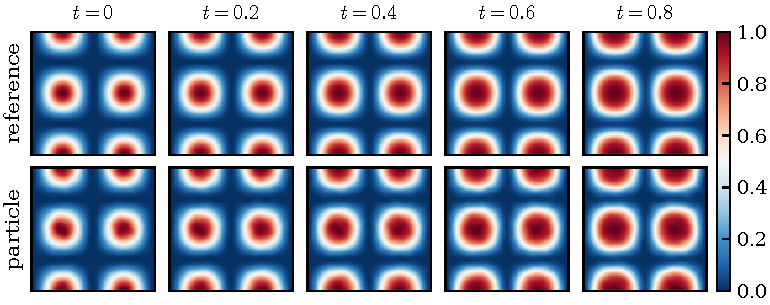
\includegraphics[width=0.8\linewidth]{figure/case_allen_cahn.pdf}
    \caption{Numerical solution of the AC equation \eqref{eq:ac_pde} at different time snapshots ($T=0, 0.2, 0.4, 0.6, 0.8$). The top row displays the reference solution computed by a finite difference method, while the bottom row shows the results from our proposed particle method.}
    \label{fig:ac_solution}
\end{figure}

\textbf{Case 2:} Next, we consider the following KS equation in a periodic domain $\Omega = [0, 2\pi] \times [0, 2\pi]$:
\begin{equation} \label{equ:case1}
\begin{aligned}
&u_t - \nabla \cdot \left(\nabla u - u \nabla v \right) = 0  , &\quad \bx \in \Omega , t > 0, \\
&v_t - \Delta v = u - v , & \quad \bx \in \Omega, t > 0.
\end{aligned}
\end{equation}
The system is subject to periodic boundary conditions, with initial conditions given by:
$$
u_0 (\bx) =  \sin^2(\bx_1) \cos^2(\bx_2), \quad v_0(\bx) =  \cos(\bx_1) + \cos(\bx_2) + 2.
$$
The temporal evolution of the total mass of $v$ is characterized by
$$
M(t) = \int v(t,\bx) \, \intd \bx.
$$
It can be shown that the rate of change of the mass is given by
$$
\dot{M}(t) = -M(t) + \int u(x,0) \, dx = -M(t) + \pi^2.
$$
We present the numerical results for $M(t)$, comparing our method with the exact solution in Figure~\ref{fig:total_mass}.

\begin{figure}[h]
\centering
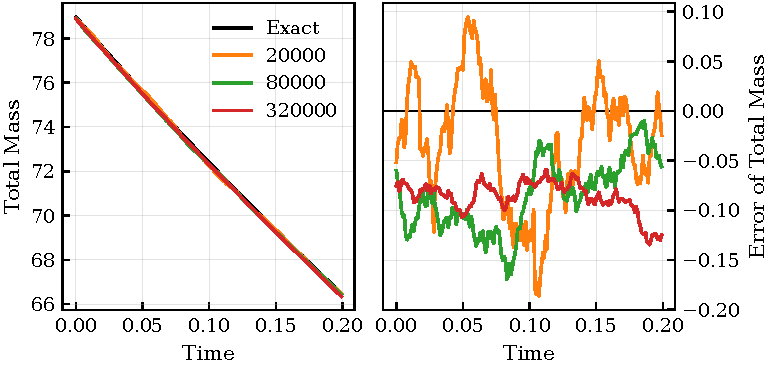
\includegraphics[width=0.8\linewidth]{figure/total_mass.pdf}
\caption{Time evolution of the total mass of $v$ for different numbers of particles. The left panel shows the total mass over time, while the right panel displays the corresponding error in the total mass.}
\label{fig:total_mass}
\end{figure}

Additionally, we compare our particle-based method with finite difference method with a grid of $100 \times 100$ points. The result for $u(t)$ and $v(t)$ at $t = 0.0, 0.1, 0.2, 0.3, 0.4$ are shown in Figures~\ref{fig:fd_comparison_u} and~\ref{fig:fd_comparison_v}, respectively. Figure~\ref{fig:convergence_error} illustrates the reduction in relative $L^2$ error as the number of samples increases, showing a clear $1/\sqrt{N}$ convergence rate.

\begin{figure}[h]
\centering
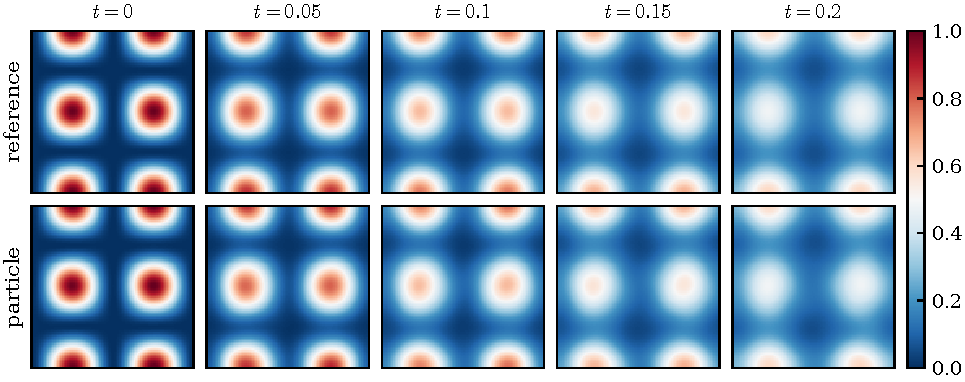
\includegraphics[width=\linewidth]{figure/case1_u.pdf}
\caption{Comparison of the numerical approximation of $u$ obtained from the finite difference method with a $100 \times 100$ grid and the present particle-based method at $t = 0.0, 0.1, 0.2, 0.3, 0.4$.}
\label{fig:fd_comparison_u}
\end{figure}

\begin{figure}[h]
\centering
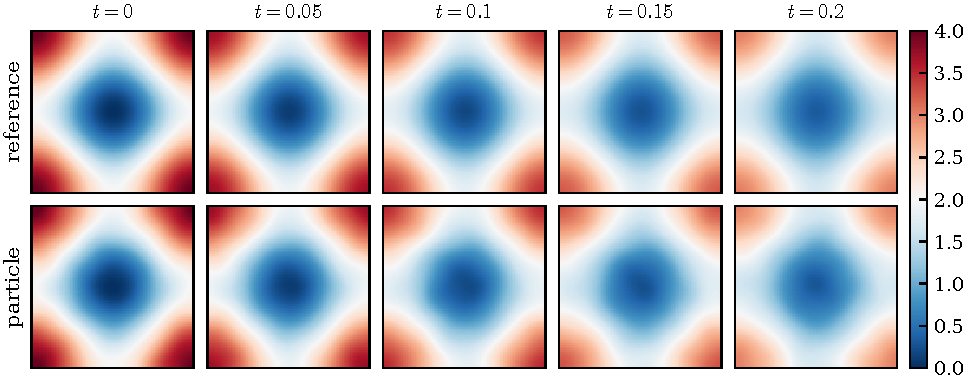
\includegraphics[width=\linewidth]{figure/case1_v.pdf}
\caption{Comparison of the numerical approximation of $v$ obtained from the finite difference method with a $100 \times 100$ grid and the present particle-based method at $t = 0.0, 0.1, 0.2, 0.3, 0.4$.}
\label{fig:fd_comparison_v}
\end{figure}

\begin{figure}[h]
\centering
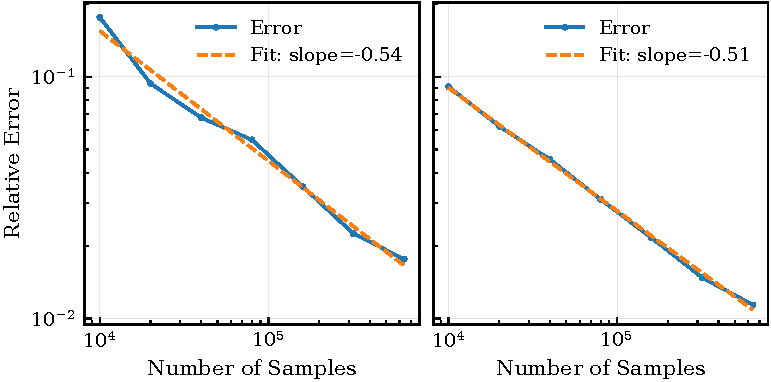
\includegraphics[width=0.8\linewidth]{figure/case1_err.pdf}
\caption{Relative $L^2$ error of $u$ and $v$ with respect to the number of samples $N_0$. The reference solution is obtained with $N_0 = 320,000$.}
\label{fig:convergence_error}
\end{figure}

\textbf{Case 3:} Furthermore, we solve the system \eqref{equ:case1} with the initial conditions:
$$
u_0(\bx) = 840 \exp\left(-84 (\bx_1^2 + \bx_2^2)\right), \quad v_0(\bx) = 420 \exp\left(-42(\bx_1^2 + \bx_2^2)\right).
$$
%
Figure~\ref{fig:case2_u} shows the numerical solution $u$, which undergoes a blow-up phenomenon that is generally difficult to capture using the standard grid discretization. To assess the performance of our method, we compare its results against a finite difference simulation. Three resolution levels are analyzed: the particle method with $N = 40,000$, $160,000$, and $640,000$ is compared to the finite difference method with $200 \times 200$, $400 \times 400$, and $800 \times 800$ mesh points. 
%Our method remains stable with a timestep of $1 \times 10^{-7}$, whereas the finite difference method requires a smaller timestep of $1 \times 10^{-8}$ to avoid earlier blow up of the solution. 
Figure \ref{fig:comparison} shows the numerical solution at $t=5 \times 10^{-5}$. The present particle method enables us to accurately capture the aggregation dynamics and is robust with respect to the number of particles. In contrast, the solution obtained from the finite difference method exhibits pronounced mesh size sensitivity near the aggregation. While the performance of the grid-based approach can be improved by applying more sophisticated spatial discretization such as local discontinuous Galerkin method~\cite{li2017local}, mesh refinement is often required to track the aggregation. On the other hand, the present particle method is natural for modeling such strong nonlinear behaviors without using the adaptive mesh refinement.

% At a fixed reconstruction bandwidth,  the $L^2$ norm of the numerical solution $\tilde{u}$ for different particle counts $N_0$ exhibits similar growth pattern, which indicates robustness with respect to $N_0$, i.e., increasing the particle number primarily reduces the sampling variance but does not change the effective peak shape by the reconstruction. In contrast, the solution obtained from the local discontinuous Galerkin (LDG) method ~\cite{li2017local} exhibits pronounced mesh sensitivity near aggregation, with the observed $L^2$ growth depending strongly on the grid size.

\begin{figure}
\centering
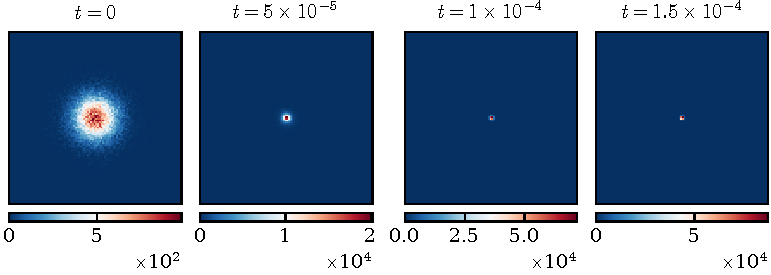
\includegraphics[width=0.8\linewidth]{figure/case2_u.pdf}
\caption{Numerical approximations of $u$ at $t = 0, 5 \times 10^{-5}, 10^{-4}$, and $1.5 \times 10^{-4}$.}
\label{fig:case2_u}
\end{figure}
\begin{figure}
\centering
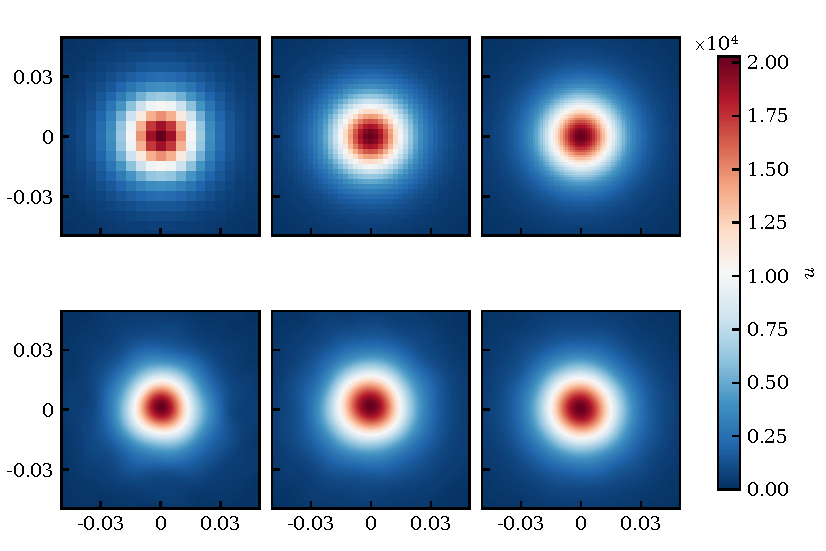
\includegraphics[width=0.85\linewidth]{figure/comparison.pdf}
\caption{Comparison of the numerical solution $u$ from the finite difference method and the present particle method at $t=5\times 10^{-5}$.}
\label{fig:comparison}
\end{figure}
% \begin{figure}
% \centering
% 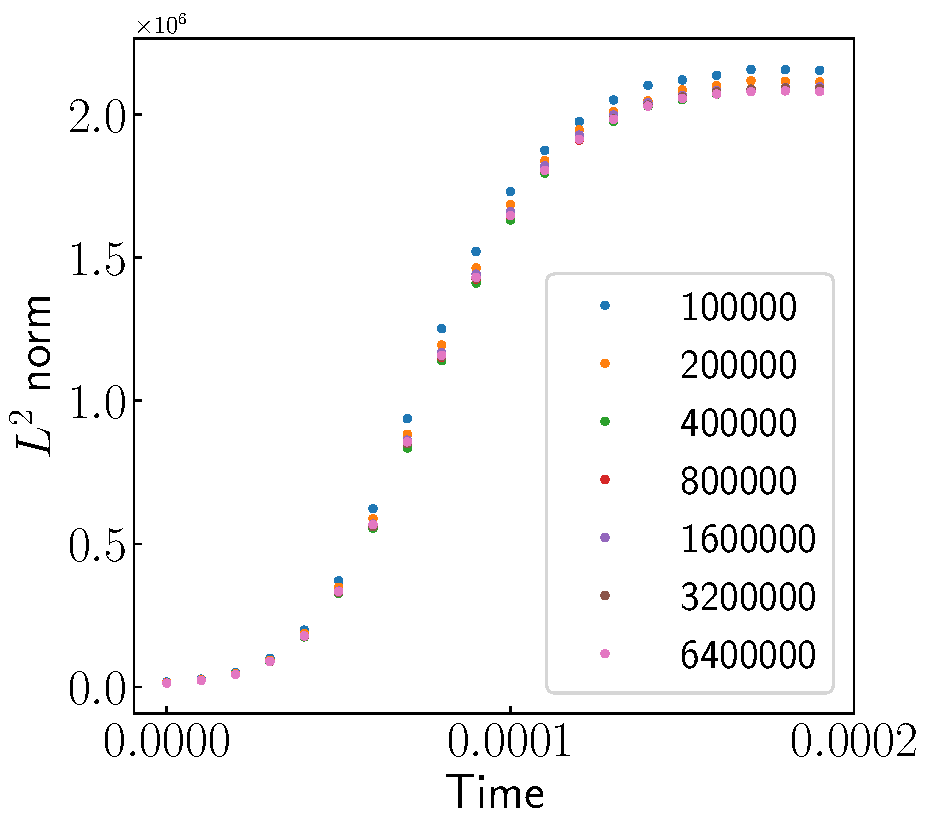
\includegraphics[width=0.5\linewidth]{figure/case2_L2.pdf}
% \caption{Time evolution of the $L^2$-norm of the numerical solution $\tilde{u}$ using different values of $N_0$.}
% \label{fig:case2_l2}
% \end{figure}

\textbf{Case 4:} Finally, we examine a fully nonlinear case with logistic growth for the cells, where the interaction between the particles is not known a priori. The system is given by:
\begin{equation}
\label{equ:nonliear}
\begin{aligned}
&u_t - \nabla \cdot \left(\nabla u - \frac{4u}{1 + u^2} \nabla v \right) = u(1 - u), & \quad \bx \in \Omega, t > 0, \\
&v_t - \Delta v = u - v, & \quad \bx \in \Omega, t > 0.
\end{aligned}
\end{equation}
The theoretical results of this model can be found in \cite{osaki2002exponential, wang2007classical, wrzosek2004global}. The initial conditions are specified as:
$$
    \begin{aligned}
        u_0(\bx) =&  \exp\!\left( -\big[(\bx_1 - 0.5\pi)^2 + (\bx_2 - 0.5\pi)^2\big] \right) + \exp\!\left( -\big[(\bx_1 - \pi)^2 + (\bx_2 - \pi)^2\big] \right) \\
        &+ \exp\!\left( -\big[(\bx_1 - 1.5\pi)^2 + (\bx_2 - 1.5\pi)^2\big] \right), \\
        v_0(\bx) =&  \exp\!\left( -\big[(\bx_1 - 0.4\pi)^2 + (\bx_2 - 0.4\pi)^2\big] \right) + \exp\!\left( -\big[(\bx_1 - 0.8\pi)^2 + (\bx_2 - 0.8\pi)^2\big] \right) \\
        &+ \exp\!\left( -\big[(\bx_1 - 1.2\pi)^2 + (\bx_2 - 1.2\pi)^2\big] \right) + \exp\!\left( -\big[(\bx_1 - 1.6\pi)^2 + (\bx_2 - 1.6\pi)^2\big] \right).
    \end{aligned}
$$

With the non-conservative form, both the birth and death of cells, as well as the chemical concentrations $f_u$ and $f_v$, are non-zero. The particle method proposed in \cite{wang2025novel} only accounts for advection and diffusion and therefore has limited capability in addressing these effects.  In contrast, the present method can naturally handle these additional complexities in the non-conservative form. 
Figures~\ref{fig:case3_u} and~\ref{fig:case3_v} show the time evolution of the solutions $u$ and $v$ obtained using both the particle-based and the finite difference methods.

\begin{figure}
\centering
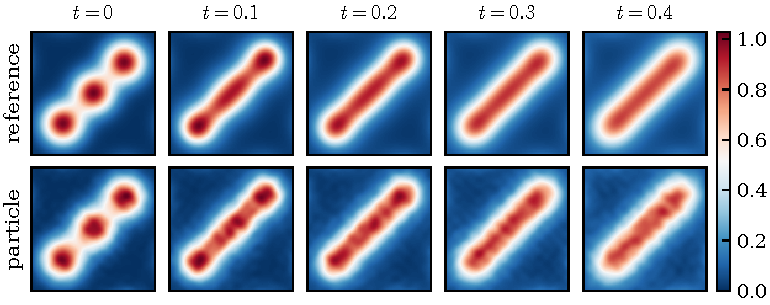
\includegraphics[width=0.8\linewidth]{figure/case3_u.pdf}
\caption{Time evolution of the numerical solution $u$ computed using the particle-based and the finite difference methods.}
\label{fig:case3_u}
\end{figure}

\begin{figure}
\centering
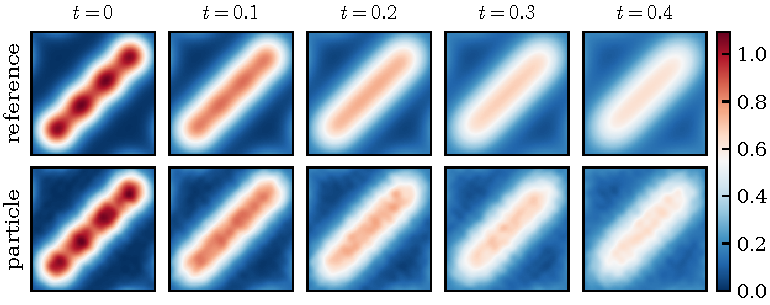
\includegraphics[width=0.8\linewidth]{figure/case3_v.pdf}
\caption{Time evolution of the numerical solution $v$ computed using the particle-based and the finite difference methods.}
\label{fig:case3_v}
\end{figure}

\section{Discussion}
This work presents a stochastic particle-based approach for solving nonlinear non-conservative advection–diffusion–reaction equations. 
The evolution is split into two steps: an advection–diffusion step implemented by particle dynamics, and a local reaction step represented by a stochastic branching birth–death mechanism that provides a consistent temporal discretization of the underlying reaction dynamics. 
Unlike traditional particle or Lagrangian schemes, this formulation enables the present method to naturally capture the non-conservative evolution without an explicit form of the microscopic physical law. The resulting scheme preserves nonnegativity, captures concentration and blow-up robustly, and achieves an unbiased expectation with $O(1/N)$ Monte Carlo variance. Importantly, the algorithm is inherently parallel and does not require grid-based discretization.
%
Numerical results of the AC and the KS equations show the generality and robustness. In particular, the present method accurately captures the nonlinear behaviors such as aggregation and mass evolution of the KS equation without requiring adaptive mesh refinement, and is applicable to a broad class of transport and interaction problems. 

Looking forward, the current work lays the foundation for several promising extensions. From a numerical perspective, the present particle-based formulation is particularly well-suited for high-dimensional PDE problems, where grid-based methods often show limitions. This calls for efficient interpolation of empirical particle measures. In particular, the low-rank spectral approximations and adaptive reconstruction techniques offer promising directions ~\cite{tang2025solving, Peng_Yang_tensor_arxiv_2024}. Additionally, the present method can be extended for more general boundary conditions such as Dirichlet, Neumann, and Robin types, where proper stochastic killing, reflection, or mixed rules need to be developed at the particle level. Finally, while we provide convergence results for the scalar case, theoretical analysis of fully coupled multi-species systems requires further investigation. We leave these for future studies. 

% The framework presented here offers a fresh particle-based approach to solving reaction--diffusion--advection equations. Unlike traditional particle or Lagrangian schemes, our method is not restricted to conservation laws and is able to capture aggregation and focusing phenomena in the density variable with high fidelity. This highlights its potential as a useful tool for studying a broad class of nonlinear transport and interaction problems.

% From the theoretical perspective, the current work provides heuristic intuition primarily in the linear case. Developing a rigorous convergence theory in more general nonlinear settings remains a challenging but exciting direction for future research. On the numerical side, while the interpolation of measures poses difficulties in high-dimensional problems, this limitation also points to promising avenues for methodological innovation. In particular, Fourier interpolation combined with low-rank approximations~\cite{tang2025solving} could provide a powerful mechanism for scaling the algorithm efficiently to higher dimensions.


\section*{Acknowledgments}
The work is supported in part by the National Science Foundation under Grant DMS-2143739 and the ACCESS program through allocation MTH210005. 
The authors also acknowledge the support from the Institute for Cyber-Enabled Research at Michigan State University.


\bibliographystyle{cas-model2-names}
\bibliography{main.bib}

%% else use the following coding to input the bibitems directly in the
%% TeX file.

%% Refer following link for more details about bibliography and citations.
%% https://en.wikibooks.org/wiki/LaTeX/Bibliography_Management

% \begin{thebibliography}{00}

%% For numbered reference style
%% \bibitem{label}
%% Text of bibliographic item

% \bibitem{lamport94}
%   Leslie Lamport,
%   \textit{\LaTeX: a document preparation system},
%   Addison Wesley, Massachusetts,
%   2nd edition,
%   1994.

% \end{thebibliography}
\end{document}

\endinput
%%
%% End of file `elsarticle-template-num.tex'.